% !TeX program = xelatex
%%%%%%%%%%%%%%%%%%%%%%%%%%%%%%%%%%%%%%%%%%%%%%%%%%%%%%%%%%%%%%%%
%%
%% MCI Thesis Template
%% Copyright 2018. David Gollasch.
%%
%%%%%%%%%%%%%%%%%%%%%%%%%%%%%%%%%%%%%%%%%%%%%%%%%%%%%%%%%%%%%%%%

\documentclass[
	11pt, 
	a4paper, 
	twoside, 
	openright, 
	titlepage=firstiscover, 
	numbers=noenddot, 
	BCOR=12mm,
	headsepline,
	footsepline, 
	toc=listof,
	toc=bibliography
	]{scrbook}

%%%%%%%%%%%%%%%%%%%%%%%%%%%%%%%%%%%%%%%%%%%%%%%%%%%%%%%%%%%%%%%%
%%
%% 1. Configure Document
%%
%%%%%%%%%%%%%%%%%%%%%%%%%%%%%%%%%%%%%%%%%%%%%%%%%%%%%%%%%%%%%%%%

\usepackage{import}

%todo: Configure Document

\def\doclanguage{german} %english, german, ngerman	
\def\doctitle{Vergleich datenbasierter Signalgenerierung mittels Machine Learning und Time Series Decomposition}
\def\doctype{Masterarbeit}
\def\docdate{\today}
\def\authorname{Felix Fischer}
\def\authorbirthday{15-07-1998}
\def\authorbirthplace{Wernigerode}
\def\professor{Prof. Dr. rer. nat. habil. Gerhard Weber}
\def\supervisors{M.Sc. Emma Franziska Etzold}

%%%%%%%%%%%%%%%%%%%%%%%%%%%%%%%%%%%%%%%%%%%%%%%%%%%%%%%%%%%%%%%%
%%
%% 2. Take a Look at the Following Predefined Commands
%%
%%	- encoding is utf8 and does not require entities for ä/ö/ü/ß
%%	- generate the document using XeLaTeX instead of pdfLaTeX 
%%	- and Biber engine instead of BibTeX
%%	- Ensure, your TeX distribution is up to date!
%%
%%	- BIB-File is located at includes/bibliography.bib
%%	- abbreviations supported (includes/acronyms.tex)
%%	- multiple columns supported (multicol)
%%	- URLs supported (url)
%%
%%	- definitions and formulae supported
%%		USAGE:
%%		\begin{definition}[<term>]	| \begin{formula}[<term>]
%%		\label{def:<term>}			| \label{for:<term>}
%%			<definition text>		| 	 <formula text>
%%		\end{definition}				| \end{formula}
%%
%%	- listings supported (listings)
%%		USAGE:
%%		inline:
%%			\begin{lstlisting}[caption=<caption>, label=lst:<label>]
%%				<YOUR CODE HERE>
%%			\end{lstlisting}
%%		include:
%%			\lstinputlisting[language=Python]{source_filename.py}
%%
%%	- predefined commands for TODOs
%%		USAGE:
%%		\todo{This is a sandbox todo.}
%%		\todo[Wow]{This as well with own labeling.}
%%		\enhancement{This is an enhancement.}
%%
%%%%%%%%%%%%%%%%%%%%%%%%%%%%%%%%%%%%%%%%%%%%%%%%%%%%%%%%%%%%%%%%

%todo: Look into the available commands

% language constants
\def\english{english}
\def\german{german}
\def\ngerman{ngerman}
\def\true{true}
\def\false{false}

% DOCUMENT LAYOUT SETUP (Encoding, Language, Fonts, Page Setup) 
% 
\usepackage[utf8]{inputenc}	% Encoding

\usepackage{fontspec} % New font management (requires XeLaTeX)
\usepackage{lmodern} % Use (improved) font Latin Modern
\usepackage{amsmath}
% Custom Fonts
\linespread{1.05} % Adjust line spacing, depending on what font you use
\setmainfont{Lora}[
	Path 			= includes/fonts/Lora/ ,
	Extension		= .ttf ,
	UprightFont		= *-Regular ,
	BoldFont		= *-Bold ,
	ItalicFont		= *-Italic ,
	BoldItalicFont	= *-BoldItalic ,
	Scale			= .93 % Adjust font size
	 ]
\setsansfont{Lato}[
	Path 			= includes/fonts/Lato/ ,
	Extension		= .ttf ,
	UprightFont		= *-Regular ,
	BoldFont		= *-Bold ,
	ItalicFont		= *-Italic ,
	BoldItalicFont	= *-BoldItalic ]
\setmonofont{FiraCode}[
	Path 			= includes/fonts/FiraCode/ ,
	Extension		= .otf ,
	UprightFont		= *-Regular ,
	BoldFont		= *-Bold ,
	Scale			= MatchLowercase ]	

\ifx\doclanguage\english
		\usepackage[english]{babel}
\fi
\ifx\doclanguage\german
		\usepackage[german]{babel}
\fi
\ifx\doclanguage\ngerman
		\usepackage[ngerman]{babel}
\fi

\usepackage[left=30mm,right=20mm,top=30mm,bottom=40mm]{geometry} % Page setup

\usepackage[
	pdftoolbar=true,
	bookmarksopen,
	bookmarksnumbered=false,
	bookmarksopenlevel=1,
	pdfdisplaydoctitle,	
    colorlinks,
    citecolor=black,
    filecolor=black,
    linkcolor=black,
    urlcolor=black
]{hyperref} % Linking within PDF
\usepackage[usenames, dvipsnames, svgnames, table]{xcolor} % Manage colours

\xdefinecolor{tudblue}{HTML}{0B2A51}
\xdefinecolor{tudblue2}{HTML}{0059A3}
\xdefinecolor{tudpurple}{HTML}{51297F}
\xdefinecolor{tudpurple2}{HTML}{811A78}
\xdefinecolor{tudgreen}{HTML}{007A47}
\xdefinecolor{tudgreen2}{HTML}{22AD36}
\xdefinecolor{tudorange}{HTML}{E87B14}
\xdefinecolor{codebackground}{rgb}{0.96, 0.96, 0.96}

% FORMAT CONTENT
\usepackage{graphicx} % Graphics options like scale

\usepackage[margin=10pt,font=small,labelfont=bf,labelsep=endash]{caption} % Nicer caption layouts

\usepackage{enumitem} % Customise enumeration formats
	% USAGE:
	%	\begin{enumerate}[label=\lbrack\arabic*\rbrack,start=1]
	%		\item Bla --> (creates [1] Bla)
	%	\end{enumerate}
	%
	%	\begin{enumerate}[label=\lbrack\arabic*\rbrack,resume]
	%		\item Bla --> (creates [2] Bla)
	%	\end{enumerate}
	
\usepackage{multicol} % Introduce multi column content
	% USAGE:
	% \begin{multicols}{<number>}
	% 	<multicolumn text>
	% \end{multicols}

\usepackage{url} % Insert clickable URLs
	% USAGE:
	% \url{http://www.google.com}

% PROVIDE CONTENT

\usepackage[printonlyused,withpage]{acronym} % Manage abbreviations
	% USAGE:
	% Create abbreviations in acronyms.tex this way...
	% 	\acro{POSF}{Partly Open Software Family}
	% 	\acroplural{POSF}[POSFs]{Partly Open Software Families}
	% Call abbreviations anywhere in the document this way...
	% 	\ac{abbr.}         % default:	full at first call, short (abbr.) else
	% 	\acs{abbr.}        % short: 	abbr.
	% 	\acf{abbr.}        % full: 	abbreviation (abbr.)
	% 	\acl{abbr.}        % long: 	abbreviation
	% for plural forms, add a -p: \acp, \acsp, \acfp, \aclp
	
\usepackage{blindtext} % Allow blind text
	% USAGE:
	% \blindtext[4] typesets blind text with 4 repetitions
	% \Blindtext[2][3] typesets blind text with 2 paragraphs and 3 rep.

%======================================================================== BIBLIOGRAPHY

\usepackage[
	backend=biber,
	style=alphabetic,
	maxbibnames=50,
	isbn=false,
	sortlocale=en_UK,
	backref=true,
	backrefstyle=two+
]{biblatex} % User Biber and BibLaTeX

\bibliography{includes/bibliography}
\usepackage{amsmath}
\usepackage{amssymb}
%======================================================================== THEOREMS

\usepackage{mdframed} % Allows framed and coloured environments
\usepackage{thmtools} % Allows Theorem definitions and lists
\usepackage{algorithm}
\usepackage{algpseudocode}
\mdfdefinestyle{guidelinestyle}{
%  linecolor=black,					% STYLE 1 (boxed with grey title)
%  linewidth=.8pt,
%  frametitlerule=true,
%  frametitlefont=\sffamily\bfseries,
%  frametitlebackgroundcolor=codebackground,
%  innertopmargin=\topskip,
  frametitlealignment=\center,		% STYLE 2 (lines top, separator, bottom)
  frametitlefont=\normalfont,
  frametitlerule=true,
  rightline=false,
  leftline=false,
  linewidth=.8pt,
  frametitlerulewidth=.4pt
}
\usepackage{longtable}
\usepackage{pdfpages}
\usepackage{listings}
\usepackage{array}
\usepackage{forest}
\usepackage{booktabs}
\usepackage{adjustbox}
\usepackage{listingsutf8}
\usepackage[utf8]{inputenc}
\makeatletter
\def\namedlabel#1#2{\begingroup
    #2%
    \def\@currentlabel{#2}%
    \phantomsection\label{#1}\endgroup
}
\makeatother

\makeatletter
\define@key{thmdef}{mdthm}[{}]{%
\thmt@trytwice{\def\thmt@theoremdefiner{\mdtheorem[#1]}}{}}
\makeatother

\declaretheorem[
	mdthm={style=guidelinestyle},
	%numberwithin=chapter
]{definition}% <environment name>
\makeatletter
\def\ll@definition{% <environment name>
  \protect\numberline{\csname the\thmt@envname\endcsname}
  \ifx\@empty\thmt@shortoptarg
    \thmt@thmname
  \else
    \thmt@shortoptarg
  \fi}
\makeatother
	% USAGE:
	%\begin{definition}[<term>]
	%\label{def:<term>}
	%	<definition text>
	%\end{definition}
	
\declaretheorem[
	mdthm={style=guidelinestyle},
	%numberwithin=chapter
]{formula}% <environment name>
\makeatletter
\def\ll@formula{% <environment name>
  \protect\numberline{\csname the\thmt@envname\endcsname}
  \ifx\@empty\thmt@shortoptarg
    \thmt@thmname
  \else
    \thmt@shortoptarg
  \fi}
\makeatother
	% USAGE:
	%\begin{formula}[<term>]
	%\label{for:<term>}
	%	<formula text>
	%\end{formula}


%======================================================================== LISTINGS

\usepackage{listings} % add source code inclusion opportunity

\lstset{
	basicstyle=\footnotesize\ttfamily,
	commentstyle=\color{tudgreen2}\ttfamily,
	keywordstyle=\bfseries\color{tudblue2},
	literate={\$}{\$}1,
	captionpos=b,
	language=Java,
	morekeywords={Set, Group, Feature, FeatureModel, Constraint}, 
	numbers=left,  
	numberstyle=\bfseries\ttfamily,
	stepnumber=1, 
	numbersep=5pt,
	tabsize=2,
	texcl=false,
	mathescape=true,
	frame=single,
	framexleftmargin=12pt,
	framextopmargin=1pt,
	framexbottommargin=1pt,
	framexrightmargin=4pt,
	backgroundcolor=\color{codebackground},
	showspaces=false,
	showstringspaces=false,
	numberbychapter=true
}

\lstdefinelanguage{JavaScript}{
  keywords={typeof, new, true, false, catch, function, return, null, catch, switch, var, if, in, while, do, else, case, break},
  keywordstyle=\color{blue}\bfseries,
  ndkeywords={class, export, boolean, throw, implements, import, this},
  ndkeywordstyle=\color{darkgray}\bfseries,
  identifierstyle=\color{black},
  sensitive=false,
  comment=[l]{//},
  morecomment=[s]{/*}{*/},
  commentstyle=\color{purple}\ttfamily,
  stringstyle=\color{red}\ttfamily,
  morestring=[b]',
  morestring=[b]'
}
\lstdefinelanguage{PowerShell}{
  morekeywords={param, foreach, in, if, else, function, return, Write-Host},
  morecomment=[l]{\#},
  morestring=[b]',
  morestring=[b]'
}
	% USAGE:
	% inline:
	%	\begin{lstlisting}[caption=<caption>, label=lst:<label>]
	%		<YOUR CODE HERE>
	%	\end{lstlisting}
	% include:
	%	\lstinputlisting[language=Python]{source_filename.py}

%======================================================================== COLOURS

	% USAGE:
	% \textcolor{tudblue}

%======================================================================== TODOs
%-TODO Tag with optional comment
%(#1: comment) #2: affected region
\newcommand{\todo}[2][TODO]{\textbf{\textcolor{tudpurple2}{[#1]} \textcolor{tudorange}{#2}}}
%-ENHANCEMENT Tag
\newcommand{\enhancement}[1]{\textcolor{tudpurple2}{[Enhancement]} \textcolor{tudblue2}{#1}}
	% USAGE:
	% \todo{This is a sandbox todo.}
	% \todo[Wow]{This as well with own labeling.}
	% \enhancement{This is an enhancement.}


\newcommand{\personadetail}[2]{\noindent\makebox[5cm][l]{\textbf{#1}:}\hspace{0.5em}#2\\}



\begin{document}
\pagenumbering{gobble}

\newgeometry{margin=1in, top=2.5in}

\begin{titlepage}
% front page

\begin{center}

	{\large
		\doctype\relax
	}
	
	\vspace{.5cm}
	
	{\huge \bfseries \sffamily
		\doctitle\relax
		\par
	}
	
	\vspace{1.5cm}
	
	\ifx\doclanguage\english
		submitted by
	\fi
	\ifx\doclanguage\german
		eingereicht von
	\fi
	\ifx\doclanguage\ngerman
		eingereicht von
	\fi
	
	\vspace{.5cm}
	
	\textbf{\authorname} \\
	\ifx\doclanguage\english
		born
	\fi
	\ifx\doclanguage\german
		geboren am
	\fi
	\ifx\doclanguage\ngerman
		geboren am
	\fi
	\authorbirthday{} in \authorbirthplace

	
	\vspace{1.5cm}
	
	{\Large Technische Universität Dresden}
	
	\vspace{.5cm}
	
	\ifx\doclanguage\english
		Faculty of Computer Science \\
		Institute of Applied Computer Science \\
		Chair of Human-Computer Interaction

	\fi
	\ifx\doclanguage\german
		Fakultät Informatik \\
		Institut für Angewandte Informatik \\
		Lehrstuhl Mensch-Computer-Interaktion

	\fi
	\ifx\doclanguage\ngerman
		Fakultät Informatik \\
		Institut für Angewandte Informatik \\
		Lehrstuhl Mensch-Computer-Interaktion

	\fi
	
	\vspace{1.0cm}
	
	
\includegraphics[scale=.75]{includes/figures/tu_logo}
	
	\vspace{1.5cm}
\end{center}

	\noindent
	\ifx\doclanguage\english
		Supervisors: \\
	\fi
	\ifx\doclanguage\german
		Betreuer: \\
	\fi
	\ifx\doclanguage\ngerman
		Betreuer: \\
	\fi
	\supervisors
	
	\vspace{.5cm}
	
	\noindent
	\ifx\doclanguage\english
		Professor: \\
	\fi
	\ifx\doclanguage\german
		Hochschullehrer: \\
	\fi
	\ifx\doclanguage\ngerman
		Hochschullehrer: \\
	\fi
	\professor
	
	\vspace{1.5cm}
	
	\noindent
	\ifx\doclanguage\english
		Submitted
	\fi
	\ifx\doclanguage\german
		Eingereicht am
	\fi
	\ifx\doclanguage\ngerman
		Eingereicht am
	\fi
	\docdate


% Add PDF Meta Data
\hypersetup{
		pdftitle={\doctitle},
		pdfauthor={\authorname},
		pdfsubject={\doctype}
	}

\end{titlepage}

\restoregeometry


%todo: Include thesis task description here
% You got it from your supervisor. Scan the document and
% include it as full-page PDF here. If your task description
% is larger than 3 pages, consider putting it in the appendix 
% instead.

% Confirmation
\ifx\doclanguage\english
	\chapter*{Confirmation}
	I confirm that I independently prepared this thesis with the title 
	\emph{\doctitle}
	and that I used only the references and auxiliary means indicated in the thesis.

\fi
\ifx\doclanguage\german
	\chapter*{Erklärung}
	Ich erkläre, dass ich die vorliegende Arbeit mit dem Titel 
	\emph{\doctitle}
	selbständig unter Angabe aller Zitate angefertigt und dabei ausschließlich die aufgeführte Literatur und genannten Hilfsmittel verwendet habe.
\fi
\ifx\doclanguage\ngerman
	\chapter*{Erklärung}
	Ich erkläre, dass ich die vorliegende Arbeit mit dem Titel 
	\emph{\doctitle}
	selbständig unter Angabe aller Zitate angefertigt und dabei ausschließlich die aufgeführte Literatur und genannten Hilfsmittel verwendet habe.
\fi

\vspace{1.5cm}

\noindent
Dresden, \docdate

\vspace{3.0cm}

\noindent
\authorname

 %todo: Sign the confirmation
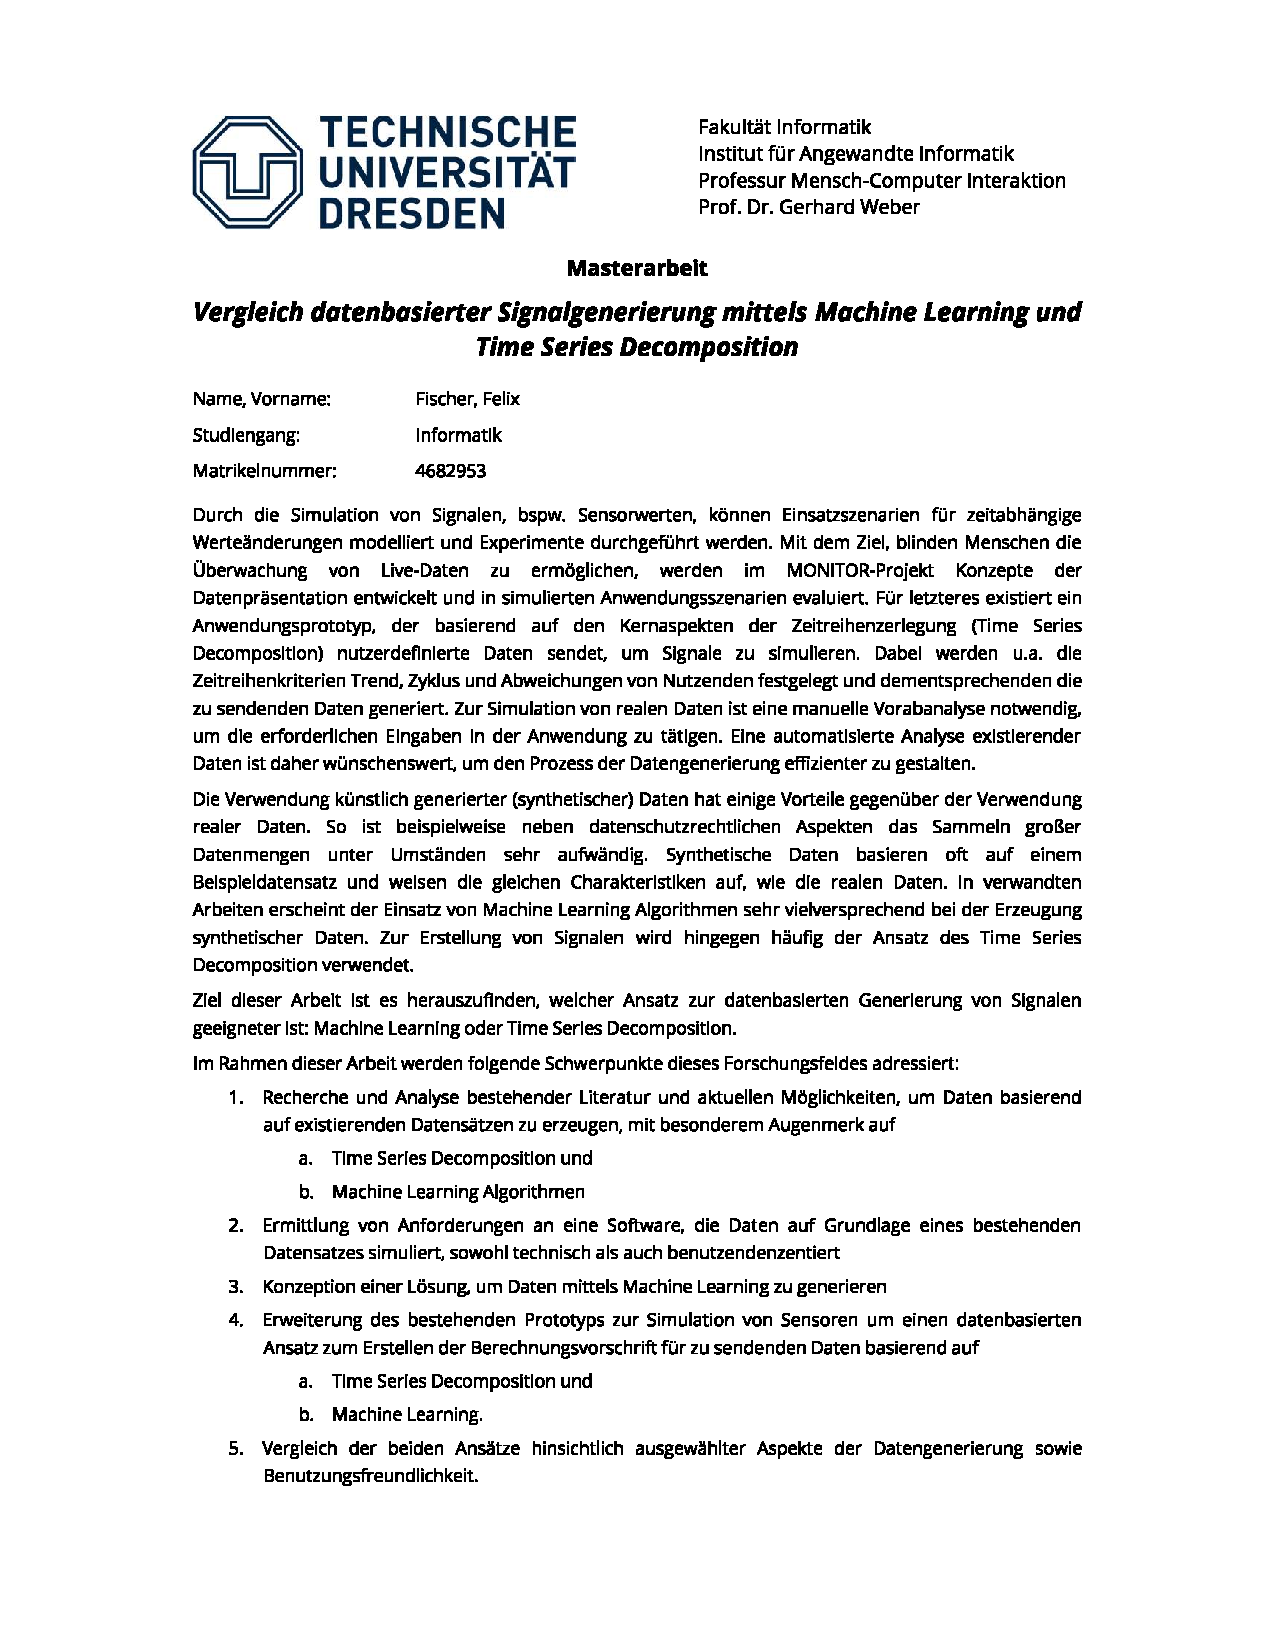
\includepdf[pages=-]{pdfs/Aufgabenstellung_FelixFischer_printed.pdf}
\cleardoublepage
\pagenumbering{Roman}

%todo: Write an abstract
\chapter*{Abstrakt}

Die vorliegende Masterarbeit erforscht die Generierung synthetischer Datenströme unter Einsatz von Machine Learning-Methoden und traditioneller Zeitreihenzerlegung, 
insbesondere im Kontext des MONITOR-Projekts. Angesichts der zunehmenden Bedeutung synthetischer Daten, wie durch frühe Entwicklungen autonomer Fahrzeuge und deren Einsatz 
von KI illustriert, widmet sich diese Arbeit der Fragestellung, wie numerische Datenströme effektiv generiert werden können. Dabei liegt der Fokus auf der Simulation von Sensordaten in verschiedenen Szenarien.

Zentraler Bestandteil dieser Arbeit ist der Vergleich zwischen Machine Learning-Ansätzen und traditionellen mathematischen Modellen zur Zeitreihenzerlegung. 
Beide Methoden werden hinsichtlich ihrer Effizienz, Genauigkeit und Anwendbarkeit in der Simulation von Datenströmen evaluiert. Es wird untersucht, inwieweit generative oder rekursive 
Modelle im Vergleich zu einfacheren, ressourcenschonenden mathematischen Modellen wie ARIMA oder Empirical Mode Decomposition zur Rekonstruktion von Zeitreihen eingesetzt werden können.

Ein wesentliches Ziel der Arbeit ist die Entwicklung und Implementierung eines Konzepts, das beide Ansätze in einer bestehenden Simulationsumgebung integriert. Dieses Konzept soll nicht nur die 
technischen Aspekte abdecken, sondern auch benutzerfreundlich gestaltet sein, um auch Nicht-Experten im Bereich des maschinellen Lernens den Zugang zu ermöglichen.

Abschließend zielt diese Arbeit darauf ab, einen wissenschaftlichen und praktischen Beitrag zu leisten, indem sie komplexe Methoden der Datengenerierung zugänglicher macht und tiefere Einblicke 
in die Dynamik und Potenziale beider Ansätze bietet. Dadurch sollen innovative Anwendungen und Forschungsmöglichkeiten in verschiedenen Bereichen eröffnet werden. Die Ergebnisse dieser Arbeit sollen Nutzern helfen, 
fundierte Entscheidungen bei der Wahl der geeigneten Methode zur Datenstromgenerierung zu treffen.



\tableofcontents

\cleardoublepage
\pagenumbering{arabic}

%todo: Write you thesis content
% !TeX program = xelatex

\chapter{Einleitung}
Die Bedeutung synthetischer Daten wurde bereits in den frühen Entwicklungsphasen autonomer Fahrzeuge in den 1980er Jahren deutlich. 
Ein markantes Beispiel hierfür ist der "Navlab I" \cite{NeuralNe96:online}, ein experimentelles autonomes Fahrzeug der Carnegie Mellon University, welches mit vier leistungsstarken Computern ausgestattet 
über den Campus fuhr und somit eine Schlüsselrolle in der Evolution der künstlichen Intelligenz spielte. Die Herausforderung, verschiedene Fahrszenarien allein mit einem Satz von Instruktionen abzudecken, 
die manuell gesammelt werden mussten, führte zu einem bedeutsamen Paradigmenwechsel hin zum Einsatz von maschinellem Lernen. Dean Pomerleau nutzte, anstatt alle Situationen selbst aufzubauen, ein Set an Daten, 
um weitere Situationen durch synthetische Daten zu generieren. Seine Pionierarbeit in der Entwicklung neuronaler Netze, die mit synthetischen Straßenbildern trainiert wurden, illustriert eindrucksvoll die wachsende Bedeutung von synthetischen Daten.

In der heutigen Ära, die durch einen erneuten AI-Boom und die Verfügbarkeit von leistungsstarken Computerplattformen gekennzeichnet ist, gewinnen synthetische Daten weiter an Bedeutung. Vor diesem Hintergrund widmet 
sich diese Arbeit der Untersuchung des Mehrwerts von maschinellem Lernen bei der Generierung von numerischen Datenströmen und stellt diese Methodik der traditionellen Zeitreihenzerlegung gegenüber.

Diese Arbeit untersucht Machine Learning-Methoden im Vergleich zur traditionellen Zeitreihenzerlegung zur Generierung von numerischen Datenströmen, im Kontext des MONITOR-Projekts, das die Entwicklung und Evaluation 
von Datenpräsentationskonzepten in simulierten Anwendungsszenarien verfolgt. Der Fokus liegt auf der Simulation von Signalen, speziell Sensorwerten, die zeitabhängige Veränderungen in verschiedenen Szenarien modellieren. 
Ziel ist es, die Wirksamkeit und Effizienz von Machine Learning gegenüber der Time Series Decomposition zu bewerten, Methoden zu analysieren, Anforderungen an entsprechende Software zu formulieren und einen Lösungsansatz 
basierend auf Machine Learning zu entwickeln. Zusätzlich wird ein bestehender Prototyp zur Sensordatensimulation erweitert, um beide Ansätze zu implementieren und zu vergleichen.

\section{Motivation}
Die Simulation von Daten stellt eine komplexe Herausforderung dar, die sich durch verschiedene Ansätze charakterisiert und in Genauigkeit, Geschwindigkeit und Komplexität unterscheidet.

Aber zum ersten Thema. Die Frage, welcher Ansatz der richtige ist, hängt von zahlreichen Faktoren ab und ist von entscheidender Bedeutung in einer datengetriebenen Welt.

In den folgenden Kapiteln dieser Arbeit werden verschiedene Methoden zur Generierung synthetischer Daten aus bestehenden Datenquellen diskutiert. Insbesondere rücken generative Modelle, die

bereits in vielen Bereichen der Bild- und Tabellengenerierung eingesetzt werden, in den Vordergrund. Diese Modelle müssen nur einmal trainiert werden und können daraufhin Daten erzeugen, die den Originaldaten sehr nahekommen. 
Jedoch stellt dies auch hohe Anforderungen an die Rechenkapazität und ist in seiner Komplexität nicht zu unterschätzen. Besonders im Bereich der Zeitreihenanalyse scheinen diese Ansätze noch nicht umfassend erforscht zu sein, 
was den Einstieg in diesen speziellen Forschungsbereich spannend macht.

Eine Alternative bieten mathematische Modelle, die zwar weniger flexibel, aber deutlich ressourcenschonender sind. Solche Modelle, die bereits in verschiedenen Sektoren wie im Finanzwesen zur Vorhersage von Marktentwicklungen 
eingesetzt werden, könnten auch zur Rekonstruktion von Zeitreihen genutzt werden. Modelle wie ARIMA oder Facebooks Prophet, die darauf abzielen, Informationen aus Daten zu extrahieren, könnten somit verwendet werden, um eine den 
Originaldaten nahekommende Zeitreihe zu generieren. Der Vergleich dieser einfacheren Ansätze mit den komplexeren generativen Modellen ist daher ein Kernaspekt dieser Arbeit.

In dieser Masterarbeit sollen die beiden Ansätze, Machine Learning und Zeitreihenzerlegung, gegenübergestellt werden. Beide haben ihre spezifischen Vor- und Nachteile, und die Wahl des geeigneten Ansatzes hängt von den jeweiligen 
Anforderungen ab. Das Ziel dieser Arbeit ist es daher, Erkenntnisse zu liefern, die die Entscheidungsfindung für die geeignete Methode erleichtern.

Darüber hinaus soll ein Konzept entwickelt und umgesetzt werden, das diese Ansätze praktikabel macht und sie in eine existierende Simulationsumgebung integriert. Dieses Konzept soll nicht nur die technischen Aspekte abdecken, 
sondern auch benutzerfreundlich gestaltet sein, sodass auch Personen ohne tiefgehende Kenntnisse im Bereich des maschinellen Lernens davon profitieren können. Der Vergleich der Ansätze wird aufzeigen, welcher Weg für bestimmte 
Anforderungen am besten geeignet ist, und Nutzern helfen, eine fundierte Entscheidung zu treffen.

Diese Arbeit soll nicht nur einen wissenschaftlichen Beitrag leisten, sondern auch praktische Anwendungen in verschiedenen Bereichen ermöglichen, indem sie komplexe Methoden zugänglicher macht. Die Motivation dahinter ist es, 
ein tieferes Verständnis für die Dynamik und Potenziale beider Ansätze zu schaffen und so die Tür für innovative Anwendungen und Forschung in der Zukunft zu öffnen.

\section{Zielsetzung}
Es handelt sich um eine zweiteilige Arbeit. Einerseits muss die bestehende Simulationsumgebung in vielen Punkten verändert und erweitert werden, da sie aktuell

nur die Generierung von Daten mittels Zeitreihenzerlegung beinhaltet und fast keine Flexibilität in der Art der gesendeten Daten bietet. Auch muss das Gesamtprojekt durch eine weitere \acf{API} zur Bereitstellung der 
Methoden des maschinellen Lernens und der Zeitreihenanalyse erweitert werden. Diese muss sich in die bestehende Architektur integrieren lassen und die Möglichkeit bieten, die Daten in derselben Form wie die Zeitreihenzerlegung 
zu erhalten. Auch steht eine nutzerfreundliche Oberfläche im Vordergrund, welche es gerade fachfremden Nutzern ermöglicht, diese Software zu verwenden.

Auf der anderen Seite steht eine Evaluation der bestehenden Konzepte und Methoden an. Es muss analysiert werden, wann und warum es sinnvoll ist, sich für eine der beiden Varianten zu entscheiden. Hierzu müssen die Vor- 
und Nachteile der beiden Ansätze gegenübergestellt werden und die Ergebnisse der beiden Ansätze verglichen werden.
% !TeX program = xelatex

\chapter{Ausgangslage und Stand der Technik}
\label{cha:stateOfTheArt}

\section{Ansätze aus dem Bereich des maschinellen Lernens}

\subsection{SynGen: Synthetic Data Generation}

SynGen, ein von Akash Kothare et al.\cite{9697232} entwickeltes Instrument zur Synthese von Daten, wurde auf der ICCICA 2021 (International Conference on Computational Intelligence and Computing Applications) präsentiert.
Das Tool folgt einem dreistufigen Prozess zur Generierung von Benutzerdaten, der Flexibilität und Anpassungsfähigkeit in der Datenproduktion bietet.

In der Initialisierungsphase bietet SynGen Benutzern die Wahl, entweder ein Beispielset zu importieren oder durch die Spezifikation von Feldnamen und der gewünschten Zeilenzahl einen neuen
Datensatz zu generieren, wobei letzteres durch den Einsatz von Faker\cite{Faker} als Grundlage für die Datenerstellung dient.

Daraufhin wird im zweiten Schritt des Prozesses die maschinelle Lernstrategie gewählt. Das Tool stellt verschiedene Implementierungen des überwachten Lernens für Regression und
Klassifikation sowie des unüberwachten Lernens zur Verfügung. Diese Auswahl ermöglicht es dem Benutzer, die Methode zu wählen, die am besten zu den Anforderungen der spezifischen Daten und des intendierten Anwendungsfalls passt.

Im abschließenden Verfahrensschritt ermöglicht der Similarity Index der Modelle eine Evaluation der Leistungsfähigkeit der verschiedenen Algorithmen. Um diese Bewertung zu vereinfachen,
verwendet SynGen ein Effizienzvergleichsdiagramm sowie eine Konfusionsmatrix, die die Genauigkeit der Modelle illustriert und somit eine direkte und nutzerfreundliche Methode zur Bewertung der Modellqualität bietet.


\subsection{GenEthos}
Im Rahmen der fortschreitenden Entwicklung synthetischer Datengenerierungssysteme stellt das Werk von Shubham Gujar et al.\cite{9885653}, "GenEthos",
ein innovatives GUI-basiertes Tool dar. Dieses System zeichnet sich durch seine Fähigkeit aus, nicht nur synthetische Daten zu erstellen,
sondern auch eine kontinuierliche Überwachung und Bias-Detektion für die generierten Modelle zu ermöglichen.
Zur Bewahrung logischer Konsistenzen innerhalb der erzeugten Datenmengen integriert GenEthos die Principal Component Analysis (PCA) und Learning Fair Representations (LFR).
PCA dient hier als eine Technik zur Dimensionsreduzierung, die Daten aus einem hochdimensionalen in einen niedrigeren Raum transformiert, während die maximale
Informationsmenge erhalten bleibt\cite{PCA_Explained}. LFR wird als Vorverarbeitungsmethode verwendet, um diskriminierende Merkmale aus den Daten zu entfernen\cite{LFR_Explained}.

Darüber hinaus präsentieren die Autoren ein benutzerdefiniertes Konzept für die kategorische Erstellung von Benutzeroberflächen, das es dem Nutzer ermöglicht,
die Datenbeziehungen durch vordefinierte Ausdrücke wie Zufallsfunktionen oder Bedingungen anzupassen oder sogar eigene Python-Funktionen zu implementieren, um Verknüpfungen zwischen den Tabellenspalten zu modifizieren oder zu generieren.

Die Datenerstellung erfolgt unter Verwendung von Faker\cite{Faker} für den anfänglichen Input und fünf unterschiedlichen Modellen für die Datenmodellierung:

\begin{description}
    \item[\namedlabel{genethos:tgan}{T-GAN}] bietet eine auf tabellarische Daten spezialisierte GAN-Variante.
    \item[\namedlabel{genethos:gretel}{Gretel}] verwendet LSTM-basierte Netzwerke und legt den Fokus auf Datenschutz.
    \item[\namedlabel{genethos:CTGAN}{CTGAN}] repräsentiert einen weiteren GAN-basierten Ansatz für die Modellierung tabellarischer Daten und die Generierung von Datenzeilen aus einer Verteilung.
\end{description}

Zur Bewertung von Fairness und zur Minderung ethischer Voreingenommenheit wurden zusätzlich Metriken wie Statistical Parity Difference und Disparate Impact sowie Algorithmen wie Prejudice Remover,
Disparate Impact Remover und Learning Fair Representations verwendet. Diese Methoden liegen jedoch außerhalb des Umfangs dieser Arbeit.

In der Evaluation ihres Systems verwendeten die Forscher die Adult- und German Credit Datensätze, um Fairness und Bias zu untersuchen und führten Vergleiche mit synthetischen Daten aus den oben
genannten Modellen durch. Alle drei Modelle replizierten die vorhandenen Daten mit geringfügigen Bias-Abweichungen effektiv. Die Hauptzielsetzung der Studie war es, den Beitrag von
Algorithmen zur Bias-Entfernung zu bewerten. Dabei wurde festgestellt, dass zwar eine Reduktion von Bias möglich ist, diese jedoch ihre Grenzen hat.


\subsection{Synthetic Test Data Generation Using Recurrent Neural Networks: A Position Paper}
In der Untersuchung von Razieh Behjati et al.\cite{8823801} wird der Einsatz von Long Short-Term Memory (LSTM) Netzwerken zur Generierung von synthetischen Testdaten für ereignisgesteuerte Systeme beleuchtet.
Diese Forschung findet im Rahmen des Upgrades des norwegischen nationalen Registers statt, einem Kontext, der eine hohe Sensibilität für den Datenschutz erfordert. Synthetische Daten dienen hier als
Alternative zu realen Produktionsdaten, insbesondere wenn letztere persönliche Informationen enthalten, die nicht für Tests freigegeben werden können.

Das Team hat einen Ansatz verfolgt, bei dem Eingabedaten in sogenannte Meta-Events segmentiert wurden, die jeweils eine Klassifizierung und assoziierte personenbezogene Daten enthielten.
Diese methodische Aufteilung ermöglichte es dem LSTM-Modell, die Struktur und essentiellen Muster der Daten – wie die Zuordnung von Monaten zu deren maximaler Tagesanzahl – effektiv zu lernen.

Während das Modell Basisabhängigkeiten mit Erfolg reproduzieren konnte, zeigte sich bei der Abbildung komplexerer Regeln, wie der Berücksichtigung von Schaltjahren, eine gewisse
Begrenzung. Dies lässt sich potenziell auf die Größe des Trainingsdatensatzes zurückführen und weist auf den Bedarf an umfangreicheren Daten für das Training fortgeschrittener Sequenzmodellierung hin.


\subsection{Generation of Synthetic Continuous Numerical Data Using Generative Adversarial Networks}

In ihrer Studie untersuchen A H Aziira und Kollegen\cite{Aziira_2020} die Anwendung von Generative Adversarial Networks (GANs) zur Erzeugung kontinuierlicher numerischer Daten für unüberwachte maschinelle
Lernprozesse (Unsupervised Machine Learning Tasks). Die Kernforschung evaluiert die Effizienz von GANs und Conditional GANs (CGANs) bei der Generierung authentischer Datensätze durch ein gezieltes Experiment mit begrenztem Umfang.

Für das Experiment bedienten sich die Autoren des öffentlichen Datensatzes
WornBlade002\footnote[1]{Dieser Datensatz stammt von Schneidmessern der Vega
    Schrumpffolienproduktion und dient der Überwachung der Maschinenperformance.}, um die Performance eines GAN und eines CGAN zu trainieren und zu beurteilen.
Die Authentizität der generierten Daten wurde durch zwei komplementäre Methoden geprüft: qualitative Bewertungen zur Beurteilung der Übereinstimmung der
Datenverteilung mit dem Originaldatensatz und quantitative Maßnahmen zur Einschätzung der Realitätsnähe der synthetisierten Daten. Letztere basierten auf
dem XGBoost-Algorithmus – einem Gradient Boosting Framework für baumbasierte Lernmodelle –, der auf einer Kombination von echten und generierten Daten trainiert wurde.
Die Genauigkeit der Modelle wurde mittels einer Konfusionsmatrix evaluiert, mit dem Ziel, eine Genauigkeit (Accuracy) von 50\%
zu erreichen, was eine Ununterscheidbarkeit zwischen echten und generierten Daten suggerieren würde.

\begin{equation}
    accuracy = \frac{TP + TN}{TP + TN + FP + FN} *  100\%
\end{equation}

Zusätzlich wurde der Mann-Whitney-U-Test angewandt, um die statistische Signifikanz der Unterschiede zwischen den echten und generierten
Datenstichproben zu ermitteln und Tendenzen der Abhängigkeit aufzudecken\cite{MannWhit25:online}.

Die Ergebnisse des Experiments zeigen, dass nach ungefähr 10.000 Trainingsschritten die Genauigkeitswerte der GANs und CGANs nur noch marginal
verbessert werden konnten. Mit einer maximalen Genauigkeit von 55\% für die CGANs demonstrieren die Ergebnisse eindrucksvoll, dass
GANs prinzipiell fähig sind, kontinuierliche numerische Daten mit hoher Qualität zu generieren.

\section{Zeitreihenanalyse- und Zerlegung}

\subsection{The empirical mode decomposition and the Hilbert spectrum for nonlinear and non-stationary time series analysis}
Huang u.w.\cite{doi:10.1098/rspa.1998.0193,} arbeiteten an einer neuen Methode um komplexe,
nicht-lineare\footnote{Bei nicht-linearen Daten zeigt die Beziehung zwischen abhängigen und unabhängigen Variablen keine gerade Linie.} und
nicht-stationäre\footnote{Im Kontext von Time Series sind nicht-stationäre Daten Segmente oder Teile, die unabhängig von der Zeit Ihre Werte besitzten.} Daten zu analysieren.


Dafür nutzten sie eine \acp{EMD}, eine Methode zum Zerlegen von komplexen Daten endliche, meist kleine Anzahl von \acp{IMF}, welche zwei Regeln befolgen müssen.
\begin{enumerate}
    \item Die Anzahl an Maxima und Nullpunkten sollte möglichst 0 sein.
    \item An jedem Punkt sollte die Summe des lokalen Maximums und Minimums 0 sein.
\end{enumerate}

Hierdurch werden Maxima und Minima mit Splines verbunden und daraufhin die Mittelwerte der Maxima- und Minimaanstiege aus dem Signal entfernt.
Dieser Prozess ist iterativ und wiederhohlt sich, bis keine Maxima mehr vorhanden sind.
Da dies teilweise zu Problemen führt, wurde der Algorithmus 2003 von Huang Daji u.w.\cite{daji2003practical} angepasst,
indem eine \acp{EEM} eingeführt wurde, welche das Signal um erste und letzten lokale Extrema erweitert. Diese werden bei der späteren Berechnung besonders behandelt.

Aus den einzelnen \ac{IMF}s, welche man mit oszilierenden Funktionen vergleichen kann, werden genutzt um durch eine \acp{HSA} über einen Zeitparameter das Signal zu rekonstruieren.
Die Summe der einzelnen Funktionen kann somit das originale Signal rekonstruieren.
\begin{equation}
    X(t) = \sum_{i=1}^{M} IMF_{i} + r(t)
\end{equation}

Während das \acp{HHT}, wie die Methode auch genannt wird, viele verschiedene Einsatzgebiete, von
Biomedizin über Ozeanographie bis Seismographie, hat, ist gerade die Glättungsfunktion der \ac{EMD} in vielen Bereichen besonders relevant.
% kann genommen werden um random aspekte aus signal zu entfernen


\subsection{Singular Spectrum Decomposition: a New Method for Time Series Decomposition}
In \cite{doi:10.1142/S1793536914500113} stellten PIETRO BONIZZI Pietro Bonizzi u.w. eine neue Methode zur Aufspaltung von nichtlinearen, nichtstationären Zeitreihen vor.

Aufbauend auf \ac{SSA} (siehe \ref*{techniques:SSA}), lieferten sie einen innovativen Ansatz, welcher das bestehende \ac{SSA} Prinzip übernimmt, den dahinterliegenden Algorithmus aber überarbeitet.
So wird beispielsweise die Trajektorienmatrix angepasst und fokussiert sich stärker auf die oszilierenden Komponenten des Signales.
Im Zerlegungsprozess ist ein Fokus auf die Frequenzen somit einfacher und dies erlaubt wiederum aussagekräftige Komponenten zu isolieren.
Eine weitere wichtige Neuerung ist die Auswahl von Hauptkomponenten zu automatisieren. Dieser in SSA noch manuelle Schritt


Es erlaubt somit einen Fokus auf die Frequenzen und kann somit besser die Frequenzen isolieren aber die Auswahl der Parameter wie window-length automatisiert und somit nicht für die jeweiligen Daten neu angepasst werden muss.


\subsection{Synthetic Data by Principal Component Analysis}
In dem Paper \cite{9346379} zur synthetischen Datengenerierung stellt Natsuki Sano zwei Methoden vor. Beide zielen darauf ab aus realen Daten (Daten aus von Decathlon organisierten Sport Events wie Weitsprung, Hochsprung und Sprint), die persönlichen Aspkete zu entfernen,
aber die Eigenschaften der Daten an sich beizubehalten. Dies steht entegegen dem Konzept des Maskierens von Daten um Annonymität zu erreichen.
Für die generierung wird ein linearer und ein nicht linearer Ansatz vorgesetllt.

\paragraph*{Orthogonale Transformation}
ist eine Methode welche auf \acf{PCA} setzt. \ac{PCA} ist eine statistisches Analyseverfahren, welches große Datenmengen in kleinere, den inhalt zusammenfassende Sets aufteilt. Diese sind dadurch leichter zu analysieren.
Aber \ac{PCA} ist lediglich in der Lage den linearen Zusammenhang zwischen Variablen zu analysieren und darzustellen.
Interessant ist dieser Ansatz, da er eine direkte Bewertung des Verfahrens zulässt. Duch die im Prozess verworfenen Eigenwerte kann der Informationsverlust bestimmt werden.

\paragraph*{Sandglass-Type Neural Networks}
Für nicht-lineare Zusammenhänge kann normale \ac{PCA} nicht eingesetzt werden, Da aber nicht alle Zusammenhänge innerhalb der Daten linearer Natur sind, wird ein anderer Ansatz gebraucht, dier kommt in Form von Sandglass Neural Networks.
Diese Sanduhr Förmigen Netzwerke besitzten eine stark eingeschränkte Zwischenschicht, ähnelt daher einer Sanduhr. Dies sorgt dafür, dass die originalen Daten in der Zwischenschicht stark reduziert werden um dann in der Ausgangsschicht aus der komprimierten Version die Daten wieder zu rekonstruieren.
Somit kann Machine Learning im \ac{PCA} Verfahren eingesetzt werden komplexe Zusammenhänge zu finden.

Zur Messung der Ergebnisse setzt Sano auf vier Methoden. Mean Absolute Error (MAE) kann über eine große Menge an Daten den durschnittlichen Absoluten Fehler berechnen und somit einen Einblick in die Daten geben, Mean Absolute Error des Mittelwerts einzelner Variablen (MAEM) um zu schauen ob sich die Grundtendenz der synthetischen Daten sich noch an den originalen Daten richtet,
Mean Absolute Error der Kovarianz zwischen Variablen (MEAC) um zu schauen wie gut die Beziehungen zwischen den Variablen erhalten bleiben.
Zusätzlich zu diesen schlägt der Autor noch ein eienenes Methode vor um den Informationsverlust über verworfene Dimensionenen, welche er aber nicht genauer erklärt.

Die Ergebnisse beider Methoden zeigen eine klare Überlegenheit des linearen Verfahrens, da hier der Informationsverlust geringer ist. Dies wird aber auf die geringe Datenmenge zurückgeführt.



\section{Auswertung des aktuellen Standes der Technik}
Die hier vorgestellten Ansätze und Werkzeuge spiegeln den aktuellen Stand der Forschung wider und bieten Einblicke in die fortschrittlichen Methoden, die in diesen Feldern angewendet werden.

Im Bereich der synthetischen Datengenerierung wurden unterschiedliche Tools und Methoden wie SynGen, GenEthos, und Ansätze unter Verwendung von LSTM-Netzwerken und GANs beleuchtet. Diese Technologien zeichnen sich durch ihre Fähigkeit aus, realistische,
anpassungsfähige und datenschutzkonforme synthetische Daten zu erstellen. Besonders betont wird dabei die Bedeutung von Flexibilität, Fairness, Bias-Detektion und die Anpassung an verschiedene Anwendungsfälle,
von der Bias-Minimierung bis hin zur Maschinenleistungsüberwachung.

Der zweite Schwerpunkt liegt auf der Zeitreihenzerlegung, wobei Methoden wie die Empirical Mode Decomposition (EMD), Hilbert-Huang-Transformation (HHT) und Singular Spectrum Analysis (SSA) hervorgehoben werden.
Diese Methoden sind entscheidend für das Verständnis und die Analyse von nicht-linearen und nicht-stationären Zeitreihen. Sie ermöglichen eine detaillierte Untersuchung komplexer Datensätze durch ihre Zerlegung in fundamentale Komponenten.

Die Bewertung dieser Methoden und Technologien erfolgt sowohl qualitativ als auch quantitativ. Dabei stehen die Übereinstimmung der Datenverteilungen, die Genauigkeit der Modelle und die statistische Signifikanz im Vordergrund.
Diese Bewertungskriterien sind entscheidend, um die Wirksamkeit und Zuverlässigkeit der Ansätze zu bestätigen.
% !TeX program = xelatex

\chapter{Techniken}


\section{Zeitreihenzerlegung}
\label{techniques:decomposition}

Time Series Decomposition ist ein statistisches Verfahren, welches eine Zeitreihe, wie beispielsweise ein Signal,
in mehrere Komponenten zerlegt, die jeweils ein zugrunde liegendes Muster darstellen.
Hauptsächlich wird von vier Komponenten gesprochen:

\begin{description}
    \item[\namedlabel{com:trend}{Trend}] oder auch Anstieg/Level. Der Trend einer Funktion gibt an, wie
        sich die Funktion auf lange Zeit verhält.
        Steigt eine Funktion über einen langen Zeitraum konstant an, liegt beispielsweise ein linearer Anstieg vor.
        Andere Anstiege wie exponetialer oder logarithmischer Anstieg sind auch möglich.
    \item[\namedlabel{com:season}{Season}] oder auch wiederkehrendes ´saisonales´ Verhalten. Eine
        Funktion besitzt ein saisonales Verhalten, wenn sie in persiodisch wiederkehrenden Abständen ein gleiches Verhalten aufweist.
        Besitzt ein Signal eine Sinus-komponente, so lässt sich diese gut beobachten.
    \item[\namedlabel{com:cyclic}{Cyclic}] oder auch zyklische Komponente. Im Gegensatz zu seasonal-component
        misst die cyclic-component alle wiederkehrenden, aber nicht periodischen Schwankungen eines Singals.
    \item[\namedlabel{com:residual}{Residual}] oder auch irreguläre Abweichung/Noise. Diese Komponente
        zeigt einen irregulären Einfluss auf das Signal zu jedem Zeitpunkt t und lässt sich durch die übergebliebenen Werte
        repräsentieren, welche nach der Entfernung der drei vorherigen Komponenten noch vorhanden sind.
\end{description}

Zur Zerlegung einer Zeitreihe kann zwischen zwei Techniken gewählt werden: der additiven und der multiplikativen Zerlegung. 
Die additive Zerlegung wird verwendet, wenn die Schwankungen in der Zeitreihe proportional zum Trend nicht variieren. Das bedeutet, dass die Werte der zyklischen oder 
saisonalen Schwankungen sich unabhängig vom Zeitpunkt nicht verändern \cite{61Timese93:online}. Die multiplikative Zerlegung wird angewendet, wenn die Schwankungen in der 
Zeitreihe proportional zum Niveau der Zeitreihe sind, also mit dem Trend ansteigen oder abfallen.

Die Zerlegung einer Zeitreihe in ihre Komponenten kann helfen, Muster in den Daten zu erkennen und Vorhersagen zu treffen.
%% TODO maybe include pictures to explain it more 


Die additive Zerlegung kann wie folgt dargestellt werden:

\begin{equation}
\label{for:additive_decomposition}
y(t) = T(t) + S(t) + e(t)
\end{equation}

wobei \(y(t)\) die Zeitreihe ist, \(T(t)\) der Trend, \(S(t)\) die saisonale Komponente und \(e(t)\) der Rest ist.

Die multiplikative Zerlegung kann wie folgt dargestellt werden:

\begin{equation}
\label{for:multiplicative_decomposition}
y(t) = T(t) \times S(t) \times e(t)
\end{equation}

wobei \(y(t)\) die Zeitreihe ist, \(T(t)\) der Trend, \(S(t)\) die saisonale Komponente und \(e(t)\) der Rest ist.

Die Zerlegung einer Zeitreihe in ihre Komponenten kann helfen, Muster in den Daten zu erkennen und Vorhersagen zu treffen.


\subsection{Empirical Mode Decomposition}
\label{techniques:EMD}
Neben der reinen Zerlegung von Signalen in die vier zuvor genannten Komponenten existieren auch Methoden, die sich stärker auf die Analyse des Signals selbst konzentrieren. 
Eine solche Methode ist die \acl{EMD}.
Die \ac{EMD} ist ein Algorithmus, der komplizierte oder komplexe Daten analysiert und bei der Rekonstruktion das originale Signal wiederherstellt. Dabei zerlegt sie das ursprüngliche 
Signal in eine Reihe einfacherer Signale, die sogenannten \acf{IMF}. In ihrer Summe bilden diese IMF wieder das Originalsignal ab.
Eine der großen Stärken des \ac{EMD}-Algorithmus ist seine Anpassungsfähigkeit an verschiedene Datensätze. Anstatt Annahmen über die Daten zu treffen, wie beispielsweise darüber, ob das 
Signal zufällig ist oder einer bestimmten Logik folgt, lernt \ac{EMD} direkt aus den Daten. Diese Flexibilität macht ihn für vielfältige Anwendungen geeignet.

Der Algorithmus funktioniert wie folgt:
\begin{enumerate}
    \item Identifiziere lokale Extrema (Minima und Maxima)
    \item Interpoliere die Extrema und erzeuge zwei Hüllenkurvenfunktionen
    \item Berechne den Mittelwert beider Funktionen: \(m(t)\)
    \item Subtrahiere \(m(t)\) von den originalen Daten r: \(h(t) = r(t) - m(t)\)
    \item Teste ob \(h(t)\) die Kriteria einer \ac{IMF} erfüllt und gehe zu 1 wenn nicht
          \begin{itemize}
              \item Die Anzahl an Extrema und Nullcrossing muss gleich sein oder sich um maximal eins unterscheiden.
              \item An jedem Punkt sollte der Mittelwert zwischen Anstieg der Extrema fast null sein
          \end{itemize}
    \item Entferne \(h(t)\) von den originalen Daten und wiederhole bis \(r(t)\) konstand oder monoton ist.
\end{enumerate}
Über diesen Algorithmus kann somit das Signal in der folgenden Form dargestellt werden:

\begin{equation}
    \label{for:signal_representation}
    X(t) = \sum_{i=1}^{M} h_i + r(t)
\end{equation}

Leider ist dieser Algorithmus, sowie seine Erweiterung, die \acf{HHT}, nicht ohne Probleme. 
Es gibt einige Herausforderungen, an denen noch gearbeitet wird. Ein Beispiel hierfür ist, dass Signale die gleiche Frequenz teilen können. In solchen Fällen können die \ac{IMF}s 
nicht immer die einzelnen Komponenten korrekt isolieren, was zu Fehlern führen kann. Ein ausführliches Beispiel hierzu liefern Raymond Ho und Kevin Hung in \cite{9794540}.



\subsection{Singular Specturm Analysis}
\label{techniques:SSA}
%% Einleidung
%% Was ist das
\acl{SSA} ist eine weitere Methode um Time Series zu analysieren. Sie verbindet Elemente der klassischen Analyse, multivarianter
Statistik und Geometrie, dynamischer Systeme und der Signalverarbeitung.\cite{anaOfSSA}
%% Warum wird das genutzt
\ac{SSA} findet Einsatz in der Meterorologie und Klimatologie, ist aber noch nicht so weit verbreitet wie andere Ansätze,
da es, wie die Autoren von \cite{anaOfSSA} sagen, eine exemplatorisches Modellbautool ist und darauf abzielt kleinere, unabhängig
interpretierbare Komponenten aus dem Original herauszulösen.

%% Wie funktioniert das
Um ein Signal in diese einzelnen Teile zu zerlegen, wird es in grob 4 Schritten zerlegt.

\subsubsection*{Embedding}
Die Daten werden in \(n\) ´delayed vectors´ zerlegt mit einer Länge \(L\), sodass die Vektoren jeweils der Form

\begin{equation} 
    \label{for:Embedding}
    \left\{x_1, x_2, \ldots, x_L\right\}, \left\{x_2, x_3, \ldots, x_{L+1}\right\}, \ldots, \left\{x_{n-L+1}, \ldots, x_n\right\} 
\end{equation}

entsprechen. Daraus wird dann eine Matrix \[X = L x K\]  mit \(K =  n - L + 1\) gebaut.

\subsubsection*{Singular Value Decomposition}
Auf der Matrix \(X\) wird eine \acp{SVD} durchgeführt und es entstehen somit drei neue Matrizen,
\(U\), \(X\) und \(V\).
Die Matrix \(U\), eine \(L x L\) Matrix, besteht aus den Eigenvektoren von \(XX^T\).
\(S\), eine Singulärwertematrix, die die Wurzeln der Eigenwerte von \(XX^T\) enthält und \(V\) mit \(K x K\), welches aus den Eigenvektoren von \(X^TX\) besteht.

\subsubsection*{Grouping}
Dieser Schritt gruppiert die Spalten der Matrix \(U\) auf in \(r\) einzelne Eigenzeitreihen, welche jeweils separate Komponenten des ursprünglichen Signals repräsentieren sollen.

\subsubsection*{Diagonal Averaging}
In vereinfachter Form kann dieser Schritt auch als Rekonstruktion beschrieben werden. Hier wird mit Hilfe eines inversen \ac{SSA} versucht, das originale Signal wieder aufzubauen,
indem man eine Matrix \(A\) baut, welche die Eigenzeitreihen mit ihren entsprechenden Eigenvektoren aus \(S\) und der Summe über der Diagonalen aus \(V\) multipliziert.

%% TODO fix formatting and rework section

\section{Machinelles Lernen}
\label{techniques:ml}
Machine Learning und Artifical Intelligence werden wohl zu den meist benutzten Begriffen gehören,
die im Bereich Computer Science genutzt werden.
Machine Learning im speziellen ist für viele Sektoren relevant, da es eine Möglichkeit
bietet aus großen Datensätzen Muster und Zusammenhänge zu extrahieren, ohne diese im
speziellen kennen zu müssen.
Dies ist dem Umstand geschuldet, dass \ac{ML} Algorithmen zur Problemlösung nicht auf
fester Regeln zurückgreifen, sondern diese versuchen selber zu definieren, zu erlernen.
Um die Regeln aber erlernen zu können, müssen diese Algorithmen ersteinmal trainiert werden.
Hier kann grob zwischen drei verschiedenen Leveln unterschieden werden:

\begin{description}
    \item[\namedlabel{ml:sl}{Supervised Learning}] oder Überwachtes Lernen. In diesem Teilbereich sind die Trainingsdaten
        bereits klassifiziert. D.h., dass jeder Eintrag bereits ein eigenes Label besitzt
    \item[\namedlabel{ml:ul}{Unsupervised Learning}] oder unüberwachtes Lernen. Hier bekommt der Algorithmus nur
        Trainingsdaten und muss selber versuchen Muster zu finden, ohne diesem eine Bedeutung zuzuordnen.
    \item[\namedlabel{ml:rl}{Supervised Learning}] oder auch bestärkendes Lernen. Der Algorithmus interagiert in diesem
        Gebiet mit der Außenwelt.
\end{description}

Grundbaustein von \ac{ML} sind neuronale Netze, welche, ähnlich dem menschlichen Gehirn,
Knotenpunkte sind, die sich mit anderen Knoten verknüpfen. Im laufe des Trainings werden alte
Verknüpfungen gelöscht und neue geknüpft, abhängig vom Input und ihrer Gewichtsfunktion.
Die Gewichtsfunktion entscheidet, ob und wann neue Verknüpfungen erstellt werden.
Im Deep Learning, der Methode des \ac{ML}s, auf die sich diese Arbeit fokussieren wird, werden
\acp{ANN} genutzt um die Komplexität zwischen den Input-Layer und dem Output-Layer
aufzuspalten und damit in einfachere Entscheidungen aufzuteilen. Diese weiteren Layer werden als
´hidden layers´ bezeichnet, während das Input- und Output Layer ´visible layer´ sind.


\subsection{Rekusrive Modelle}
\paragraph*{Recurrent Neural Networks}
Recurrent Neural Networks \ac{RNN}s sind eine Art von neuronalen Netzen, die für die
Verarbeitung von Sequenzen verwendet werden. Im Gegensatz zu traditionellen neuronalen Netzen
können RNNs Informationen aus der Vergangenheit speichern und verwenden, um Entscheidungen
zu treffen oder Vorhersagen über zukünftige Ereignisse zu treffen.


\paragraph*{Long Short Term Memory}
Wie im Buch ’Deep Learning’\cite{Goodfellow-et-al-2016} beschrieben, gehören
\ac{LSTM}s zu den sogenannten ´gated \acp{RNN}´ und arbeiten mit ´self loops´.
Anstatt mit hidden layers zu arbeiten, nutzen \acp{LSTM} Zellen, die Rückkopplungen/Rekursion erlauben.
Durch das \(input-gate\) und ihren vorherigen \(state s\) berechnet jede Zelle ihren aktuellen state.
Die \(output-gates\) entscheiden daraufhin, ob in einer weiteren Iteration weitere Informationen
akkumuliert werden oder die gesammelte Information ´geleaked´ wird und der \(state\) zurückgesetzt wird,
also deren Informationen ´vergessen´ werden.

\begin{figure}[htbp]
    \centering
    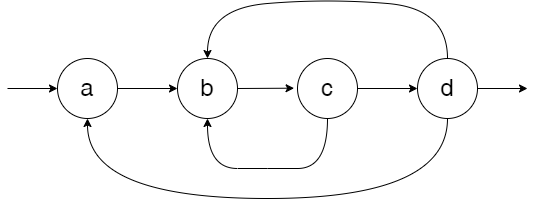
\includegraphics[width=0.9\linewidth]{includes/figures/LSTM.png}
    \caption{Grundidee einer LSTM-Architektur}
    \label{fig:diagram}
\end{figure}

Die Fähigkeit, Informationen zu sammeln erlaubt es gated \acp{RNN} Abhängigkeiten über
längere Zeiträume besser zu erlernen.


\subsection{Generative Modelle}
Generative Modelle, kurz \ac{GAN}, bilden eine Vielzahl von Algorithem ab,
welche für unsupervised learning genutzt werden. Sie bestehen aus einem Generator und einen
Diskriminator sowie einer Zielfunktion. Während der Generator versucht neue Daten zu
generieren und darauf trainiert wird, versucht der Diskriminator zu entscheiden, ob die ihm gegebenen
Daten echt sind, also aus der Trainingsmenge stammen, oder vom Generator generiert wurden.
Werden die Daten als generiert klassifiziert, muss sich der Generator anpassen und das Training
geht in die nächste Iteration.

Innerhalb der \ac{GAN}-Familie gibt es spezialisierte Varianten wie temporale Generative Adversarial Networks (tGANs) und Conditional Generative Adversarial Networks (cGANs):

\paragraph{Temporale Generative Adversarial Networks (tGANs)}
\ac{TGAN} sind zeitreihenoptimierte Modelle \cite{tgans_2021}. Sie berücksichtigen die zeitliche Abfolge und Muster in Daten, um realistische Zeitreihen zu generieren oder Informationen aus diesen zu ziehen, was sie ideal für Sensordatenprognosen macht.

\paragraph{Conditional Generative Adversarial Networks (cGANs)}
\ac{CGAN} fügen eine bedingte Komponente hinzu, die es ermöglicht, Daten basierend auf spezifischen Bedingungen oder Labels zu generieren \cite{AnIntrod85:online}. 
Sie sind daher interessant, wenn generierte Daten bestimmten Kriterien entsprechen müssen, wie beispielsweise bei der zielgerichteten Bildsynthese oder in spezialisierten medizinischen Anwendungen.
\chapter{Personas}
\label{cha:Personas}
Personas sind fiktionale Repräsentationen von Zielgruppen oder Nutzern, die deren Charakteristika, Verhalten und Bedürfnisse aufzeigen. 
Im \acl{UCD} dienen sie dazu, benutzerorientierte Lösungen zu entwickeln. Da sich Personas an den realen Nutzern orientieren, helfen sie Designern und Entwicklern, 
einen tieferen Einblick in ihre Zielgruppe zu gewinnen. Der dadurch entstehende Designprozess ist nutzerorientiert und ermöglicht die Bereitstellung von Lösungen, 
die dem Kunden oder Nutzer einen echten Mehrwert bieten. Des Weiteren erleichtern Personas die Kommunikation innerhalb von Teams\cite{Personas96:online}, indem sie als gemeinsamer Bezugspunkt 
dienen, Verwirrungen beseitigen und die Bemühungen aller Beteiligten aufeinander abstimmen. Oft wird im Erstellungsprozess deutlich, welche Punkte für den Nutzer besonders wichtig sind, was zu einer Priorisierungsreihenfolge führen kann.

\section{Fathima Olsson}
\subsection*{Hintergrund}
Fathima ist eine junge Medizintechnik-Studentin, die unter anderem im Bereich der Diabetes-Warngeräte forscht. Ihr Ziel ist es, die Fähigkeiten dieser Geräte zu erweitern. 
Da diese Geräte den Blutzuckerspiegel messen und den Nutzer warnen müssen, wenn dieser zu niedrig ist, muss das neue Gerät fehlerfrei funktionieren. Für die Validierung der 
Geräte sind umfangreiche Tests erforderlich, für die sie anonymisierte Testdaten mit Blutzuckerverläufen benötigt.

\subsection*{Demographie}
\personadetail{Geschlecht}{weiblich}
\personadetail{höchste Ausbildung}{Abitur}
\personadetail{Einkommen}{-}
\personadetail{Familienstand}{alleinstehend}
\personadetail{Sprachkenntnisse}{Deutsch, Englisch, Schwedisch}

\subsection*{Ziele}
\begin{itemize}
    \item Aufbau einer einfachen Testumgebung für schnelle und sichere Geräteentwicklung.
    \item Erweiterung der Fachkenntnisse im Bereich Qualitätskontrolle medizinischer Geräte.
\end{itemize}

\subsection*{Herausforderungen}
\begin{itemize}
    \item Beschaffung kostengünstiger und präziser Daten, die bedarfsgerecht angepasst oder erstellt werden können.
    \item Aufbau von Testszenarien, die auch kritische Werte simulieren können.
    \item Entwicklung eines sicheren und prüfbar funktionalen Konzepts zum Testen medizinischer Technologien.
\end{itemize}

\subsection*{Verhalten}
\begin{itemize}
    \item Forschungsorientierung: Fathima ist neugierig und motiviert, in ihrem Fachgebiet zu forschen und neue Erkenntnisse zu gewinnen.
    \item Präzision: Sie arbeitet genau und sorgfältig, insbesondere bei der Durchführung von Tests und Validierungen.
    \item Problemlösungskompetenz: Sie hat die Fähigkeit, komplexe Probleme zu analysieren und kreative Lösungen zu entwickeln.
    \item Zielorientierung: Ihr Ziel ist es, Menschen zu helfen, und sie ist bereit, die notwendigen Schritte zu unternehmen, um dies zu erreichen.
\end{itemize}

\subsection*{Bedürfnisse}
\begin{itemize}
    \item Einfache Nutzung: Das System muss einfach und flexibel einsetzbar sein.
    \item Nachnutzung eigener Daten: Die Software muss Möglichkeiten bieten, mit eigenen Daten zu arbeiten.
\end{itemize}

\subsection*{Zitat}
``Wenn es darum geht, Menschen in schwierigen Situationen zu helfen, darf man sich keine groben Fehler erlauben.``

\section{Dieter Maibach}
\subsection*{Hintergrund}
Dieter Maibach ist ein 50-jähriger Maschinenbau-Ingenieur, der vor etwa 30 Jahren studiert hat und seitdem in derselben Firma arbeitet. 
Er und seine Kollegen sind hauptsächlich für die Entwicklung neuer Mikrocontroller zuständig. Diese sind hochspezialisiert und müssen daher sehr stabil und zuverlässig laufen, 
weshalb sie eine umfangreiche Testsuite benötigen. Die Testsuite muss in der Lage sein, Signale, die von Sensoren an den Mikrocontroller gesendet werden, zu simulieren, 
um zu überprüfen, ob er richtig reagiert. Da das Ganze in einem großen Unternehmen stattfinden soll und frei zugänglich sein muss, muss die Anwendung frei zugänglich sein.

\subsection*{Demographie}
\personadetail{Geschlecht}{männlich}
\personadetail{höchste Ausbildung}{Hochschulabschluss}
\personadetail{Einkommen}{60.000}
\personadetail{Familienstand}{verheiratet}
\personadetail{Sprachkenntnisse}{Deutsch, Englisch (A1), Russisch}

\subsection*{Ziele}
\begin{itemize}
    \item Einführung von Qualitätsverbesserungsmethoden in den Entwicklungsprozess, um die Stabilität und Zuverlässigkeit der entwickelten Mikrocontroller zu steigern.
    \item Erweiterung der Fachkenntnisse im Bereich der Mikrocontroller-Entwicklung, um mit neuen Technologien und Designkonzepten auf dem neuesten Stand zu sein.
\end{itemize}

\subsection*{Herausforderungen}
\begin{itemize}
    \item Generierung von realistischen Testdaten und deren Konfiguration.
    \item Aufbau von Testszenarien, die auch kritische Werte simulieren können.
    \item Einführung von neuen Methoden/Tools in einen alten, lang bestehenden Entwicklungsprozess.
\end{itemize}

\subsection*{Verhalten}
\begin{itemize}
    \item Gewissenhaftigkeit: Dieter arbeitet präzise, genau und sorgfältig.
    \item Analytisches Denken: Er hat eine ausgeprägte Fähigkeit, komplexe Probleme zu analysieren und logische Lösungen zu finden.
    \item Innovationsfähigkeit: Dieter ist offen für neue Ideen und hat die Fähigkeit, kreative Lösungsansätze zu entwickeln.
    \item Beharrlichkeit: Er gibt nicht schnell auf und ist bereit, Herausforderungen anzunehmen und hartnäckig an Lösungen zu arbeiten.
    \item Teamorientierung: Dieter arbeitet gerne im Team und bringt einen kooperativen Ansatz ein.
\end{itemize}

\subsection*{Bedürfnisse}
\begin{itemize}
    \item Einfaches UI/UX Design: Die Software muss einfach zu bedienen und möglichst selbsterklärend sein.
    \item Einfache Bedienung: Die Software muss einfach in bestehende Umgebungen integrierbar sein.
    \item Flexible Nachnutzung: Testszenarien müssen im Team einfach nachnutzbar sein.
\end{itemize}

\subsection*{Zitat}
``Solange es zuverlässig und einfach ist, kann ich mich gerne mit neuen Sachen anfreunden.``

% !TeX program = xelatex

\chapter{Anforderungsanalyse der Software}

\section{Rückblick auf die originale Anwendung}
Um die Anforderungen an die neue und erweiterte Software zu verstehen, bietet es sich an ersteinmal sich den Ausgagspunkt der originalen Software anzuschauen.
Diese wurde als \acf{SPA} entwickelt. Sie besaß eine recht flache hierarchie und bildete die Datenstruktur des Backends ab. Das bedeutet, dass der Nutzer anstatt in verschiedenen Untermenüs zu navigieren, nur tiefer in die Beschreibung des \textit{Projects} eintaucht.
Dieses Vorgehen stellte sich al eine intuitive Lösung für den Nutzer heraus.


Zu beginn bekam der Nutzer direkt auf der Hauptseite eine Übersicht über alle \textit{Projects}, die er angelegt hat und die Möglichkeit neue Projekte anzulegen, zu bearbeiten, zu löschen oder hochzuladen (siehe Abbildung \ref{fig:old_mainpage_start}).
Ein Nutzeraccount an sich gab es nicht. Somit teilten sich alle Nutzer im Netzwerk die gleichen \textit{Projects}.

\begin{figure}[htbp]
    \centering
    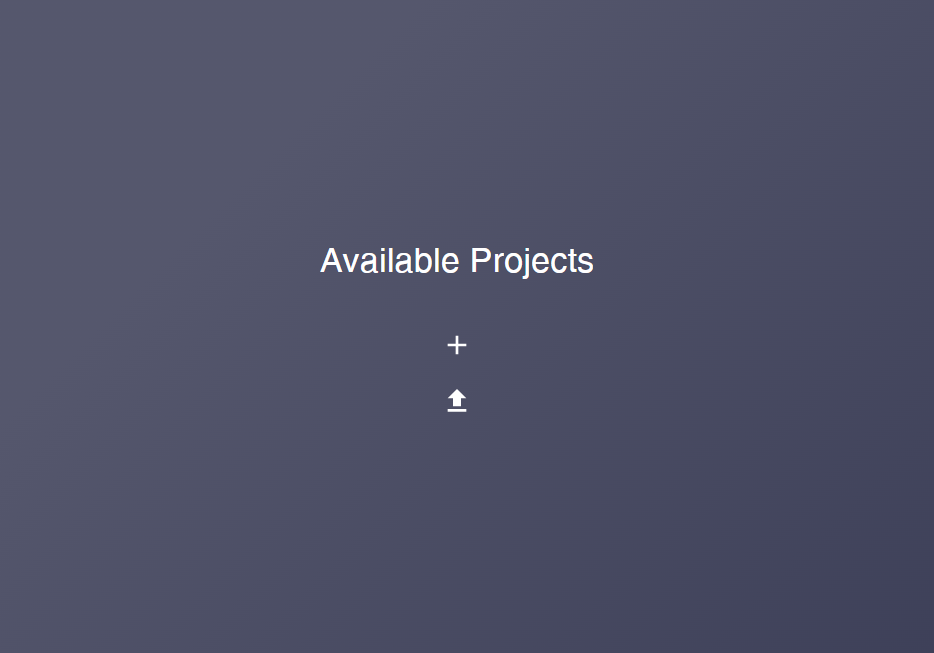
\includegraphics[width=0.9\linewidth]{includes/figures/old_version/ui_old_mainpage.png}
    \caption{Hauptansicht der originalen Anwendung, hier sind alle Projekte aufgelistet}
    \label{fig:old_mainpage_start}
\end{figure}

Um seine \textit{Projects} zu bearbeiten, muss der Nutzer auf den entsprechenden Button klicken und wird auf die Projektseite weitergeleitet. Dort findet sich eine Übersicht über alle vorhandenen \textit{Tracks}, 
Optionen diese zu bearbeiten und neue \textit{Tracks} anlegen. Auch finden sich innerhalb des \textit{Tracks} die einzelnen \textit{DataSets}, welche frei erstellt, bearbeitet, verschoben und gelöscht werden können (siehe Abbildung \ref{fig:dataset_old_version}).
Dies spiegelt die originale Datenstruktur wieder. Ein \textit{Project} besteht aus mehreren \textit{Tracks}, welche wiederum aus mehreren \textit{DataSets} bestehen. Die Abfolge wurde gewählt, damit Nutzer mehrere \textit{Track} parallel senden, 
und über die sukzessiv abgearbeiteten \textit{DataSets} die Struktur des im jeweiligen \textit{Tracks} definieren können.

\begin{figure}[htbp]
    \centering
    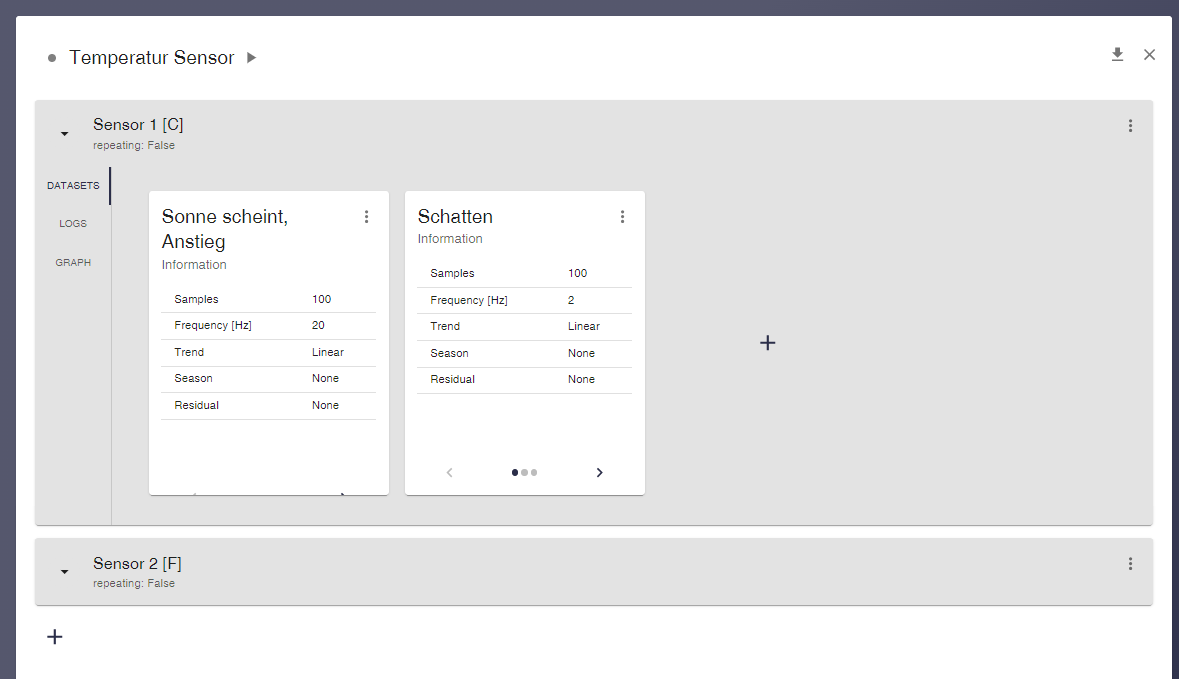
\includegraphics[width=0.9\linewidth]{includes/figures/old_version/ui_old_dataset.png}
    \caption{\textit{DataSet} Ansicht der originalen Anwendung}
    \label{fig:dataset_old_version}
\end{figure}

Das Senden der Daten erfolgt über einen entsprechenden Button, welcher, während gesendet wird, entsprechend der Abbildung \ref{fig:dataset_old_sending} innerhalb der \textit{Projects}-Seite und der Übersicht rot leuchtet und somit den Sendevorgang auch visuell bestätigt.

\begin{figure}[htbp]
    \centering
    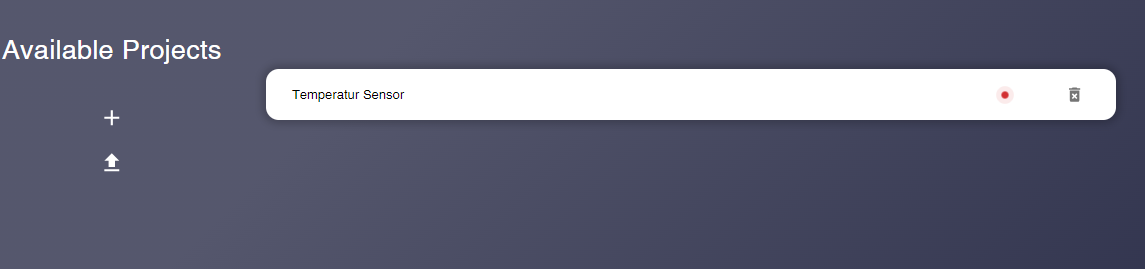
\includegraphics[width=0.9\linewidth]{includes/figures/old_version/ui_old_projects.png}
    \caption{\textit{DataSet} Ansicht der originalen Anwendung}
    \label{fig:dataset_old_sending}
\end{figure}

Themen wie Eingabenvalidierung und Fehlerbehandlung wurden in der originalen Version nur durch JsonSchema vorgenommen und nicht tiefer konzeptioniert.
Flexibilität der zu sendenden Datentypen gab es auch nicht. Aufbauend auf dem gegebenen Schema wurden Fließkommazahlen generiert und versendet.
Auch wurde angenommen, dass der Nutzer der englischen Sprache mächtig ist und die Eingabeanforderungen und Beschreibungen versteht.





\label{cha:Anforderungsanalyse}
Eine Software, welche sowohl Daten generieren, als auch anhand von Daten trainieren soll kommt mit einer vielzahl an Anforderungen.
Grundsätzlich ist Datengenerierung bereits komplexes Thema, aber hierfür wurde im Ursprünglichen Projekt bereits ein Konzept erstellt. Dieses muss nur um neue Funktionalität erweitert/vorhandene Konzepte angepasst werden.
Trainieren anhand von Daten benötigt aber ein eigenes Konzept. Um beide Systeme zusammenzuführen, muss grob auf 5 Punkte geachtet werden.

\begin{itemize}
    \item Datenmanagement
    \item Trainieren der Modelle
    \item Benutzerschnittstelle und Benutzererfahrung
    \item Sicherheit und Privatsphäre
    \item Technische Anforderungen
\end{itemize}

Neben diesen 4 Punkten müssen auch ein paar technische Anforderungen erfüllt werden.


\section{Anforderungen an die Software}
\subsection{Datenmanagement}
\label{cha:Anforderungsanalyse:Datenmanagement}
Ein großer und elementarer Teil der zu erstellenden Software wird es sein, Daten zu verwalten und in verschiedensten Elementen der Software zu verarbeiten. Hierfür bedarf es eines sinnvollen Konzepts, 
um die Anforderungen der Software formulieren zu können.

Das spätere System muss in der Lage sein, Daten aus unterschiedlichen Quellen mit verschiedenen Datenformaten effizient zu verarbeiten. Da es Ziel ist, Daten aus fremden Quellen im System zu verarbeiten, 
müssen vom System gängige Formate verarbeitet werden. Eine solche Flexibilität ermöglicht dem System eine einfache Benutzung und eine breite Anwendbarkeit in verschiedenen Szenarien und erleichtert dem Nutzer die Handhabung der Software. Für die Verarbeitung verschiedener Datenformate muss eine universelle Verarbeitungslogik 
entwickelt werden, die diese in ein für das System nutzbares Format konvertiert und, da Formate wie JSON und CSV flexibel sind, diese auf valide Inhalte überprüft. Effizienter Umgang mit großen Datenmengen ist ebenfalls wichtig, 
um die Ressourcen schwächerer Systeme nicht zu überlasten. Entsprechende Vorverarbeitungsschritte müssen vom System durchgeführt werden. Die Umsetzung dieser Funktionen erfordert ein visuelles Bestätigungswerkzeug, das die Auswirkungen der 
Datenmanipulation in Echtzeit anzeigt und so eine transparente und zugängliche Benutzererfahrung schafft. Zudem muss sichergestellt werden, dass ausgewählte Vorverarbeitungsschritte reversibel sind, sodass Nutzer die Möglichkeit haben, die 
Vorverarbeitung und ihre spezifischen Parameter zu speichern und zu einem späteren Zeitpunkt zu nutzen oder zu verändern.

Das gesamte Konzept des Datenmanagements muss zudem erweiterbar sein, um neue Funktionalitäten und Abhängigkeiten in Zukunft zu ermöglichen. Das Datenmodell muss daher Möglichkeiten bieten, um neue Datenformate und Vorverarbeitungsschritte zu 
integrieren. Während dies die Komplexität und den initialen Aufwand erhöht, wird es die Wartung und Erweiterung der Software in Zukunft erleichtern.


\subsection{Trainieren und Konfigurieren von Modellen}
\label{concept:training}
In der Anforderungsanalyse für das Training von \ac{ML} Modellen sowie Zeitreihenzerlegungs- und Analysealgorithmen liegt der Fokus auf der Entwicklung einer benutzerfreundlichen, effizienten und interaktiven Trainingsumgebung.
Da es nicht möglich ist, den richtigen Algorithmus für alle Anwendungsfälle zu finden, muss die Software eine Vielzahl von Algorithmen bereitstellen, die jeweils detailliert in Bezug auf ihre Eigenschaften und Anwendungsbereiche beschrieben werden.
Wesentlich ist hierbei eine intuitive Konfiguration aller Algorithmen, die auch für Benutzer ohne spezialisiertes Wissen in diesen Bereichen zugänglich ist. 
Gleichzeitig sollte eine Balance zwischen einfacher Bedienbarkeit und der Möglichkeit zur Feinabstimmung der Modelle gefunden werden, um eine breite Nutzerbasis zu bedienen.

Da das Training von Modellen eine rechenintensive Aufgabe darstellt, muss die Software eine effiziente Nutzung der Systemressourcen sicherstellen, um auch auf weniger leistungsfähigen Systemen eine reibungslose Funktion zu garantieren.
Dies ist wichtig, da die Infrastruktur der Software nicht nur auf leistungsstarken Servern, sondern auch auf lokalen Systemen mit begrenzten Ressourcen betrieben werden soll.

Abschließend ist die transparente Darstellung der Trainings- und Validierungsergebnisse entscheidend. Die Ergebnisse sollten schnell und effizient präsentiert werden und sich an unterschiedliche Benutzeranforderungen anpassen lassen. 
Dies gewährleistet, dass die Trainingskomponente der Software sowohl für Experten als auch für Laien geeignet ist, was die Zugänglichkeit und Effektivität der Software insgesamt steigert.


\subsection{Benutzerschnittstelle und Benutzererfahrung}
\label{cha:Anforderungsanalyse:Usability}

Die Gestaltung der Benutzeroberfläche der Software erfordert ein tiefgreifendes Verständnis für die Bedürfnisse und Erwartungen der Nutzer. 
Der Nutzer muss im Zentrum aller Designentscheidungen stehen, wobei das Ziel ist, eine Umgebung zu schaffen, in der sich die Benutzer sicher und kompetent in ihren Interaktionen fühlen und stets die Kontrolle über die Software behalten. 
Um dies zu erreichen, ist eine effiziente und benutzerfreundliche Oberfläche unerlässlich.

Gemäß der ISO 9241-110\footnote{Die ISO Norm 9241-110, auch als Grundsätze der Dialoggestaltung bekannt, behandelt die ergonomische Gestaltung von interaktiven Systemen und unterteilt diese in sieben Grundkonzepte.} lassen sich 
verschiedene grundlegende Anforderungen identifizieren, die für die Gestaltung einer effektiven Benutzeroberfläche wesentlich sind. Nachfolgend werden diese Anforderungen, basierend auf der Interpretation aus \cite{DieGrund14:online}, dargestellt:

\begin{description}
    \item[Aufgabenangemessenheit] Die Benutzeroberfläche sollte so gestaltet sein, dass Voreinstellungen von Standardwerten und die Struktur der Dialogwege die Aufgaben des Benutzers widerspiegeln und unterstützen.
    \item[Steuerbarkeit] Die Benutzer müssen die Möglichkeit haben, die Abfolge und Tiefe der angebotenen Dialoge nach ihren Bedürfnissen zu steuern.
    \item[Erwartungskonformität] Alle Aktionen und Steuerelemente in der Software sollten nachvollziehbar und konsistent mit den Erwartungen des Benutzers sein.
    \item[Selbstbeschreibungsfähigkeit] Die Software sollte Wartezeiten visualisieren, klare Links bereitstellen und bei Bedarf Hilfestellungen anbieten, um dem Benutzer stets Orientierung zu geben.
    \item[Lernförderlichkeit] Die Software sollte eine klare, logische und sinnvolle Strukturierung komplexer Aufgaben bieten, um eine einfache Erlernbarkeit zu gewährleisten.
    \item[Fehlertoleranz] Eingabefehler sollten angemessen behandelt werden, ohne dass die Software abstürzt, und der Benutzer sollte weiterhin in der Lage sein, seine Ziele zu erreichen.
    \item[Individualisierbarkeit] Die Software sollte es dem Benutzer ermöglichen, die Oberfläche und Funktionalitäten an seine individuellen Bedürfnisse anzupassen.
\end{description}

Eine weitere wichtige Anforderung ist die Bereitstellung von mehrsprachigkeit. Software, gerade wenn sie komplexe Themen aufgreift, sollte die mentale Leistung seiner Nutzer nicht unnötig belasten, indem man Fachthemen in einer Fremdsprache behandelt.
Dies kann zu Missverständnissen und Fehlern führen, die die Effektivität der Software beeinträchtigen. 
Die Berücksichtigung dieser Prinzipien stellt sicher, dass die Benutzeroberfläche nicht nur funktional und effizient ist, sondern auch ein angenehmes und effektives Benutzererlebnis bietet, 
das auf die Bedürfnisse und Fähigkeiten verschiedener Nutzergruppen zugeschnitten ist.




\subsection{Sicherheit und Privatsphäre}
Da es ein integraler Teil der Software sein wird, eigene Daten hochzuladen, diese zu speichern und zu verarbeiten, ist die Anforderung an einen vernünftigen Datenschutz und Datensicherheit notwendig. 
Um den Schutz dieser sensiblen Benutzerdaten zu gewährleisten, ergeben sich aus den folgenden rechtlichen Rahmenbedingungen spezifische Anforderungen.

Unter Berücksichtigung der EU-Datenschutz-Grundverordnung (DSGVO) müssen technische und organisatorische Maßnahmen implementiert werden, um ein angemessenes Schutzniveau für die 
Verarbeitung personenbezogener Daten sicherzustellen. Insbesondere Artikel 32 DSGVO fordert die Verschlüsselung und sichere Verarbeitung von Daten, um sie vor unbefugtem Zugriff zu schützen. Dies beinhaltet in diesem Fall auch den 
Schutz vor anderen Nutzern. Während die hochgeladenen Daten nicht zwangsläufig die Identifikation einer Person ermöglichen, können sie dennoch Daten enthalten, welche Rückschlüsse auf eine Person zulassen könnten. 
Beispielsweise können Sensordaten der Haussteuerung Rückschlüsse auf die Gewohnheiten und das Verhalten einer Person zulassen. Dies muss durch entsprechende Maßnahmen abgesichert werden. Hieraus ergibt sich aber auch eine technische Anforderung. 
Da es sich bei der Anwendung um eine Webanwendung handelt, müssen die gesamten Strukturen, die ein Nutzer pflegt, separiert werden. Hierfür ist ein entsprechendes Konzept zu entwickeln.

Zusammenfassend ist es von höchster Wichtigkeit, dass die Anwendung ein robustes Sicherheitssystem implementiert, welches den rechtlichen Anforderungen entsprechend die Privatsphäre sowie die Sicherheit der Benutzerdaten effektiv schützt.


\subsection{Technische Anforderung}
Da sich in eine Vielzahl von Komponenten in der Entwicklung der Software abzeichnet, ist eine präzise und effektive Kommunikation zwischen diesen Komponenten unerlässlich, 
um die Gesamtfunktionalität der Anwendung zu gewährleisten. Daher sind umfassende Dokumentationen für jede Komponente entscheidend. Diese sollten nicht nur die Funktionsweise der einzelnen Komponenten detailliert beschreiben, sondern 
auch die Kommunikationsprotokolle und Schnittstellen zwischen ihnen klar darlegen. Eine solche Dokumentation ermöglicht die entwicklung der Systemarchitektur vollständig zu verstehen und effizient damit zu arbeiten.

Ein weiterer wichtiger Aspekt ist die einheitliche Fehlerbehandlung über die APIs. Ein konsistenter Ansatz in diesem Bereich erleichtert es dem Frontend, Fehler schnell zu identifizieren, zu verarbeiten und in einer für die Nutzer 
verständlichen Weise zu kommunizieren. Diese Konsistenz in der Fehlerbehandlung ist entscheidend für die Benutzerfreundlichkeit und die Stabilität der Anwendung.

Zusätzlich ist die Implementierung von Überwachungssystemen von großer Bedeutung, um den Zustand der Anwendung kontinuierlich zu überprüfen und mögliche Probleme frühzeitig zu erkennen. Solche Systeme sollten in der Lage sein, schnell 
auf erkannte Fehler zu reagieren und geeignete Maßnahmen zur Fehlerbehebung einzuleiten oder entsprechende Stellen darüber zu informieren.

Abschließend spielt auch die Einfachheit des Deployments eine wesentliche Rolle. Die Bereitstellung und Inbetriebnahme der Anwendung sollte so unkompliziert wie möglich sein, um eine effiziente und reibungslose in Betriebnahme zu 
gewährleisten. Dies umfasst sowohl die Erstinstallation als auch die Durchführung fortlaufender Updates. Durch die Berücksichtigung dieser 
Anforderungen wird sichergestellt, dass die Software nicht nur ihre Kernfunktionen erfüllt, sondern auch hohe Nutzerzufriedenheit und geringe Wartungsaufwände bietet.



\subsection{Anforderungen an die Software}
Fässt man die in den vorherigen Kapitel gesammelten Anforderungen zusammen, ergibt sich folgende Liste an Anforderungen an die Software:
\begin{enumerate}
    \item \textbf{Vielseitige Datenintegration und Unterstützung mehrerer Datenformate:} Unterstützt verschiedene Datenquellen und Formate, um eine flexible Datenhandhabung zu gewährleisten.
    \item \textbf{Effiziente Datenübertragung, -validierung und Systemressourcennutzung:} Sorgt für schnelle und korrekte Datenverarbeitung sowie optimale Nutzung der Systemressourcen.
    \item \textbf{Benutzerorientierte Datenauswahl und -vorverarbeitung sowie Verwaltung:} Ermöglicht es Nutzern, Daten auszuwählen und vorzubereiten, einschließlich Qualitätsoptimierung und reversibler Vorverarbeitungsschritte.
    \item \textbf{Visuelles Feedback, Datenexploration und transparente Ergebnisdarstellung:} Bietet klare visuelle Darstellungen und Werkzeuge zur Datenexploration, um Benutzern das Verständnis der Daten und Ergebnisse zu erleichtern.
    \item \textbf{Sicherheit, Privatsphäre und sicherer Umgang mit Benutzerdaten:} Gewährleistet Datenschutz und sichere Datenverarbeitung, einschließlich Zugriffskontrollen und Datentrennung.
    \item \textbf{Trainieren der Modelle und Bereitstellung einer Vielzahl von Algorithmen:} Ermöglicht das Trainieren verschiedener Modelle und bietet eine breite Palette an Algorithmen mit Beschreibungen und Anwendungsbereichen.
    \item \textbf{Benutzerschnittstelle, Benutzererfahrung und intuitive Konfiguration der Algorithmen:} Stellt eine benutzerfreundliche Oberfläche und einfache Konfigurationsmöglichkeiten der Algorithmen bereit.
    \item \textbf{Dokumentation, Fehlerbehandlung, Überwachung und Deployment:} Umfasst eine umfassende Dokumentation, einen einheitlichen Ansatz zur Fehlerbehandlung, Überwachung der Anwendungsperformance und vereinfachtes Deployment.
\label{list:requirements}
\end{enumerate}

Auf grundlage der hier definierten Anforderungen lässt sich direkt eine grobe Struktur des Projektes ableiten, unabhängig von den genutzten Technologien. Dieses wird im folgenden Abschnitt erläutert.
Die gewählten Technologien und deren Umsetzung wird in den Kapiteln \ref{cha:Implementation} und \ref{cha:setup} erläutert.





\section{Konzeption der Software}
\subsection{Datenmanagementkonzept}
Um die Anforderungen an das Datenmanagement zu erfüllen, muss ein Konzept entwickelt werden, das die Integration, Validierung und Verarbeitung von Daten ermöglicht. Da das System eine Vielzahl an Daten und Formaten unterstützen soll, 
ist die Entwicklung einer Datenstruktur sinnvoll, die alle Formate abbilden kann. Eine geeignete Lösung wäre die Konvertierung der Originaldaten in ein systemkompatibles Array-Format, wie beispielsweise Listen, die in den meisten 
Programmiersprachen einfach und effizient verarbeitet werden können.

Da es sich um Dokumente handelt, ist eine angemessene Persistenzmethode erforderlich. Um dies mit der relationalen Struktur des ursprünglichen Projekts zu verbinden, bietet sich eine Separation oder Kombination an. PostgreSQL, eine relationale Datenbank, 
die JSON-Dokumente speichern kann, wäre hierfür eine geeignete Wahl. Formate wie JavaScript Object Notation (JSON), Comma Separated Values (CSV) oder binäre Array-Formate wie NumPy-Arrays unterstützen solche Strukturen. Werden diese durch eine universelle 
Verarbeitungslogik in ein nutzbares Format konvertiert, muss die Validierung dem Nutzer aussagekräftiges Feedback zu möglichen Fehlern geben.

Im Rahmen der Vorverarbeitung muss es Nutzern möglich sein, hochgeladene Daten durch eine Reihe von Transformationsschritten zu leiten, die zur Optimierung der Datenqualität und zur 
Erleichterung des Lernprozesses der Algorithmen unerlässlich sind. Zu diesen Schritten gehören die Normalisierung der Daten, um eine einheitliche Skala zu erreichen, die optionale Entfernung linearer Trends zur 
Hervorhebung stationärer Komponenten in Zeitreihen und die frei wählbare Reduktion des Datenvolumens durch gezielte Verfahren. Bei mit Zeitstempeln versehenen Daten müssen eventuelle Lücken adäquat behandelt werden.

Angesichts der Komplexität dieser Schritte ist es wichtig, dass Nutzer Rückmeldungen zu ihren Änderungen oder Konfigurationen erhalten. Visualisierungswerkzeuge wie dynamische Graphen oder interaktive 
Datenexplorationsschnittstellen spielen dabei eine Schlüsselrolle. Sie ermöglichen es Nutzern, komplexe Datentransformationsprozesse zu visualisieren und deren Einfluss auf die 
resultierenden Daten und deren Qualität zu verstehen. Werden die Konfigurationen getrennt von den Originaldaten gespeichert, stellt die Reversibilität der Aktionen kein Problem dar.

Neben den Trainingsdaten müssen auch andere Datenstrukturen erstellt werden, die alle Notwendigkeiten rund um die neuen und alten API-Bereiche abdecken, da das bestehende Datenmodell nicht in der Lage ist, 
diese neuen Abhängigkeiten abzubilden. Ziel des Datenmanagementmoduls ist es, eine robuste, nutzerzentrierte Plattform für die Datenaufbereitung zu schaffen, die den Weg für präzises und effektives maschinelles Lernen ebnet.


\subsection{Konzeption des Modelltrainings}
Wie in der Sektion \ref{concept:training} erörtert, müssen verschiedene Algorithmen mit spezifischen Eigenschaften und Fähigkeiten zur Verfügung gestellt werden. Die Benutzeroberfläche der Webanwendung muss daher eine Auflistung dieser Algorithmen bereitstellen, 
inklusive einer detaillierten Beschreibung ihrer Anwendungsbereiche und Leistungsmerkmale, um Benutzern eine informierte Auswahl zu ermöglichen, die ihren spezifischen Anforderungen und dem Kontext ihrer Daten gerecht wird.
Da sich die Software nicht nur an Informatiker richtet, ist dies extrem wichtig.

Die individuelle Konfiguration der Modelle stellt eine Herausforderung dar, da sie eine Balance zwischen Benutzerfreundlichkeit und der Flexibilität der Anpassung erfordert. Feinabstimmungen der Hyperparameter im Konfigurationsprozess
können die Komplexität des Modells erhöhen, die Verarbeitungszeit verändern und potenziell signifikante Auswirkungen auf das Ergebnis des trainierten Modells haben. Daher ist es notwendig, die Konfiguration der Modelle einfach zu gestalten, 
den Nutzer während des Prozesses über die Auswirkungen zu informieren und die Möglichkeit zu bieten, die Konfigurationen zu speichern und zu laden, um sie später wiederzuverwenden.

Um einen effizienten Betrieb der Software zu gewährleisten, muss das Training die Systemressourcen effizient nutzen und sollte möglichst unabhängig vom Haupt-Thread operieren. Um die Systemauslastung zu minimieren, kann eine eigene Implementierung der Modelle teilweise die bessere Lösung sein, 
da hier die Anzahl der Parameter auf niedrige Systemressourcen optimiert werden kann.

Der letzte wichtige Punkt ist die Echtzeitinformation für das Modelltraining sowie das transparente Darstellen von Trainingsergebnissen.
Um den ersten Punkt umzusetzen, muss die Software eine Möglichkeit bieten, den Trainingsprozess zu überwachen und die Ergebnisse in Echtzeit zu visualisieren. Hierfür wären Websockets eine geeignete Lösung, da sie eine bidirektionale Kommunikation zwischen Client und Server ermöglichen.
Die Umsetzung des zweiten Punktes ist etwas einfacher. Während des Trainings Daten über Laufzeit, Loss und weitere Metriken zu sammeln und zu speichern, bedarf lediglich einer hierfür passenden Datenstruktur. Die Visualisierung der Ergebnisse kann durch einen Auszug aus den generierten Daten erreicht werden.


\subsection{Konzeption der Benutzeroberfläche}
Die Gestaltung der bereits bestehenden Benutzeroberfläche basierte auf den etablierten Prinzipien von Ben Shneidermans 8 Golden Rules of Interface 
Design\footnote{Die 8 Golden Rules of Interface Design sind eine Sammlung von Richtlinien für die Gestaltung von Benutzeroberflächen, die von Ben Shneiderman entwickelt wurden.}, wobei eine starke Übereinstimmung mit den zuvor genannten Anforderungen besteht. 
Daher wird in dieser Konzeption eine erneute Aufzählung dieser Richtlinien vermieden.

Die bestehende Benutzeroberfläche wurde unter Verwendung von React und Material UI entwickelt, was ein kohärentes und ästhetisch ansprechendes Erscheinungsbild sicherstellt. 
Dieses Framework bietet bereits eine umfangreiche Palette an Komponenten und Funktionen, die den Grundprinzipien des User Interface Designs entsprechen und somit viele der erforderlichen Anforderungen abdecken.

Ein wichtiger Aspekt in der Gestaltung ist die Nachbildung der Datenstruktur der \ac{API}, die den Nutzer durch die entsprechenden Interaktionsschritte leitet. Diese strukturelle Herangehensweise soll in der neuen Konzeption beibehalten werden. 
Eine Möglichkeit, dies zu erreichen, ist die Generalisierung der bereits verwendeten Komponenten, sodass diese die benötigten Datenstrukturen als Parameter erhalten und somit flexibel an neue Anforderungen angepasst werden können.
Um den Nuzter sicher durch die Anwendung zu leiten, muss dafür nur noch eine entsprechende Navigationskomponente entworfen werden, welche den Nutzer verständlich durch die verschiedenen Bereiche der Anwendung führt, hierbei aber eine klare, struckturelle Trennung der einzelnen Gebiete gewährleistet.

In Bezug auf die Individualisierbarkeit der Software sind derzeit nur begrenzte Anpassungen geplant. Funktionen wie Sprachänderungen sind vorgesehen, um das Benutzererlebnis zu verbessern. Hier sollte daher eine sinnvolle Lösung gefunden werden, eine I18n Integration in das gesammtkonzpt einzuarbeiten.
Allerdings ist eine umfassende Personalisierung von Dialogen und Abläufen auf Nutzerebene über die grundlegenden Anforderungen der Software hinaus nicht vorgesehen. 
Diese Entscheidung basiert auf der Abwägung von Nutzen, Notwendigkeit und Zeitaufwand für die spezifischen Anforderungen der Software.


\subsection{Konzeption des Sicherheitskonzeptes}
Um den Datenschutz und die Datensicherheit gemäß den Anforderungen zu gewährleisten, ist die Integration eines Nutzerkontosystems in die Anwendung von grundlegender Bedeutung. Durch eine angemessene Zugriffskontrolle, die über das Nutzerkonto realisiert wird, lässt sich ein unbefugter Zugriff auf sensible Daten effektiv verhindern. 

Die Implementierung einer Verschlüsselung für entsprechende Datenfelder bildet eine zusätzliche Schutzschicht. Dabei muss evaluiert werden, inwieweit diese Sicherheitsmaßnahme über mehrere \ac{API}s hinweg und innerhalb einer gemeinsam genutzten Datenbank umsetzbar ist. Aufgrund der Herausforderungen, die eine direkte Separierung oder Isolation innerhalb einer relationalen Datenbank mit sich bringt, ist eine umfassende Zugriffskontrolle über die APIs unerlässlich. Dies erfordert ein Sicherheitskonzept, in dem die Datenbank sicher hinter den Strukturen der API positioniert und geschützt wird.

Dieses Konzept stellt sicher, dass der Zugang zu sensiblen Benutzerdaten strikt kontrolliert und gesichert wird, um sowohl die Privatsphäre der Nutzer als auch die Integrität und Vertraulichkeit der Daten zu gewährleisten.


\subsection{Konzeption der technischen Anforderungen}
Das Projekt wird mehrere APIs sowie ein Frontend umfassen, welches diese APIs integrieren muss. Für eine effiziente Zusammenarbeit und nahtlose Integration aller Komponenten sind bestimmte technische Anforderungen 
und die Umsetzung von Best Practices notwendig. Eine dieser Anforderungen ist die Erstellung einer OpenAPI Spezifikation\footnote{Die OpenAPI Specification ist ein Format zur Beschreibung von REST APIs.}, 
die für die APIs entwickelt werden muss. Diese Spezifikation ermöglicht es Dritten, die APIs zu verstehen und zu nutzen, und bietet einen umfassenden Einblick in die vorhandenen REST-Endpunkte. 
Sie liefert präzise Beschreibungen der erforderlichen Parameter und illustriert die erwarteten Antwortstrukturen.

Zur Vereinheitlichung der Fehlerstruktur der APIs ist ein einheitlicher Ansatz für die Fehlerbehandlung erforderlich. Dies umfasst nicht nur ein konsistentes Verhalten beim Auftreten von Fehlern, 
sondern auch ein einheitliches Format für das Versenden von Fehlercodes. Eine solche Standardisierung ermöglicht eine effiziente Fehlerverarbeitung und gewährleistet, dass Fehler dem Nutzer auf verständliche Weise kommuniziert werden.

Ein umfassendes Überwachungssystem ist für die Gewährleistung hoher Stabilität der Anwendung unerlässlich. Dieses System sollte in der Lage sein, den Zustand der Anwendung kontinuierlich zu überwachen und 
mögliche Probleme frühzeitig zu erkennen. Die Implementierung sollte sowohl die Überwachung und Zentralisierung als auch die Auswertung der Logs der einzelnen Komponenten beinhalten, ergänzt durch die Überwachung der Metriken jeder Komponente.

Um den Deploymentprozess der Anwendung zu optimieren, ist es notwendig, diesen so weit wie möglich zu automatisieren. Idealerweise sollte die Anwendung mit einem einzigen Befehl aufgesetzt werden können. 
In diesem Kontext bietet es sich an, das in der ursprünglichen Anwendung genutzte System, bestehend aus einer Pipeline und einem Docker Compose Skript, zu übernehmen und um alle notwendigen Schritte zu erweitern.
% !TeX program = xelatex

\chapter{Aufbau}
\label{cha:setup}
\section{Überblick über die Infrastruktur}
\label{sec:infrastruktur}
Die ursprüngliche Anwendung setzte sich aus einer RESTful-API und einer \acl{SPA} für das Frontend zusammen. 
Für die Entwicklung des Frontends kam React zum Einsatz, ein Framework zur Gestaltung von Benutzeroberflächen, das 2013 von Meta veröffentlicht wurde \cite*{TheHisto67:online}. 
Dieses Framework ermöglicht insbesondere die Wiederverwendung von Komponenten, den fundamentalen Bausteinen der Benutzerschnittstelle. Die Wiederverwendbarkeit und Erweiterbarkeit der 
Komponenten sind entscheidende Prinzipien in React. Ergänzend dazu bieten Bibliotheken wie \acl{MUI}, die in diesem Projekt verwendet wurden, eine Sammlung vorgefertigter Komponenten an.

Das Backend wurde unter Verwendung von Spring Boot konzipiert, einem Tool, das auf dem Spring-Framework basiert und 2014 eingeführt wurde \cite*{SpringBo22:online}. Spring Boot erleichtert die 
Erstellung autonomer Microservices, die in der Java Virtual Machine (JVM) laufen und mit einem integrierten Tomcat-Webserver sowie einer Konfiguration ausgestattet sind, 
die zahlreiche Komponenten des Spring-Ökosystems zusammenführt.

Für die Datenpersistenz kam PostgreSQL zum Einsatz, ein relationales Datenbanksystem, das eine verlässliche Datenspeicherung bietet. Um Signale zu versenden, wurde Kafka, eine verteilte Event-Streaming-Plattform, verwendet.

Die bestehende Infrastruktur, basierend auf einem Technologie-Stack aus React, Spring und PostgreSQL erfordert Erweiterungen, um die Integration von Machine Learning und Zeitreihenanalyse zu ermöglichen.

Wie in Abbildung \ref*{fig:setup} schematisch dargestellt, erfordert die Erweiterung des Projekts ein zusätzliches REST-Framework. Django, ein auf Python basierendes Webframework, 
das 2005 veröffentlicht wurde, soll in das System integriert werden und für das Training der Machine-Learning-Modelle verantwortlich sein.
Graylog wird erst durch die Einführung von Microservices notwendig und dient dazu, die Protokolle der verteilten Systeme zu erfassen.
Prometheus wird als Monitoring-Tool eingesetzt, um die Überwachung der jeweiligen Container zu gewährleisten.
Redis, ein Key-Value-Datenspeicher, ermöglicht Caching und den Betrieb von Multithreading-Operationen über Websockets.
Traefik fungiert als Reverse-Proxy und regelt die Kommunikation zwischen den verschiedenen Diensten bzw. Containern.

Das Ziel dieser neuen Container und Werkzeuge ist es, ein stabil laufendes und wartbares System zu schaffen.


\section{Microservice-Architektur}
Die Microservice-Architektur ist eine methodische Innovation in der Softwareentwicklung, die eine Anwendung in eine Kollektion von kleineren, unabhängigen Diensten aufspaltet. 
Diese Dienste, bekannt als Microservices, sind für spezifische Funktionen oder Geschäftslogiken verantwortlich und können unabhängig voneinander entwickelt, bereitgestellt und skaliert werden. 
Die Kommunikation zwischen diesen Diensten erfolgt über wohldefinierte Schnittstellen, meist RESTful APIs, die eine hohe Interoperabilität gewährleisten. 
Auch erlauben Microservices polyglotte Programmierung, dies bedeutet, dass Microservices in unterschiedlichen Sprachen und mit unterschiedlichen Technologien implementiert werden können.


Diese Art der Architektur steht im Kontrast zu monolithischen Systemen, in denen alle Komponenten einer Anwendung eng miteinander in einer einzigen Codebasis integriert sind. 
Monolithen bieten zwar Vorteile wie die Wiederverwendung von Code und eine einheitliche Entwicklungs- und Deployment-Umgebung, sie sind jedoch in Bezug auf Skalierbarkeit und Flexibilität limitiert. 
Skalierung ist bei Monolithen oft nur vertikal möglich, was bedeutet, dass man die Ressourcen eines einzelnen Servers erhöht, im Gegensatz zum horizontalen Skalieren bei Microservices, wo man die Last auf mehrere Server verteilen kann.

In diesem spezifischen Anwendungsfall ermöglicht die Microservice-Architektur eine sinnvolle Skalierbarkeit, indem beispielsweise Dienste für das Training von Machine Learning Modellen auf leistungsstarken Servern betrieben werden, 
während einfachere CRUD-APIs\footnote{CRUD-API bezieht sich auf eine \ac{API}, welche hauptsächlich für Datenbankoperationen zuständig ist} auf weniger leistungsfähigen Systemen laufen können. 
So könnte ein Django-Service für Machine Learning und Zeitreihenzerlegung zuständig sein, während ein Spring-Service sich auf das Erstellen und Versenden von Datenstreams konzentriert.

Die Flexibilität der Microservice-Architektur erleichtert zudem die Integration neuer Technologien und Ansätze. Da jeder Service unabhängig ist, können Innovationen in einem Service implementiert werden, ohne von bestehenden Systemen oder Technologiestacks beeinträchtigt zu sein. 
Dies fördert eine kontinuierliche Weiterentwicklung und Anpassung an neue Anforderungen.

Zusammenfassend bietet die Microservice-Architektur eine starke Grundlage für moderne, skalierbare und flexible Softwareentwicklungsprojekte. 
Sie unterstützt eine dezentralisierte Entwicklungsstrategie, die Anpassungen und Skalierungen erleichtert und dabei hilft, die technische Schuld zu minimieren, indem sie die Unabhängigkeit von Diensten gewährleistet.

\section{Technologie-Stack} 
\paragraph{Apache Kafka}
Apache Kafka, ein leistungsstarkes Open-Source-Stream-Processing-System, bildet das Herzstück dieses Projekts für die Verarbeitung von Datenströmen in Echtzeit. 
Es fungiert als zentrale Austauschplattform, die eine effiziente und zuverlässige Datenübertragung zwischen den Datenproduzenten (Producers) und den Datenkonsumenten (Consumers) ermöglicht. 
Somit kann die Datenübertragung der Signale, die zeitrelevant und kontinuierlich erfolgen muss, abgesichert und kann durch neue Consumer unabhängig auf verschiedenen Plattformen genutzt werden.

\paragraph{Docker}
\label{sec:docker}
Docker hat sich als eine transformative Technologie in der Welt der Softwareentwicklung etabliert, die es ermöglicht, Anwendungen in Containern zu verpacken. 
Diese Container sind leichtgewichtige, eigenständige Pakete, die alles enthalten, was eine Anwendung zum Laufen benötigt, von Umgebungsvariablen und Konfigurationsdateien bishin zu Code, Laufzeitumgebung und den genutzten Bibliotheken. 
Docker vereinfacht damit die Bereitstellung und den Betrieb von Anwendungen, indem es für Konsistenz über verschiedene Entwicklung, Release-Zyklen und Cloud-Umgebungen hinweg sorgt.

Der Einsatz von Docker im Projekt bietet entscheidende Vorteile: Es ermöglicht, dass das Projekt praktisch überall ausgeführt werden kann, unabhängig von spezifischen Hardwarekonfigurationen. 
Dies ist besonders nützlich in heterogenen Umgebungen, wo die Unterstützung verschiedener Betriebssysteme und Plattformen erforderlich ist. Docker ermöglicht auch eine erhebliche Skalierbarkeit, 
vor allem in Verbindung mit einer Microservice-Architektur. In solch einem Ökosystem kann Docker dazu beitragen, die Anwendungen leicht skalierbar und wartbar zu machen. 
Mit Docker können auch Aktualisierungszyklen beschleunigt werden, da neue Versionen schnell und automatisiert bereitgestellt werden können, was für 
kontinuierliche Integration und kontinuierliche Bereitstellung (CI/CD) von entscheidender Bedeutung ist. 
Auch ermöglichen Techniken wie Blue-Green-Deployment eine nahtlose Umschaltung zwischen verschiedenen Versionen der Anwendung, was das Risiko bei der Bereitstellung neuer Versionen minimiert.

Docker Compose ist ein Tool, das das Management von Multi-Container-Anwendungen vereinfacht. Mit einer einzigen Konfigurationsdatei können Entwickler die Dienste, Netzwerke und Volumes definieren, die für ihre Anwendung erforderlich sind. 
Dies ist ideal für Single-Host-Deployments, welches für die Anwendung vorerst vorgesehen ist, und bietet die Flexibilität, unterschiedliche Konfigurationen für Entwicklung und Produktion zu definieren. 
Docker Compose erleichtert auch das Starten, Stoppen und Neubauen von Diensten und die Skalierung von Containern.

Für größere Deployments bietet Docker Swarm eine native Cluster-Verwaltungsfunktionalität, die Docker-Hosts zu einem virtuellen Single-Host macht. 
Swarm nutzt die Docker-API, was bedeutet, dass jede Software, die bereits mit Docker funktioniert, ohne Anpassungen mit Docker Swarm verwendet werden kann. 
Es orchestriert die Container, die auf einer Gruppe von Hosts ausgeführt werden, und enthält Dienste wie Load Balancing, die Anfragen über die Knoten hinweg verteilen.

Insgesamt bietet Docker eine effiziente, skalierbare und sichere Lösung für die Verpackung und Ausführung von Anwendungen, 
die die Art und Weise, wie Software entwickelt und betrieben wird, revolutioniert hat. Mit seinen Tools und Ökosystemkomponenten ist Docker eine ausgezeichnete 
Wahl für moderne Softwareprojekte, die schnelle Iterationen und eine hohe Verfügbarkeit erfordern.



\paragraph{Graylog}
Graylog, ein zentrales Log-Management-Tool, dient als eine entscheidendes Tool in der Systemarchitektur.
Als Open-Source-Plattform konzipiert, ermöglicht Graylog die automatisierte Zentralisierung, Sammlung und Analyse von Log-Daten. 
Spezifisch im Projekt spielt Graylog eine kritische Rolle bei der Überwachung der Kommunikation zwischen verschiedenen APIs, dem Frontend und der Datenbank. 
Durch die zentrale Erfassung von Logs bietet Graylog Einblicke in Systemereignisse und unterstützt so die Fehlerdiagnose und Optimierung des Systembetriebs.

Graylog baut auf dem ELK-Stack auf, einer Kombination aus Elasticsearch, Logstash und Kibana, die eine effiziente Log-Aggregation, -Analyse und -Visualisierung auf Systemebene ermöglicht. 
Der ELK-Stack wird häufig für umfassende Logging-Lösungen verwendet, wobei Graylog eine alternative Schnittstelle bietet, die auf ähnlichen Technologien basiert 
und darauf ausgerichtet ist, die Handhabung und Verarbeitung von Log-Daten zu vereinfachen.

Die Einrichtung eines zentralen Log-Management-Tools wie Graylog ist entscheidend für die Aufrechterhaltung der Systemintegrität, besonders in einer 
komplexen Microservice-Architektur. Durch die Konsolidierung der Logs an einem zentralen Punkt erleichtert Graylog das Monitoring und die Analyse von 
verteilten Systemen, was bei der Fehlersuche, Leistungsoptimierung und Sicherheitsüberwachung unerlässlich ist. Mit seinen leistungsstarken Such- und Analysefähigkeiten 
hilft Graylog Entwicklern und Systemadministratoren, schnell auf Ereignisse zu reagieren und die Systemstabilität zu gewährleisten.


\paragraph{Prometheus}
Im Jahre 2012 stellte Soundcloud mit Prometheus ein bedeutendes Werkzeug für das Monitoring und Alerting vor, das seither insbesondere in großen und verteilten 
Systemen breite Anwendung findet. Das Tool ist spezialisiert auf die Sammlung, Speicherung und das Management von Metriken in Zeitreihenform. 
Diese Fähigkeit ist entscheidend, um einen Überblick über die Gesundheit und Leistung der überwachten Systeme zu erhalten. 
Bei auftretenden Anomalien ist Prometheus so konzipiert, dass es Warnmeldungen auslöst, um auf potenzielle Probleme hinzuweisen\cite*{Overview70:online}.

In Bezug auf dein aktuelles Projekt ermöglicht Prometheus eine zentralisierte Überwachung der einzelnen Systemkomponenten, wodurch eine sofortige und präzise 
Diagnose bei Performance-Einbußen oder Ausfällen einzelner Teile des Systems ermöglicht wird. Durch die Analyse der erfassten Daten lassen sich nicht nur kurzfristige 
Zustände und Fehlfunktionen erkennen, sondern auch langfristige Muster und Trends, die Rückschlüsse auf die Effizienz und Angemessenheit der zugrunde liegenden 
Infrastruktur zulassen.




\paragraph{Traefik}
Traefik, ein moderner HTTP-Reverse-Proxy und Load Balancer, wurde speziell für Microservice-Architekturen und deren dynamische Anforderungen entwickelt. 
Er zeichnet sich durch eine automatische Systemerkennung und Konfiguration aus, was ihn zu einem unverzichtbaren Werkzeug für die reibungslose Verwaltung von 
Netzwerkanfragen in komplexen Systemen macht. Traefik integriert sich nahtlos mit etablierten Infrastrukturkomponenten wie Docker, Docker Compose und Docker Swarm, 
wodurch die Verteilung von Anfragen auf die entsprechenden Services vereinfacht wird.

Durch seine intuitive Konfiguration und automatische Serviceerkennung entlastet Traefik Entwickler von manuellen Setup-Prozessen und fördert eine effiziente 
Bereitstellung von Services. Darüber hinaus bietet Traefik Echtzeit-Einblicke in das Netzwerkverhalten und unterstützt Let's Encrypt für die Automatisierung 
von SSL/TLS-Zertifikaten, was die Sicherheit erhöht. Durch seine Fähigkeit, dynamisch auf Änderungen in der Service-Landschaft zu reagieren, ist Traefik ein 
essentielles Element in der Toolchain für die Implementierung und den Betrieb von Microservices, das Leistungsfähigkeit mit Benutzerfreundlichkeit vereint.


\paragraph{PostgreSQL}
PostgreSQL ist ein fortschrittliches Open-Source-Datenbanksystem, das für seine Robustheit, Flexibilität und Compliance mit SQL-Standards bekannt ist. 
Es bietet erweiterte Funktionen, wie komplexe Abfragen, Fremdschlüssel, Trigger, updatable Views und Transaktionen mit hoher Integrität. PostgreSQL eignet sich 
besonders gut für Aufgaben, die komplexe Datenverarbeitungen erfordern und bei denen die Datenkonsistenz von höchster Wichtigkeit ist. 
Die Architektur unterstützt sowohl relationale als auch JSON-Datentypen, was es zu einer vielseitigen Wahl für vielfältige Anwendungsfälle macht.

\paragraph{Redis}
\label{sec:redis}
Redis ist ein Open-Source-Key-Value-Datenspeicher, der für seine Geschwindigkeit, Flexibilität und Vielseitigkeit bekannt ist. 
Es ist ein NoSQL-Datenspeicher, der Daten in einem Schlüssel-Wert-Format speichert und eine Vielzahl von Datenstrukturen unterstützt, darunter Strings, Hashes, Listen, Sets und geordnete Sets.
Redis ist besonders gut für Anwendungen geeignet, die eine hohe Leistung erfordern, da es die Daten im Arbeitsspeicher speichert und so eine schnelle Datenverarbeitung ermöglicht. Im aktuellen Projekt wird Redis für Websockets eingesetzt.


\paragraph{Gitlab CI und Gitlab Runner}
Gitlab bietet über eigene, sogenannte Pipelines, die Möglichkeit kontinuierlich Software zu testen und auszurollen.
Dank \acf{CICD} kann der auf Gitlab hochgeladene Code gebaut, getestet und, je nach Konfiguration des dafür eigens angelegten .gitlab-ci Files, deployed werden.
Es ist ein hilfreiches Tool um die Qualität der Software aufrecht zu erhalten und darüber hinaus ständig eine funktionierende Version aufrufbar zu haben.

\paragraph{Hugo}
\label{par:hugo}
Hugo ist ein Open-Source-Static-Site-Generator, der 2013 von Steve Francia veröffentlicht wurde. Er erlaubt das Erstellen von statischen Webseiten, die aus Markdown-Dateien generiert werden.
Somit lässt sich eine einfach und schnelle Dokumentation erstellen, die zudem noch leicht zu pflegen ist. In kombination mit einen Nginx\footnote{Nginx ist ein Webserver, der sich durch seine hohe Performance auszeichnet. Er dient hier als static file Server.} 
kann die Dokumentation auf einem Server gehostet werden und somit direkt an das Gesammtproject angebunden werden.


\begin{figure}[h]
    \centering
    \includegraphics[width=1.1\linewidth]{includes/figures/system_overview.png}
    \caption{Aktuelle Infrastruktur, sie verbindet das Frontend mit beiden APIs, welche Zugriff auf die PostgreSQL Datenbank haben. Überwacht werden sie von Prometheus und Graylog. Ein Kafka Producer wird genutzt um die genierierten Daten als Streams an entsprechende Consumer zu senden. Redis dient als Cache für die Websockets des Django-Channel Frameworks. Hugo wird genutzt um die Dokumentation zu generieren und über Nginx verfügbar zu machen. Dies alles  wird in Docker Containern ausgeführt.}
\label{fig:setup}
\end{figure}


\section{Zusammenfassung}
In diesem Kapitel wurde kurz die Architektur des Projekts präsentiert um dieses in einem produktiven Betrieb effizient nutzen zu können.
Hierbei wurde auf die Wahl einer Microservice-Architektur eingegangen und die einzelnen Komponenten vorgestellt. 
Es exiszieren somit neben den normalen Komponenten wie Front- und Backend auch Elementen, die sich um das Datenmanagement kümmern, wie PostgreSQL, Kafka und Redis.
Um die Anwendung zu überwachen und zu warten, werden Prometheus und Graylog eingesetzt. Wichtig für die flexible Inbetriebnahme sind die Komponenten aus dem DevOps Bereich, wie Docker, Docker Compose und Traefik.
Damit diese Schritte automatisiert werden können, wird Gitlab CI und Gitlab Runner eingesetzt. Zur Darstellung der Dokuemntation dient Hugo, neben der OpenAPI und Swagger Dokuemntation.

All diese Elemente sollten helfen, die Anwendung zuverlässig und stabil zu betreiben und die Wartungskosten zu minimieren.

% !TeX program = xelatex
\chapter{Implementation}
\label{cha:Implementation}


\section{Überblick}

Wie bereits in den vorherigen Kapiteln kurz angeschnitten muss die Software an vielen verschiedenen Punkten erweitert und, gerade im Bereich des maschinellen Lernens und der Zeit Serien Analyse, neu implementiert werden.
Da das Projekt aus 4 Teilen besteht, wird jedes Thema in einem der folgenden Kapitel separat erläutert.

In den jeweiligen Kapiteln werden sehr grob die Schritte gezeigt, welche für die jeweilige Implementierung notwendig waren. 
Auch wird auf spezifische Designentscheidungen eingegangen, welche für die jeweilige Implementierung notwendig waren und warum sich für gewisse Technologien entschieden wurde.



% !TeX program = xelatex
\section{Java Spring Boot}
Das Backend in Spring-Boot bildet das Herzstück der ursprünglichen Software. Es stellt eine vollständige API für das Frontend bereit, bindet die PostgreSQL-Datenbank ein und kommuniziert mit den Kafka-Brokern. 
Ursprünglich handelte es sich um eine "CRUD-ähnliche" API, die neben den grundlegenden CRUD-Operationen auch das Starten und Stoppen von Projekten ermöglichte.

Da die Software jedoch noch auf Spring Boot 2.7.5 lief und daher den Übergang von JavaX zu Jakarta nicht vollzogen hatte, mussten zuerst alle Maven-Abhängigkeiten aktualisiert werden. Zudem war das Frontend noch Teil der Maven-Ziele. 
Da die Anwendungen jedoch separat voneinander ausgeführt werden müssen, musste dies ebenfalls entfernt werden.

Basierend auf der Anforderungsanalyse aus Kapitel \ref{cha:Anforderungsanalyse} werden hier drei der fünf vorgestellten Punkte behandelt. Da es sich um die erste API handelt, die lediglich erweitert wurde, waren viele der 
technischen Anforderungen bereits erfüllt. Die Einführung von Metriken für Prometheus und ein zentralisiertes Logging wurde mithilfe entsprechender Bibliotheken, Konfigurationsdateien und Annotationen schnell umgesetzt.

\subsection{Architekturentscheidung und Umstrukturierung}
Um die Architektur der Software flexibler zu gestalten, war eine Umstrukturierung in Richtung einer hexagonalen Architektur wichtig. Diese Architektur stellt eine Erweiterung der von Eric Evans in "Domain-Driven Design: 
Tackling Complexity in the Heart of Software" \cite{evans2004ddd} beschriebenen Domain-Driven-Architektur dar. Diese vierschichtige Architektur unterscheidet sich in einigen wesentlichen Aspekten von den zuvor genutzten Strukturen, 
in denen Pakete streng nach Entitäten strukturiert wurden und sowohl Datenbank-, Service- als auch Kommunikationsschichten integriert waren. Dies reflektierte das übliche Domain-Driven Design, bei dem Anwendungen in Präsentations-, 

Logik- und Datenschichten unterteilt werden, um "Concerns", also Aufgaben, getrennt voneinander zu behandeln. Beispielsweise darf nur die Logik-Schicht Änderungen an den Daten vornehmen, während die Datenbankschicht lediglich zum Schreiben und 
Lesen genutzt wird. In der ursprünglichen Architektur war dies jedoch nicht konsequent umgesetzt, und es gab viele Überschneidungen.

Um die Trennung der Zuständigkeiten konsequent umzusetzen, war eine Umstrukturierung erforderlich. Da bereits zu Beginn klar war, dass die Spring-API auch mit anderen Services kommunizieren muss, bot sich eine hexagonale Architektur an. 
Das Ziel der hexagonalen Architektur, auch bekannt als "Ports-und-Adapter-Pattern", besteht darin, die Trennung zwischen der Logikschicht und den externen Schichten zu verstärken und zu konkretisieren. Dies geschieht, indem Akteure über 
technologieagnostische Schnittstellen wie Interfaces kommunizieren. Diese "Ports" dienen daher als Schnittstellen zwischen den Schichten. Die Adapter sind die Initiatoren der Interaktionen, beispielsweise RestController, JPARepositories oder 
WebsocketController, die als Schnittstellen nach außen agieren.


%% caption \caption{Links ist die alte Datenstruktur, rechts die neue}
\begin{figure}[htbp]
    \centering
    \begin{minipage}{.48\textwidth}
        \adjustbox{valign=t}{
            \begin{forest}
                for tree={
                font=\ttfamily,
                grow'=0,
                child anchor=west,
                parent anchor=south,
                anchor=west,
                calign=first,
                edge path={
                        \noexpand\path [draw, \forestoption{edge}]
                        (!u.south west) +(7.5pt,0) |- node[fill,inner sep=1.25pt] {} (.child anchor)\forestoption{edge label};
                    },
                before typesetting nodes={
                        if n=1
                            {insert before={[,phantom]}}
                            {}
                    },
                fit=band,
                before computing xy={l=15pt},
                }
                [de.tudresden.sus
                    [project
                            [ProjectController.java]
                            [ProjectService.java]
                            [Project.java]
                    ]
                    [track
                            [TrackController.java]
                            [TrackService.java]
                            [Track.java]
                    ]
                    [dataSet
                            [DataSetController.java]
                    ]
                ]
            \end{forest}
        }
    \end{minipage}\hfill
    \begin{minipage}{.48\textwidth}
        \adjustbox{valign=t}{
            \begin{forest}
                for tree={
                font=\ttfamily,
                grow'=0,
                child anchor=west,
                parent anchor=south,
                anchor=west,
                calign=first,
                edge path={
                        \noexpand\path [draw, \forestoption{edge}]
                        (!u.south west) +(7.5pt,0) |- node[fill,inner sep=1.25pt] {} (.child anchor)\forestoption{edge label};
                    },
                before typesetting nodes={
                        if n=1
                            {insert before={[,phantom]}}
                            {}
                    },
                fit=band,
                before computing xy={l=15pt},
                }
                [de.tudresden.sus
                    [adapter
                            [inbound
                                    [rest]
                                    [error]
                                    [websocket]
                            ]
                            [outbound
                                    [repositories]
                                    [entities]
                                    [mapper]
                            ]
                    ]
                    [ports]
                    [service]
                ]
            \end{forest}
        }
    \end{minipage}
    \caption{Alte Datenstruktur (links) und neue (rechts)}
\end{figure}


Die Vorteile dieser Architektur sind vielfältig: Sie fördert die Entkopplung von Komponenten, vereinfacht Tests, ermöglicht eine flexiblere Entwicklung durch die ausschließliche Implementierung gegen Interfaces und 
zeigt eine hohe Anpassungsfähigkeit gegenüber Änderungen. Ein potenzieller Nachteil könnte in der erhöhten Komplexität liegen, die jedoch durch das Weglassen der Domain-Modelle stark reduziert wurde.

Die neu definierten Schichten haben klare und abgegrenzte Verantwortlichkeiten. Das Adapter-Layer fungiert als oberste Schicht und beinhaltet alle externen Funktionalitäten. Es wird in einen Inbound- und einen Outbound-Teil 
unterteilt: Der Inbound-Teil ist verantwortlich für alle eingehenden Anfragen wie REST-Requests oder WebSocket-Verbindungen. Der Outbound-Teil umfasst alle nach außen gerichteten Funktionen, z.B. die Datenbankkommunikation oder 
den RestClient. Die Unterscheidung zwischen Inbound- und Outbound-Adaptern wird vom Datenfluss innerhalb des Service Layers gesteuert. Adapter, die Daten in das Layer eingeben und somit steuern, gehören zu den Inbound-Objekten. Adapter, 
die nach außen gehen, also vom Service Layer angesprochen werden, gehören in den Outbound-Bereich.

Im Port-Layer erfolgt die Kommunikation zwischen den Schichten. Anstatt eines direkten Zugriffs der RestController auf die Service-Beans wird ein Interface bereitgestellt, wobei Spring die korrekte Bean injiziert. 

Dies mag zunächst überflüssig erscheinen, entspricht jedoch dem Prinzip der Dependency Inversion: Höherrangige Komponenten sollten nicht direkt auf niederrangigere zugreifen, sondern lediglich auf deren Abstraktionen. Dies ermöglicht die 
flexible Austauschbarkeit verschiedener Implementierungen des Interfaces und erleichtert das Testen. Auch können Komponenten einfach ausgetauscht werden, ohne Einfluss auf die darunterliegende Struktur zu nehmen. So kann beispielsweise die 
REST-Schnittstelle komplett durch Websockets ersetzt werden, wobei nur die jeweiligen Endpunkte implementiert werden müssen. Die Geschäftslogik bleibt davon unberührt. Ebenso kann die verwendete Datenbank problemlos ausgetauscht werden, da ihre Schnittstelle 
durch das jeweilige Datenbank-Interface abstrahiert wird.

Obwohl viele hexagonale Architekturen ein Domain-Layer enthalten, der Domain-Modelle mit erweiterter Funktionalität gegenüber den Datenbankmodellen enthält, wurde in diesem Projekt auf dieses Layer verzichtet. Dies wurde gemacht, da es eine unnötige 
Komplexität eingeführt hätte und aktuell nicht notwendig erscheint. Die erforderlichen Funktionalitäten werden bereits durch bestehende Mapper-Klassen abgedeckt.


\subsection*{Anpassung der Datenstrucktur}
%% TODO: Datenstruktur anpassen
Ein Umbau der Datenstruktur, wie sie bereits in \ref{cha:Anforderungsanalyse:Datenmanagement} angedeutet wurde, lässt sich in zwei wesentliche Teile aufteilen.
\subsubsection{Datensätze und Vererbung}
Ursprünglich verfügte die Anwendung über eine recht einfache und sehr lineare Datenstruktur, welche im folgenden ER-Diagramm in Abbildung \ref{fig:datamodel_old_version} gezeigt wird.

\begin{figure}[ht]
    \centering
    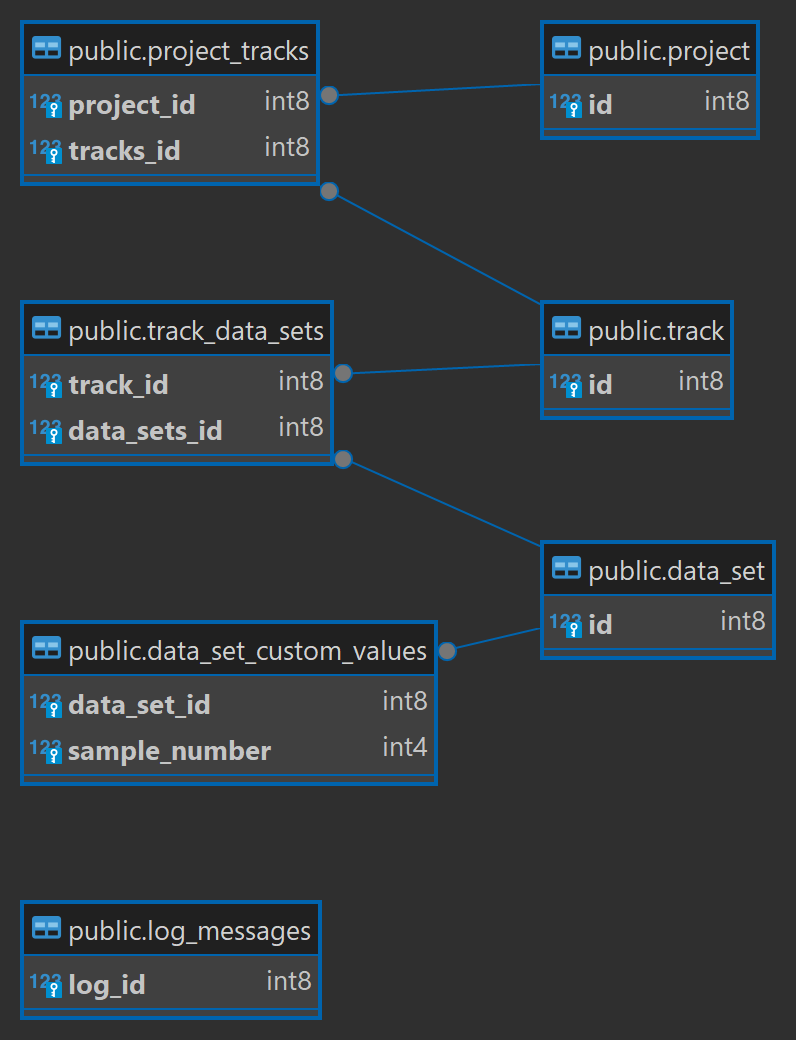
\includegraphics[width=1\textwidth]{includes/figures/database/software_old.png}
    \caption{Entity-Relationship-Diagramm der ursprünglichen Datenstruktur}
    \label{fig:datamodel_old_version}
\end{figure}



Diese Struktur bestand aus vier Komponenten: Ein Project ist in einer 1:n-Relation zu einem Track, der wiederum eine 1:n-Relation zu einem Datensatz hat. 
Diese Datenstruktur wurde ausgewählt, um komplexe Systeme modellieren zu können. Ein Project dient hierbei als Komponente, die mehrere datensendende Einheiten, 
sogenannte Tracks, umfasst. Da diese Tracks in unterschiedlichen Intervallen und insbesondere parallel senden können, war eine solche Unterscheidung notwendig. 
DataSets, aus denen ein Track besteht, fungieren als Abstraktionsebene der verschiedenen Phasen, in denen sich ein Track befinden könnte. So lassen sich durch aufeinanderfolgende DataSets unterschiedliche Situationen abbilden, 
beispielsweise die Simulation eines Gewächshauses (Project) mit drei Sensoren (Tracks) für Luftfeuchtigkeit, Temperatur und Lichtintensität. Die variierenden Bedingungen im Tagesverlauf, wie steigende und fallende 
Temperaturen, werden durch aufeinanderfolgende DataSets dargestellt. Jeder Track kann dabei eine eigene Frequenz besitzen.

Zur Nachverfolgung gesendeter Daten wird zudem ein Logverzeichnis angelegt.

Diese Herangehensweise erwies sich zwar als robust, jedoch auch als wenig flexibel. Die Art der zu sendenden Daten ließ sich nicht einfach anpassen, und die Zuweisung spezieller Eigenschaften zu unterschiedlichen 
Datentypen war nicht möglich. Die Beschränkung auf die in Trend, Residual und Season unterteilte Berechnungsvorschrift stellte eine weitere Limitierung dar.

Die erforderliche Flexibilität für die Erstellung komplexer Simulationsumgebungen und die Integration externer Konfigurationen, wie sie die Django-API ermöglicht, machte eine methodische Änderung notwendig. 

Hierfür wurden zwei Ansätze verfolgt:

\paragraph{Vererbung} 

Gemäß der in Listing \ref*{code:javaBaseDataSets} dargestellten Methode können neue Datensätze einfach von der Basisklasse erben. Neue Felder werden im selben Table gespeichert, wobei bei vielen neuen Feldern 
idealerweise eine neue Entität oder Entitätenstruktur erstellt werden sollte. Beim Auslesen aus der Datenbank wird dann über Casting die gewünschte Klasse rekonstruiert.
\begin{lstlisting}[language=Java, caption=Abstrakte Basisklasse der \textit{DataSets}, label={code:javaBaseDataSets}]
@Entity
@Inheritance(strategy = InheritanceType.SINGLE_TABLE)
@Accessors(chain = true)
@Data
@JsonTypeInfo(
        use = JsonTypeInfo.Id.NAME,
        include = JsonTypeInfo.As.PROPERTY,
        property = "type")
@JsonSubTypes({
        @JsonSubTypes.Type(value = CharDataSet.class, name = "char"),
        ...
})
@JsonAutoDetect(fieldVisibility = JsonAutoDetect.Visibility.ANY)
public abstract class PlainData implements DataTypeOption {

    @Id
    @Column(name = "id")
    @GeneratedValue(strategy = GenerationType.AUTO)
    private Long id;
    @Column(name = "position")
    private int position;
    @Column(name = "numSamples")
    private int numSamples;
    @Column(name = "frequency")
    private float frequency;
    @Column(name = "name")
    private String name;
    @Column(name = "dataType")
    private DataTypes dataType;
    ....
}
\end{lstlisting}


%% TODO neue DataSets einfügen und kurz erklären.


\paragraph{Polymorphe Deserialisierung} Um eine flexible Kommunikation zu gewährleisten, wird Jacksons polymorphe Deserialisierung eingesetzt\footnote{Jackson bietet eine umfangreiche Java API zum Arbeiten mit JSON}. Diese nutzt die in den 
\textit{@JsonSubTypes} definierten Optionen für das zielgerichtete Casting in die korrekten Objekte. Somit können die Objekte unabhängig vom Datentypen im Business-Layer verarbeitet werden und Typgerecht in der Datenbank gespeichert werden.

\begin{lstlisting}[language=Java, caption=Basisklasse der DTO Objekte, label={code:javaBaseDataSetsDTO}]
@JsonTypeInfo(
    use = JsonTypeInfo.Id.NAME,
    include = JsonTypeInfo.As.PROPERTY,
    property = "type")
@JsonSubTypes({
    @JsonSubTypes.Type(value = CharDataSetDTO.class, name = "char"),
    ...
})
@Data
@Accessors(chain = true)
@JsonAutoDetect(fieldVisibility = JsonAutoDetect.Visibility.ANY)
public class PlainDataDTO {

    @Schema(name = "id", nullable = true, minimum = "1")
    private Long id;
    ...
    
}
\end{lstlisting}


Jede Klasse muss außerdem eine eigene Mapper-Klasse bereitstellen, um die Datenstrukturen adäquat in die gewünschten DTOs zu konvertieren.

Die Implementierung dieser drei Klassen und ihrer Konfigurationen in den Basisklassen ermöglicht eine schnelle Erweiterung der bestehenden Datenstruktur. Zusätzlich implementieren alle Klassen ein Interface, das ihr jeweiliges Verhalten definiert. 
Dadurch kann eine neue Datenstruktur implementiert werden, ohne das Business-Layer zu beeinflussen. Wichtig ist, dass dieses Vorgehen den Grundsatz der Separation of Concerns nicht verletzt, da die neuen Datentypen lediglich eigene Datengenerierungsstrategien
implementieren, ohne das Verhalten außerhalb zu beeinflussen. Eine Ausnahme bilden die MLDataSet und TSADataSet, die ihre Daten extern (von der Django-API) beziehen. Hier wäre es theoretisch möglich, innerhalb der Entitäten einen REST-Client zu implementieren, 
was jedoch einen ungünstigen Datenfluss zur Folge hätte. Diese Aufgabe gehört eher zur Business-Logik und wird daher dort verarbeitet. Eine alternative Lösung wäre das Hinzufügen einer Domain-Schicht, die DataSets auf ein DomainModel projiziert. Da dies jedoch den 
Code unnötig aufblähen und bei den meisten DataSets diese Komplexität oder Abstraktion nicht benötigt wird, übernimmt das Business-Layer direkt diese Aufgabe.



\begin{lstlisting}[language=Java, caption={Mapper Klasse für DataSets, basierend auf den dataType, ein separates enum, fügen die Datentype eigenen mapper ihre Felder hinzu, bevor die global gültigen Felder gefüllt werden.}, label={code:javaBaseDataMapping}]
private final CharDataSetMapper stringMapper;
private final FloatDataSetMapper floatMapper;
private final IntegerDataSetMapper intMapper;
private final MlDataSetMapper mlMapper;
private final TSADataSetMapper tsaMapper;
private final CustomValueConverter customValueConverter;
private final SleepDataSetMapper sleepMapper;

public PlainData toEO(PlainDataDTO data) {
    var eo =  switch (data.getDataType()) {
        case FLOAT:
            yield floatMapper.toEO((FloatDataSetDTO) data);
        case CHAR:
            yield stringMapper.toEO((CharDataSetDTO) data);
        case INTEGER:
            yield intMapper.toEO((IntegerDataSetDTO) data);
        case ML:
            yield mlMapper.toEO((MlDataSetDTO) data);
        case TSA:
            yield tsaMapper.toEO((TSADataSetDTO) data);
        case SLEEP:
            yield sleepMapper.toEO((SleepDataSetDTO) data);
    };
    if (eo == null){
        throw new DataConversionException("cannot convert dto: %s".formatted(data));
    }
    return  eo.setId(data.getId())
                    .setFrequency(data.getFrequency())
                    .setName(data.getName())
                    .setNumSamples(data.getNumSamples())
                    .setPosition(data.getPosition());
}
\end{lstlisting}  


Über dieses System konnten problemlos der existierende Datentyp, welcher nur Fließkommazahlen unterstützte, durch neue Datentypen erweitert werden. Beispielsweise konnte die grundsätzliche Funktionalität dieses erhalten bleiben und durch eine Integer Konvertierung innerhalb der Logik zu einem IntegerDataSet erweitert werden.
Um Charactere zu versenden, musste die Funktion zur Generierung der Daten nur umgeschrieben werden, um die entsprechenden Zeichen aus dem gegebenen Alphabet zu generieren. Zum erstellen einer Pause sind weniger Daten relevant.
Hier sind weniger Daten relevant. Da dieses Element aber die Verhaltensweise des Codes verändert, sind hier auch Anpassungen im Business-Layer notwendig. Dieses muss nun die Pausen in den Stream einfügen.
Um die Ml-TSA bzw TSA-DataSets zu erstellen gilt grundsätzlich das gleiche Prinzip, nur sind hier weit mehr Daten relevant. Diese Komplexität wird auf die jeweiligen Mapper ausgelagert um die Separierung der Zuständigkeiten zu gewährleisten.

Eine Anforderung des Frontend sorgt nur für einen Bruch von Liskov Substitution Principle\footnote{Dieses Prinzip besagt, dass eine Superklasse }, da sich die neuen Datentypen nicht ganz wie das original Verhalten, bzw eine Implementation dieser Funktion schwer an die Anforderungen des Frontend anzupassen ist.
Wärhend im original das FloatingPointDataSet die Möglichkeit anbot, einen Vorschau der zu sendenden Daten zu erhalten und diese als Graph zu visualieren, ist dies über Chars oder Schlafzyklen schwer möglich. Hierfür müsste man die DataSets weiter über neue Interfaces aufspalten oder im Frontend eine neue Möglichkeit der Darstellung für solche Fälle finden.



\subsubsection{Eingabenvalidierung}
\label{sec:javaInputValidation}
Ein wichtiger Aspekt bei der Entwicklung einer API ist die Validierung der Nutzereingaben. Im ursprünglichen Projekt wurde sowohl auf Frontend-Validierung als auch auf Backend-Validierung Wert gelegt. 
Die Frontend-Validierung erfolgte über im React Code integrierte JSON-Schemata\footnote{JSON-Schemata sind ein IETF-Standard, der das Format und die Struktur eines JSON-Objekts definiert}, während im 
Backend Jackson verwendet wurde, um die JSON-Keys den entsprechenden Feldern zuzuordnen. Diese Methode funktionierte grundsätzlich, erwies sich jedoch als zu ungenau und unflexibel und bedurfte vor allem einer manuellen Validierung.

\paragraph{Anpassung der JSON-Schemata}
Um den neuen, komplexeren Anforderungen gerecht zu werden, war es notwendig, die JSON-Schemata aus dem Frontend zu entfernen und ins Backend bzw. in die Datenbank zu überführen. Die Schemata werden nun in der 
Datenbank gespeichert und von der API bereitgestellt. Dies bietet den Vorteil, dass Anpassungen an den Schemata vorgenommen werden können, ohne das Frontend neu bauen zu müssen. Zudem wird die Komplexität des Frontends reduziert, und Anpassungen an der Datenstruktur im Backend führen nicht mehr zu Komplikationen in der Kommunikation mit dem Frontend. Änderungen können direkt eingespielt werden, und durch entsprechendes Routing des Traefik kann die Datenstruktur überarbeitet werden, während eine alte Version noch läuft. Es muss lediglich nach dem Start des neuen Backend-Containers die Requests an ihn statt an den alten Container geleitet werden. Ein Nachteil ist die zusätzliche Serverbelastung, da die Schemata erst geladen und dann, abhängig von der Konfigurierbarkeit des DataSets, angepasst werden müssen, was zu Verzögerungen beim Nutzer führen kann. Angesichts der relativ geringen Datenmenge und den zielgerecht angepassten Schemata sowie passenderen Beschreibungen und Fehlermeldungen stellt dies jedoch einen akzeptablen Kompromiss dar. Darüber hinaus kann hier Caching zielgerichtet eingesetzt werden.

Ein wichtiger Schritt bei der Überführung der JSON-Schemata ins Backend war der Umstieg auf Hibernate ORM 6, das nun auch JSONB-Support für Postgres in Java bietet, ohne dass eigene Converter-Klassen erforderlich sind. 
Dies vereinfacht den Umgang mit JSON-Objekten im Java-Code erheblich.

\begin{lstlisting}[language=Java, caption=Neuer Umgang mit JSONB-Elementen in Java]
@Column(columnDefinition = "jsonb", name = "schema", nullable = true)
@JdbcTypeCode(SqlTypes.JSON)
private Map<String, Object> schema = new HashMap<>();
\end{lstlisting}

Über einen eigenen Service werden nun durch die Angabe des gewünschten DataTypes die JSON-Schemata dynamisch zusammengestellt. Dies beinhaltet das Hinzufügen und die Integration von Optionen, die zuvor über separate Anfragen gehandhabt wurden.

Beispielsweise haben nicht alle Machine-Learning-Modelle die Fähigkeit, Zukunftsprognosen zu erstellen. Da die Modelle jedoch alle derselben Kategorie angehören, wird für sie das gleiche Schema im Datenbankmodell gehängt. 
Hier muss das JSON-Schema dynamisch an die neuen Anforderungen angepasst werden. Normalerweise ist diese Option nicht vorhanden, daher muss der entsprechende Service sie nachträglich hinzufügen. Es gäbe auch die Möglichkeit, 
viele verschiedene Versionen der Schemata in der Datenbank zu speichern und zielgerichtet zu laden. Der Vorteil hier liegt in der Einfachheit und Versionierbarkeit. Darin liegt aber auch der Nachteil: Unterschiedliche Versionen 
müssen dennoch mit den zugrundeliegenden Datenstrukturen übereinstimmen. Eine dynamische Generierung über den Code hat dieses Problem nicht. Hier werden die Anforderungen der jeweiligen Version bereitgestellt. Es muss nur darauf 
geachtet werden, den Schema-Generator konsistent mit den Anforderungen des DataSets zu halten.

Ein weiterer Punkt, der grundlegend verändert wurde, ist der Umgang mit separaten Funktionen innerhalb der ursprünglichen DataSets. Im originalen Projekt gab es die Möglichkeit, diese durch die Optionen Residual, Season und 
Trend zu erweitern und zu konfigurieren. Dafür wurden mehrere Anfragen an das Backend gesendet, um die verfügbaren Optionen zu erhalten und anschließend je nach Auswahl der Option einen weiteren Request an das Backend gesendet, 
um das dafür vorgesehene Schema zu laden. Dies führte insgesamt zu einer geringeren übertragenen Datenmenge, die das Frontend verarbeiten musste, erhöhte jedoch den Aufwand für das Backend, da es mindestens sechs Anfragen bewältigen musste, 
um jeweils ein komplett konfiguriertes DataSet-Schema zu erstellen. Daher wurde auch dies geändert. Die jeweiligen Optionen sind nun Teil des initialen JSON-Schemas und werden durch die von JSON-Schema bereitgestellte Abhängigkeitsmethode dynamisch angezeigt.

\paragraph{Anpassung der Eingabenvalidierung im Backend}
\label{sec:java_bean_validation}
Die Eingabenvalidierung im Backend erfolgte ursprünglich allein durch Jackson und gelegentliche Null-Checks. Dies ist ausreichend, wenn ausschließlich über ein Frontend kommuniziert wird, das jegliche Validierung übernimmt. 
Für eine komplexere API ohne angemessene Eingabenvalidierung ist dieser Ansatz jedoch sehr unsicher und kann zu vielen, insbesondere für den Nutzer unklaren, Fehlern führen.

Jakarta bietet jedoch auch hierfür eine Lösung in Form der Bean-Validation, welche die JSR-380-Spezifikation\footnote{JSR 380 ist eine Java-API-Spezifikation zur Validierung von Beans, die Teil von Jakarta EE und JavaSE ist. 
Sie stellt sicher, dass Beans bestimmte Anforderungen erfüllen.} umsetzt. Über das spring-boot-starter-validation-Artefakt erhält man Zugriff auf Annotationen wie @NotNull, @Positive, @Size und weitere, die eine direkte Validierung der DTOs ermöglichen. 
Zudem werden Fehlermeldungen an die jeweiligen Exceptions weitergeleitet. Somit greift die in Sektion \ref{sec:java_error_handling} beschriebene Fehlerbehandlungsstrategie, und der Nutzer erhält direktes Feedback zu seinen Eingabefehlern.


\subsection{Fehlerbehandlung}
\label{sec:java_error_handling}
Ein wichtiger Aspekt ist der Umgang mit Fehlern. Fehler müssen, sofern möglich, dem Nutzer klar und strukturiert Mitgeteilt werden.
In einer REST API heißt dies, dass im Fehlerfalle dem Nutzer eine ErrorMessage übergeben wird, warum die Eingabe oder Anfrage nicht aktzeptiert oder bearbeitet werden kann.

Dafür mussten im ursprünglichen Projekt auch viele Änderungen vorgenommen werden. Einserseits wurde wie in Paragraph \ref{sec:java_bean_validation} beschriebene eine Bean Validation eingefügt.
Diese Kontrolliert bereits beim Eingang der Objekte, ob alle Krieterien erfüllt sind, wie beispielsweise das richtige Format, ob Zahlen positiv sind oder ob Namen einem gewissen Regex Muster folgen.
Sollte dies nicht der Fall sein, wird eine Exception geworfen, welche von einem eigenen ExceptionHandler abgefangen wird.

ExceptionHandler sind ein zentrales Element in der Fehlerverarbeitung.
Sie helfen enorm bei der Umsetzung des Fail Fast Prinzips\cite{fail_fast:online}, welches prinzipiell besagt, dass Fehler möglichst schnell behandelt und die bearbeitung abgebrochen werden soll.

Um die geworfenen Exceptions in verständliche ErrorMessage zu konvertieren und dem Nutzer zu senden bietet Spring die besagten ExceptionHandler. Diese fangen die geworfenen Exceptions ab und erstellen daraus passende Antworten.


\begin{lstlisting}[language=Java, caption={Error Handling für den Fall, dass Ids nicht gefunden werden}, label={code:javaErrorHandling}]
    @ControllerAdvice
    @Slf4j
    public class EntityNotFoundExceptionHandler {
        @ExceptionHandler(EntityNotFoundException.class)
        public ResponseEntity<RestError> handleEntityNotFoundException(
            final EntityNotFoundException ex) {
            log.error("Entity not found: {}", ex.getMessage());
            return new ResponseEntity<>(new RestError()
                    .setMessage(ex.getMessage())
                    .setError("INVALID_ID") 
                    .setI18nKey("INVALID_ID"),
                HttpStatus.NOT_FOUND);
        }
    }
\end{lstlisting}

In Listing \ref{code:javaErrorHandling} ist ein Beispiel für einen solchen ExceptionHandler zu sehen. Dieser fängt die EntityNotFoundException ab, welche geworfen wird, wenn eine Id nicht gefunden werden kann.
Um diesen Fehler zu internationalisiern, wird ein i18nKey mitgegeben, welcher in der entsprechenden Sprachdatei nachgeschlagen wird und dem Nutzer die entsprechende Fehlermeldung in seiner Sprache anzeigt.



\subsection{Absicherung der Anwendung über Spring Security}
%% TODO refresh-token erklären
\paragraph{Nutzerverwaltung und Anmeldung}
Ein entscheidender Aspekt bei der Entwicklung einer Webanwendung ist die Nutzerverwaltung und die damit verbundenen Sicherheitsanforderungen. Das ursprüngliche Projekt, obwohl als Webanwendung konzipiert, hatte keine Nutzerverwaltung implementiert. 
Dies führte dazu, dass jeder Nutzer Zugriff auf alle Projects, auch die von anderen Nutzern erstellten, hatte, ohne eine valide Möglichkeit, anderen Nutzern den Zugriff auf eigene Projekte zu verwehren.
Es Bot die Möglichkeit Projects hoch- und runter zu laden, eine etwas aufwändige Möglichkeit den Zugriff einzuschränken.

Die Integration eines \textit{User}-Elements in das Datenbankmodell war daher unumgänglich. User-Objekte nehmen nun die zentrale Rolle ein, da Projects, und somit auch die darunter liegenden Entitäten, an das Objekt gebunden sind. 
Um sicherzustellen, dass jeder Nutzer nur Zugriff auf seine eigenen Projekte hat, müssen daher Nutzerdaten an den Requests hängen. Es bietet sich daher an, ein grundsätzliches Nutzerauthentifizierungkonzept zu implementieren.
Hierfür wird Spring Security eingesetzt, ein Framework für Authentifizierung und Autorisierung, das auch Schutz vor gängigen Angriffen bietet. Es wurde konfiguriert, um JSON Web Tokens (JWT) zu erstellen und zu validieren, 
die nach erfolgreicher Anmeldung mittels E-Mail und Passwort dem Nutzer bereitgestellt werden.

Die Nutzung von JWT bietet mehrere Vorteile: Sie sind stateless, was bedeutet, dass der Server keine Session-Informationen speichern muss. Da JWT signiert sind, können sie als valide angesehen werden, solange das Secret sicher ist. Zudem sind sie unabhängig von der 
Anwendung einsetzbar, was besonders für das Zusammenspiel mit der Django API wichtig ist.
JWTs bieten jedoch auch Nachteile: Sie sind nicht widerrufbar, was bedeutet, dass ein einmal gestohlener JWT weiterhin gültig ist und von dritten Nachgenutzt werden kann. 
Zur minderung des Risikos besitzen sie daher nur eine kurze Lebensdauer (time to live, TTL).
Refresh-Tokens können hierbei helfen, da sie eine längere Lebensdauer besitzen und somit die Anzahl der notwendigen Anmeldungen reduzieren. Diese werden nur gesendet, sofern der JWT-Token abgelaufen ist.

Im Vergleich zu anderen Authentifizierungsmethoden wie LDAP ist die Integration von JWT einfacher und weniger aufwändig in der Konfiguration. Da JWT eine begrenzte Lebensdauer (time to live, TTL) haben, sind sie sicherer als API-Schlüssel, 
die regelmäßig erneuert werden müssen. Diese Notwendigkeit zur regelmäßigen Erneuerung war ein wichtiger Faktor bei der Entscheidung, JWT auch für die Django-API zu implementieren und zu konfigurieren.

Eine weitere Option wäre OAuth2.0 gewesen, ein weit verbreitetes Autorisierungsframework, das den Zugriff für Drittanbieteranwendungen ermöglicht. Trotz seiner Verbreitung wurde es aufgrund der hinzugefügten Komplexität nicht für die Integration in das Projekt ausgewählt.

\paragraph{Konfiguration von Spring Security}
\label{sec:javaSpringSecurityConfig}
Cross-Origin Resource Sharing (CORS) und Cross-Site Request Forgery (CSRF) stellten viele Herausforderungen während des Entwicklungsprozesses dar. Nachdem das ursprüngliche Projekt aufgespalten und Axios im Frontend integriert wurde 
(siehe \ref{sec:frontendCommunication}), traten erstmals CORS-Probleme auf, da das Frontend und das Backend nun über unterschiedliche IP-Adressen im Docker-Netzwerk kommunizierten.

Anfangs wurde das Problem durch die Verwendung der Annotation @CrossOrigin behoben, was jedoch nur eine temporäre Lösung war. Spätere Probleme bei der Konfiguration mit NginX wurden schließlich durch Spring Security gelöst. Mit der Implementierung von 
Spring Security 6 kam auch die überarbeitete Version der SecurityFilterChain, die das Injizieren von frei konfigurierbaren CorsConfigurationSource Beans ermöglicht. Ihre erlaubten Origins können über die application.properties und damit über Umgebungsvariablen gesteuert werden.

Die Security-Chain kümmert sich auch um die Nutzervalidierung. Hierfür muss lediglich der eigene AuthenticationProvider als Bean injiziert werden. Dieser implementiert den OncePerRequestFilter und prüft den anhängenden JWT auf sein Ablaufdatum und validiert ihn.
Refresh-Tokens werden über einen eigenen Endpunkt validiert und erneuert.

\paragraph{Anbindung des Nutzers an die Datenstruktur}
Die Anbindung des Nutzermodells an die bestehende Datenstruktur erfolgte, ohne den bestehenden Code groß anzupassen, aus zwei Gründen: Einerseits erleichtert es die Entwicklung, wenn der Fokus nicht auf Sicherheit liegt, andererseits ist es auch nicht die 
Aufgabe des Business Layers, sich um die Sicherheitsaspekte zu kümmern. Da die Nutzervalidierung über JWT bereits im Paragraph \ref{javaSpringSecurityConfig} stattgefunden hat, bevor die Requests an den jeweiligen RestController gehen, filtert Spring Security die Anfragen vorab.

Um den Nutzer dennoch an die Projekte zu binden, wurde ein aspektorientierter Programmieransatz gewählt. Dieser Ansatz, ein Paradigma innerhalb der objektorientierten Programmierung, versucht, Funktionalitäten über mehrere Klassen hinweg zu verwenden. Dies geschieht über eine Annotation, die an die gewünschte Methode angehängt werden muss. Da die Kommunikation mit der Datenbank über JpaRepository-Interfaces stattfindet, kann das Filtern nach Nutzern über das Ausnutzen von Default-Methoden in den Interfaces implementiert werden, ohne den restlichen Code anzutasten.

Die in Listing \ref*{code:javaSecurityDataBaseAccess} dargestellte Annotation @AttachUser zeigt einen Spring-Interceptor, der Spring signalisiert, dass hier eine Aktion eingewoben werden muss. In der Terminologie der aspektorientierten Programmierung handelt es sich bei der Methode findById(), sowie jeder anderen Methode, um einen Joinpoint. Durch den Pointcut, welchen die @AttachUser-Annotation liefert, wird ein Aspekt (der UserAspect) auf eine Advice gemapped, die von der Annotation selbst bereitgestellt wird.

Da Tracks und deren DataSets an das jeweilige Projekt gebunden sind, ein Zugriff ohne JWT nicht möglich ist und das User-Objekt an die Datenbankabfragen gebunden wird, ist somit ein Zugriff auf fremde Projekte ausgeschlossen.


\begin{lstlisting}[language=Java, caption={Annotation um einen Advice Annotation zu signalisieren}, label={code:javaSecurityDataBaseAccess}]
@Retention(RetentionPolicy.RUNTIME)
@Target(ElementType.METHOD)
public @interface AttachUser {
}
\end{lstlisting}


\subsection{Bidirektionale Kommunikation mittels Websockets}
\label{sec:javaWebsocket}

Nutzer mögen es visuelles Feedback zu bekommen, gerade bei Aktionen, deren direkten Verlauf sie nicht sehen können. 
Dieser Fall tritt ein, wenn der Nutzer die Daten an Kafka sendet, da dies über einen längeren Zeitraum stattfindet und, abhängig von den Konfigurationen, veränderlich ist.
In der alten Version wurde das Senden von Inhalten über eine Status LED angedeutet, welche blinkte, sobald Daten gesendet wurden. Dies ist aber nur eine sehr grobe Anzeige, welche dem Nutzer nur bedingt weiterhilft.
Da sie über einen Status in der ProjektResource angesteuert wurde, konnte sie auch nicht anzeigen ob der Sendevorgang bereits abgeschlossen ist.

Um solche Funktionalitäten zu ermöglichen bedarf es einer bidirektionale Kommunikationsschicht. 
Im Gegensatz zu REST, welches auf dem Request-Response Prinzip basiert, ist Websocket eine bidirektionale Kommunikationsschicht, welche auf dem Publish-Subscribe Prinzip basiert und somit die Kommunikation 
in beide Richtungen ermöglicht. Somit kann der Server den Client über den aktuellen Status in real time informieren.


Der Einsatz von Websockets hat zu ein paar Problemen geführt, Websockets unterschützen keine AuthorizationHeader, weshalb der in Sektion \ref{sec:javaSpringSecurityConfig} erläuterte 
Validierungsprozess nicht mit Websockets funktionierte, da normale Websocket keinerlei Header benutzen.
Somit musste der Loginprozess, für die Websocket Controller, neu definiert werden.
Um die Validierung ähnlich früh abzufangen wie im JWT Prozess musste daher ein einener WebsockerJWTHandler implementiert werden, welcher den initialen ServerHttpRequest nimmt und über auf einen token QueryParameter prüft. Für diesen QueryParameter wird der JWT genutzt.
Es wird nur beim ersten connection Aufbau geschaut ob der JWT gültig ist, websockets führen keine weitere Authentifizierung weiter durch. 
Dies ist aber im Bezug zur Aufgabe, welche die Websockets übernehmen müssen, auch sehr passend. Die langen Tasks sollten nicht durch ablaufende Authorisierungskeys behindert werden.

Ist eine Websocket Connection erstellt, wird das senden vorbereitet. Dies bedeutet, dass alle DataSets aus ihrern Konfigurationen Daten erstellen und diese in einem speziellen Objekt ablegen.
Sollte es sich bei den DataSets um MLDataSets oder TSADataSets handeln, muss hierfür ein RESTCall zur Django API getätigt werden (siehe Sektion \ref{sec:javaRestClient}).

Da die Elemente auf verschiedenen Threads arbeiten, müssen die aktuellen Statusinformationen Event gesteuert versendet werden. 
Dies bedeutet aber auch, das diese Stelle auch einen direkten Überblick darüber hat, welcher Thread gerade welches DataSet versendet.


\begin{figure}[h]
    \centering
    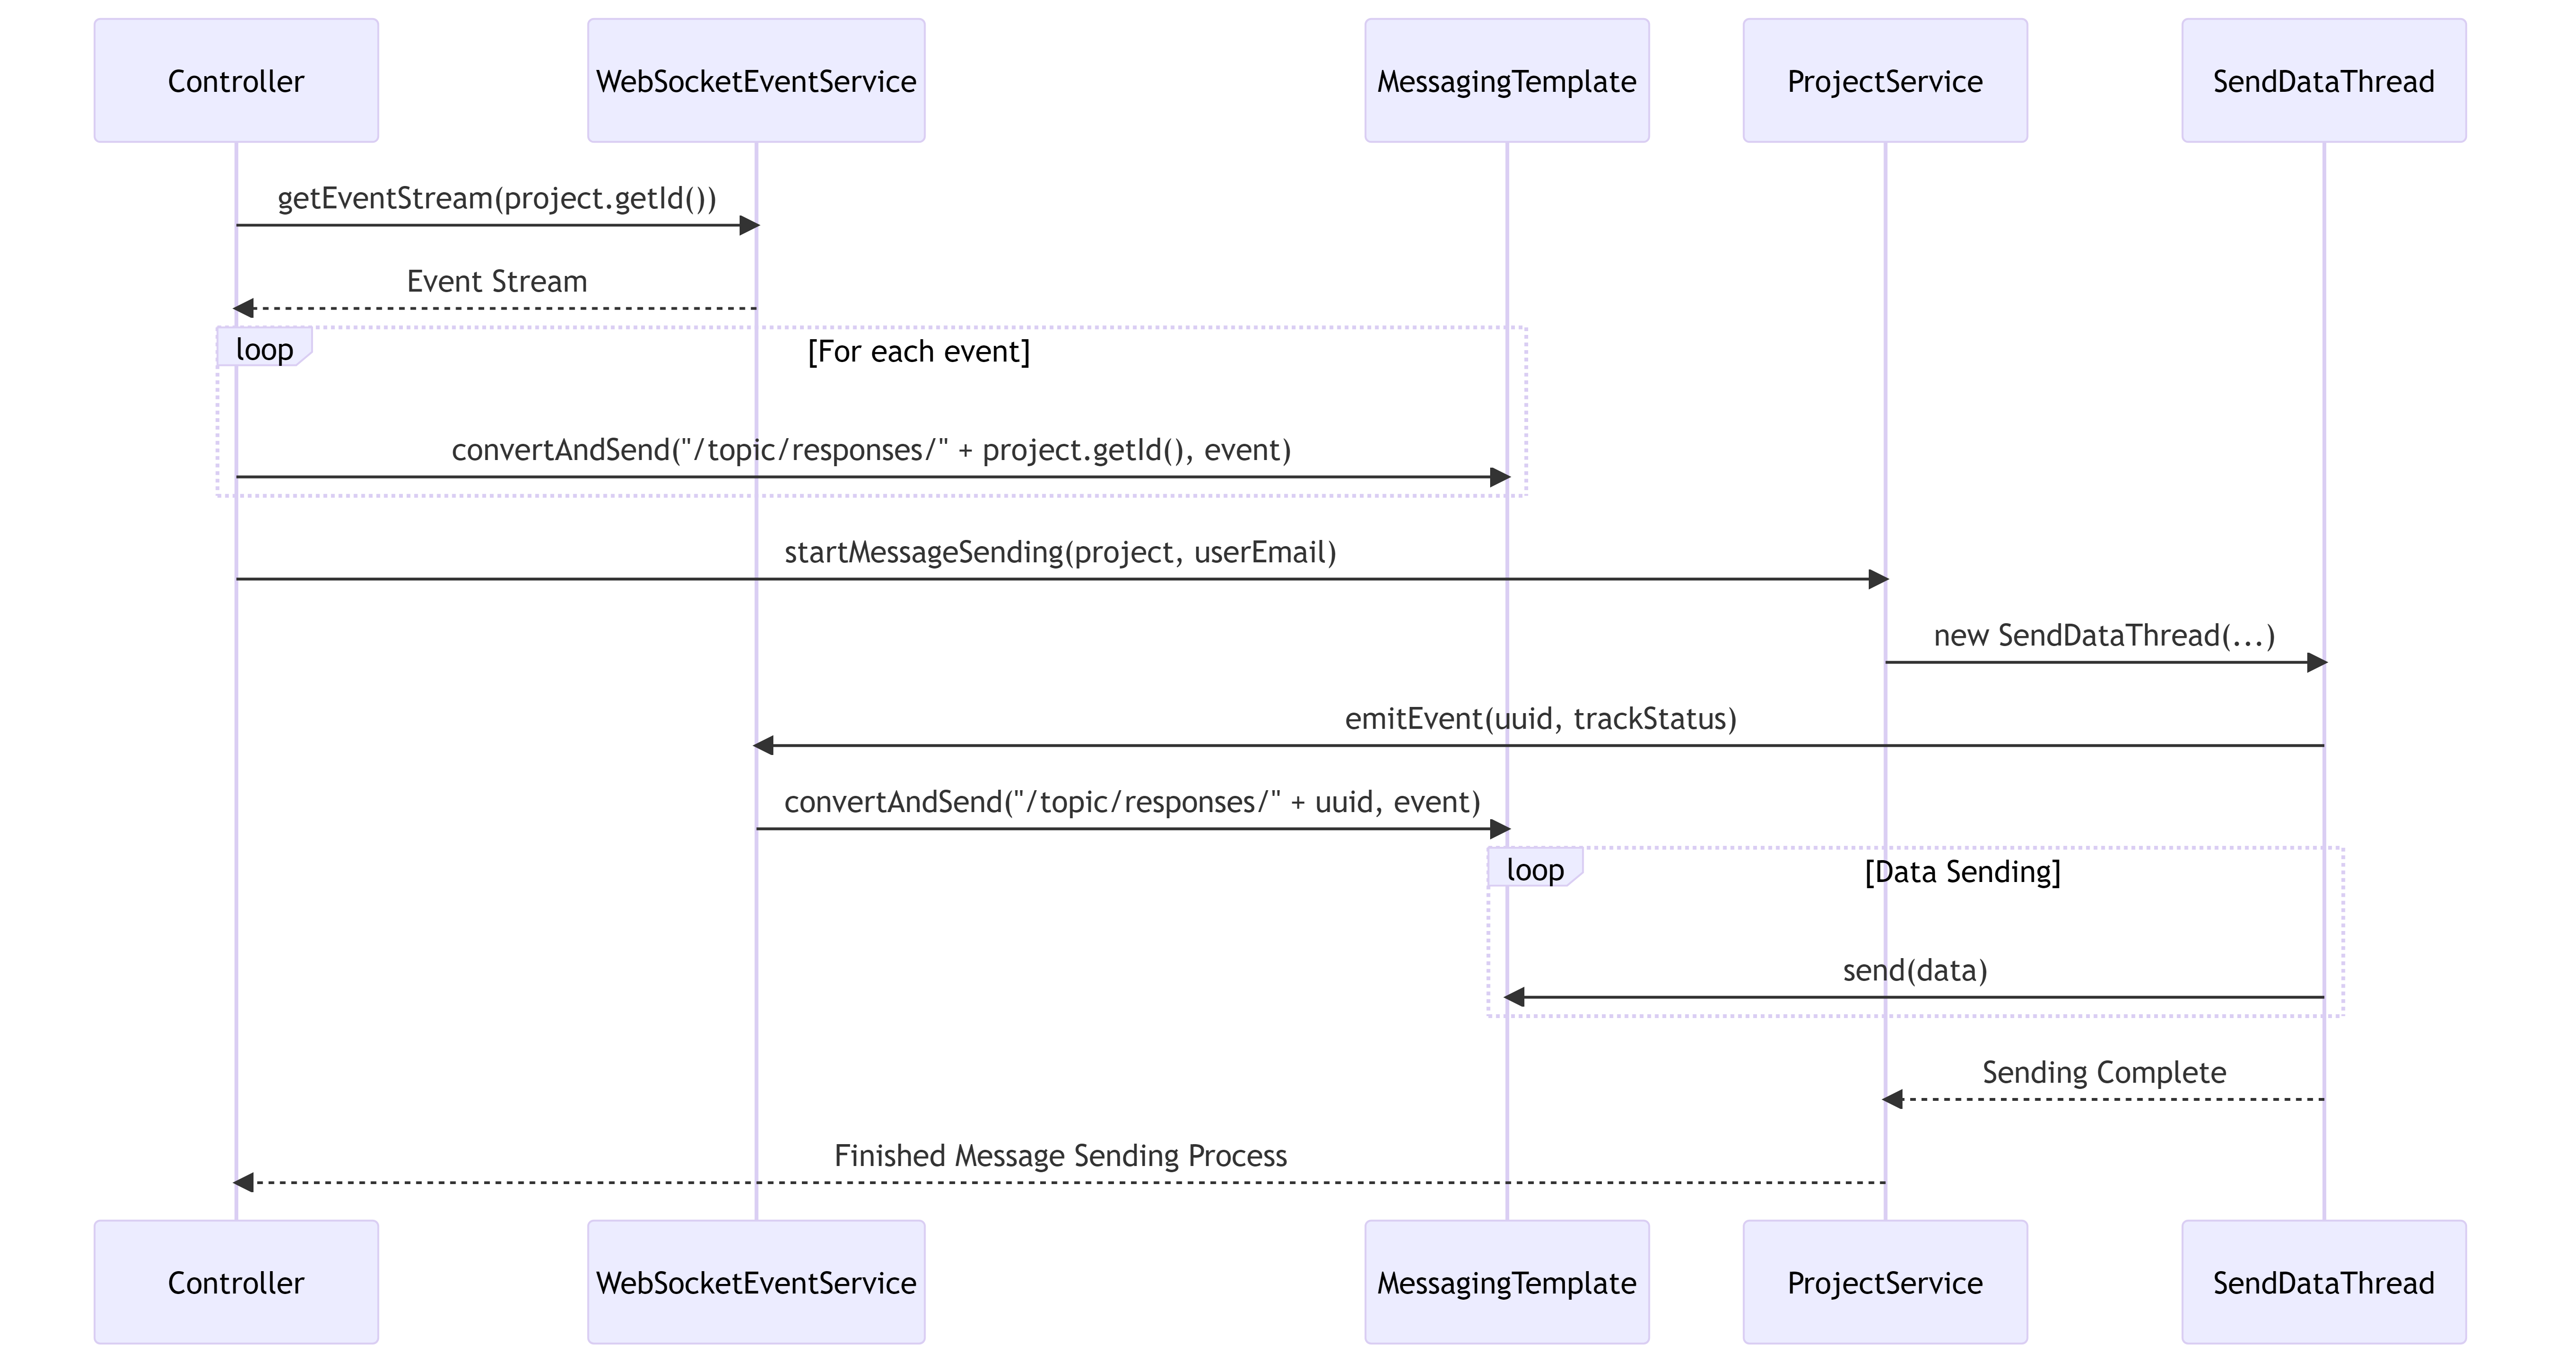
\includegraphics[width=1\linewidth]{includes/figures/EventService.png}
    \caption{vereinfachter Ablauf des Sendens von Statusinformationen mittels eines eigenen EventServices}
\label{fig:java_event_service}
\end{figure}

Hierzu wurde ein eigener EventService eingerichtet, welcher über den aktuellen Fortschritt von allen Threads informatiert wird.
Wie in Figur \ref{fig:java_event_service} zu sehen ist, informieren die einzelnen Threads den EventService über einen wechsel des sendenden DataSets innerhalb eines Tracks.





\subsection{Kommunikation mit der Django API über REST-Clients}
\label{sec:javaRestClient}
Microservices zeichnen sich dadurch aus, dass sie unabhängig voneinander agieren und arbeiten können. Die Kommunikation ziwschen den Services erfolgt über RESTCalls.
Da in der aktuellen Architecktur nur der Spring Service Daten vom Django Service nutzt, muss in Spring hierzu einen RESTClient implementieren, welcher die Anfragen an den anderen Service sendet und die Antworten verarbeitet.

Die Kommunikation zwischen den Services wird über JSON geregelt, wodurch die Kommunikation unabhängig von der Programmiersprache ist.

Anfänglich wurde hierfür die Webflux API von Spring verwendet, da die reine WebClient API nicht ausreichend war und den Implementationsaufwand unnötig erhöht hätte.
Mit der Version 3.2.0 von Spring boot wurde eine neue WebClient API eingeführt, welche Funktional ähnlich der in Quarkus genutzten RestClient API\footnote{https://quarkus.io/guides/rest-client-reactive} ist und daher die Nutzung erleichtert (durch Reduktion des Boilderplate Codes) und das automatische Entitätsmapping übernimmt, wurde die Webflux API durch die neue WebClient API ersetzt.

Der WebClient kommt auch mit einer Failsafe API, auf die aber verzichtet wurde.
Fehlercodes werden durchgereicht, aber erneutes senden von Requests wird nicht durchgeführt. Sollte die DjangoAPI nicht erreichbar sein, wird nur der Fehler an den Nutzer weitergegeben. 
Erneutes senden von Requests würde, sofern die Django API noch existiert, diese nur weiter belasten und der Nutzer wäre von enormen Delays betroffen, welche seine Konfiguration unvorhersehbar machen würden. Dies ist Kontraproduktiv.
Unvollständige DataSets zu senden ist auch keine valide Strategie, da dies im zu testenden System zu ungewollten Verhalten führen würde.

% !TeX program = xelatex

\section{Django}
Pyhton bietet 4 große Webframeworks an. Django, Flask, FastAPI und Pyramid. 
Django ist das bekannteste und am weitesten verbreitete Framework. Es ist ein Full-Stack-Framework, 
das viele Funktionen und Bibliotheken mitbringt, um die Entwicklung zu vereinfachen. Flask ist ein Microframework, das nur die grundlegenden Funktionen bietet, ansonsten eigenständig erweitert werden muss.
Pyramid ist ein Framework, das sich in der Mitte dieser beiden Frameworks befindet. Es bietet mehr Funktionen als Flask, ist aber nicht so umfangreich wie Django. 
FastAPI hingegen ist ein neues Framework, welches auf Geschwindigkeit ausgelegt ist. Es ist noch ein recht neues Framework, welches noch in der Entwicklung steckt und daher nicht die Stabilität oder den Umfang anderer besitzt.
Um eine stabile, wartbare und erweiterbare Software zu entwickeln, wurde daher Django als Framework ausgewählt.

\subsection{Django API Architektur}
Die Spring-Boot-Architektur ist von Regeln und Design Patterns geprägt, um flexibel und möglichst generisch agieren zu können. 
Unterstützt durch die objektorientierte Architektur von Java und Spring Injections, ist dies notwendig.

Python hingegen ist keine rein objektorientierte Sprache, sondern eine Skriptsprache, die OOP-Ansätze unterstützt, diese aber nicht erzwingt. 
Eine klare Trennung in Schichten ist hier nicht so einfach und würde oft zu erhöhtem Aufwand und unnötigem Boilerplate-Code führen. In Django werden Aufgaben in eigene Apps unterteilt, 
wobei sich die Aufgaben der Django API grob in drei Bereiche aufspalten lassen. Die Basis für beide Ansätze sind Daten, daher findet der Upload und die Vorverarbeitung von Daten in einer 
"shared" App statt. Dort sind auch die später detaillierter erklärten Imputationsalgorithmen und die Datenvorverarbeitungslogik angesiedelt.

Machine Learning und Time Series Analysis verhalten sich grundsätzlich unterschiedlich und erhalten daher jeweils ihre eigene App, was auch mit verschiedenen URL-Pfaden einhergeht und die Funktionalitäten logisch voneinander trennt.

Innerhalb der Apps wird die Architektur festgelegt. Da Interfaces und Dependency Injection nicht direkt Teil von Django sind und nur über zusätzliche Pakete und Frameworks eingebunden werden können, 
was zusätzliche Komplexität bedeutet, wurde hierauf verzichtet und eine dreischichtige Architektur gewählt. Diese unterteilt sich in Views, Services und Datenbankaktionen. Views sind fachlich äquivalent zu 
Spring-Controllern und definieren daher die REST-Endpunkte, deren Pfade zentral in einem separaten "urls.py" festgelegt werden. Die Services, hauptsächlich für CRUD-Funktionalitäten genutzt, bilden das Logik-Layer ab. 
Sie sind nicht für das Trainieren der ML-Modelle zuständig, da dies über Websockets gesteuert wird, welche separat definiert werden. Im TSA-Bereich kümmert sich ein Endpunkt um die Datenerstellung, 
da diese fast sofort zugänglich sind und kein Websocket benötigt wird.

Um die Logik der Algorithmen von der CRUD-Funktionalität zu trennen, wurden diese in separate Ordner und Strukturen eingebunden. Die Software muss flexibel sein und eine einfache Integration neuer 
Algorithmen ermöglichen. Ein Builder Pattern, das sich einfach erweitern lässt und die Komplexität des Aufbaus eines komplexen Objekts reduziert, bietet sich hierfür an. Es ist durch den Einsatz von 
Default-Implementierungen einfach einsetzbar, ohne neu konfiguriert werden zu müssen. Dieses Konzept funktioniert jedoch nicht im Bereich der verschiedenen Algorithmen. Hier ist es notwendig, sich auf eine 
Basisklasse zu stützen, die gemäß dem OOP-Prinzip bestimmte Funktionalitäten bereitstellt. Alle neuen Algorithmen müssen von dieser Klasse erben und die erforderlichen Funktionen überschreiben oder nutzen.

Im Datenbankdesign existieren die Algorithmen, und ein Strategy Pattern liefert basierend auf der gegebenen Konfiguration den passenden Algorithmus zurück.


\begin{figure}[htbp]
    \centering
\begin{forest}
    for tree={
    font=\ttfamily,
    grow'=0,
    child anchor=west,
    parent anchor=south,
    anchor=west,
    calign=first,
    edge path={
            \noexpand\path [draw, \forestoption{edge}]
            (!u.south west) +(7.5pt,0) |- node[fill,inner sep=1.25pt] {} (.child anchor)\forestoption{edge label};
        },
    before typesetting nodes={
            if n=1
                {insert before={[,phantom]}}
                {}
        },
    fit=band,
    before computing xy={l=15pt},
    }
    [project
        [djangoproject
                [common]
                [settings.py]
                [urls.py]
        ]
        [mlAPI
                [urls.py]
                [mlalgorithms]
                [services]
                [views]
        ]
        [shared 
            [...]
        ]
        [tsaAPI]
    ]
\end{forest}
\caption{Django Projekt Aufbau}
\end{figure}


\subsection{Absicherung der Anwendung über Djangos Sicherheitskonzept}
Wie bereits in Sektion \ref{sec:javaSpringSecurityConfig} beschrieben, wurde für das Projekt eine JWT-Authentifizierung ausgewählt, um einerseits Nutzer zu verifizieren und andererseits die Daten an Nutzerkonten zu binden.
%TODO: Eine bessere Einleitung könnte noch ergänzt werden.

Django bietet hierfür eine Django-JWT-Library an, die nach einem Spring-ähnlichen Konzept funktioniert, indem eine Middleware eingesetzt wird, die die Validierung gleich zu Beginn durchführt. Hierbei traten jedoch zwei Probleme auf. 
Sowohl Spring als auch Django basieren ihre Authentifizierung auf einem Nutzer-Modell. Die Struktur des Django-Nutzermodells ist allerdings nicht direkt kompatibel mit dem, was Spring verwendet. 
Beide Modelle haben unterschiedliche Felder und sind somit nicht direkt miteinander kompatibel.

Es gibt zwei mögliche Lösungen: Einerseits könnte man auf die normalen Nutzermodelle beider Frameworks setzen. Hierbei müssten weder die Modelle angepasst werden noch die Login- bzw. Passwortvalidierung überschrieben werden. 
Zudem wären beide APIs stärker separiert und somit weniger voneinander abhängig. Nachteilig wäre allerdings die doppelte Nutzerverwaltung und der doppelte Anmeldeprozess. Obwohl dieser durch das Frontend abstrahiert werden könnte, 
bleibt die Lösung suboptimal. Eine Option wie OAuth2 wurde ebenfalls verworfen, sodass nur die Anpassung der Modelle als Lösung verbleibt.

Dabei traten einige Probleme auf. Spring und Django unterscheiden sich in der Art und Weise der Nutzer- und Passwortvalidierung und setzen auf unterschiedliche Verschlüsselungsalgorithmen. Da die Priorität der Spring-API höher ist und die Django-API lediglich die Funktionalität der Spring-API erweitert, muss sich die Django-API nach den Vorgaben von Spring richten.

Um Nutzer in Django ähnlich wie in Spring an Methoden binden zu können, wurde ein ähnliches Modell verwendet. Python besitzt zwar kein direktes AOP-Modell, verfügt jedoch über ein ähnliches Interceptor-System.

\begin{lstlisting}[language=Python, caption={Annotation basiertes Anbinden eines Nutzermodelles an eine Methode}, label={code:djangoSecurity}]
def jwt_authenticated(view_func):
    @wraps(view_func)
    def _wrapped_view(request, *args, **kwargs):
        if not request.user.is_authenticated:
            return Response({'detail': 'Authentication credentials were not provided.'},
                            status=status.HTTP_403_FORBIDDEN)
        return view_func(request, request.user, *args, **kwargs)

    return _wrapped_view
\end{lstlisting}

Wie in Listing \ref{code:djangoSecurity} ersichtlich, fängt dieser Interceptor den Methodenaufruf ab und prüft, ob der Nutzer authentifiziert ist. Ist dies nicht der Fall, wird der Request abgewiesen. Andernfalls wird der Nutzer als Argument an die 
Methode angehängt und ist somit im Code verwendbar.

Dieses Modell ist nicht ideal, da der Nutzer bereits am Controller (oder View) angebunden ist und durch die verschiedenen Schichten weitergereicht werden muss. Daher kann er nicht einfach ersetzt oder ausgetauscht werden, ohne signifikante Teile des Codes 
zu verändern. Eine Alternative wäre die Nutzung eines thread-local Stores, um den Nutzer wieder in den DatenbankService zu verlagern und somit vom Business-Code zu trennen, wodurch er einfacher veränderbar wäre. Dieser Ansatz wurde zwar ausprobiert, 
erwies sich jedoch nicht als stabil genug und wurde letztendlich verworfen.

Im Django-Datenmodell hängen nicht alle Elemente an einem zentralen Punkt, wie es beispielsweise in der Spring-API der Fall ist. Hier ist der Nutzer nur an bestimmten Entitäten angebunden. Die grundlegenden Modelle im Bereich Machine Learning oder 
Time Series Analysis sind unabhängig vom Nutzer und stehen jedem zur Verfügung. Die hochgeladenen Daten und die Konfigurationen, die aus den Daten erstellt werden und später auch in Spring genutzt werden sollen, sind jedoch stark nutzerabhängig und sollten 
dementsprechend auch nur von ihm abrufbar sein.


\subsection{Bidirektionale Kommunikation über Django Channels}
Maschinelles Lernen ist ein sehr rechen- und zeitintensiver Prozess, der im klassischen Call-Response-Prinzip von \ac{REST} schlecht aufgehoben ist. Nutzer reagieren, besonders im \ac{UI}-Umfeld, sehr sensibel auf 
Verzögerungen und fehlendes visuelles Feedback. Es ist wichtig, dass Nutzer sehen können, dass etwas passiert, und sie sollten daher auch über den aktuellen Fortschritt informiert werden.

Die sinnvollste Lösung für dieses Problem ist die Nutzung eines Websockets, der an die Callbacks der Modelle gebunden wird und somit den Nutzer über den aktuellen Fortschritt informiert. 
Django unterstützt Websockets\footcite{https://channels.readthedocs.io/en/latest/} nicht direkt, weshalb hier auf das Framework Channels zurückgegriffen wurde. Channels integriert Websockets 
in Django und bietet somit die Möglichkeit, diese zu nutzen. Channels basiert auf Redis und verwendet es als Message Broker. Redis, wie bereits in \ref{sec:redis} erwähnt, ist eine In-Memory-Datenbank, 
die aufgrund ihrer Schnelligkeit gut für die Kommunikation zwischen Threads geeignet ist.


\begin{lstlisting}[language=Python, caption={Websocket Konsumer}, label={code:djangoWebsocket}]
    class StatusConsumer(JsonWebsocketConsumer):
    runners = {}

    def connect(self):
        group_name = f"model{self.scope['ml_id']}solution{self.scope['sol_id']}"
        try:
            async_to_sync(self.channel_layer.group_add)(group_name, self.channel_name)
            self.scope["group"] = group_name
            self.accept()
        except Exception as e:
            logging.error(e)
            raise UnknownErrorException("cannot connect", reason=str(e))

    def disconnect(self, close_code):
        async_to_sync(self.channel_layer.group_discard)
            (self.scope["group"], self.channel_name)

    def receive_json(self, message, **kwargs):
        response = self.prepare_data(message)
        self.send_json(response)

    def chat_message(self, event):
        self.send_json(event["message"])

    def chat_disconnect(self, event):
        self.send_json(event["message"])
        self.close()
        self.runners.get(event["uuid"])
\end{lstlisting}

Der Code in Listing \ref{code:djangoWebsocket} präsentiert einen JSON-Konsumer, der eine WebSocket-Anfrage annimmt und eine Verbindung aufbaut. Aus der initialen 
Anfrage werden die trainingsrelevanten Informationen extrahiert und an die entsprechende Stelle im Prozess weitergeleitet.

Nachdem die Modelle trainiert worden sind, wird der finale Status an den Nutzer gesendet und anschließend die Verbindung getrennt.

\subsection{Fehlerbehandlung und Verarbeitung}
Das System implementiert ebenfalls ein interceptor-basiertes Error-Handling nach dem "Fail-Fast"-Prinzip. Illegale Optionen, invalide Parameter und ungültige Dateitypen führen zum Auslösen einer 
Exception, die von speziell dafür vorgesehenen Exception-Handlern abgefangen und verarbeitet wird. Auch hier wurde ein Format gewählt, das der Spring-Variante ähnelt, um ein kohärentes und einheitliches 
Fehlermeldungsprinzip zu gewährleisten.

\begin{lstlisting}[language=Python, caption={Exception Handler}, label={code:djangExceptionHandler}]
def exception_handler(exc, context):
    def build_error_response(exception, status_code):
        response_data = {
            "error": str(exception),
            "reason": exception.reason if hasattr(exception, 'reason') else None,
            "i18nKey": exception.i18nKey if hasattr(exception, 'i18nKey') else "UNDEFINED"
        }
        return JsonResponse(response_data, status=status_code)

    exception_mapping = {
        NotFoundException: status.HTTP_404_NOT_FOUND,
        BadRequestException: status.HTTP_400_BAD_REQUEST,
        InvalidFileTypeException: status.HTTP_400_BAD_REQUEST,
        UnknownErrorException: status.HTTP_500_INTERNAL_SERVER_ERROR,
        UniqueConstraintViolationException: status.HTTP_409_CONFLICT,
        UserNotAuthenticated: status.HTTP_403_FORBIDDEN
    }

    if type(exc) in exception_mapping:
        return build_error_response(exc, exception_mapping[type(exc)])

    if isinstance(exc, UnknownErrorException):
        logging.error(f"unknown error: {exc}")

    response = drf_exception_handler(exc, context)
    if response is not None:
        return response

    return JsonResponse({'error': 'Unexpected server error'}, 
        status=status.HTTP_500_INTERNAL_SERVER_ERROR)
\end{lstlisting}

Die in Listing \ref{code:djangExceptionHandler} dargestellte Exception Map ermöglicht es, selbst definierte Exceptions auf einen \ac{REST} Error Code zu projizieren. Dadurch ist sie flexibel in der Nutzung und leicht anpassbar.


\subsection{Validierung der Daten und Vorverarbeitung}
\label{sec:djangoDataPreprocessing}
Es ist nicht davon auszugehen, dass alle Daten in einer homogenen Form vorliegen und normalisiert sind. Dies stellt jedoch eine grundlegende Anforderung dar, nicht nur um die Modelle effektiv konstruieren zu können, sondern auch um ...

\paragraph*{Fehlende Werte im Datensatz}
Die Handhabung von Daten in Zeitreihen stellt eine besondere Herausforderung dar, insbesondere wenn nicht sichergestellt ist, dass die Daten immer im gleichen Abstand aufgezeichnet oder mit Zeitstempeln versehen wurden. Unter diesen Bedingungen wurde ein Algorithmus entwickelt, der die Struktur der Daten erkennt, sie entsprechend kategorisiert oder umwandelt und in ein uniformes Format überführt.

Angesichts der Komplexität, die mit der Unterstützung verschiedener Dateiformate einhergeht, wurden einige Annahmen getroffen:
\begin{enumerate}
    \item Bei mehreren unbenannten Datensätzen in einer Datei wird geprüft, ob eine dieser Zeitreihen konsequent linear ansteigt. Ist dies der Fall, werden diese Werte als Zeitstempel interpretiert.
    \item Ist keine konsequent steigende Zeitreihe zu finden, wird den Daten ein normaler Anstieg zugeordnet.
    \item Dateiformate wie JSON oder CSV, die Header oder Dictionaries nutzen, erfordern eine spezielle Taxonomie, um die Zeitreihe im Dokument zu identifizieren, die für die Zeiterfassung gedacht ist. Wenn eine solche gefunden wird, wird sie jeder Zeitreihe hinzugefügt.
\end{enumerate}

Basierend auf diesen Annahmen wurde ein Algorithmus entwickelt, abhängig vom Datenformat. Dieser durchsucht die Datei, testet auf mögliche Strukturen und bearbeitet sie anschließend, wie in Abbildung \ref{fig:upload_data} dargestellt.

\begin{figure}[h]
    \centering
    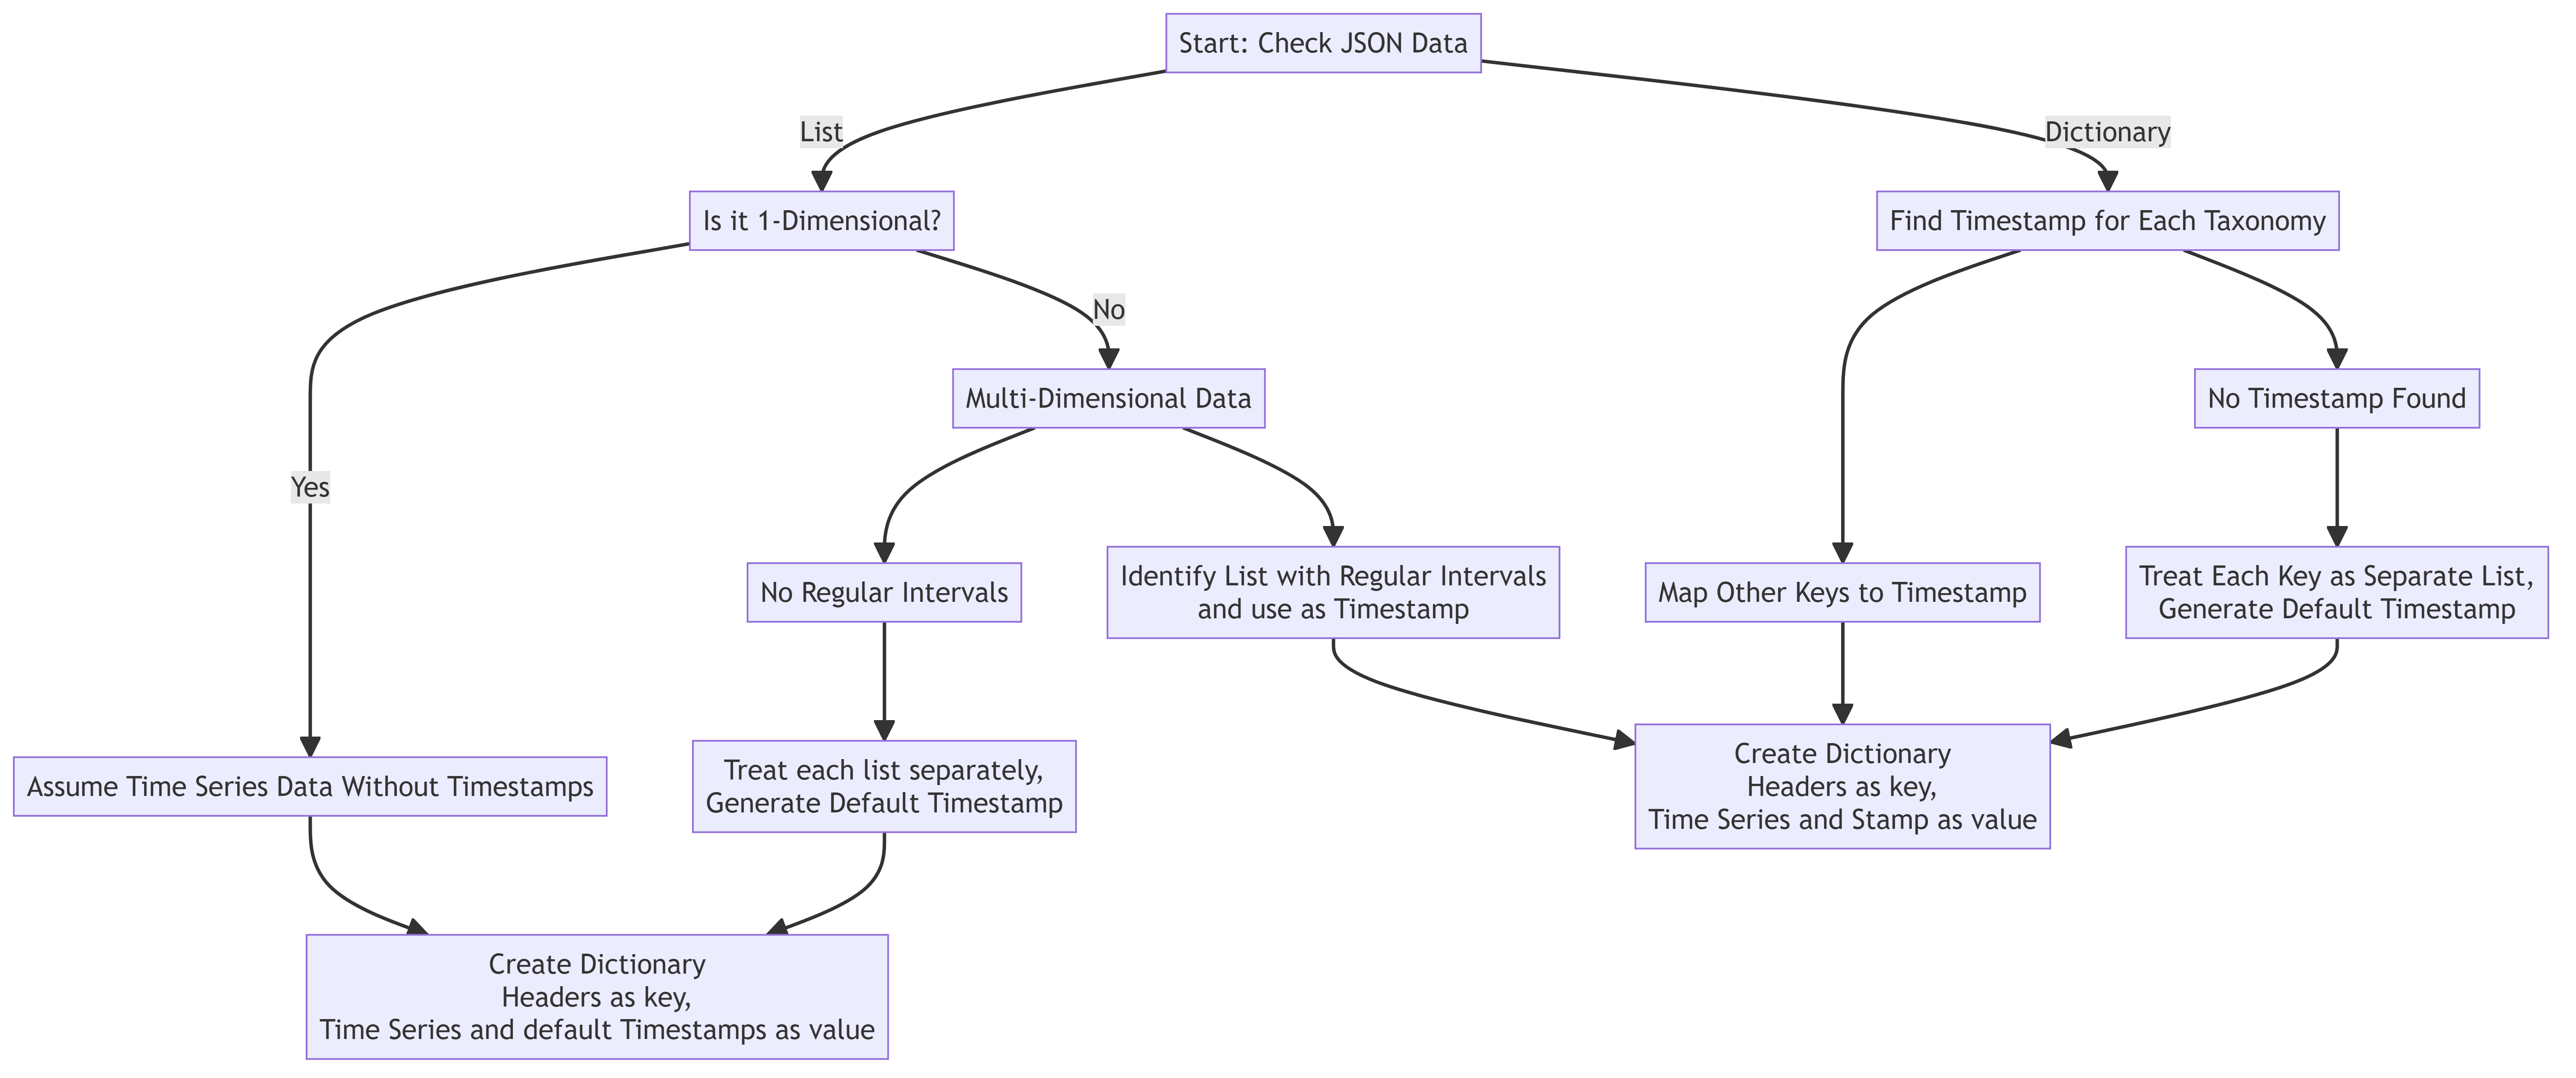
\includegraphics[width=0.9\linewidth]{includes/figures/upload_process.png}
    \caption{Algorithmus zum zerlegen einer hochgeladenen JSON Datei}
\label{fig:upload_data}
\end{figure}



Diese Vorverarbeitung der Daten erfolgt bereits beim Hochladen und stellt sicher, dass die Daten im weiteren Verlauf immer in einem uniformen Format vorliegen. 
Die Überprüfung der Daten auf Lücken wird erst bei Bedarf durchgeführt. Da nur die Zeitstempel eine Rolle spielen und diese im Unix-Format vorliegen, berechnet der Algorithmus die Differenz aufeinanderfolgender Werte. Hierbei wird ein Schwellenwert definiert, um kleine Ungenauigkeiten zu ignorieren. Bei signifikanten Abweichungen von der Standarddistanz wird eine Lücke angenommen.

Der Algorithmus zum Identifizieren und Füllen von Lücken ist in Listing \ref{enum:django_gap_handling} zu finden. Er beschreibt, wie Lücken nach bestimmten Kriterien 

definiert werden und zeigt auf, wie diese geschlossen werden. In diesem Schritt werden die Lücken noch nicht klassifiziert oder gefüllt, sondern lediglich mit \textit{NaN}-Werten markiert. Dadurch entsteht eine Zeitreihe, in der alle Werte in regelmäßigen Abständen vorhanden sind.

\begin{lstlisting}[language=Python, caption={Algorithmus zum Auffüllen von Lücken}, label={code:djangoAlgoGap}]
def __find_differences_in_steps_and_fill_them_with_nan(train_data, timestamps_normalized):
    processed_train_data = []
    processed_time_stamps = []
    for i, (train_d, timestamp_d) in enumerate(zip(train_data, timestamps_normalized)):
        differences = np.diff(timestamp_d)
        threshold = differences.min() + differences.min() * error_percentage
        large_gap_indices = np.where(differences > threshold)[0]
        start_gap = large_gap_indices
        end_gap = large_gap_indices + 1
        diff = np.ceil(-(differences[end_gap] - differences[start_gap]) / threshold)
        new_timestamps = np.copy(timestamp_d)
        new_train_d = np.copy(train_d)
        for index, size in sorted(zip(end_gap, diff), key=lambda x: x[0], reverse=True):
            nan_array = np.full(int(np.round(size)), np.nan)
            new_timestamps = np.insert(new_timestamps, index, nan_array)
            new_train_d = np.insert(new_train_d, index, nan_array)
        processed_train_data.append(new_train_d)
        processed_time_stamps.append(new_timestamps)
    return processed_train_data, processed_time_stamps
\end{lstlisting}

Für das Füllen von Lücken wurden unterschiedliche Ansätze abhängig von der Größe der Lücke gewählt. Kleine Lücken werden durch Imputationsalgorithmen gefüllt, indem die umgebenden Werte herangezogen werden, um die wahrscheinlichsten Ersatzwerte zu ermitteln. 
Es wurden verschiedene Algorithmen implementiert, zwischen denen der Nutzer per Eingabe im Frontend wählen kann. Diese Algorithmen werden als Funktion übergeben, erhalten die relevanten Daten und liefern die aufgefüllte Version zurück. Dies ermöglicht ein sehr 
flexibles Vorgehen und kann daher auch ohne großen Aufwand erweitert werden. Bei größeren Lücken, wo der Informationsverlust zu groß wäre, bleiben die Werte leer und erhalten den in Python üblichen \textit{NaN}-Wert (Not a number). Die Handhabung dieser leeren Werte obliegt den nachfolgenden Algorithmen, die in den Sektionen \ref{sec:djangoML} und \ref{sec:djangoTSA} näher erläutert werden.

\paragraph{Uniformisierung der Daten}
Eine uniforme Version der Daten ist besonders wichtig im Bereich des maschinellen Lernens, da Trainingsdaten in unterschiedlichen Längen und Bereichen (beispielsweise von 0 bis 1) die Ergebnisse verfälschen oder das Training erschweren können. Daher ist es notwendig, die Daten zu normalisieren und auf eine einheitliche Länge zu bringen. 
Oft ist auch eine Reduzierung oder Komprimierung der Daten sinnvoll. Zwar gehen dabei Informationen verloren, aber da die Grundstruktur des Datensatzes erhalten bleibt und die Performance des Modells 
deutlich erhöht wird, sollte diese Option den Nutzern angeboten werden. Teilweise ist dies auch notwendig, da Modelle ab einer gewissen Größe nicht mehr auf jeder Hardware laufen.

Den Nutzern werden viele Möglichkeiten gegeben, selbstständig die Komprimierung vorzunehmen und eventuell lineare Trends aus den Daten zu entfernen. Weitere Optionen können problemlos hinzugefügt werden, da dafür lediglich ein JSON-Schema, die Implementierung sowie die Integration in das Strategy Pattern notwendig sind. Alle Änderungen im Vorverarbeitungsschritt werden in der Datenbank gespeichert und sind umkehrbar, sodass beim späteren Versenden der Daten diese wieder in der Form vorliegen, in der die Originaldaten hochgeladen wurden. Die verschiedenen Implementierungen werden über ein Strategy Pattern gezielt angesprochen und über JSON-Dictionaries mit ihrer spezifischen Konfiguration geladen.



\subsection{Generalisierung und Nutzung der Machine Learning Modelle}
\label{sec:djangoML}
Python ist eine der führenden Sprachen im Bereich des maschinellen Lernens und bietet daher eine umfangreiche Auswahl an Bibliotheken und Frameworks, die mit hilfreichen Komponenten und Funktionen ausgestattet sind. 
Große Frameworks wie TensorFlow oder PyTorch bieten zahlreiche Möglichkeiten, sind jedoch auch sehr komplex und erfordern viel Zeit, um gewünschte Modelle zu entwickeln. Aus diesem Grund wurde in diesem Projekt auf Keras gesetzt, 
das eine Abstraktionsebene über TensorFlow bietet und somit die Komplexität reduziert. Keras ermöglicht das Erstellen von Modellen über ein \ac{ANN}, die sich durch die Konfiguration der Schichten und Neuronen anpassen lassen.

Wie im Kapitel \ref{cha:stateOfTheArt} ersichtlich, sind \acp{GAN} und \acp{RNN} verbreitete Ansätze, um aus einer Menge von Trainingsdaten synthetische Daten zu generieren. Da ein Ziel dieser Arbeit der Vergleich dieser Ansätze ist, 
wurden verschiedene Modelle beider Varianten implementiert.

In der Praxis unterscheidet die Django-API nicht zwischen den beiden Varianten, da beide über dasselbe Interface angesprochen werden. Das zugrundeliegende Strategy Pattern liefert die passende Implementierung.


\begin{lstlisting}[language=Python, caption={Grundklasse zum Trainieren der Machine Learning Modelle, sie stellt Grundmethoden und geteilte Funktionalitäten bereit}, label={code:djangoAlgoGAN}]    
class GeneralMLModel:
    data: List[np.ndarray] = None
    run_information: RunInformation = None

    def set_config(self, config: RunInformation):
        """ set configuration for model """
        pass

    def set_data(self, data: List[np.ndarray]):
        """ set data for model """
        pass

    def run(self):
        """ start training the model  """
        pass

    def predict_data_from_model(self):
        """ predict data from model """
        pass

    def forcast(self, limit: int, starting_point: int = -1) -> np.array:
        """ forcast data from model, does not work for every model """
        pass

    def save(self, model: Model) -> RunInformation:
        """ write model to file and save base64 string in database """
        pass

    def load_model(self) -> Model:
        """ write model from database to file and load it from there """
        pass

    def create_image(self, real: List[np.array], synthetic: List[np.array], title: str):
        """ create an image and save it as base64 string """
        pass
\end{lstlisting}

\paragraph{Generative Modelle}
\label{sec:djangoGAN}
Zwei funktionierende \acp{GAN} wurden implementiert: das normale \ac{GAN} und das \ac{CGAN}. Mit \acp{WGAN} und \acp{TGAN} wurde ebenfalls experimentiert, und es existieren Testversionen dieser im Testframework (siehe Abschnitt \ref{sec:tested_models}). 
Da diese jedoch nicht die gewünschten Ergebnisse lieferten, stehen sie momentan nur in der Entwicklungsumgebung zur Verfügung und werden nicht von der API angeboten. Beide implementierten Varianten umfassen einen Generator und einen Diskriminator, 
wobei die Eingabedimensionen von der Länge der zu trainierenden Zeitreihe abhängen. Daher spielt die Normalisierung der Daten eine entscheidende Rolle, um Übereinstimmungen in den Dimensionen der Schichten zu gewährleisten.

\paragraph{Rekursive Modelle}
\acp{RNN} analysieren Daten in ihrer zeitlichen Abfolge und eignen sich daher besonders gut für die Analyse oder Vorhersage von Zeitreihen. Die von ihnen generierten Daten sind stark abhängig von der Variabilität der Trainingsdaten. 
Da sie jedoch in der Lage sind, Vorhersagen über künftige Verläufe zu erstellen, bieten sie Möglichkeiten, die generative Modelle nicht bieten. Deshalb wurden sie in das System integriert. Die Auswahl der Parameter erfolgt allerdings erst in der Spring-API, 
da dort die entsprechenden Datensätze erstellt und die JSON-Schemata mit den dazugehörigen Regeln definiert werden.

\paragraph{Abhängigkeitsprobleme}
Ein wesentliches Problem stellte die Integration weiterer Modelle aus verschiedenen Bibliotheken dar. Viele Bibliotheken befassen sich mit Datengenerierung, sind jedoch untereinander nicht immer kompatibel, was zu Abhängigkeitskonflikten führte. 
Dies verhinderte die direkte Nutzung dieser Bibliotheken.

\subsection{Generalisierung und Nutzung der Zeitreihenanalysealgorithem}
\label{sec:djangoTSA}

Die Zeitreihenanalyse ist der zweite Hauptansatz zur Generierung von Daten. Dabei werden die Daten in ihre Bestandteile zerlegt, um Muster zu erkennen und diese zu nutzen, um neue Daten zu generieren. 
Wie bereits in Kapitel \ref{cha:stateOfTheArt} beschrieben, gibt es verschiedene Ansätze für die Zeitreihenanalyse, die sich in ihrer Komplexität und ihren Ergebnissen unterscheiden.

Zwei vielversprechende Ansätze in diesem Bereich sind die Singular Spectrum Analysis (\ac{SSA}) und die Empirical Mode Decomposition (\ac{EMD}). Diese Methoden zielen darauf ab, Muster in den Daten durch die Zerlegung in 
(\acp{IMF}) zu identifizieren und für die Generierung neuer Daten zu nutzen. Die Implementierung dieser Algorithmen ist zwar rechenintensiv, aber im Vergleich zu maschinellen Lernansätzen nicht so aufwendig, da sie nicht trainiert werden 
müssen und nur einmalig ausgeführt werden. Python bietet bereits Bibliotheken, die diese Algorithmen implementieren. Daher besteht die Herausforderung hauptsächlich darin, die Daten in das richtige Format zu bringen und dem Nutzer Zugriff auf die 
generierten Daten zu gewähren.

Obwohl dieser Ansatz in der Testphase nicht berücksichtigt wurde, bietet die Zerlegung der Daten in ihre Bestandteile einen weiteren interessanten Vorteil für den Nutzer. Da die Daten dem Nutzer grafisch dargestellt werden, 
kann er selbst Muster erkennen und diese nach Belieben verschieben. Dies ermöglicht es ihm, die Ausgangsdaten zu manipulieren und zu verändern, um so neue Daten zu generieren. Der Nutzer behält somit die Kontrolle 
und überlässt sie nicht nur dem Algorithmus. Weitere Details dazu werden im Kapitel \ref{sec:reactTSA} erläutert.

Um weitere Ansätze zu testen und anzubieten, wurden auch klassische Methoden wie die Amplitude Modulation and Noise (AMIRA) und der Cubic Spline Algorithmus implementiert. Diese Methoden interpolieren die Daten und bieten 


somit eine andere Form der Datenabstraktion. Beide Methoden sind sehr schnell und liefern gute Ergebnisse. Allerdings sind sie nicht in der Lage, neue Daten zu generieren, da sie lediglich die vorhandenen Daten interpolieren und nicht nach Mustern suchen.

Die Integration dieser Algorithmen in die API erfolgt ähnlich wie im Kapitel \ref{sec:djangoML} und sie sind ebenfalls über ein Strategiemuster auswählbar.



\subsection{Das Datenbank Modell}

Aus den in den vorherigen Sektionen beschriebenen Anforderungen an die Datenstruktur wurde ein Datenbankmodell entwickelt, das die Anforderungen erfüllt und gleichzeitig flexibel genug ist, um die Erstellung komplexer Simulationsumgebungen zu ermöglichen.
Dieses ist in Abbildung \ref{fig:datamodel_new_version} dargestellt und zeigt den aktuellen Stand der finalen Software.

\begin{figure}[ht]
    \centering
    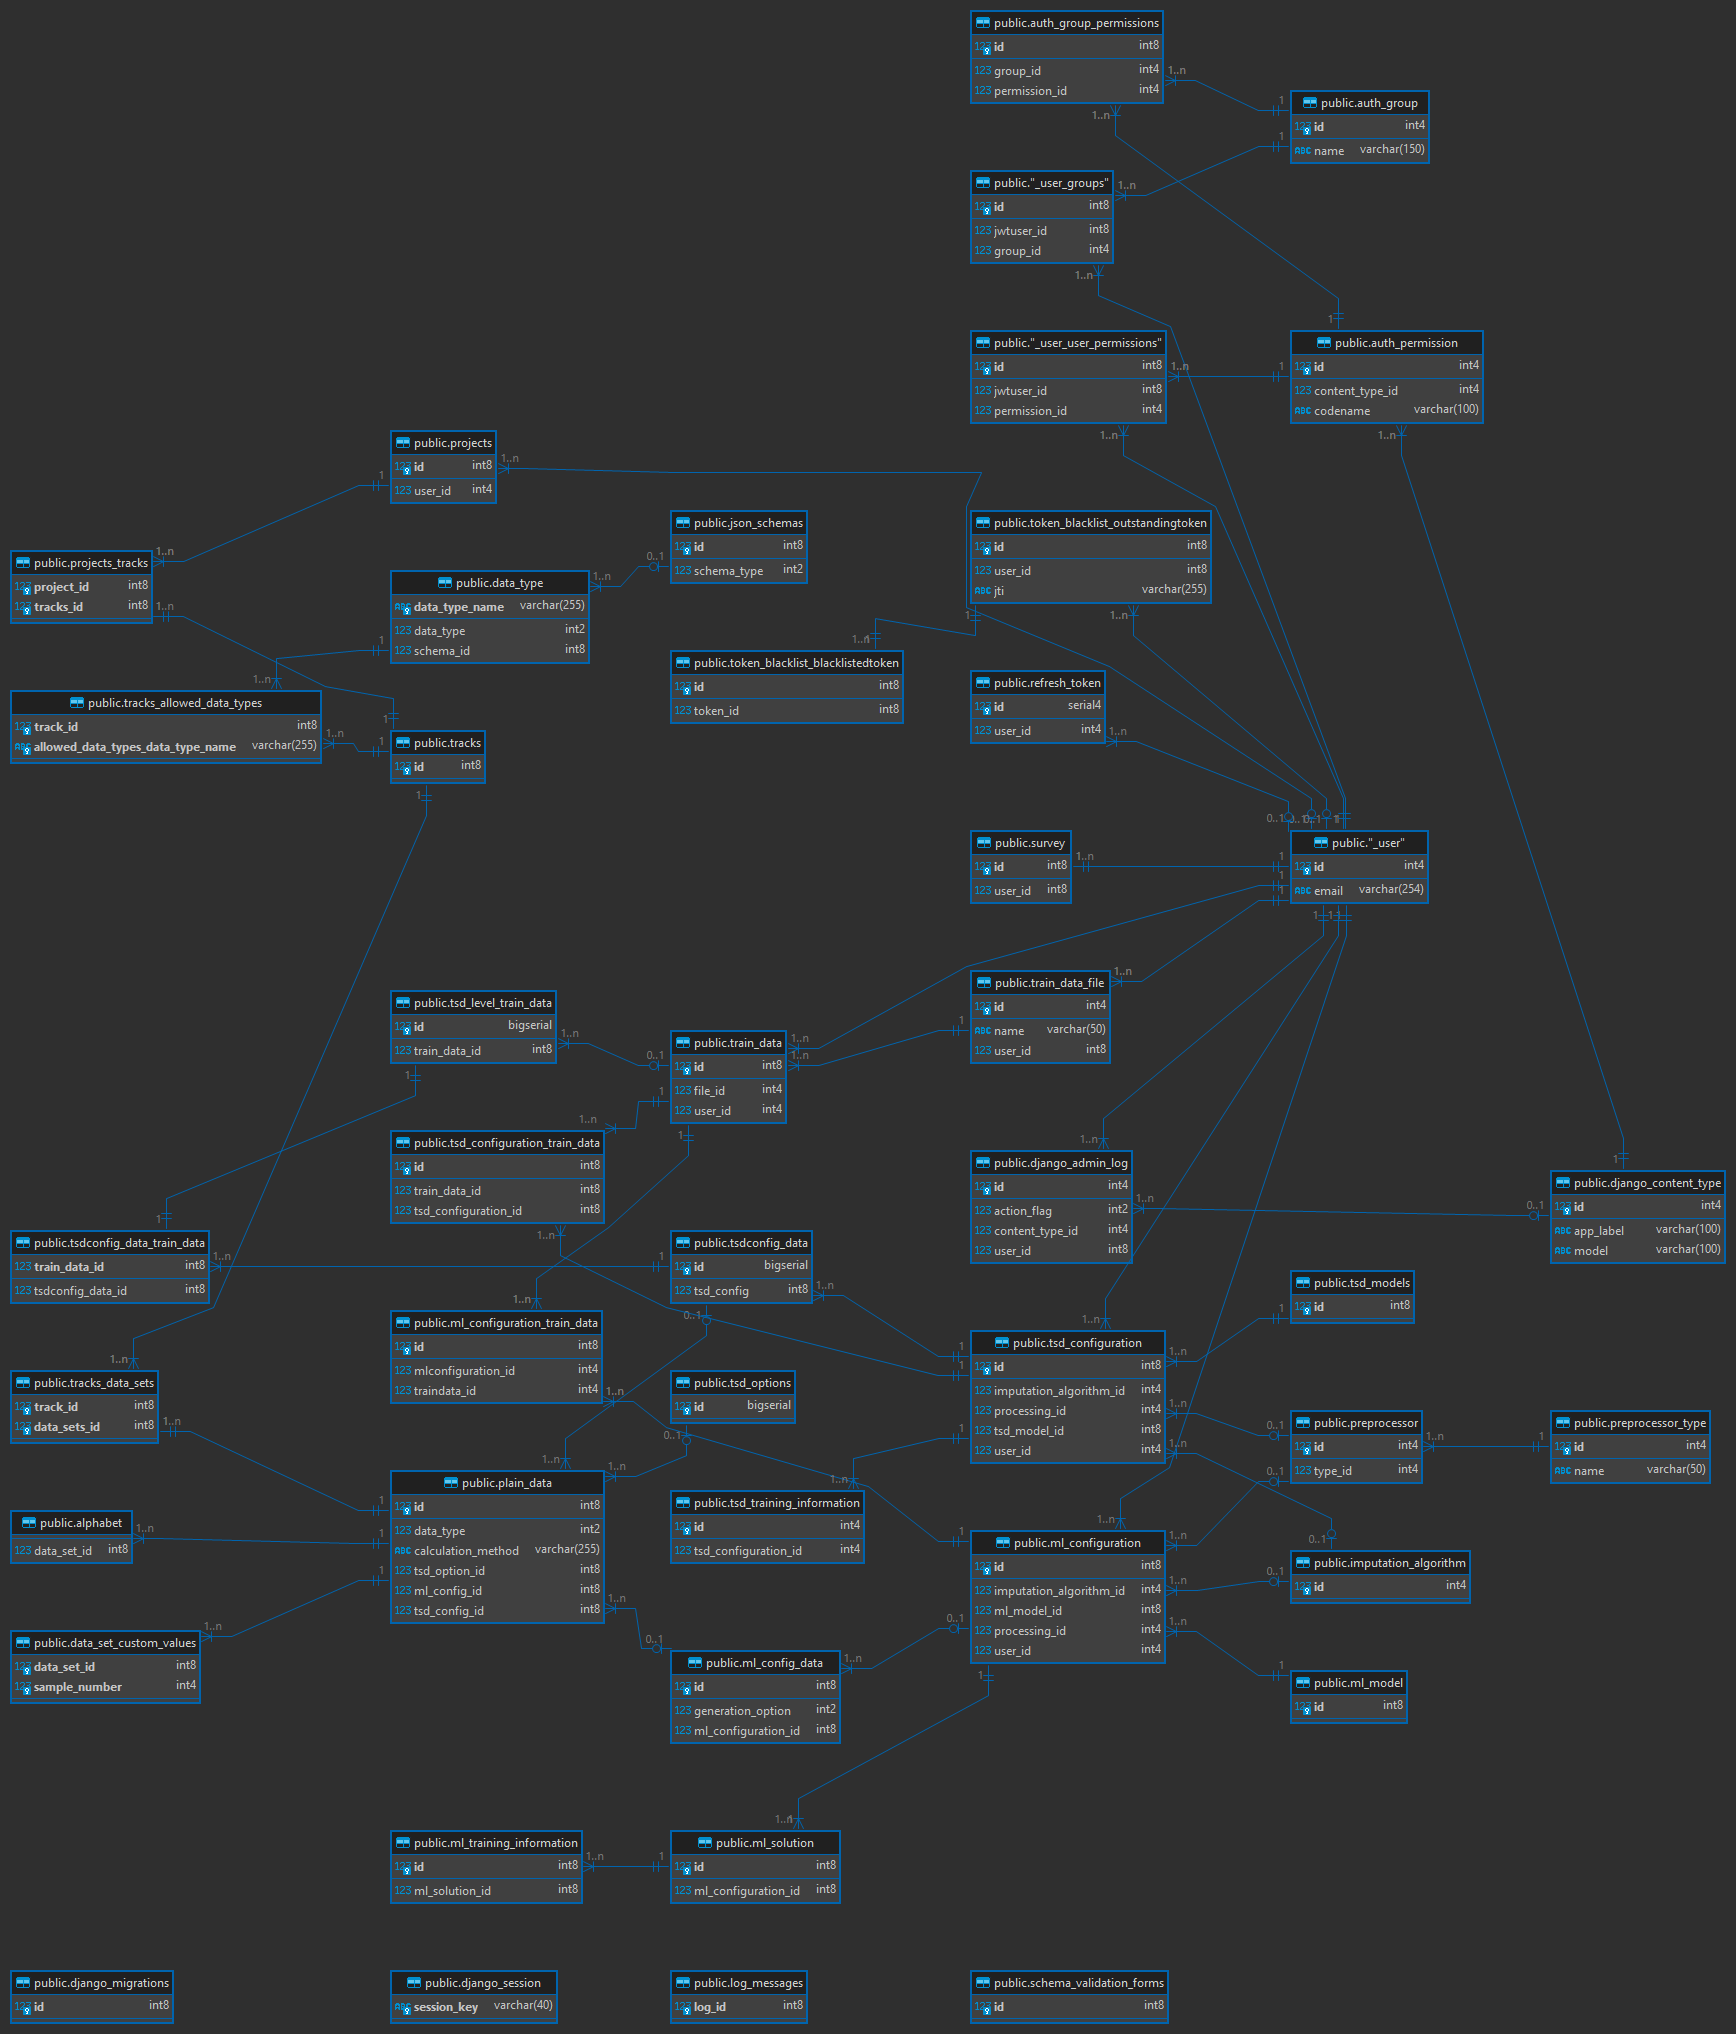
\includegraphics[width=1\textwidth]{includes/figures/database/software.png}
    \caption{Entity-Relationship-Diagramm der aktuellen Datenstruktur}
    \label{fig:datamodel_new_version}
\end{figure}

Wie in dem Bild zu sehen ist, dient der Nutzer als zentraler Punkt und besitzt viele verschiedene Entitäten, die mit ihm verknüpft sind. Wichtig sind hiervorallem die TrainingData, welche die hochgeladenen Daten beinhalten, die Projects, welche seine Projekte aufspannen, und die jeweiligen Konfigurationen für \ac{ML} und \ac{TSA} Modelle.
Die ausenstehenden Entitäten der Schemata sind für die flexibele Zusammensetzung der jeweiligen JSON-Schemata notwendig.

% !TeX program = xelatex
\section{React Implementation}

\subsection{Grundlagen der UI}
\label{sec:reactUI}
Ein zentrales Konzept von React ist die Verwendung von Komponenten. Diese Komponenten sind wiederverwendbare UI-Elemente, die jeweils über eigenes Styling und Verhalten verfügen. 
Der wesentliche Vorteil dieses Ansatzes ist die Förderung von Wiederverwendbarkeit und Konsistenz innerhalb der Applikation. Durch die Wiederverwendung von Komponenten wird eine einheitliche Benutzeroberfläche 
gewährleistet. UI-Elemente verhalten sich in der gesamten Anwendung konsistent. Ein kohärentes Design verbessert die Benutzererfahrung und erfüllt damit zwangsläufig einen der in Sektion \ref{cha:Anforderungsanalyse:Usability} 
vorgestellten Punkte der ISO 9241-110. Zudem fördert dieser Ansatz die Entwicklungseffizienz und hält die Codebasis überschaubar.

\subsection{Grundideen des UI-Designs}
Im Gegensatz zur ursprünglichen Version, die in mehrere Aufgabenbereiche unterteilt war, empfiehlt sich nun die Integration einer zentralen Navigationsleiste für eine bessere Übersichtlichkeit. Diese ermöglicht es den Nutzern, 
problemlos zwischen verschiedenen Bereichen und Menüs zu wechseln, was die Anzahl der Klicks zwischen den Interaktionen reduziert. Dies minimiert nicht nur den Aufwand für den Nutzer, sondern verbessert auch die allgemeine Benutzererfahrung. 
Die im Kapitel \ref{cha:Usability_study} vorgestellte Studie dient zur Überprüfung der hier vorgestellten Konzepte.

Nach dem Login landet der Nutzer auf der Hauptseite, die eine Übersicht über alle verfügbaren Möglichkeiten bietet. Dies umfasst eine kurze Beschreibung des Ablaufs sowie Erklärungen zur Funktionsweise der gewählten Technologien. 
In der Navigationsleiste kann der Nutzer farblich hervorgehoben sehen, wo er sich befindet, und kann zu anderen Bereichen wie der Konfiguration der Modelle, der Verwaltung der Daten oder dem Erstellen von \textit{Projects} navigieren. 
Die Elemente \textit{Studie} und \textit{Dokumentation} sind nur temporär und sollten in der Hauptanwendung entfernt werden. Sie dienen lediglich der Durchführung und Dokumentation der Studie.
\begin{figure}[h]
    \centering
    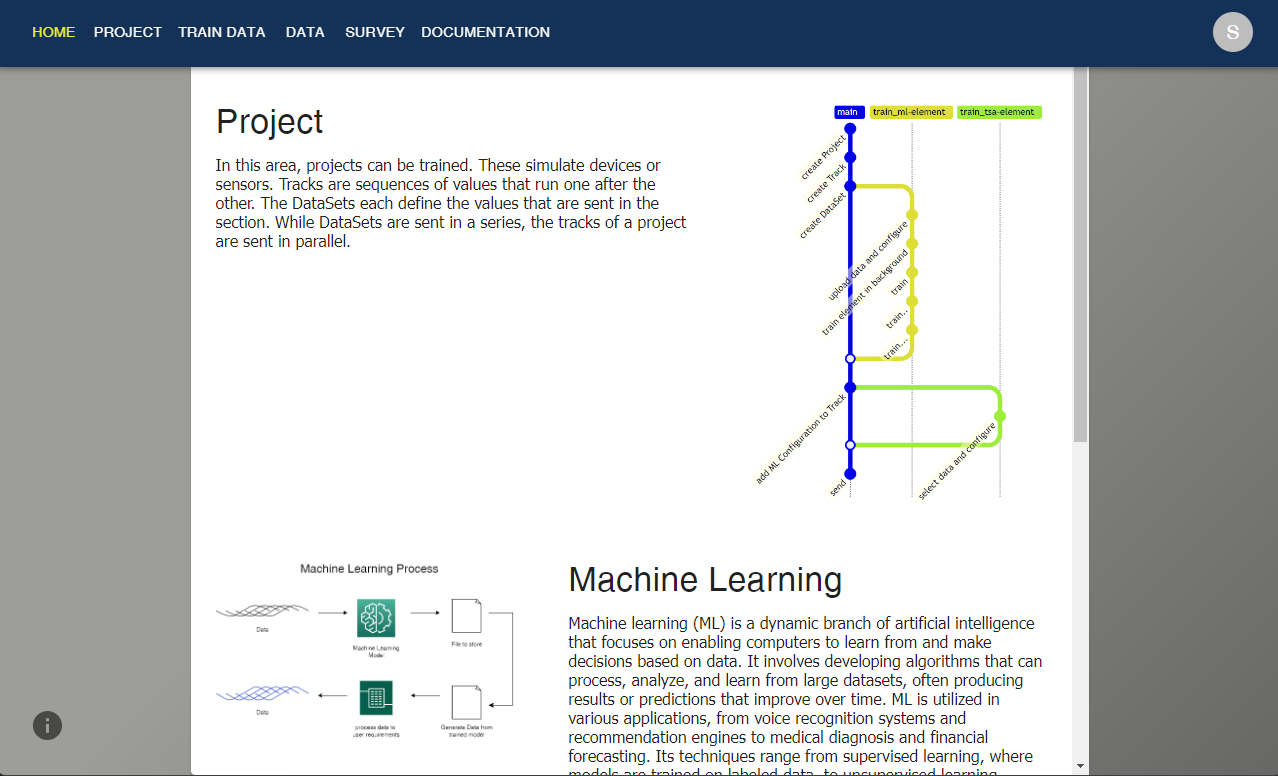
\includegraphics[width=1\linewidth]{includes/figures/new_version/main_page.png}
    \caption{vereinfachter Ablauf des Sendens von Statusinformationen mittels eines eigenen EventServices}
\label{fig:main_page}
\end{figure}





\subsection{Kommunikation mit den APIs}
\label{sec:frontendCommunication}
Um die Kommunikation und Fehlerverarbeitung zwischen den Services zu vereinheitlichen, wurde die Axios-Bibliothek integriert. 
Axios implementiert die Promise-API und ermöglicht somit asynchrones Arbeiten. Es bietet eine automatische Serialisierung von JSON zu TypeScript-Typen und Interfaces, was ein direktes, 
typenbasiertes Arbeiten mit der React-Umgebung erlaubt. Da React zudem Multi-Browser-Unterstützung bietet, kann durch die Auslagerung dieser Problematik auf eine externe Bibliothek die Webanwendung mit allen gängigen Browsern kompatibel gemacht werden.


\begin{figure}[h]
    \centering
    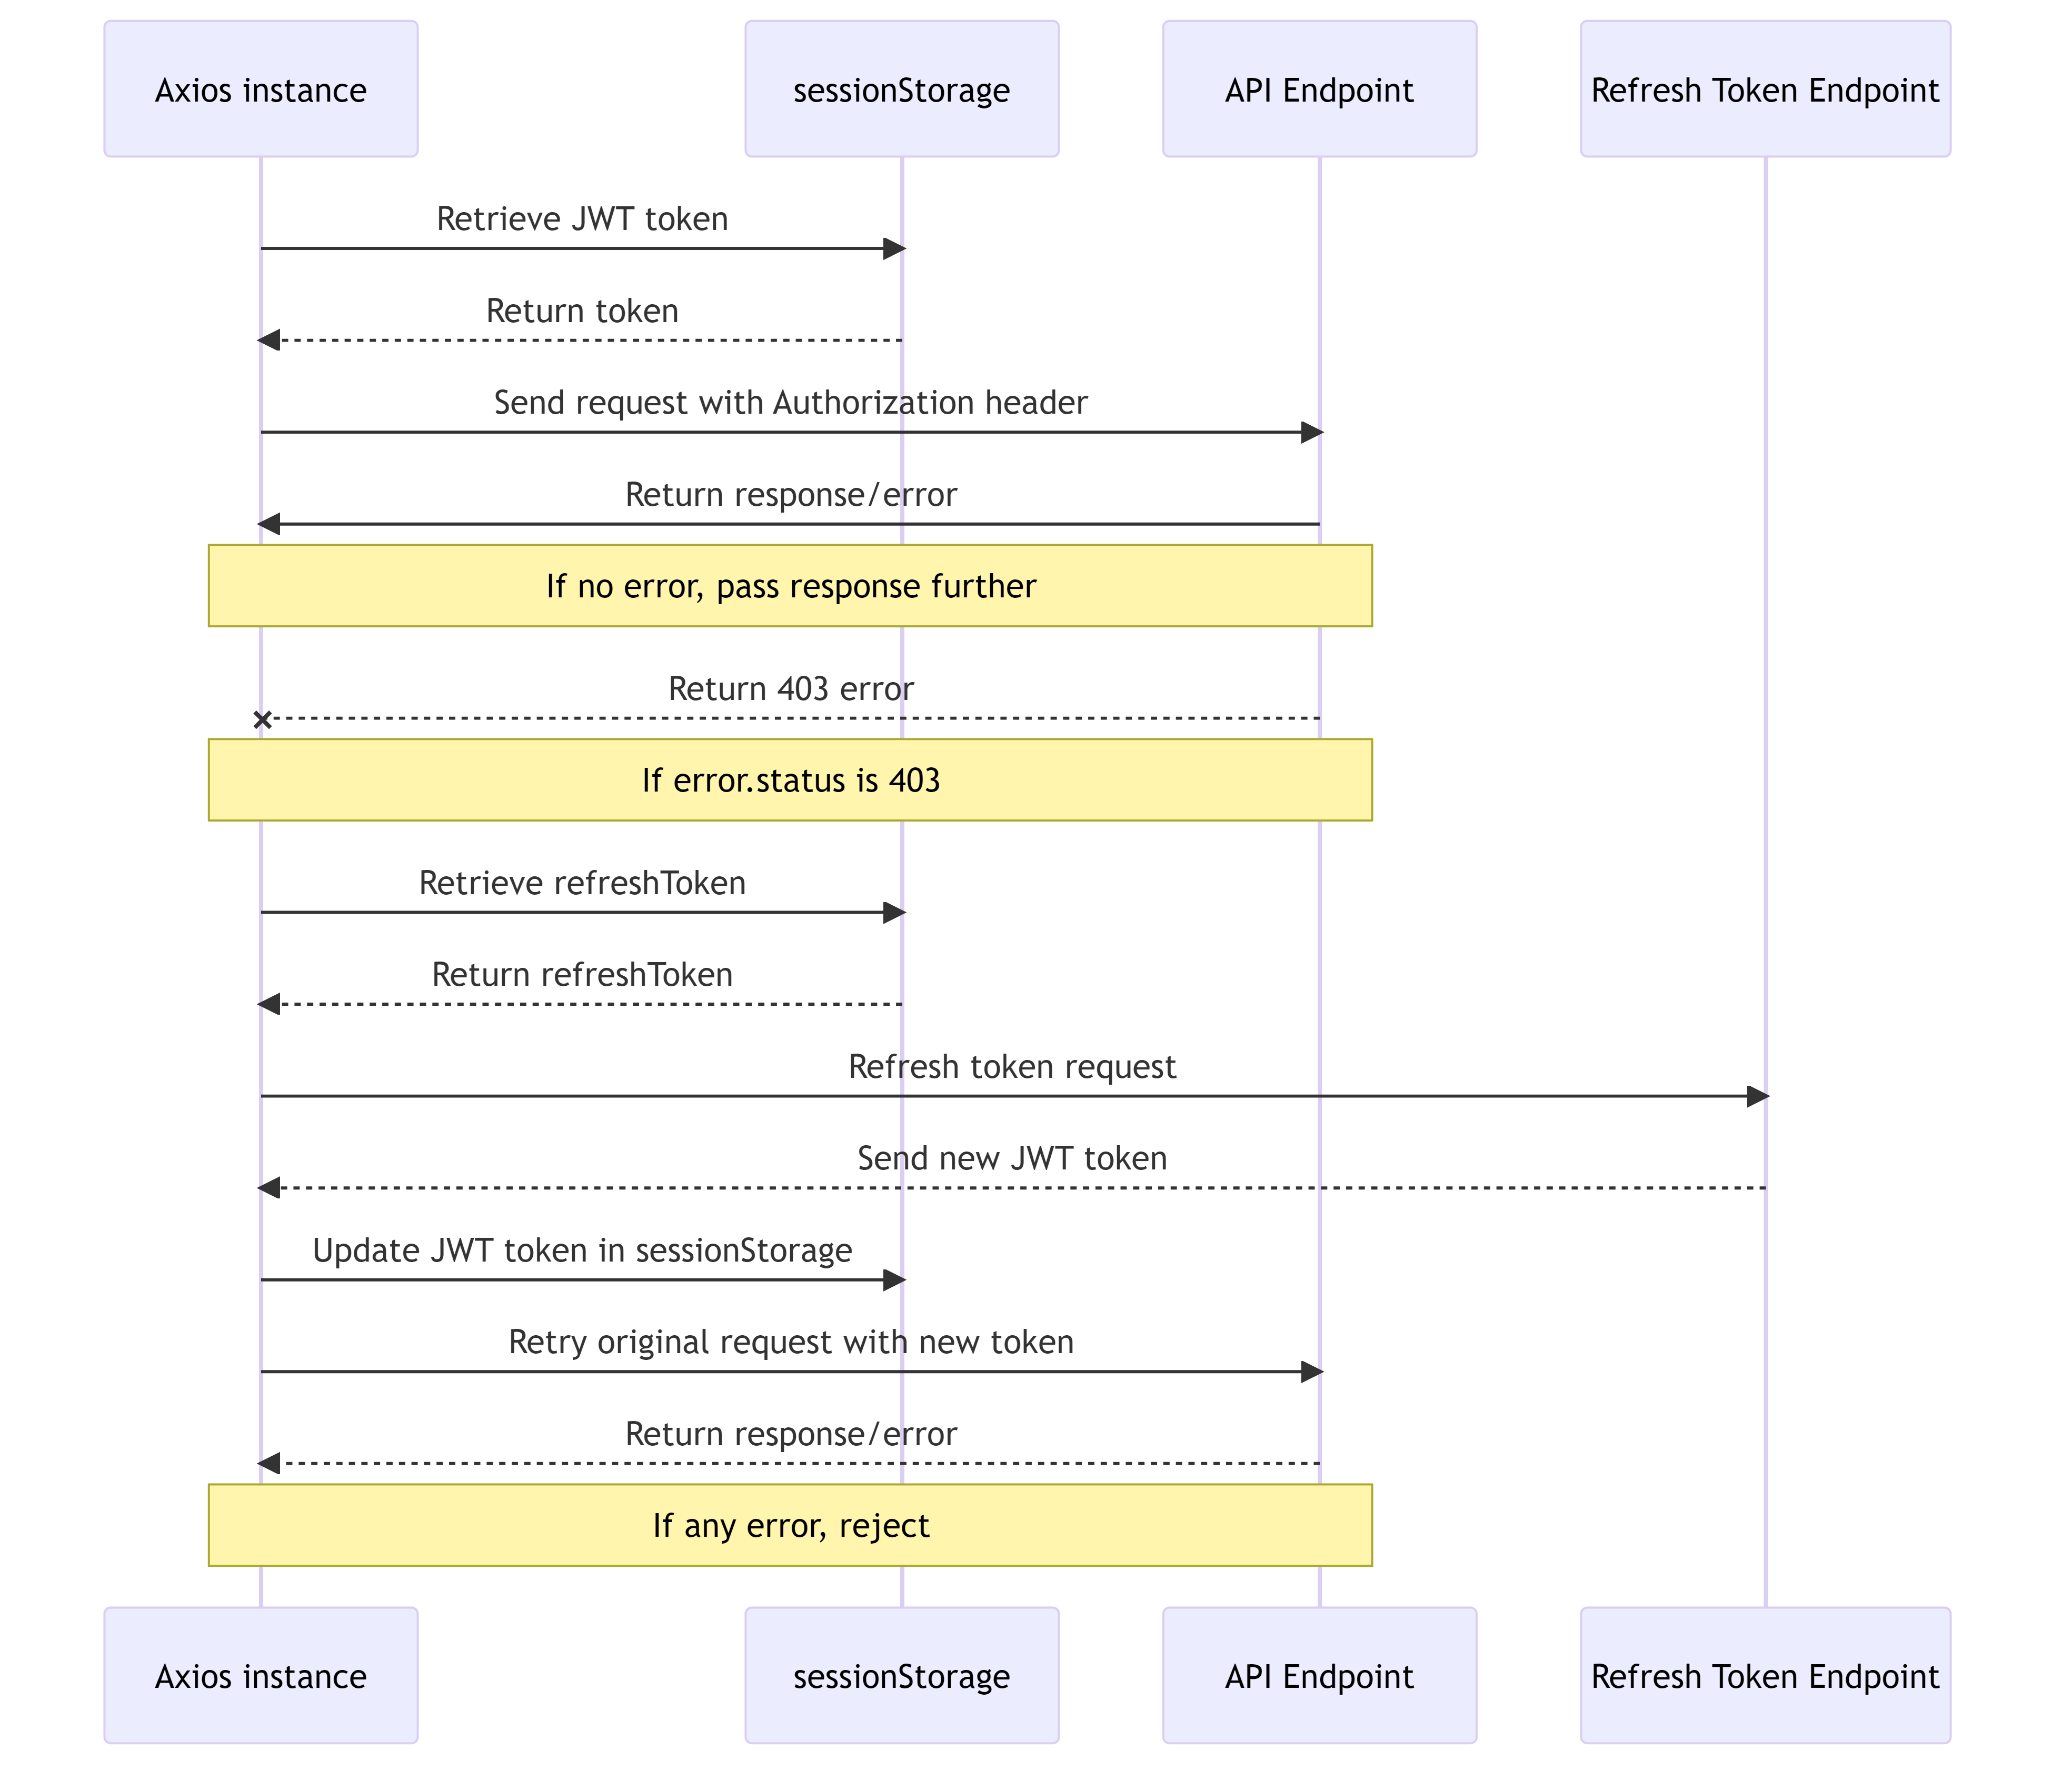
\includegraphics[width=1\linewidth]{includes/figures/axios.png}
    \caption{vereinfachter Ablauf des Sendens von Statusinformationen mittels eines eigenen EventServices}
\label{fig:react_axios}
\end{figure}

Zusätzlich erlaubt Axios die Implementierung von Interceptors. Diese überprüfen eingehende und ausgehende Requests auf ihren Status und ermöglichen eine direkte Verarbeitung. Das Konzept dahinter ist in Figur \ref{fig:react_axios} beschrieben. Fehlercodes wie '403 Not Allowed', 
die beispielsweise auftreten, wenn der JWT-Token abgelaufen ist, können durch einen separaten Refresh-Token erneuert werden, ohne dass eine erneute Anmeldung vom Nutzer erforderlich ist. Andere Fehlercodes kommen mit einem I18N-Fehlercodefeld aus dem Backend, 
um diese übersetzen zu können und so dem Nutzer genau anzuzeigen, was und warum etwas schiefgelaufen ist.


\subsection{Eingabenvalidierung über JSON Schema}
Nutzern die Eingabe möglichst einfach und verständlich zu gestalten und dabei auch Fehler zu vermeiden ist eine der wichtigsten Aufgaben eines angenehmen User Interfaces und trägt ungemein zur allgemeinen User Exerience bei.
Um dies dynamisch und flexibel zu erreichen, wurde eine Validierung der Eingaben von den ursprünglichen JsonForms durch rsjf\footnote{react-jsonschema-form ist ein react component, der ähnlich wie jsonforms, aus JSON Schemas React Components zusammenbaut} ersetzt. 
Diese überprüft die Eingaben auf ihre Korrektheit und gibt dem Nutzer ein visuelles Feedback, sollte etwas nicht stimmen. Im Gegensatz zur alten Variante aber erlaubt rsjf auch die Validierung von komplexeren Schemata und kann diese sogar in Kombination mit einer UI Definition darstellen.
Dies erlaubt es Validierung der Eingaben und Erstellung der UI zu verbinden und somit eine einheitliche und konsistente Darstellung zu gewährleisten.

 
Um die Felderbeschreibung und Fehlercodes zu übersetzen wurden Funktionen überschrieben welche das gesendete JsonSchema überschreiben und Fehlercodes sowie die dazugehörigen Argumente übersetzen. 
Dies erlaubt es dem Nutzer die Anwendung komplett in seiner eigenen Sprache zu nutzen und somit die User Experience zu verbessern.
Einen Nachteil hat dieses Vorgehen aber. Die Übersetzung der Beschreibungen setzt voraus, dass die Beschreibungen aus I18n Schlüsseln bestehen.
Fremde, oder neue User Interfaces, können die vom Backend bereitgestellten Schemata nur vernünftig darstellen, wenn diese die gleichen Schlüssel sowie Übersetzungsdateien verwenden.
Ohne eine Übersetztung ist nur der Schlüssel sichtbar, was für den Nutzer wenig hilfreich ist.

Ein weiterer großer Vorteil von rsjf ist die Möglichkeit, die Schemata dynamisch zu laden.
Anstatt wie bereits in Abschnitt \ref{sec:javaInputValidation} angedeutet die Schema fest im Code zu integrieren, was bedeutet hätte diese einzeln und für jeden Datentyp neu erstellen zu müssen, können diese durch das laden der Schema aus der API,
unabhängig vom Frontend erstellt werden und das Frontend muss lediglich eine Komponente zum laden, anzeigen und verarbeiten der Schemata bereitstellen.
Dies erleichterte besonders die Implementierung der "primitiven" Datentypen, da diese alle in der gleichen Komponente verarbeitet werden können.
Komplexere Schemata wie die der Machine Learning- und Zeit Serien Analyse Datentypen müssen aber weiterhin einzeln behandelt werden, da diese mehr Informationen benötigen als die "primitiven" Datentypen. 
Beide Datentypen verfügen über Auswahlmöglichkeiten zum genutzten Modell und dessen Konfiguration, die der Nutzer treffen muss. Diese werden in der UI als Dropdown Menüs dargestellt und in mehrere Schritte unterteilt, um die Mentale Belastung für den Nutzer möglichst gering zu halten.


\subsection{Bereitstellung von generischen Komponenten für Nutzerfeedback}
Feedback sollte konsistent sein. Egal bei welcher Aktion muss im Fehlerfall der Nutzer darüber benachtitigt werden.
MUI liefert hierfür bereits eine vorgefertigte Komponente und kann 4 verschiedene Feedbacks dem Nutzer geben.
Durch farbliche Unterscheidungen stellt es Informationen, Erfolgreiche Aktionen, Warnungen und Fehler dar. Dies natürlich in Kombination mit einer dazu passenden Erklärung.
Um diese Komponenten innerhalb der Gesammten App einzubauen wurde eine Wrapper Komponente geschrieben. 
Es erzwingt ein einheitliches Fehlerkonzept und vereinfacht die Nutzung. Da es sich um eine Austauschbare Komponente handelt, lässt sich diese später natürlich austauschen, erweitern und neuen Anforderungen anpassen.
Über die Zugabe von optionalen Übersetzungskeys ist die Fehleranzeige multilingual.
Es erlaubt damit eine einfache, dem Nutzer aus anderen Anwendungen bereits bekannte Lösung der in \ref{cha:Anforderungsanalyse:Usability} definierten Anforderung an eine Bereitstellung informativen Feedbacks.

\subsection{Bereitstellung von Mehrsprachigkeit durch i18n}
Fachsprache stellt, besonders für Nicht-Experten, eine grundlegende Herausforderung dar. Unabhängig von den Sprachkenntnissen einer Person, ist gerade die 
fachspezifische Terminologie oft schwierig zu verstehen. Nehmen wir beispielsweise Dieter Maibach, der seit vielen Jahren in einem deutschen Unternehmen arbeitet. 
Obwohl er Englisch sprechen kann, ist er nicht mit der englischen Fachsprache vertraut. Eine Software nur in einer Sprache anzubieten, die er nicht vollständig versteht, 
würde ihm erhebliche Schwierigkeiten bereiten. Eine Übersetzung der Anwendung wäre daher vorteilhaft.

Es gibt bereits zahlreiche Lösungen für dieses Problem. Im Bereich von React ist die i18next-Bibliothek weit verbreitet. Sie ermöglicht es, Anwendungen 
mithilfe von JSON-Dateien, in denen die Übersetzungen gespeichert sind, mehrsprachig zu gestalten. Der Nutzer hat dann zwei Optionen: Entweder wählt er die Sprache 
selbst aus, oder ein Detektor übernimmt die Spracheinstellung des Browsers. Eine I18N-Integration führt somit zu einer deutlich verbesserten Benutzererfahrung, da die 
Anwendung in der bevorzugten Sprache des Nutzers verwendet werden kann.

Es ist daher sinnvoll, dem Nutzer die Möglichkeit zu bieten, die Anwendung in seiner eigenen Sprache zu nutzen. Durch eine I18n-Integration kann die 
Anwendung ohne erheblichen Aufwand in verschiedene Sprachen übersetzt und somit die Benutzerfreundlichkeit erheblich gesteigert werden. Die Übersetzung der Texte 
erfolgt direkt im Frontend. Nutzer können ihre bevorzugte Sprache angeben; falls sie dies nicht tun, wird versucht, die Standardsprache des verwendeten Webbrowsers zu 
verwenden. Die Übersetzungen werden in JSON-Dateien innerhalb des Projekts gespeichert. Diese können dann über eine Komponente in die Anwendung geladen werden.

Etwas komplizierter gestaltete sich die Übersetzung der rsjf-Komponente. Da diese die Beschreibungen der Felder aus dem Schema lädt, müssen diese 
ebenfalls übersetzt werden. Ein speziell hierfür entwickelter Konverter liest das Schema aus. Anstatt mit normalen Beschreibungen zu arbeiten, mussten die 
Feldbeschreibungen als i18n-Schlüssel gespeichert werden. Dies gilt auch für die Fehlerbehandlung und -anzeige, die ebenfalls über ihre spezifischen Fehlercodes übersetzt werden müssen.
\begin{figure}[ht]
    \centering
    \begin{minipage}{0.5\textwidth}
        \centering
        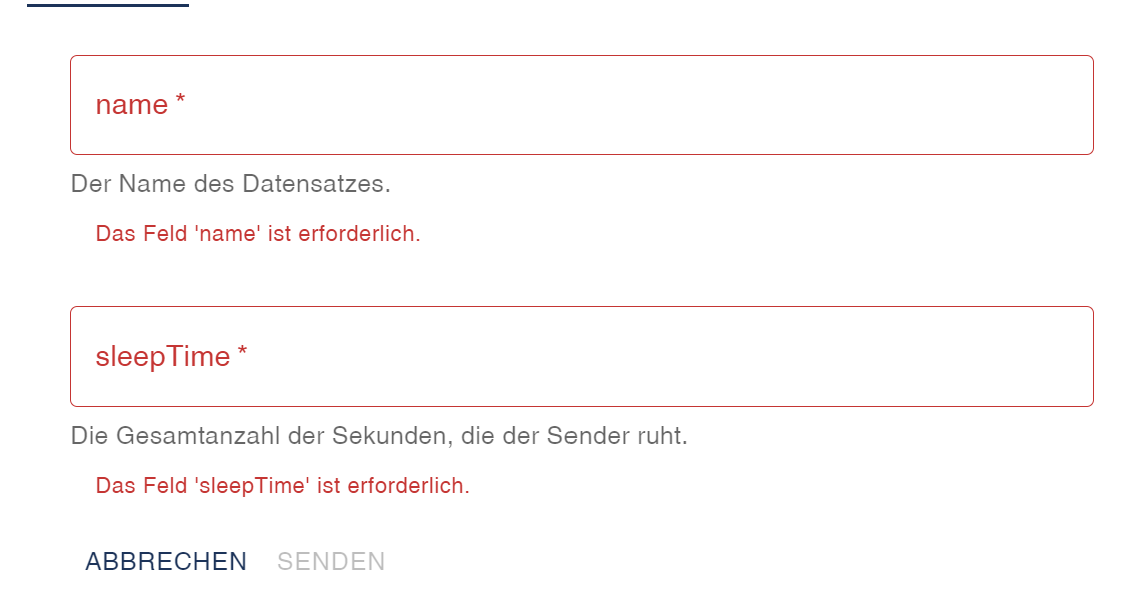
\includegraphics[width=\textwidth]{includes/figures/new_version/rsjf_translation_1.png}
        \caption{Analyse des CGAN tsgm Modells}
        \label{fig:rsjf_translation_1}
    \end{minipage}\hfill
    \begin{minipage}{0.5\textwidth}
        \centering
        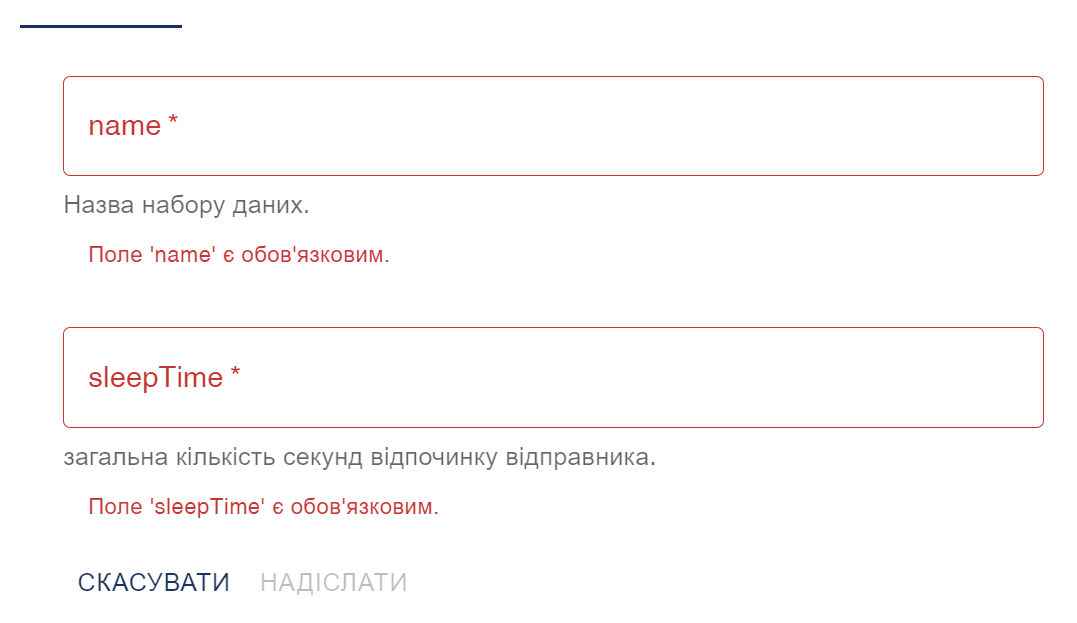
\includegraphics[width=\textwidth]{includes/figures/new_version/rsjf_translation_2.png}
        \caption{Analyse des CGAN Keras Modells}
        \label{fig:rsjf_translation_2}
    \end{minipage}
\end{figure}


\subsection{Websockets und Ihre Auswirkungen für den Nutzer}
Da, wie bereits in Spring erwähnt, es viele lang laufende Aufgaben gibt und diese für den Nutzer wenig Transparent sind, wurden in beiden APIs bereits Websocket-Endpunkte eingefügt um dem Nutzer dieses fehlende Feedback zu geben.
Diese jedoch zu implementieren stellte sich als deutlich komplexer heraus als anfangs angenommen. Security beider APIs und teilweise unterschiedlicher Protokolle, 
Zentralisierung und Verwaltung (Erstellen, auf Nachricht warten und Beenden der Verbindungen) der Websockets, das Serialisieren der Nachrichten und die multivariante Darstellung spielten hier alle mit rein.


Die Webapp muss mehrer Websockets gleichzeitig halten und verwalten können.
Nutzer können, sofern die Resourcen des Servers dies natürlich zulassen, gleichzeitig mehrere Modelle trainieren. Um es dem Nutzer hier so einfach wie möglich zu machen, hängt am Modell ein Forstschritt Element, welches numerisch und visuell den gesammten Forschritt zeigt.
Man kann aber nicht erwarten, dass der Nutzer auf der Seite des Modelles wartet, ob dieses bereits fertig trainiert ist oder noch läuft (siehe Abbildung \ref{fig:websocket_sending_projects}).
Hier kommt die zentrale Steuerung der Websockets ins Spiel. Über eine Drawer Komponente kann ein Live-Fortschritt des Modells überwacht werden. Dieses ist von jedem Punkt innerhalb der Anwendung erreichbar.
Nutzer können somit, ohne in ihrem Arbeitsfluss unterbrochen zu werden schauen, ob sie bereits neue Modelle starten können oder das trainierte Modell in ihre Tracks integrien können.
Ebendso gilt dies auch für die Projects welche gerade senden. Sollten mehrere verschiedene Projects gleichzeig senden und diese darüber hinaus auch mit zeitlich unterschiedlich langen Tracks, so kann der Nutzer dies nur schwer nachvollziehen, ohne eine Kafka Consumer implentation nebenbei laufen zu haben.
Die gleiche Drawer Komponente sorgt auch hier für klarheit, in dem sie den Fortschritt prozentual (auf die Anzahl der Tracks gerechnet) in einem Balkendiagramm anzeigzt.

\begin{figure}[h]
    \centering
    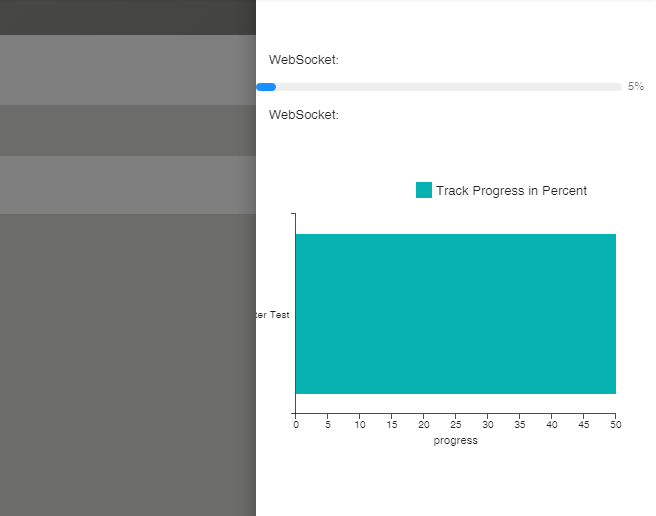
\includegraphics[width=0.9\linewidth]{includes/figures/new_version/websocket_model_training.png}
    \caption{Websocket Drawer für das Trainieren von Modellen und als Fortschrittsanzeige für sendende Projects}
\label{fig:websocket_sending_projects}
\end{figure}



\subsection{Konfiguration der Komponenten im Bereich machinelles Lernen}
Der Bereich des Machine Learnings in der Anwendung ist bewusst einfach gehalten, um eine intuitive Bedienung zu gewährleisten und Nutzer nicht mit, im Überblick unwichtigen Daten zu überlasten. Auch spiegelt dies das aktuelle \ac{API}-Design wieder, welches die Konfigurationen der Modelle über einen separaten Endpunkt verwaltet. 
Alle möglichen Konfigurationen werden beim Erstellen oder Aktualisieren des Modells vorgenommen. Diese Entscheidung basiert auf einem wichtigen Grund: 
Wie bereits in Abschnitt \ref{sec:djangoML} erörtert, stellt das Training von Modellen ein komplexes Unterfangen dar. Eine Vielzahl an Nutzereingaben kann insbesondere für fachfremde Benutzer mental anstrengend sein. 
Um den Prozess zu vereinfachen, wurde der Dialog in verschiedene, abgeschlossene Teile gegliedert. Dies reduziert die kognitive Belastung für den Benutzer. 
Im ersten Schritt gibt der Nutzer lediglich grundlegende Daten wie Namen und Beschreibung ein. Anschließend werden im nächsten Schritt die Trainingsdaten ausgewählt. Hierfür hat der Nutzer mehrere Möglichkeiten.
Wie in vielen Anwendungen bereits bekannt, gibt es eine Fläche, in die Daten über das Drag'n'Drop Prinzip abgelegt werden, alternativ wird ein Dialog zur manuellen Suchen geöffnet. 
Dann besteht noch die Möglichkeit zwischen Dateien und Elementen innerhalb der Datein zu wählen. Dieses Konzept wurde gewählt, da gerade größere CSV Dateien eine Vielzahl an Spalten enthalten können und es für den Nutzer einfacher ist, die Daten direkt in der Anwendung zu filtern, als dies in einer externen Anwendung zu tun.
Der letzte Schritt beinhaltet die spezifischen Konfigurationen für das Training des Modells. Durch ein strukturiertes und dynamisch angepasstes Eingabefeld kann der Nutzer die verschiedenen Optionen prüfen und, sofern die Daten bereits hochgeladen sind, sich einen Überblick über die Auswirkungen seiner Auswahl verschaffen. 
Der dargestellte Graph vergleicht eine originale Datei mit ihrer nach der Konfiguration bearbeiteten Version (Siehe Abbildung \ref{fig:configuration_graph_overview}) und, sofern die Zeitreihe nicht vollständig ist, zeigt auch den Unterschied der verwendeten Imputationsalgorithmen. Da dieser Prozess rechenintensiv ist, wird er nicht für alle Zeitreihen angeboten und ist nur im Dialog zu finden.

\begin{figure}[h]
    \centering
    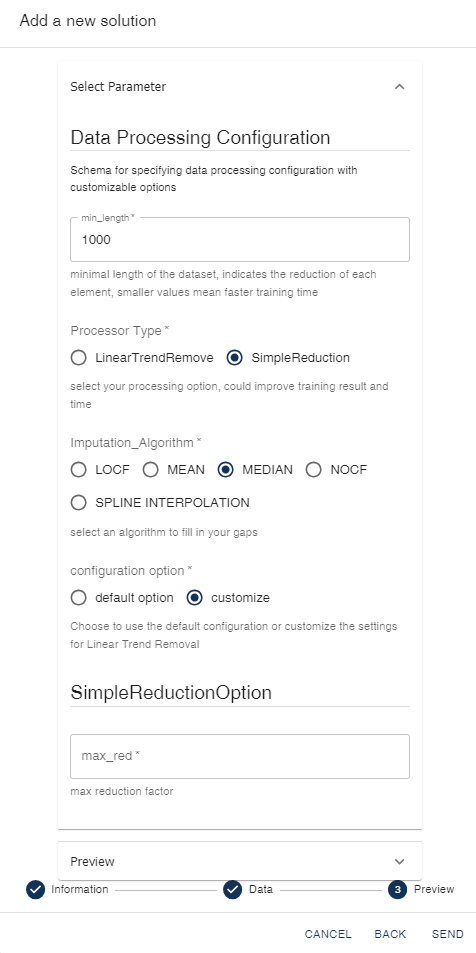
\includegraphics[width=0.5\textheight]{includes/figures/new_version/data_processing.png}
    \caption{Eingeabefeld für die Datenvorverarbeitung sowohl für die Zeit Serien Analyse als auch für das maschinelle Lernen}
\label{fig:configuration_json_schema}
\end{figure}


\begin{figure}[ht]
    \centering
    \begin{minipage}{0.5\textwidth}
        \centering
        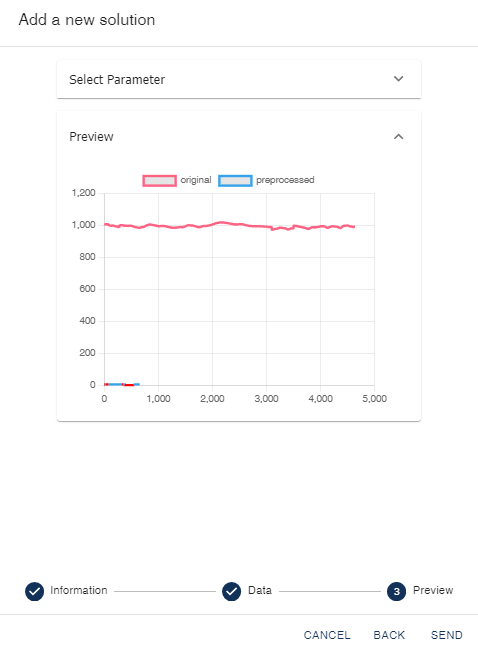
\includegraphics[width=\linewidth]{includes/figures/new_version/data_processing_2.png}
        \caption{Eingeabefeld für die Datenvorverarbeitung sowohl für die Zeit Serien Analyse als auch für das maschinelle Lernen, hier können grafisch die Unterschhiede zwischen den Originaldaten und den verarbeiteten Daten interaktive angesehen werden.}
        \label{fig:configuration_graph_overview}
    \end{minipage}\hfill
    \begin{minipage}{0.5\textwidth}
        \centering
        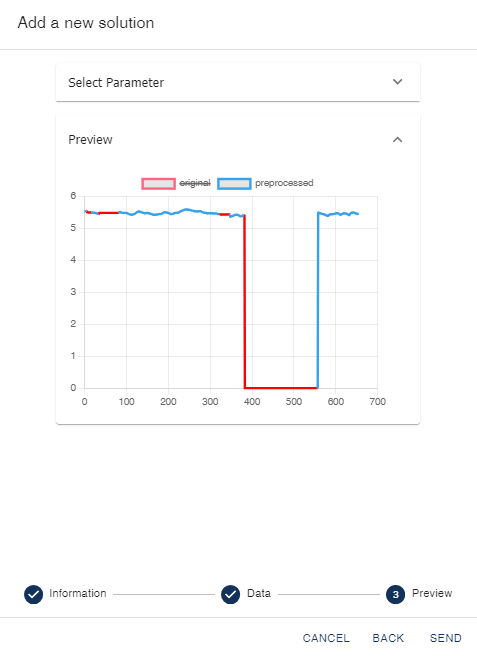
\includegraphics[width=\linewidth]{includes/figures/new_version/data_processing_3.png}
        \caption{In diesem Beispiel werden die originalen Daten ausgeblendet. Die roten Bereiche sind fehlende Werte, welche durch den Imputationsalgorithmus ersetzt wurden. Die große Lücke in der Mitte ist zu groß und wird nicht ersetzt, sondern durch ein ML Modell gefüllt.}
        \label{fig:configuration_graph_overview2}
    \end{minipage}
\end{figure}




In der Hauptansicht hat der Nutzer Zugriff auf mehrere wichtige Komponenten. Er kann seine Beschreibungen einsehen, was insbesondere bei einer Vielzahl an Modellen sehr hilfreich ist. 
Zudem bietet die Anwendung eine Übersicht, in welchen Projekten das Modell bereits eingesetzt wird, und ermöglicht einen direkten Zugriff auf diese. Weiterhin kann der Nutzer sein Modell starten und dabei einige Optionen festlegen, 
die den Trainingsverlauf wesentlich beeinflussen. Hat der Nutzer ein Modell bereits trainiert, erhält er eine Übersicht mit allen relevanten Trainingsinformationen, einschließlich Datum, Laufzeit und einem Beispielbild (Siehe Abbildung \ref{fig:ml_trained_configuration}). Dieses zeigt im direkten Vergleich die Ausgabe des Modells im Vergleich zu einem Element aus dem Trainingsdatensatz. Sollte das Ergebnis nicht den Erwartungen entsprechen, erkennt der Nutzer dies sofort und hat die Möglichkeit, das Modell mit neuen Parametern erneut zu trainieren
\begin{figure}[h]
    \centering
    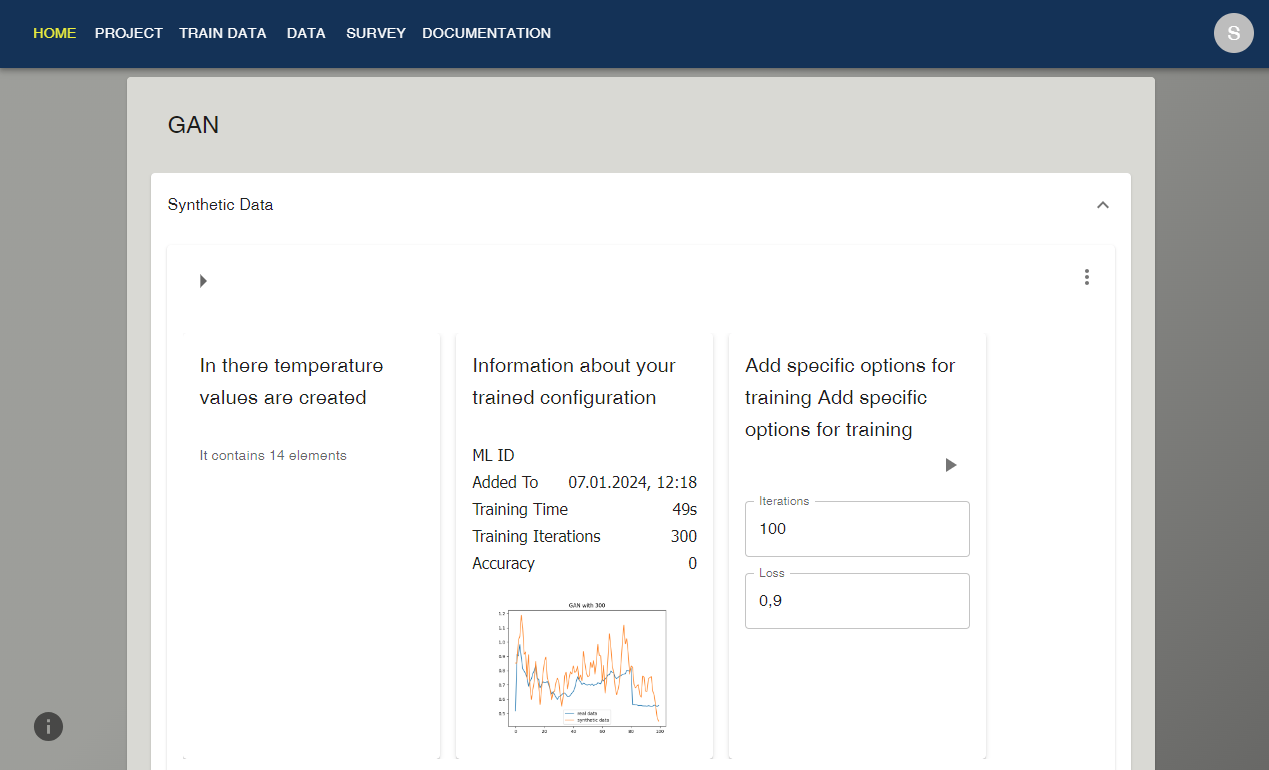
\includegraphics[width=0.9\linewidth]{includes/figures/new_version/ml_configuration.png}
    \caption{Ansicht eines trainierten Modells mit den wichtigsten Informationen und einem Beispielbild}
\label{fig:ml_trained_configuration}
\end{figure}

Zugriff auf interne Parameter der Modelle ist nicht möglich. Dies ist eine bewusste Entscheidung, um die Komplexität der Anwendung zu reduzieren und die Benutzerfreundlichkeit zu erhöhen. Es könnte durch die API angeboten werden, 
bedarf aber eines enormen Valididerungsaufwandes, da die Parameter je nach Modell stark variieren, freie Kombinationen meist nicht funktionieren und eine vernünftige \ac{API} Dokumentation hierfür enorm aufwändig wäre.

\subsection{Konfiguration der Komponenten im Bereich der Zeitreihenanalyse}
\label{sec:reactTSA}
Der Bereich der Zeitreihenanalyse ist ähnlich konzipiert wie der des Machine Learnings. Auch hier wurde Wert darauf gelegt, dieselben Komponenten zu verwenden, um den Nutzern eine konsistente und einheitliche Erfahrung zu bieten. 
Der Dialog zur Erstellung und Aktualisierung einer Konfiguration für ein Modell ist ebenfalls in mehrere Schritte unterteilt. Zunächst werden spezifische Daten für die Konfiguration eingegeben. Im zweiten Schritt erfolgt die Auswahl oder das Hochladen der Trainingsdaten. 
Im letzten Schritt kann der Nutzer die Verarbeitung der Daten anpassen, genau wie es auch in den Abbildungen \ref{fig:configuration_json_schema} und \ref{fig:configuration_graph_overview} zu sehen ist.

Ein wesentlicher Unterschied zum maschinellen Lernen besteht darin, dass die Nutzer die Modelle hier nicht trainieren müssen. Die Operationen werden direkt auf die Daten angewendet, und das Ergebnis wird dem Nutzer in verschiedenen Grafiken dargestellt. 
Bei Methoden wie der Singulärwertzerlegung (\ac{SSA}) und der empirischen Moduszerlegung (\ac{EMD}), bei denen das Signal zuerst in mehrere intrinsische Modenfunktionen (\acp{IMF}) zerlegt wird, erhält der Nutzer eine Übersicht über die einzelnen \acp{IMF}. 
Zusätzlich gibt es die Möglichkeit, diese zu verschieben, um das Ergebnis zu beeinflussen (siehe Abbildung \ref{fig:tsa_trained_configuration}). Dies kann nützlich sein, um beispielsweise Phasen zu verschieben, obwohl es kein Bestandteil der späteren Analyse ist.

Methoden wie AMIRA, die grundlegend anders funktionieren, präsentieren lediglich einen Graphen, der das Ergebnis in Arbeitsform zeigt. Dies dient dazu, die Menge der Daten, die regelmäßig zwischen der API ausgetauscht werden müssen, zu reduzieren.
\begin{figure}[h]
    \centering
    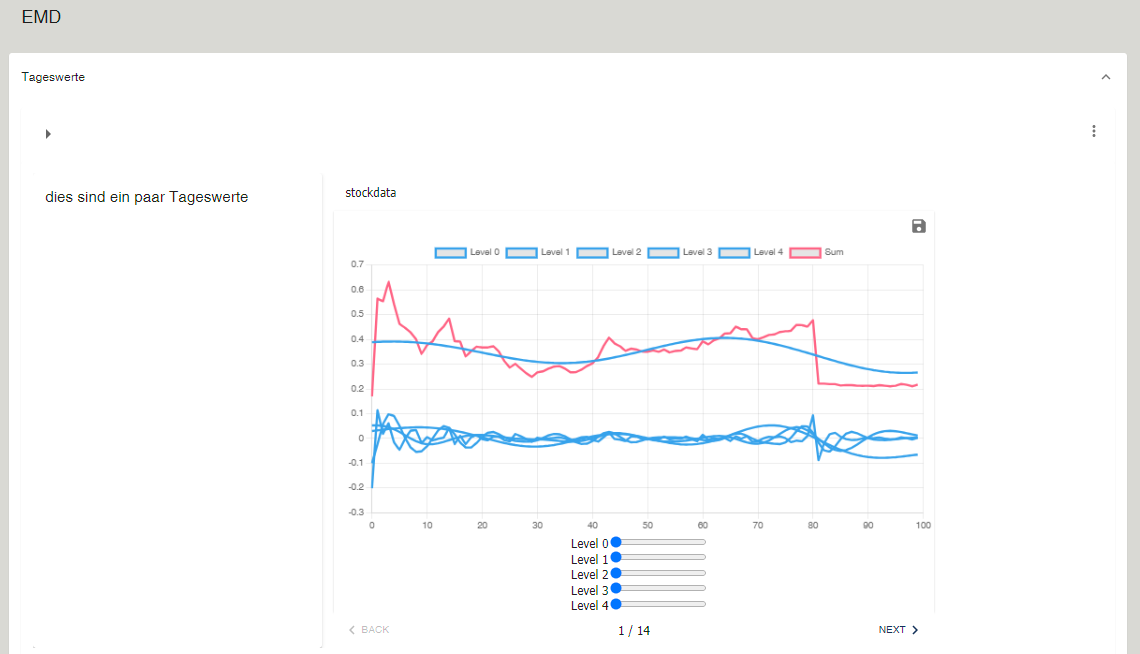
\includegraphics[width=0.9\linewidth]{includes/figures/new_version/tsa_configuration.png}
    \caption{Ansicht einer Zeitreihenzerlegung über den \ac{EMD} Algorithmus}
\label{fig:tsa_trained_configuration}
\end{figure}

Änderungen an den Modellen können nur über den Aktualisierungsdialog vorgenommen werden, indem die Konfiguration angepasst wird.
Dies ist eine bewusste Entscheidung, um die Komplexität der Anwendung zu reduzieren, da die ganzen Informationen nicht überwältigend wirken. Auch räumt es die Ansicht auf und konzentriert den Fokus auf die einzelnen Zeitreihen.
Informationen wie Laufzeit und Datum des letzten Trainings, wie es beispielsweise bei den \ac{ML} Modellen der Fall ist, ist hier nicht relevant, da die Daten in fast Echtzeit bereitgestellt werden können.

\subsection{Verwalten der hochgeladenen Daten}
Zugriff und Verwaltung der Trainingsdaten ist, wie bereits im Kaptiel \ref{cha:Anforderungsanalyse:Datenmanagement} beschrieben, ein wichtiger Bestandteil der Anwendung.
Da in den meisten Fällen Daten innerhalb der Dialoge beim Erstellen neuer Machine Learning und Time Series Analysis Konfigurationen hochgeladen werden, ist es wichtig dem Nutzer eine Möglichkeit zu bieten diese Daten auch zu verwalten.
Gerade bei komplexeren Datein, wie sie CSV Dateien mit vielen Spalten produzieren, ist ein visuelles Feedback durchaus praktisch.
Sollten Daten, oder Graphen, nicht in das gewünschte Konzept passen, kann der Nutzer diese auch direkt aus der Datei entfernen. Dies ist aber nur möglich, sofern die spezifische Datei nicht an eine Konfiguration gebunden ist.
Direkt werden dem Nutzer nur seine Datein angezeigt (Siehe Abbildung \ref{fig:data_overview_files}). Die einzelnen Graphen werden erst geladen, wenn die Datei ausgeklappt wird. Somit wird die Auslasung etwas reduziert und die Anwendung läuft flüssiger.

\begin{figure}[h]
    \centering
    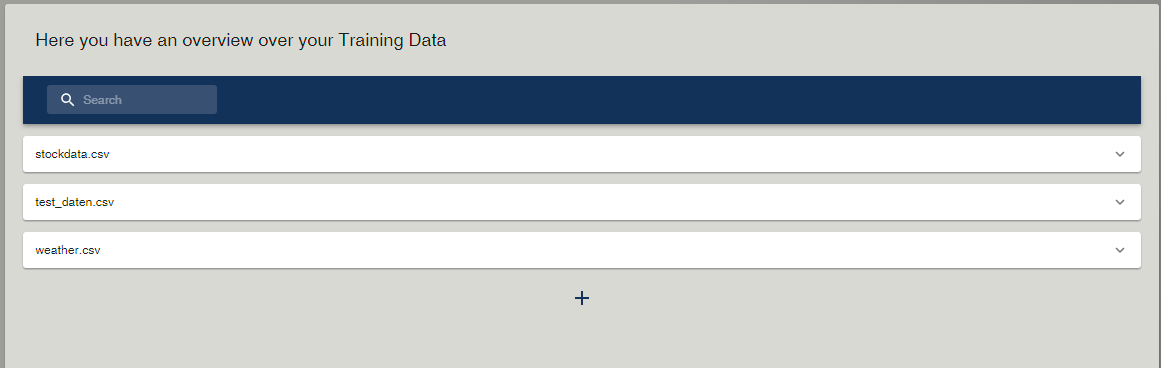
\includegraphics[width=0.9\linewidth]{includes/figures/new_version/data_overview.png}
    \caption{Übersicht über die hochgeladenen Datein und deren Inhalte}
\label{fig:data_overview_files}
\end{figure}
% !TeX program = xelatex

\chapter{Aufbau der Testumgebung}
\label{sec:testing}

\section{Metriken und Methoden der Testumgebung}
\label{sec:test_framework}

In den Abschnitten \ref{sec:djangoML} und \ref{sec:djangoTSA} wurde bereits auf die grundlegende Implementierung der Modelle oder Algorithmen beider Varianten in Grundzügen eingegangen. 
In diesem Abschnitt wird nun die Implementierung des Testframeworks beschrieben, das die beiden Varianten vergleicht.

Dies ist nicht trivial, da die Kriterien für synthetische Daten im Vergleich zu ihrem realen Pendant auf Ähnlichkeit, jedoch bewusst nicht auf Identität beruhen. 
Eine einfache euklidische Distanzberechnung ist daher nicht sinnvoll. Stattdessen wird auf verschiedene Methoden zurückgegriffen, die im Folgenden beschrieben werden.


\subsection{Nicht-Statistische Maße}
\label{sec:non_statistical_measures}

\paragraph{Wasserstein-Distanz}
Die Wasserstein-Distanz, auch als Earth Mover's Distance\cite{Understa51:online} bekannt, ist hilfreich, um Unterschiede zwischen zwei Wahrscheinlichkeitsverteilungen zu quantifizieren. 
Im Gegensatz zur euklidischen Distanz, bei der die direkten Differenzen zwischen einzelnen Datenpunkten berechnet werden, berücksichtigt die Wasserstein-Distanz die gesamte Struktur der Verteilungen. 
Somit ist sie als Metrik in Szenarien, in denen nicht nur identische, sondern ähnliche Daten verglichen werden, durchaus aussagekräftig.

\begin{equation}[Wasserstein-Distanz]
    \label{eq:wasserstein_distance}
    W_p(\mu, \nu) = \left( \inf_{\gamma \in \Gamma(\mu, \nu)} \int_{M \times M} d(x, y)^p \, d\gamma(x, y) \right)^{\frac{1}{p}}
\end{equation}

Für die in Gleichung \ref{eq:wasserstein_distance} verwendeten Variablen gilt:

\(W_p(\mu, \nu)\) ist die Distanz zwischen den beiden Verteilungen \(\mu\) und \(\nu\), \(\Gamma(\mu, \nu)\) die Menge aller Kopplungen zwischen \(\mu\) und \(\nu\) und \(d(x, y)\) ist die euklidische Distanz zwischen x und y.

Speziell in der Zeitreihenanalyse ist dies besonders relevant, da synthetische Zeitreihen im Vergleich zum Original Verschiebungen aufweisen können. 
Die Wasserstein-Distanz kann solche Verschiebungen handhaben, da sie die gesamte Verteilung der Datenpunkte berücksichtigt, anstatt eines Punkt-zu-Punkt-Vergleichs wie bei der euklidischen Distanz.

Sofern die Trainingsdaten jedoch eine zu heterogene Verteilung aufweisen, ist die Wasserstein-Distanz wenig geeignet, 
da ihre Aussagekraft zu unterschiedlich sein kann. Dies ist bei variablen Daten grundsätzlich der Fall, da die Daten nicht nur unterschiedliche Werte, 
sondern auch unterschiedliche Verteilungen aufweisen können. Als Metrik für vorher bekannte Daten ist die Wasserstein-Distanz jedoch durchaus geeignet.

\paragraph{Autokorrelation}
Eine weitere Methode ist die Analyse der Autokorrelation\cite{statistikguru} innerhalb von Zeitreihen. 
Die \acf{ACF} misst, wie stark eine Zeitreihe mit verzögerten Versionen von sich selbst korreliert ist. 
Dies ist besonders nützlich, um die interne Struktur von Zeitreihendaten zu verstehen, insbesondere im Hinblick auf ihre Periodizität und saisonale Muster.

\begin{equation}
    \label{eq:autocorrelation}
    ACF(k) = \frac{\sum_{t=1}^{n-k} (X_t - \overline{X})(X_{t+k} - \overline{X})}{\sum_{t=1}^{n} (X_t - \overline{X})^2}
\end{equation}

In Gleichung \ref{eq:autocorrelation} repräsentiert \( ACF(k) \) die Autokorrelation zum Lag \( k \), \( X_t \) ist der Wert der Zeitreihe zum Zeitpunkt \( t \), und \( \overline{X} \) ist der Mittelwert der Zeitreihe. 
Diese Funktion hilft dabei, Periodizitäten und wiederkehrende Muster in den Daten zu identifizieren, die für die Prognose und Analyse zukünftiger Datenpunkte nützlich sein können.

\paragraph{Fourier-Transformation}
Ein weiteres wichtiges Maß ist die Spektralanalyse, die Frequenzkomponenten einer Zeitreihe identifiziert. 
Hierfür kann der \acf{FFT} Algorihtmus genutzt werden, um Zeitreihen von einer Zeit- in eine Frequenzdomäne zu überführen, um so dominierender Frequenzen und periodischer Signale in den Daten zu identifizieren \cite{szeliski2011computer}.

\begin{equation}
    \label{eq:fourier_transform}
    F(\omega) = \int_{-\infty}^{\infty} f(t) e^{-2\pi i \omega t} \, dt
\end{equation}

In Gleichung \ref{eq:fourier_transform} ist \( F(\omega) \) die Fourier-Transformierte der Zeitreihe \( f(t) \), wobei \( \omega \) die Frequenz und \( t \) die Zeit darstellt. 
Diese Analyse ist besonders wertvoll, um zyklische Verhaltensweisen in Zeitreihendaten zu erkennen, die durch einfache Abstandsmetriken nicht erfasst werden können.


\subsection{Statistische Maße}
\label{sec:statistical_measures}
Zeitreihen, wie alle Datensätze, folgen spezifischen Verteilungen. Wenn man annimmt, dass die originalen Daten einer bestimmten Verteilung folgen, 
sollten die synthetischen Daten diese Verteilung widerspiegeln. Daher kann der Einsatz statistischer Methoden zur Bewertung der Ähnlichkeit zwischen synthetischen und realen Daten als aussagekräftig angenommen werden. 
Dies gilt insbesondere, wenn man davon ausgeht, dass die synthetischen Daten zwar nicht identisch, aber statistisch ähnlich zu den realen Daten sein sollen. 

\paragraph{Kullback-Leibler Divergenz}
Ein wichtiges statistisches Maß in diesem Kontext ist die \acf{KLD} (siehe \cite{Kullback98:online}). Die \ac{KLD} quantifiziert den Informationsverlust, der auftritt, wenn eine Verteilung genutzt wird, um eine andere Verteilung anzunähern. 
Ein hoher Wert der KLD signalisiert erhebliche Unterschiede zwischen den Verteilungen, was darauf hinweist, dass die synthetischen Daten die realen nicht adäquat abbilden und wichtige Informationen verloren gehen. 
Im Gegensatz dazu indiziert ein niedriger KLD-Wert eine starke Ähnlichkeit der Verteilungen, was nahelegt, dass die synthetischen Daten eine präzise Repräsentation der realen Daten sind und der Informationsverlust minimiert ist
Mathematisch ist es definiert als:

\begin{equation}
    \label{eq:kl_divergence}
    D_{KL}(P || Q) = \sum_{i} P(i) \log \left( \frac{P(i)}{Q(i)} \right)
\end{equation}

Wobei \(D_{KL}(P || Q)\) die Kullback-Leibler Divergenz zwischen den Verteilungen P und Q ist. 
\(P(i)\) und \(Q(i)\) sind die Wahrscheinlichkeiten für das Ereignis \(i\) in den Verteilungen P und Q.


\paragraph{Maximum Mittelwert Diskrepanz}
\textit{\acf{MMD}} ist eine nicht-parametrische Methode, die Unterschiede zwischen zwei Verteilungen auf Basis von Stichproben aus jenen Verteilungen evaluiert.
Definiert ist sie über:

\begin{equation}
    \text{MMD}^2(P, Q) = \mathbb{E}_{x,x' \sim P}[k(x, x')] + \mathbb{E}_{y,y' \sim Q}[k(y, y')] - 2\mathbb{E}_{x \sim P, y \sim Q}[k(x, y)]
\end{equation}
Wobei, wie in Formel \ref{eq:kl_divergence} bereits definiert, \(P\) und \(Q\) die beiden Verteilungen sind, \(x,x'\) und \(y,y'\) sind die jeweiligen Stichproben und \(\mathbb{E}\) der Erwartungswert.

Sie verwendet eine Kernel-Funktion \(k\), um die Distanz zwischen den Mittelwerten beider Verteilungen im Feature-Raum zu messen. 
Da sie keinerlei Annahmen über die Form der Verteilungen macht, ist \ac{MMD} ein flexibles Werkzeug zur Analyse, insbesondere wenn die Form der Verteilungen unbekannt oder komplex ist, wovon bei variablen Datensätzen grundsätzlich auszugehen ist.
Es eignet sich daher sehr gut, um festzustellen, ob zwei Stichproben aus der gleichen Verteilung stammen, was in vielen Anwendungen der Zeitreihenanalyse von Bedeutung ist.


\paragraph{Mann-Whitney-U-Test}
Der Mann-Whitney-U-Test, auch bekannt als Wilcoxon-Rangsummentest, ist ein nicht-parametrischer Test, der verwendet wird, um zu beurteilen, ob zwei unabhängige Stichproben aus identischen Populationen stammen. Der Test ist besonders geeignet für Daten mit unbekannter oder nicht-normaler Verteilung. Er vergleicht die Rangwerte der Daten in den beiden Gruppen.

Sei \( U \) die Teststatistik, die wie folgt berechnet wird:
\begin{equation}
    U = R_1 - \frac{n_1(n_1+1)}{2}
\end{equation}
wobei \( R_1 \) die Summe der Ränge in der ersten Gruppe, \( n_1 \) die Anzahl der Beobachtungen in der ersten Gruppe ist. Der Wert von \( U \) wird dann verwendet, um die Signifikanz des Unterschieds zwischen den beiden Gruppen zu beurteilen.

\paragraph{T-Test}
Der T-Test ist ein statistischer Hypothesentest, der verwendet wird, um zu prüfen, ob sich die Mittelwerte zweier Gruppen signifikant unterscheiden. Er setzt voraus, dass die Daten normalverteilt sind. Der unabhängige T-Test für zwei Gruppen ist definiert als:

\begin{equation}
    t = \frac{\bar{X}_1 - \bar{X}_2}{\sqrt{\frac{s_1^2}{n_1} + \frac{s_2^2}{n_2}}}
\end{equation}
wobei \( \bar{X}_1 \) und \( \bar{X}_2 \) die Mittelwerte der beiden Gruppen, \( s_1^2 \) und \( s_2^2 \) die Varianzen der Gruppen und \( n_1 \) und \( n_2 \) die Anzahl der Beobachtungen in den Gruppen sind. Der berechnete t-Wert wird dann mit einem kritischen Wert aus der T-Verteilung verglichen, um die Hypothese zu testen.




\subsection{Evaluation durch machinenelles Lernen}
\label{sec:ml_methods_evaluation}
Machine Learning-Algorithmen sind besonders effizient darin, Muster in Daten zu erkennen. Insbesondere die Diskriminatoren in generativen Modellen sind 
darauf ausgelegt zu beurteilen, ob die vom Generator erzeugten Daten realistisch sind oder nicht. 
Daher bietet sich die Genauigkeit des Diskriminators als Maß für die Ähnlichkeit zwischen synthetischen und realen Daten an. Wenn der Diskriminator die 
synthetischen Daten als real einstuft, deutet dies auf eine hohe Ähnlichkeit oder grundsätzlich gleiche Muster mit den tatsächlichen Daten hin.

Eine in der Wissenschaft verbreitete und oft genutzte Methode baut auf dem Konzept auf und erweitert dieses um dieses Konzept im Kontext der Privatsphäre und ethischer 
Aspekten synthetischer Daten, insbesondere personenbezogener Daten, anzuwenden. 
Ein Ansatz zur Bewertung des Datenschutzes ist die Überprüfung der Outputs eines trainierten Modells auf Ähnlichkeiten, die Rückschlüsse auf die ursprünglich verwendeten Trainingsdaten zulassen könnten. 
In dem Paper 'User-Level Membership Inference Attack against Metric Embedding Learning' von Guoyao Li, Shahbaz Rezaei und Xin Liu \cite{li2022userlevel} wird eine solche Methodik vorgestellt. 
Wenn ein Angreifermodell auf der Basis von synthetischen Daten trainiert wird und eine hohe Wahrscheinlichkeit besteht, dass dieses Modell die realen Trainingsdaten identifiziert, ist die Privatsphäre der Daten möglicherweise gefährdet. 
Dieses Konzept wurde beispielsweise von Nikitin et al. in \cite{nikitin2023tsgm} untersucht.

Ein weiterer wichtiger Aspekt ist die Erkennung von Ausreißern in den Daten. Wenn die realen Daten signifikante Anteile von Ausreißern aufweisen, sollten diese auch in den synthetischen Daten vorhanden sein. 
Zur Bewertung dieser Eigenschaft kann ein Random-Forest-Algorithmus eingesetzt werden, der auf den realen Daten trainiert wird und sowohl auf die realen als auch auf die synthetischen Daten angewendet wird. 
Eine ähnliche Verteilung von Ausreißern in beiden Datensätzen kann darauf hindeuten, dass die synthetischen Daten die extrema der realen Daten gut nachbilden.



\section{Bewertung der Methoden}
\label{sec:method_evaluation}
All diese Methoden wurden in einem Testframework implementiert,
Dieses Framework besitzt die reduzierten und leicht modifizierten Algorithmen, die auch in der \ac{API} verwendet werden. Es trainiert die Modelle sowie speichert deren Laufzeit und die von ihm generierten synthetischen Daten.

\begin{lstlisting}[language=Python, caption={Methode um Statistiken aus den generierten Daten zu erstellen}, label={code:testFramework_statistics}]
def run_test_for_synthetic_data(data, syn_date_file_name, filename="statistic"):
    syn_data = load_processed_data(syn_date_file_name)
    result = {}
    for i in syn_data.keys():
        result[i] = {}
        if len(syn_data[i]) == 99:
            x, y = build_summed_version(data), np.array(syn_data[i][0])
        else:
            x, y = build_summed_version(data), np.array(syn_data[i][0])
        result[i]["statistic"] = run_static_tests(x, y)
        result[i]["outlier"] = outlier_detection(data, y)
        result[i]["attacker"] = run_syn_analyzer_(data, syn_data[i])
        result[i]["kl"] = run_kullback_leibler_divergence(x, y)
    write_to_file(f"data/{filename}.json", result)
\end{lstlisting}


Abgespeichert werden die Daten in einer JSON Datei, welche dann von den verschiedenen Methoden gelesen werden kann.
Eine Methode nimmt dann die gesammelten Daten und wertet diese in verschiedenen Schritten aus und erstellt die notwendigen Statistiken (Siehe Listing \ref{code:testFramework_statistics}).
Da sie am Ende des Prozesses wieder gespeichert werden, können sie zu einem späteren Zeitpunkt analysiert und geplottet werden.


Im letzten Schritt werden die Daten dann an einen Clustering Algorithmus übergeben, welcher die Daten in verschiedene Gruppen unterteilt.
Über Pyplot\footnote{https://matplotlib.org/stable/tutorials/pyplot.html} können die Daten visualisiert werden und sind somit leichter zu bewerten.
Für die Clustering Methoden wurde Plotly\footnote{https://plotly.com/} verwendet, da diese eine interaktive Visualisierung ermöglichen und die generierten 
HTML Seiten problemlos in die Hugo Dokumentation eingebunden werden können.

Das Testframework ist so konzipiert, dass, abgesehen der Visualisierung, alle Schritte automatisch über die main Methode ausgeführt werden können und lediglich der Pfad zur Datei mit den Trainingsdaten ausgetauscht werden muss.
Auch folgen die Modelle dem gleichen Vererbungsdesign, sodass sie alle über die gleiche Schnittstelle angesprochen werden können.


\begin{lstlisting}[language=Python, caption={Training von Modellen im Testframework}, label={code:modelTraining_test}]
modules = [
    (RNN, "RNN"),
    ...
]

tsa_modules = [
    (SingularSpectrumAnalysis, "SSA"),
    ...
]

def run_training_for_all_modules(data:[], name:str, use_ml=True):
    data = np.array(data)
    iterations = [30, 50, 70, 100, 140, 210, 300, 500, 700, 1400, 2100]
    name = f"{name}_{'ml' if use_ml else 'tsa'}"
    filename = f"data/{name}.json"
    all_data = load_data(filename)

    if use_ml:
        for module, class_name in modules:
            for iteration in iterations:
                run_info = RunInformation(iterations=iteration, input_length=100)
                value = run_class(module, class_name, data, run_info, {})
                all_data[f"{class_name}_{iteration}"] = value
            write_to_file(filename, all_data)
    else:
        for module, class_name in tsa_modules:
            run_info = RunInformation(iterations=0, input_length=100)
            value = run_class(module, class_name, data, run_info, {})
            all_data[f"{class_name}"] = value
            write_to_file(filename, all_data)
\end{lstlisting}

Ziel des Testframeworks ist es aber nicht nur die syntethischen Daten der Algorithmen und Modelle mit den originalen Daten zu vergleichen, 
sonder auch zu schauen inwieweit die Anzahl der Iterationen, gerade bei den generativen Modellen, die Ergebnisse beeinflusst und dies in Relation 
zum erhöhten Rechenaufwand zu setzen.



\subsection{Clustering}
Clustering ist ein Verfahren im Bereich des überwachten Lernens mit dem Ziel Daten in Gruppen zu unterteilen.
Hierbei beinhalten diese Gruppen ähnliche Daten, während die Daten zwischen den Gruppen möglichst unterschiedlich sind.

Für die Analyse von synthetische Zeitreihen ist dies interessant, da eine Liste an Eigentschaften der synthetischen und realten Daten erstellt 
werden kann und diese dann in Gruppen unterteilt werden können.
Sind die Gruppen sehr weit auseinander, dann sind die synthetischen Daten nicht ähnlich zu den realen Daten. Sind sie sehr nah, dann sind die 
synthetischen Daten wiederum sehr ähnlich zu den realen Daten. Ideal wäre also eine Gruppe, welche einen geringen Abstand zum Cluster der originalen Daten besitzt.

Um einen Clustering-Algorithmus zu verwenden, müssen zunächst die Eigenschaften der Daten extrahiert werden. Hierzu wurden verschiedene Methoden verwendet:


Clustering ist ein Verfahren im Bereich des unüberwachten Lernens, das darauf abzielt, Daten in Gruppen zu unterteilen. Diese Gruppen bestehen aus ähnlichen Daten, 
während die Daten zwischen den Gruppen möglichst unterschiedlich sind.

Die Anwendung von Clustering-Verfahren auf die Analyse von synthetischen Zeitreihen ist somit besonders interessant um zu sehen wie die jeweiligen Modelle ihre Daten generieren. 
Hierfür wird eine Liste von Eigenschaften sowohl der synthetischen als auch der realen Daten erstellt. 
Diese Eigenschaften werden anschließend genutzt, um die Daten in Gruppen zu unterteilen. Wenn die Gruppen weit auseinanderliegen, deutet dies darauf hin, dass die synthetischen Daten nicht den realen Daten ähneln. 
Sind die Gruppen hingegen nahe beieinander, impliziert dies eine hohe Ähnlichkeit zwischen den synthetischen und den realen Daten. Das ideale Ergebnis wäre eine Gruppe synthetischer Daten, die einen geringen Abstand zum Cluster der originalen Daten aufweist.

Bevor ein Clustering-Algorithmus angewendet werden kann, ist es jedoch notwendig, die Eigenschaften der Daten zu extrahieren. Für diesen Zweck wurden verschiedene Methoden eingesetzt:


\begin{enumerate}
    \item \textbf{Statistische Eigenschaften}:
    \begin{itemize}
        \item \textit{Mittelwert und Standardabweichung}: Diese Metriken geben einen Überblick über die zentrale Tendenz und die Streuung der Zeitreihe.
        \item \textit{Maximum und Minimum Werte}: Diese Informationen geben einen Überblick in welchem Wertebereich sich die Zeitreihe befindet.
        \item \textit{Skewness und Kurtosis}: Skewness ist eine Metrik, die die Asymmetrie der Verteilung der Zeitreihe misst. Kurtosis misst Ausreißer der Verteilung der Zeitreihe. 
        Ein hoher Kurtosis-Wert bedeutet viele Ausreißer, während ein niedriger Wert bedeutet, dass die Verteilung weniger Ausreißer aufweist.
    \end{itemize}
    
    \item \textbf{Wavelet Transform Eigenschaften}:
    \begin{itemize} %% TODO add chapter
        \item Daubechies Wavelet ist eine Methode, die eine Zeitreihe in verschiedene Frequenzkomponenten zerlegt. Diese Frequenzkomponenten können dann als Eigenschaften verwendet werden \cite{szeliski2011computer}.
    \end{itemize}
    
    \item \textbf{Time Series Decomposition (Saisonale Aufspaltung)}:
    \begin{itemize}
        \item Aufspalten einer Zeitreihe in Trend, Saison und Residuen. Dieses sind die klassischen Komponenten wie sie in Sektion \ref*{techniques:decomposition} beschrieben wurden.
    \end{itemize}
    
    \item \textbf{Spectral Analysy (Welch Methode)}:
    \begin{itemize}
        \item Die Welch Methode ist ein Algorithmus der Spektralanalyse und wir zur Berechnung der Leistungsspektraldichte von Zeitreihen eingesetzt. 
        Diese Leistungsspektraldichte gibt an wie eine Reihe über meherere Frequenzen verteilt ist.
    \end{itemize}
\end{enumerate}

Hinzu kamen noch die Werte, welche in Sektionen \ref{sec:non_statistical_measures}, \ref{sec:statistical_measures} und \ref{sec:ml_methods_evaluation} gesammelt wurden.

Diese gesammelten Eigenschaften können nun mit einem Clustering-Algorithmus, wie beispielsweise dem k-Means-Algorithmus, verarbeitet werden. 
Der k-Means-Algorithmus ist besonders beliebt, da er effizient ist und sich einfach implementieren lässt. Er teilt eine Liste von Datenpunkten in \textit{k} Gruppen auf. 
Allerdings liefert k-Means oft eine Vielzahl von Parametern zurück, die schwer zu interpretieren sein können. Aus diesem Grund ist es sinnvoll, Techniken zur Reduktion der Dimensionalität der Daten einzusetzen, 
um die Clustering-Ergebnisse vernünftig interpretieren zu können.

Ein verbreiteter Ansatz hierfür ist die \acf{PCA}, die sich besonders effektiv bei der Extraktion und Identifikation wichtiger Merkmale zeigt. 
Die PCA kann, wie in Agostas Arbeit\cite{agosta} hervorgehoben, periodische Komponenten isolieren und Rauschen reduzieren. Dieser Prozess der Identifizierung und Isolierung wesentlicher Komponenten in den Daten ist entscheidend 
für die Dimensionsreduktion und ermöglicht eine tiefere Analyse aufbauend auf dem Clustering-Ergebnis.


\paragraph{\acf{PCA}}
Die Fähigkeit der PCA, die Dimensionalität eines Datensatzes zu reduzieren und gleichzeitig dessen Varianz zu erhalten, macht sie zu einem wertvollen Werkzeug in der Analyse von Zeitreihendaten nach der Merkmalsextraktion. 
Sie identifiziert und isoliert effektiv die Hauptkomponenten der Variation innerhalb der extrahierten Merkmale \cite{agosta}.

\paragraph{\acf{t-SNE}}
t-SNE eignet sich hervorragend zur Visualisierung und Analyse der nichtlinearen Beziehungen und Cluster in hochdimensionalen Daten, 
insbesondere nach der Extraktion wichtiger Merkmale. Seine Anwendung in komplexen Zeitreihendatensätzen ermöglicht eine nuanciertere Erforschung der Datenstruktur \cite{8851847}.

\paragraph{\acf{UMAP}}
Die Flexibilität von UMAP im Umgang mit linearen und nichtlinearen Daten macht es für die Zeitreihenanalyse geeignet, 
in der die extrahierten Merkmale von einfachen bis zu komplexen Mustern reichen können. Seine Fähigkeit, lokale und globale Strukturen zu erhalten, ist besonders vorteilhaft in Datensätzen mit variierenden Zeitskalen \cite{9412261}.

\paragraph{\acf{Isomap}}
In Zeitreihendaten, die auf einem nichtlinearen Manifold liegen, bietet Isomaps Fokus auf die Erhaltung geodätischer Distanzen eine einzigartige Perspektive. 
Nach der Merkmalsextraktion kann Isomap Einblicke in die intrinsische geometrische Struktur der Daten geben, was es ideal für komplexe Datensätze macht \cite{7324314}.


\subsection{Getestete Modelle}
\label{sec:tested_models}
Viele der Grundlegenden Modelle unterscheiden sich nur durch leicht abgewandelte Archtieckturen oder Loss-Funktionen.
Dann gibt es noch Bibliotheken, welche komplexere Modell-Architeckturen bereitstellen, wie beispielsweise die tsgm Bibliothek \cite{nikitin2023tsgm}.
Somit wurde für die Tests eine Vielzahl an Modellen verwendet, welche in den folgenden Abschnitten beschrieben werden.

\subsubsection{Generative Modelle}
\label{sec:generative_models}
\paragraph{Native Modelle}
Nativ bezieht sich in diesem Kontext auf Modelle, die direkt auf der Keras Bibliothek aufgebaut sind und keine weiteren Abhängigkeiten haben. Sie nutzen die Standard-Implementierung von Keras und Tensorflow, ihre Parameter sind definiert und stehen in Abhängigkeit zur Größe der Daten.
Sie besitzen, im Vergleich zu anderen Modellen, eine geringe Komplexität mit weniger Parametern und Schichten und sind daher schneller zu trainieren.
Gerade die Schnelligkeit der Modelle macht diese hoch interessant, da sie mit wenig Rechenaufwand synthetische Daten in kurzer Zeit generieren können und damit ideal für den Einsatz in der \ac{API} sind.

Modelle dieser Art sind:    
\begin{enumerate}
    \item GAN
    \item CGAN
    \item WGAN (Wasserstein GAN) nur leider erziehlt es extrem schlechte Ergebnisse
    \item TGAN (Time Series GAN), auch dieses erziehlte nur schlechte Ergebnisse und wurde daher nicht weiter verfolgt
\end{enumerate}

\paragraph{tsgm Modelle}
Die tsgm Bibliothek \cite{nikitin2023tsgm} baut auf Keras auf und bietet einige Modelle an, welche speziell für die Generierung synthetischer Zeitreihen entwickelt wurden:
\begin{enumerate}
    \item TGAN
    \item TCGAN
    \item CGAN
    \item RCGAN
\end{enumerate}
Leider konnten von diesen aber nur die ersten drei genutzt werden, da RCGAN Abhängigkeiten zur Tensorflow-Privacy besitzt und diese nicht mit der genutzten Python Version (3.11) kompatibel war.

\subsubsection{Rekursive Modelle}
Um die Rekursiven Modelle zu testen wurde wieder auf die Keras Bibliothek zurückgegriffen und mit Ihrer Hilfe die folgenden Modelle implementiert:
\begin{enumerate}
    \item RNN
    \item LSTM
    \item CNN-LSTM
    \item CONV-LSTM
\end{enumerate}

\subsection{Zeitreihenanalyse Algorithem und Modelle}
\label{sec:tsa_models}
Für die Zeitreihenanalyse wurde, wie Bereits im Detail in Sektionen \label{techniques:EMD} und \ref{techniques:SSA} erklärt, die \ac{EMD} und \ac{SSA} Algorithmen verwendet.
Weitere gängige Methoden sind \ac{AMIRA} und der Cubic Spline Algorihtmus, deren Bibliotheken aber lediglich in die grundlegende Code Struktur eingebunden werden mussten. Somit wuden folgende Algorithmen verwendet:

\begin{enumerate}
    \item EMD
    \item SSA
    \item Amira
    \item Cubic Spline
\end{enumerate}

% !TeX program = xelatex

\section{Deployment}
\label{sec:deployment}

Wie aus den vorhergenden Kapiteln hervorgeht, ist die Anwendung recht groß und besteht aus vielen Komponenten.
Dies macht leider das Deployment der Gesammtanwendung kompliziert.
Daher wurde der Deployment Prozess in mehrere Schritte aufgeteilt, welche in diesem Kapitel beschrieben werden.


\subsection{Deployment der Anwendung}
Die Anwendung bzw. Anwendungen, aus welchen das Projekt zusammengebaut wurde, sind alle um das Docker Ökosystem aufgebaut (siehe \ref{sec:docker}).
Einzelne Komponenten sind mit Docker Files ausgestattet um die entsprechenden Images zu bauen.
Zum starten aller Container wurden zwei unterschiedliche Docker Compose Dateien erstellt, eines für die Entwicklung und eines für die Produktion. Das zweite wurde mit den auch in \ref{cha:setup} vorgestellten Überwachungstools ausgestattet.

Es wurde auch ein Template für die Docker Swarm Orchestrierung erstellt, welches das ganze Projekt in einer stabilen Umgebung laufen lässt und dem Betreiber die Möglichkeit gibt, die Anwendung auf mehreren Servern zu verteilen. 
Hier müssten lediglich die gewünschten Bedienung noch definiert werden.


\subsection{Automatisierung der Deployment Pipeline}
\label{sec:deployment_pipeline}

Da der ganze Prozess des manuellen Deployment sehr aufwendig ist, wurde eine automatisierte Deployment Pipeline erstellt.
Diese läuft über die GitLab CI/CD Funktionen und wird bei jedem Push auf den Master Branch ausgeführt.
Hierfür muss lediglich ein passender Runner auf dem Server installiert sein, welcher die Jobs ausführt. Die entsprechenden Variable müssen in der GitLab CI/CD Konfiguration hinterlegt werden und schon wird der Prozess bei jedem Push ausgeführt.

Der Prozess, abgebildet in Abbildung \ref{fig:deployment_process}, besteht aus folgenden Schritten:
\begin{enumerate}
    \item Baue die Django, Spring, Hugo und React Images
    \item Lade die Images auf den Server
    \item Ersetzte die Container Image Tags durch die neuen Tags der Images, hierfür wird das Template genutzt
    \item Deploye den Stack auf dem Server, Treafik wird als Manager gesetzt
\end{enumerate}


\begin{figure}[h]
    \centering
    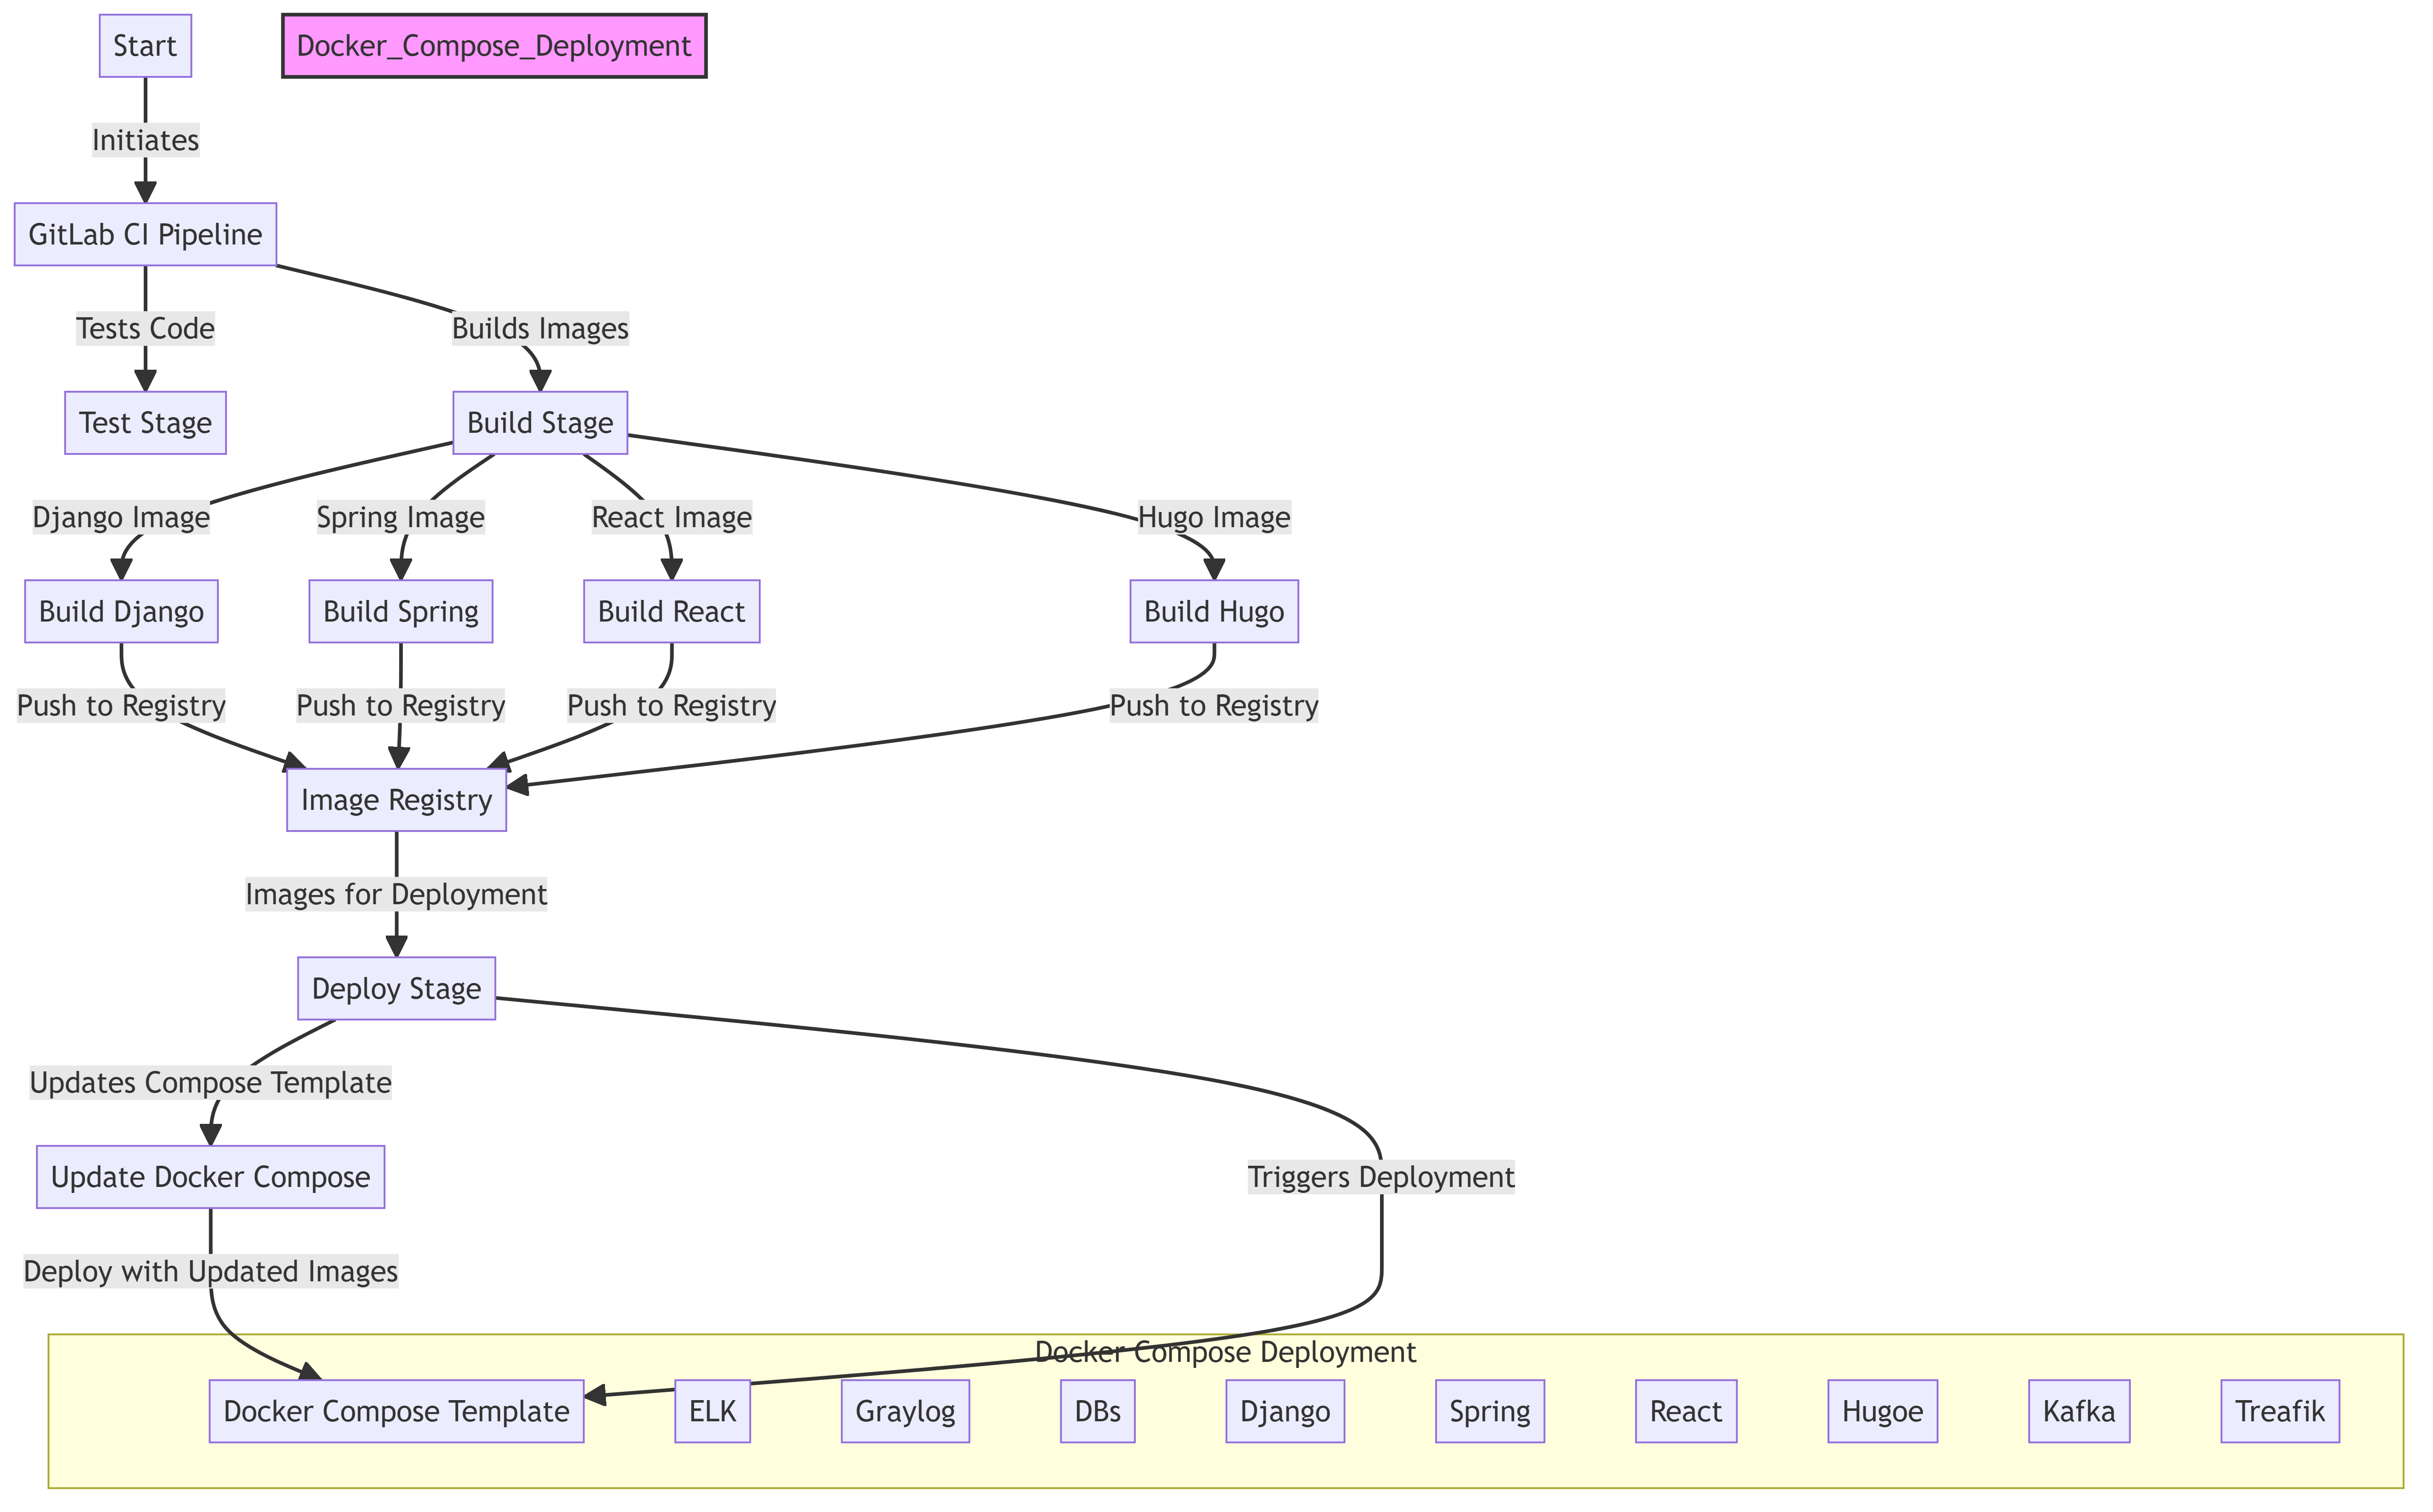
\includegraphics[width=1\textwidth,height=\textheight,keepaspectratio]{includes/figures/docker_deployment.png}
    \caption{Visuelle Darstellung des Deployment Prozesses in GitLab CI/CD und lokaler Umgebung}
    \label{fig:deployment_process}
\end{figure}


Der Prozess ist in der Datei \textit{.gitlab-ci.yml} hinterlegt und kann dort angepasst werden.
Wie in Abbildung \ref{fig:gitlab_ci_pipeline} zu sehen ist, werden die einzelnen Schritte als Jobs definiert und können auch einzeln ausgeführt werden.
Aktuell ist der Deployment Prozess nur für den Master Branch konfiguriert. Hier kann die eigene Vorgehensweise später gewählt werden.
Da aber im aktuellen Prozess nur vom Master abgezweigt wird und dieser immer im Produktivmodus zu laufen hat, gab es keine Notwendigkeit auf eine Git Flow basierte Branching Strategie zu wechseln. 
Dies wäre aber auch möglich, da die GitLab CI/CD Konfiguration auch auf Branches angewendet werden kann.




\begin{figure}[ht]
    \centering
    \begin{minipage}{0.5\textwidth}
        \centering
        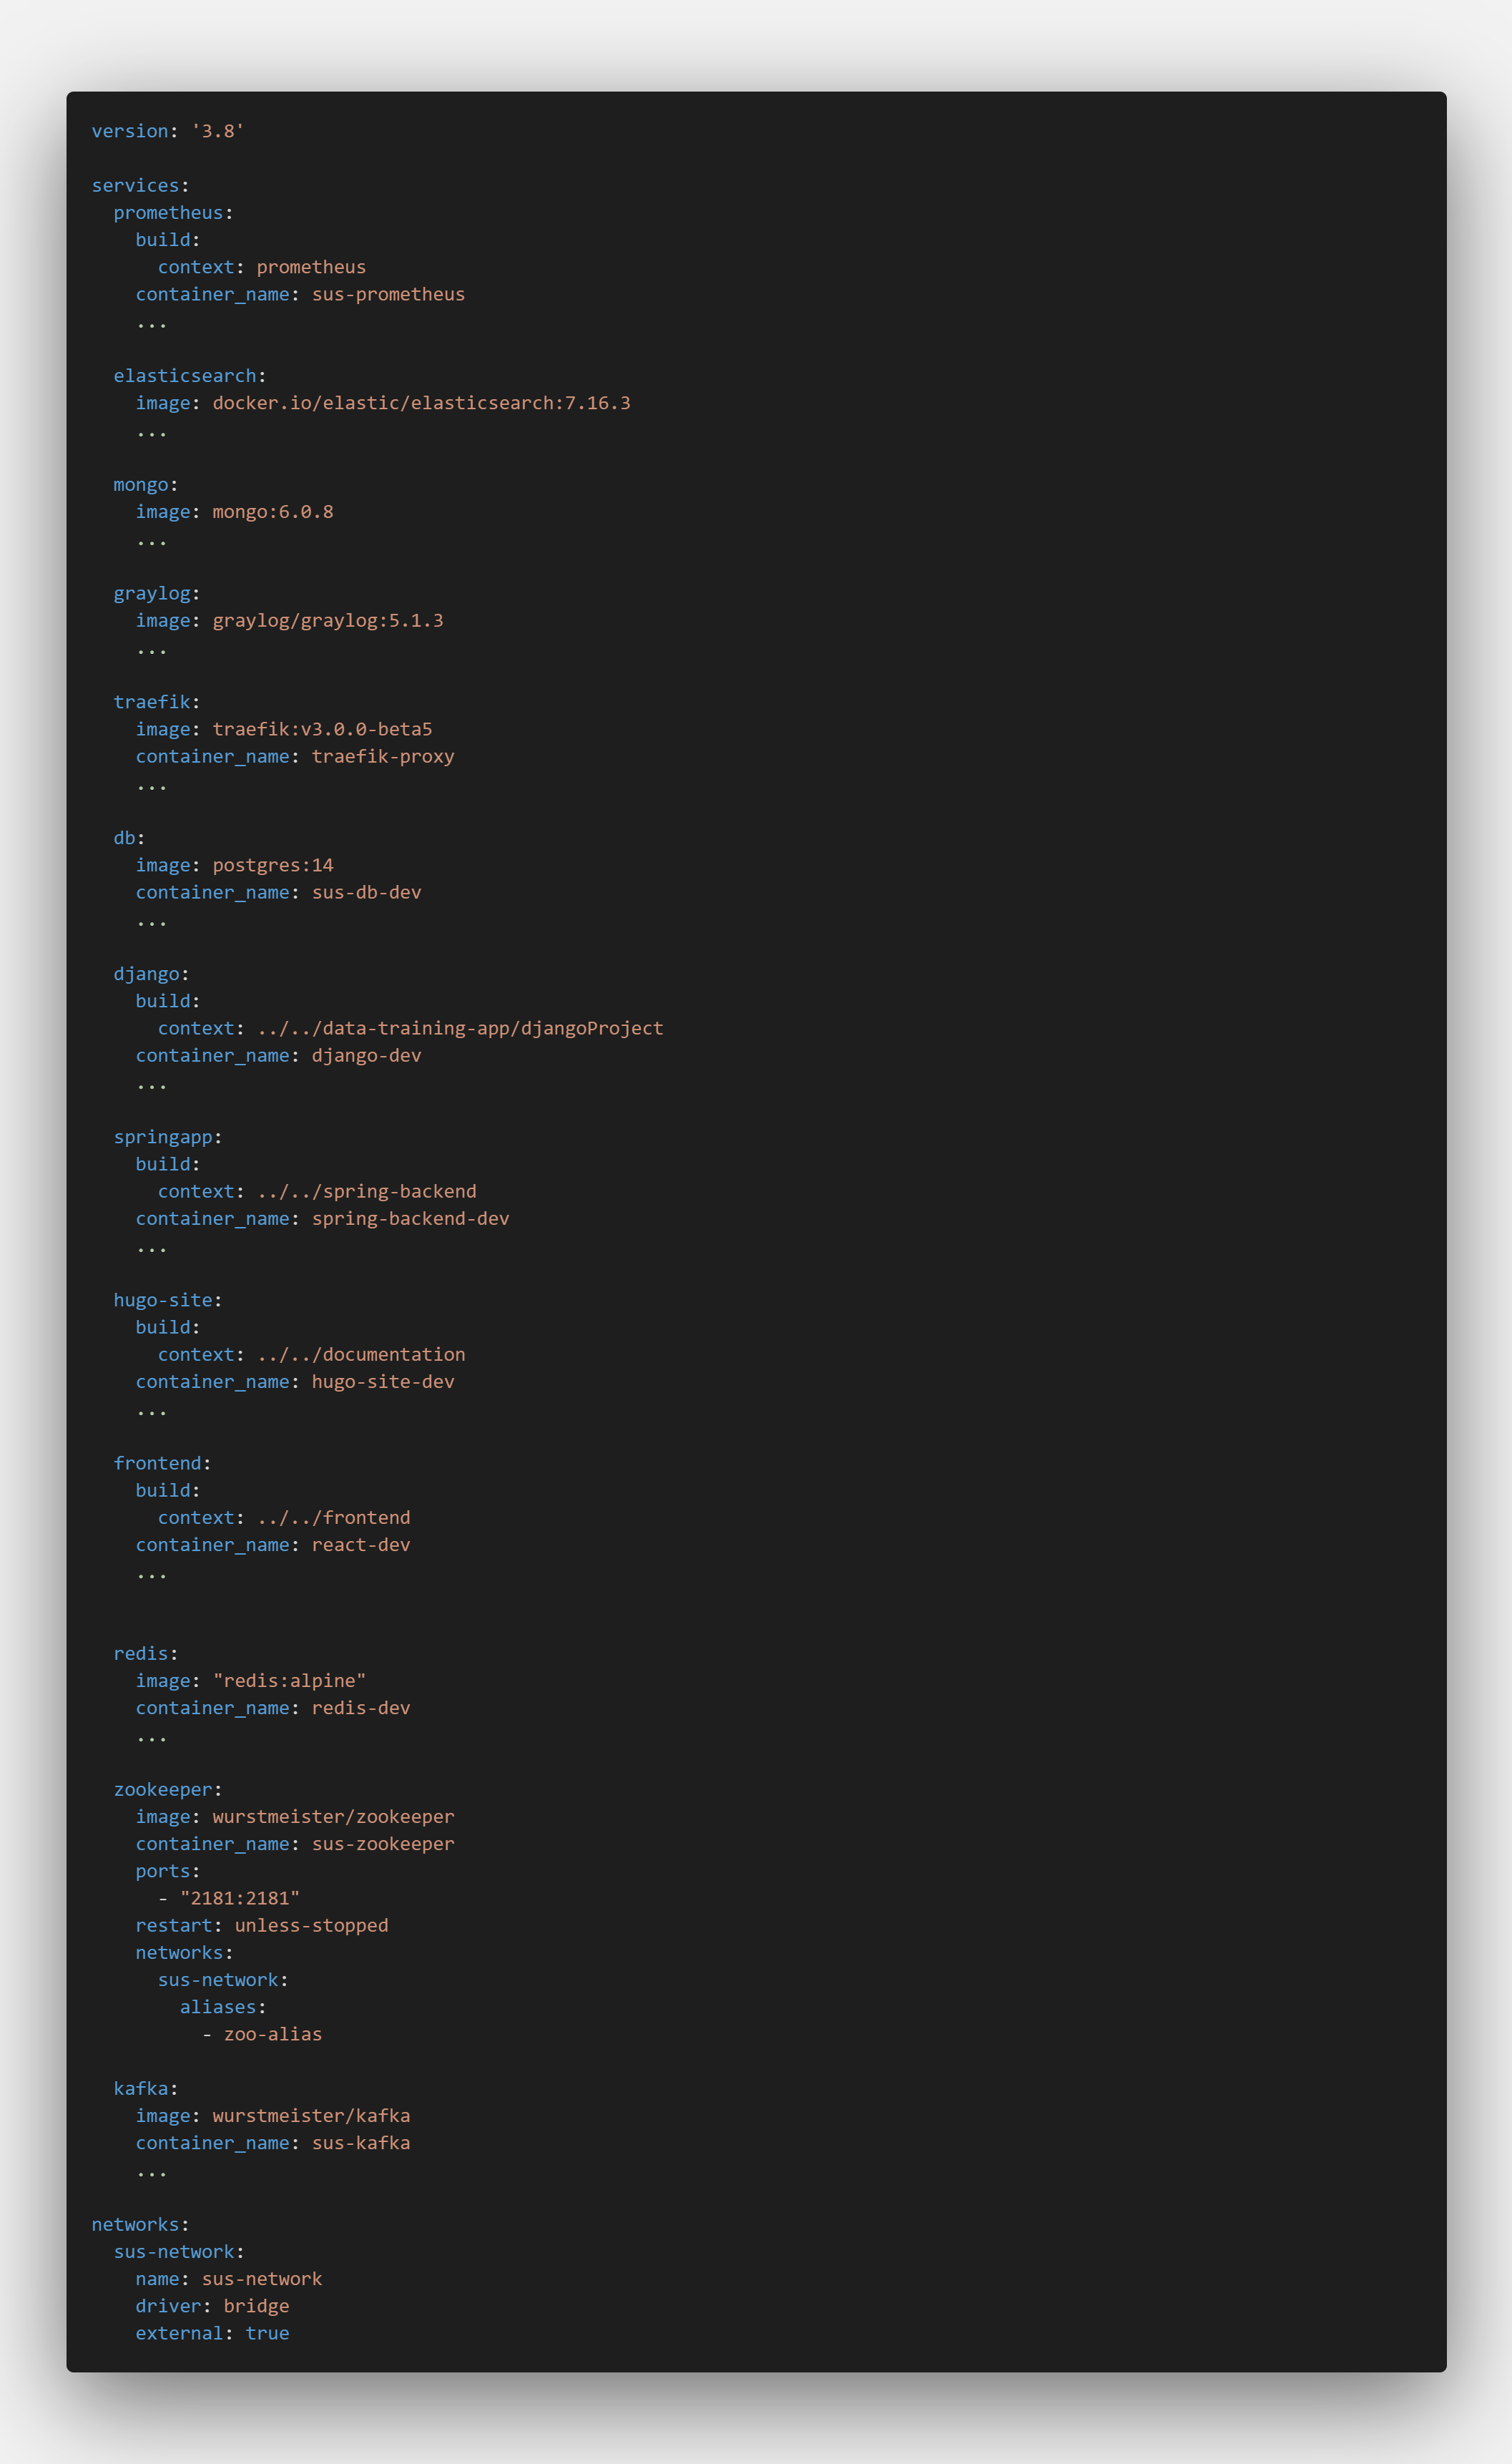
\includegraphics[width=\textwidth,height=\textheight,keepaspectratio]{includes/figures/code/code.png}
        \caption{Docker Compose File für den Produktionsprozess}
        \label{fig:code}
    \end{minipage}\hfill
    \begin{minipage}{0.5\textwidth}
        \centering
        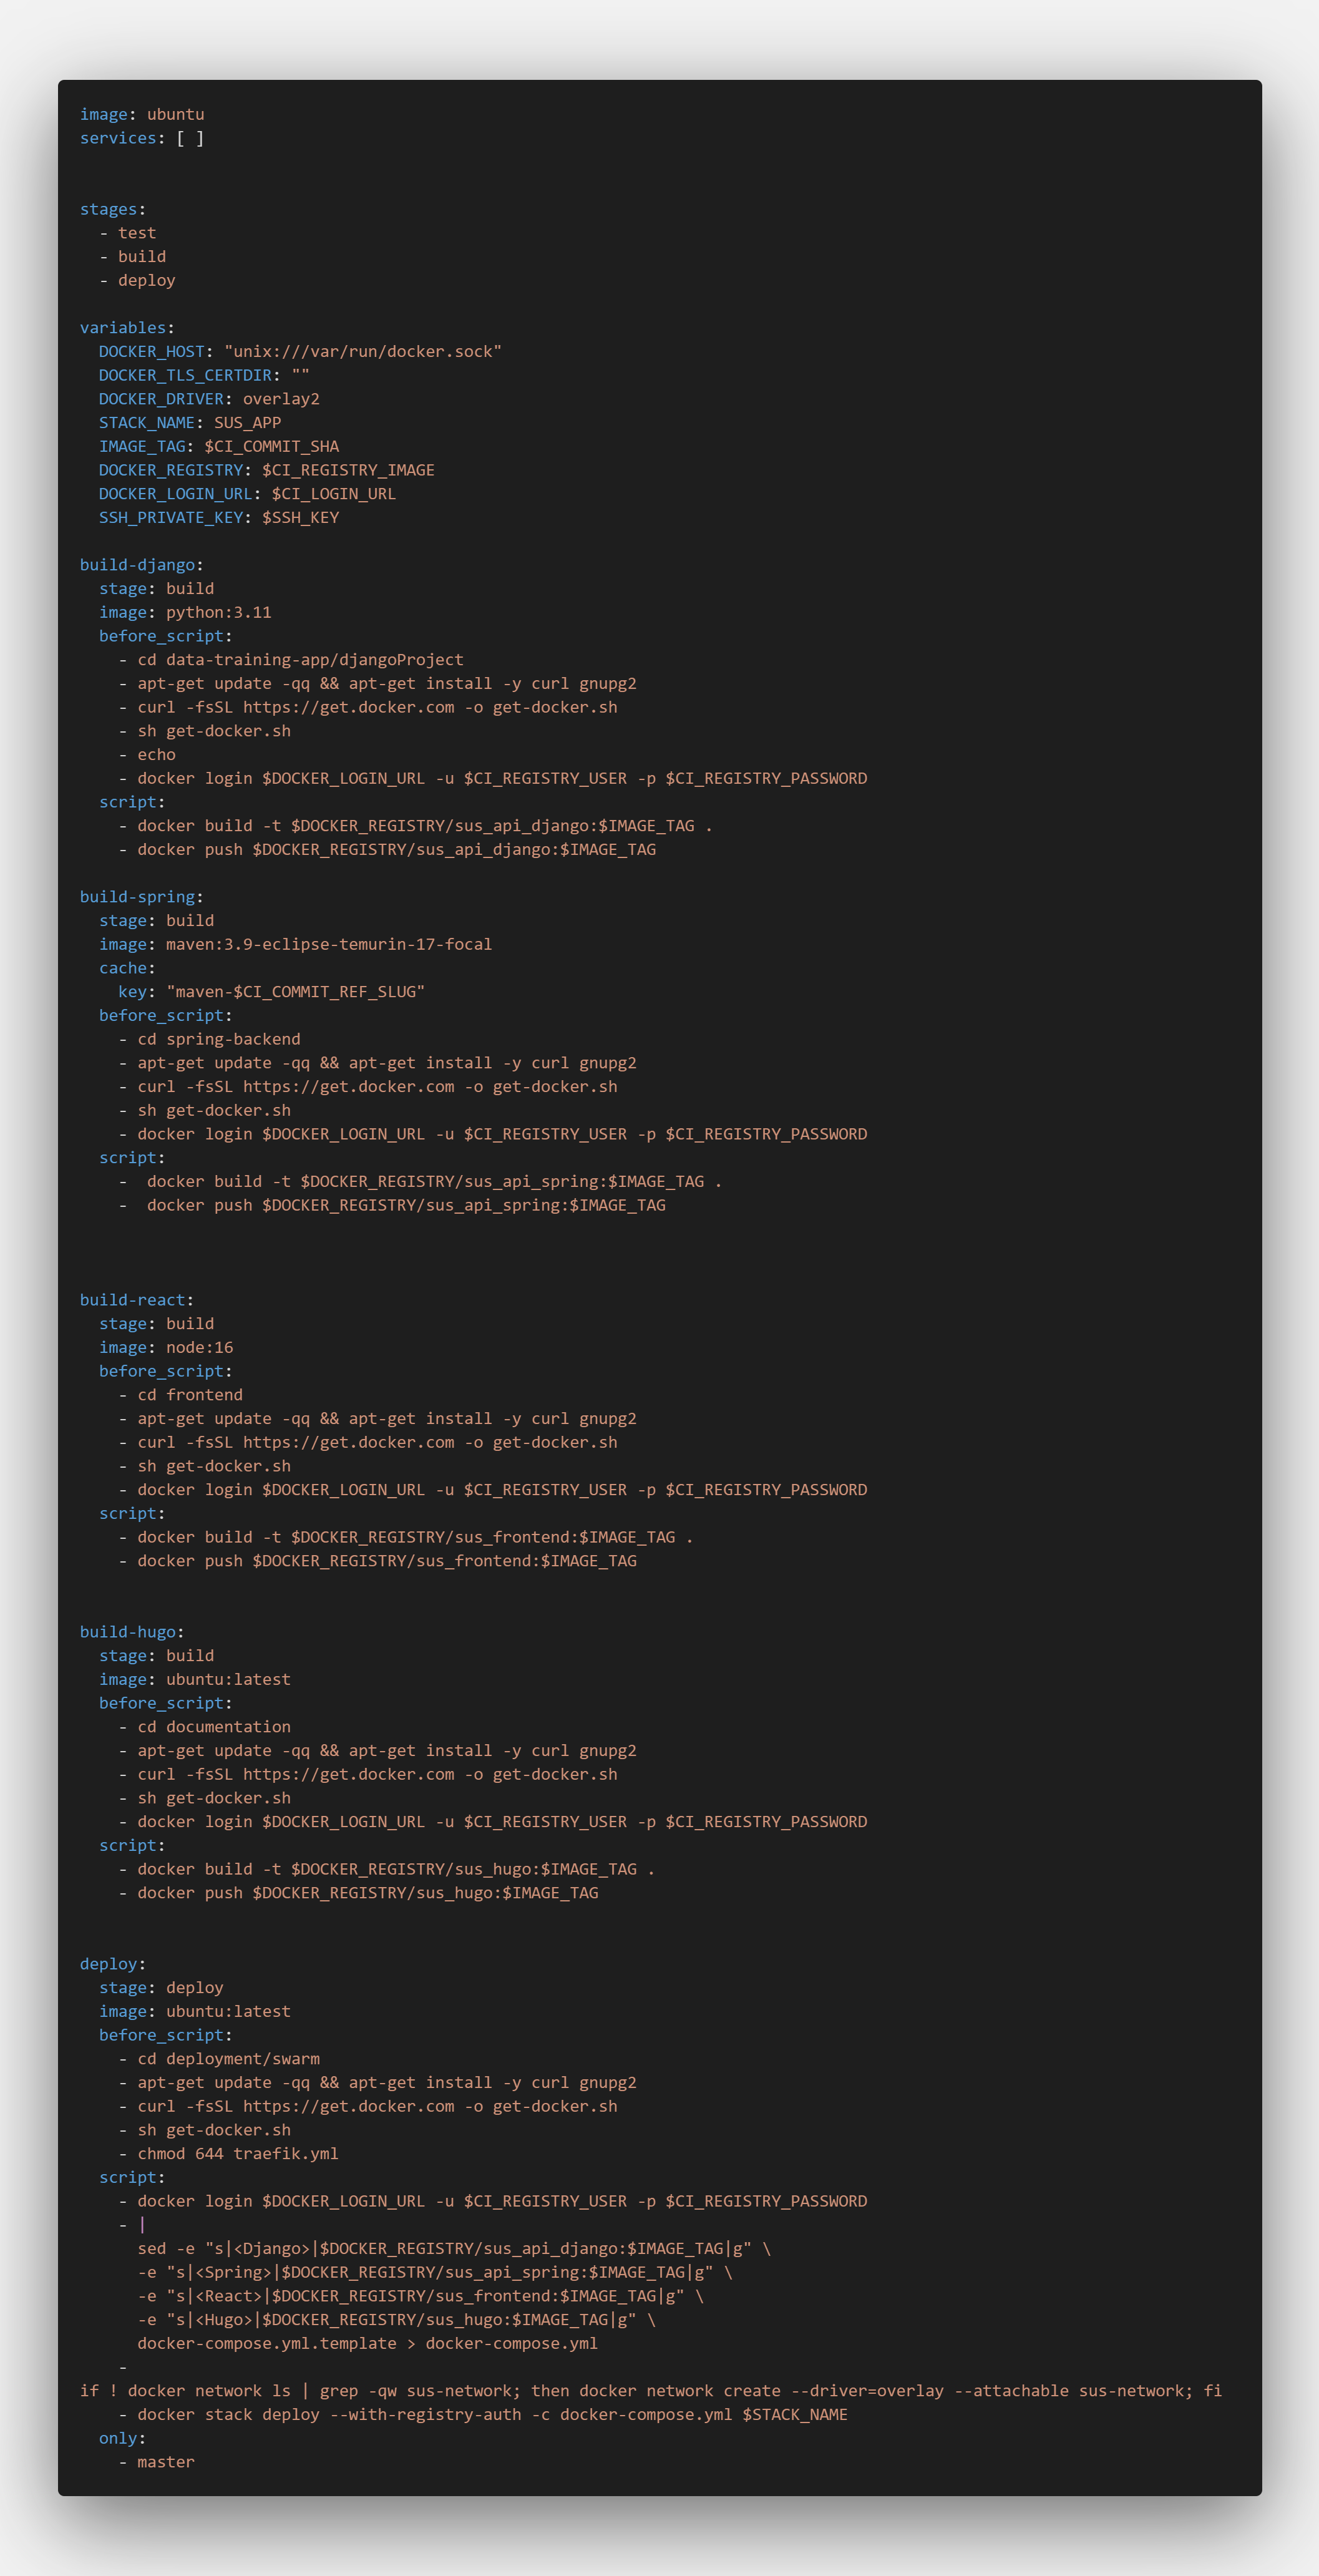
\includegraphics[width=\textwidth,height=\textheight,keepaspectratio]{includes/figures/code/gitlab_ci.png}
        \caption{Gitlab CI/CD Pipeline}
        \label{fig:gitlab_ci_pipeline}
    \end{minipage}
\end{figure}

% !TeX program = xelatex

\chapter{Ereignisse und Auswertung der Modelle und Algorithmen}
\label{cha:events_and_evaluation}

\section{Trainingsdaten}
Die Bewertung der einzelnen Metriken ist nicht trivial, da die synthetischen Daten nicht nur ähnlich, sondern nicht identisch zu den realen Daten sein sollen. Während bei den meisten Metriken hauptsächlich auf die Übereinstimmung der Daten geschaut wird, oder wie stark deren Verteilungen übereinstimmen, so ist dieser Wert wenig aussagekräftig.
Abweichungen, Werte die nicht in die normale Verteilung passen und andere Abweichungen sind gewollt und dürfen nicht als schlecht bewertet werden.
Visuell lässt sich leicht ein Unterschied zwischen den Daten erkennen, auch kann eingeschätzt werden in wie weit die Daten dem gleichen Muster folgen (siehe Abbildung \ref{fig:real_vs_synth}), nur ist dies kein klassifizierbares Maß.



\begin{figure}[ht]
    \centering
    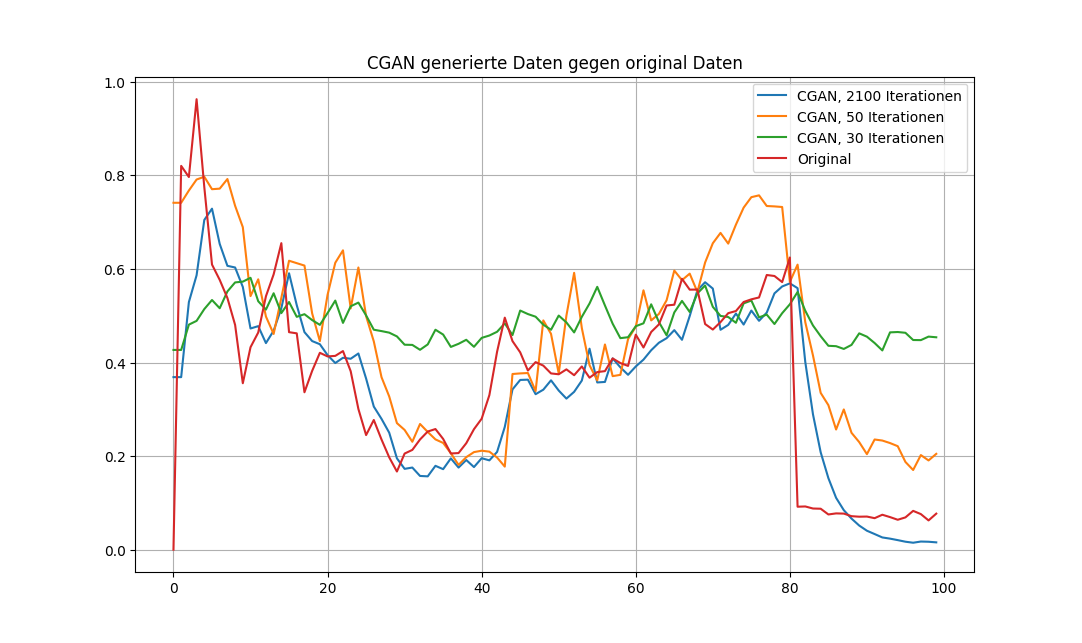
\includegraphics[width=0.8\textwidth]{includes/figures/real_vs_synth.png}
    \caption{Vergleich von realen und synthetischen Daten}
    \label{fig:real_vs_synth}
\end{figure}


\begin{table}[ht]
    \centering
    \caption{Autokorrelation der Datensätze}
    \begin{tabular}{ll}
        \toprule
        \textbf{Dataset Name}   & \textbf{Auto-correlation Coefficient} \\
        \midrule
        weather\_normalized     & 0.7531247393640502                    \\
        stockdata\_normalized   & 0.8705377400789976                    \\
        electricity\_normalized & 0.9213733429685765                    \\
        corona\_normalized      & 0.9705517108865852                    \\
        sinus                   & 0.992051245850721                     \\
        \bottomrule
    \end{tabular}
    \label{tab:autocorrelation_coefficients}
\end{table}


Um die Modelle und Algorithmen später vernünftig zu testen und vergleichen zu können, wurden sie mit 5 verschiedenen Trainingsdaten trainiert.
Diese besitzen jeweils unterschiedliche Komplexität, welche hier durch ihre Autokorrelationswerte angeben und in Tabelle \ref{tab:autocorrelation_coefficients} zu finden ist, und sollen so die Stärken und Schwächen der einzelnen Algorithmen aufzeigen.
Die wohl am einfachten zu erlernenden Daten sind Sinus Kurven. Diese sind leicht zu erlernen und können mit wenigen Parametern beschrieben werden.
In Abbildung \ref{fig:sinus_data} sind die Daten zu sehen.

\begin{figure}[ht]
    \centering
    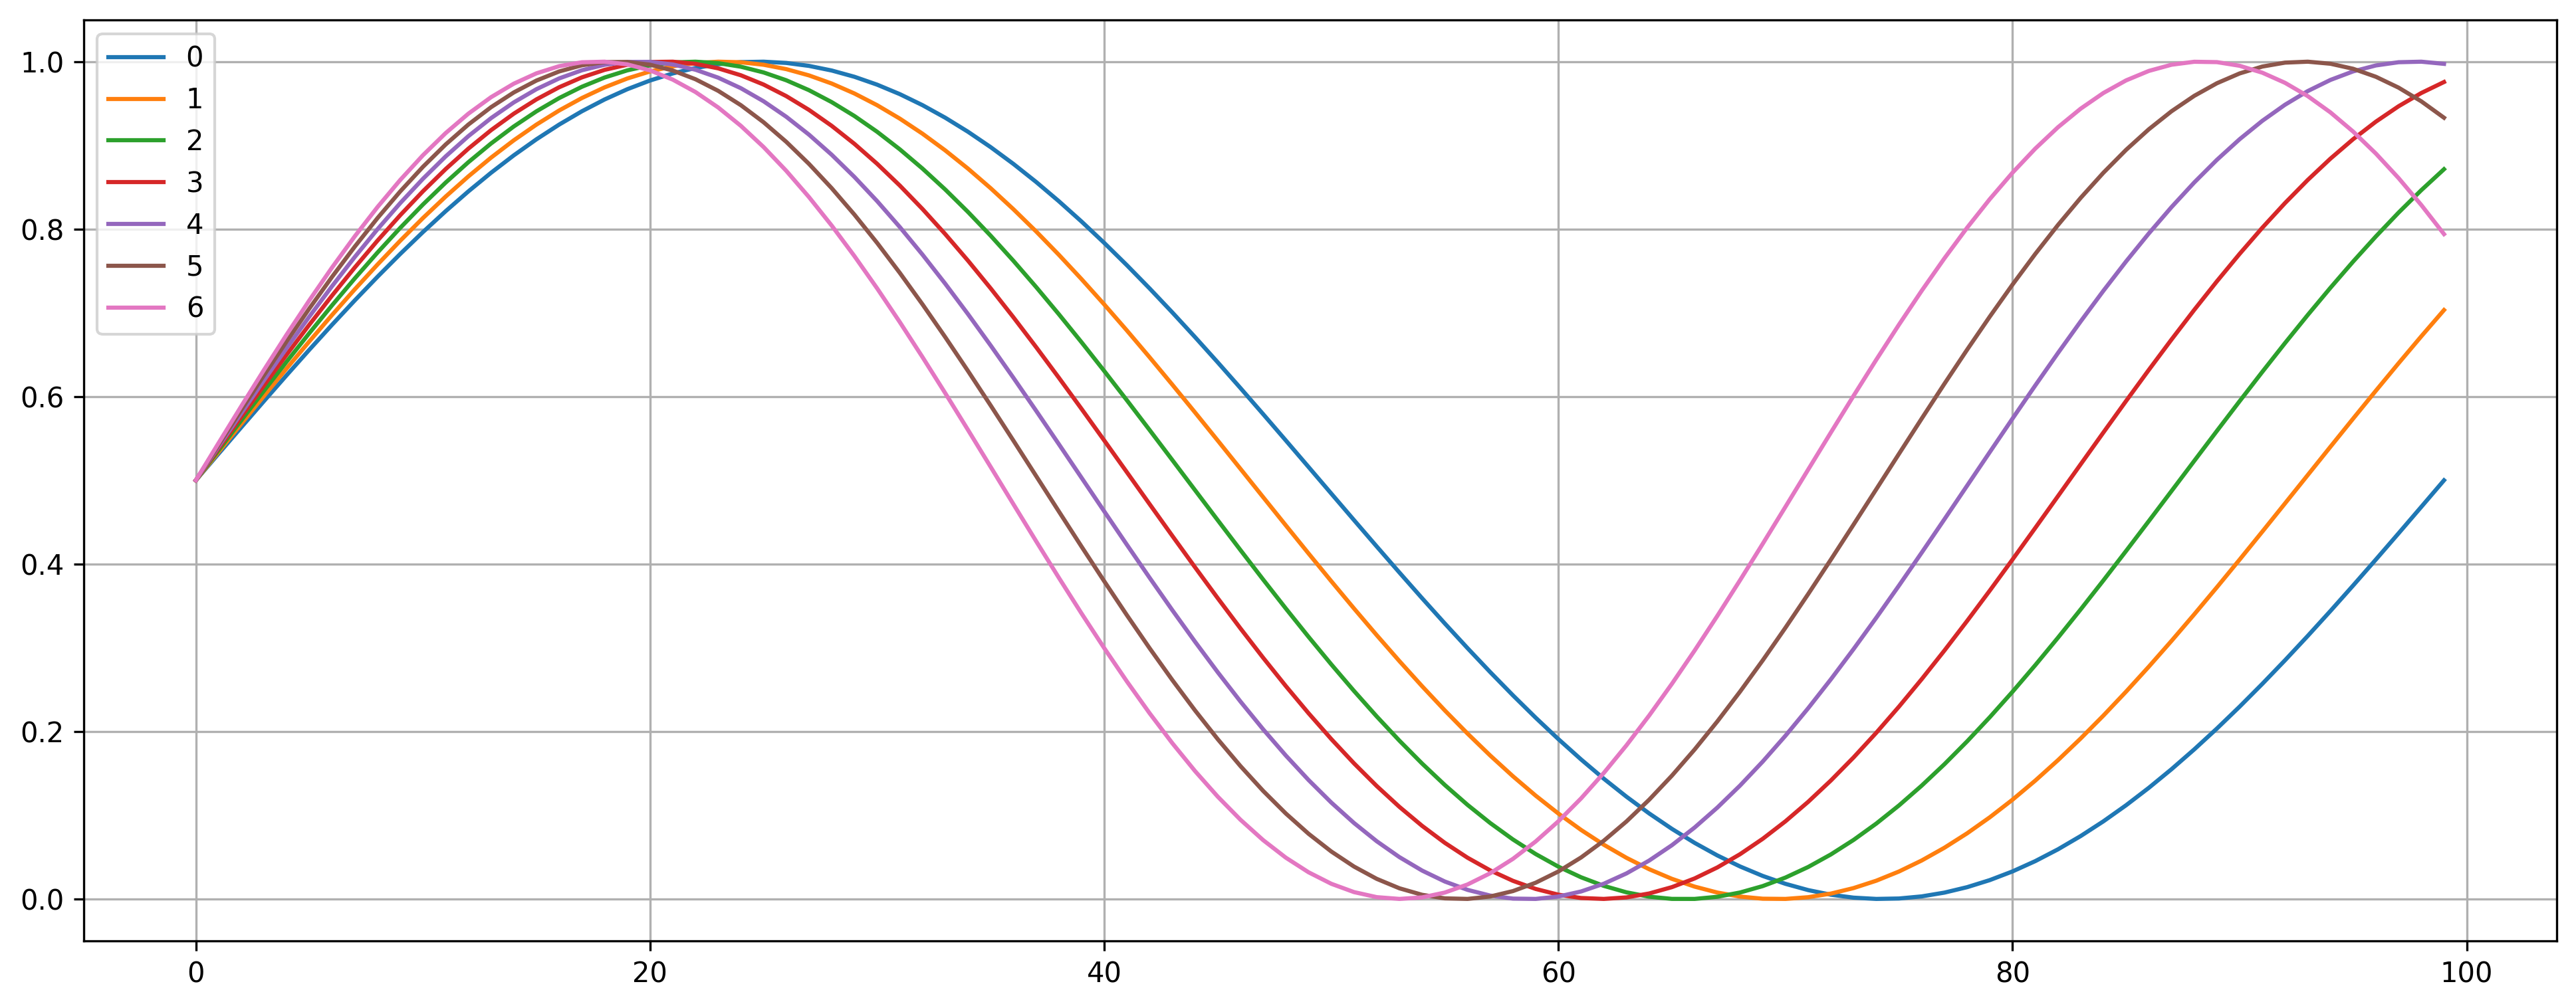
\includegraphics[width=1\textwidth]{includes/figures/graphs/sinus.png}
    \caption{Sinus Kurven als Testdaten}
    \label{fig:sinus_data}
\end{figure}

Die genutzten Corona Daten zeigen den Anstieg zum Beginn der Pandemie, und sind daher wenig komplex. Diese stammen von \cite{covid19g12:online} und sind in Abbildung \ref{fig:covid_data} zu sehen.

\begin{figure}[ht]
    \centering
    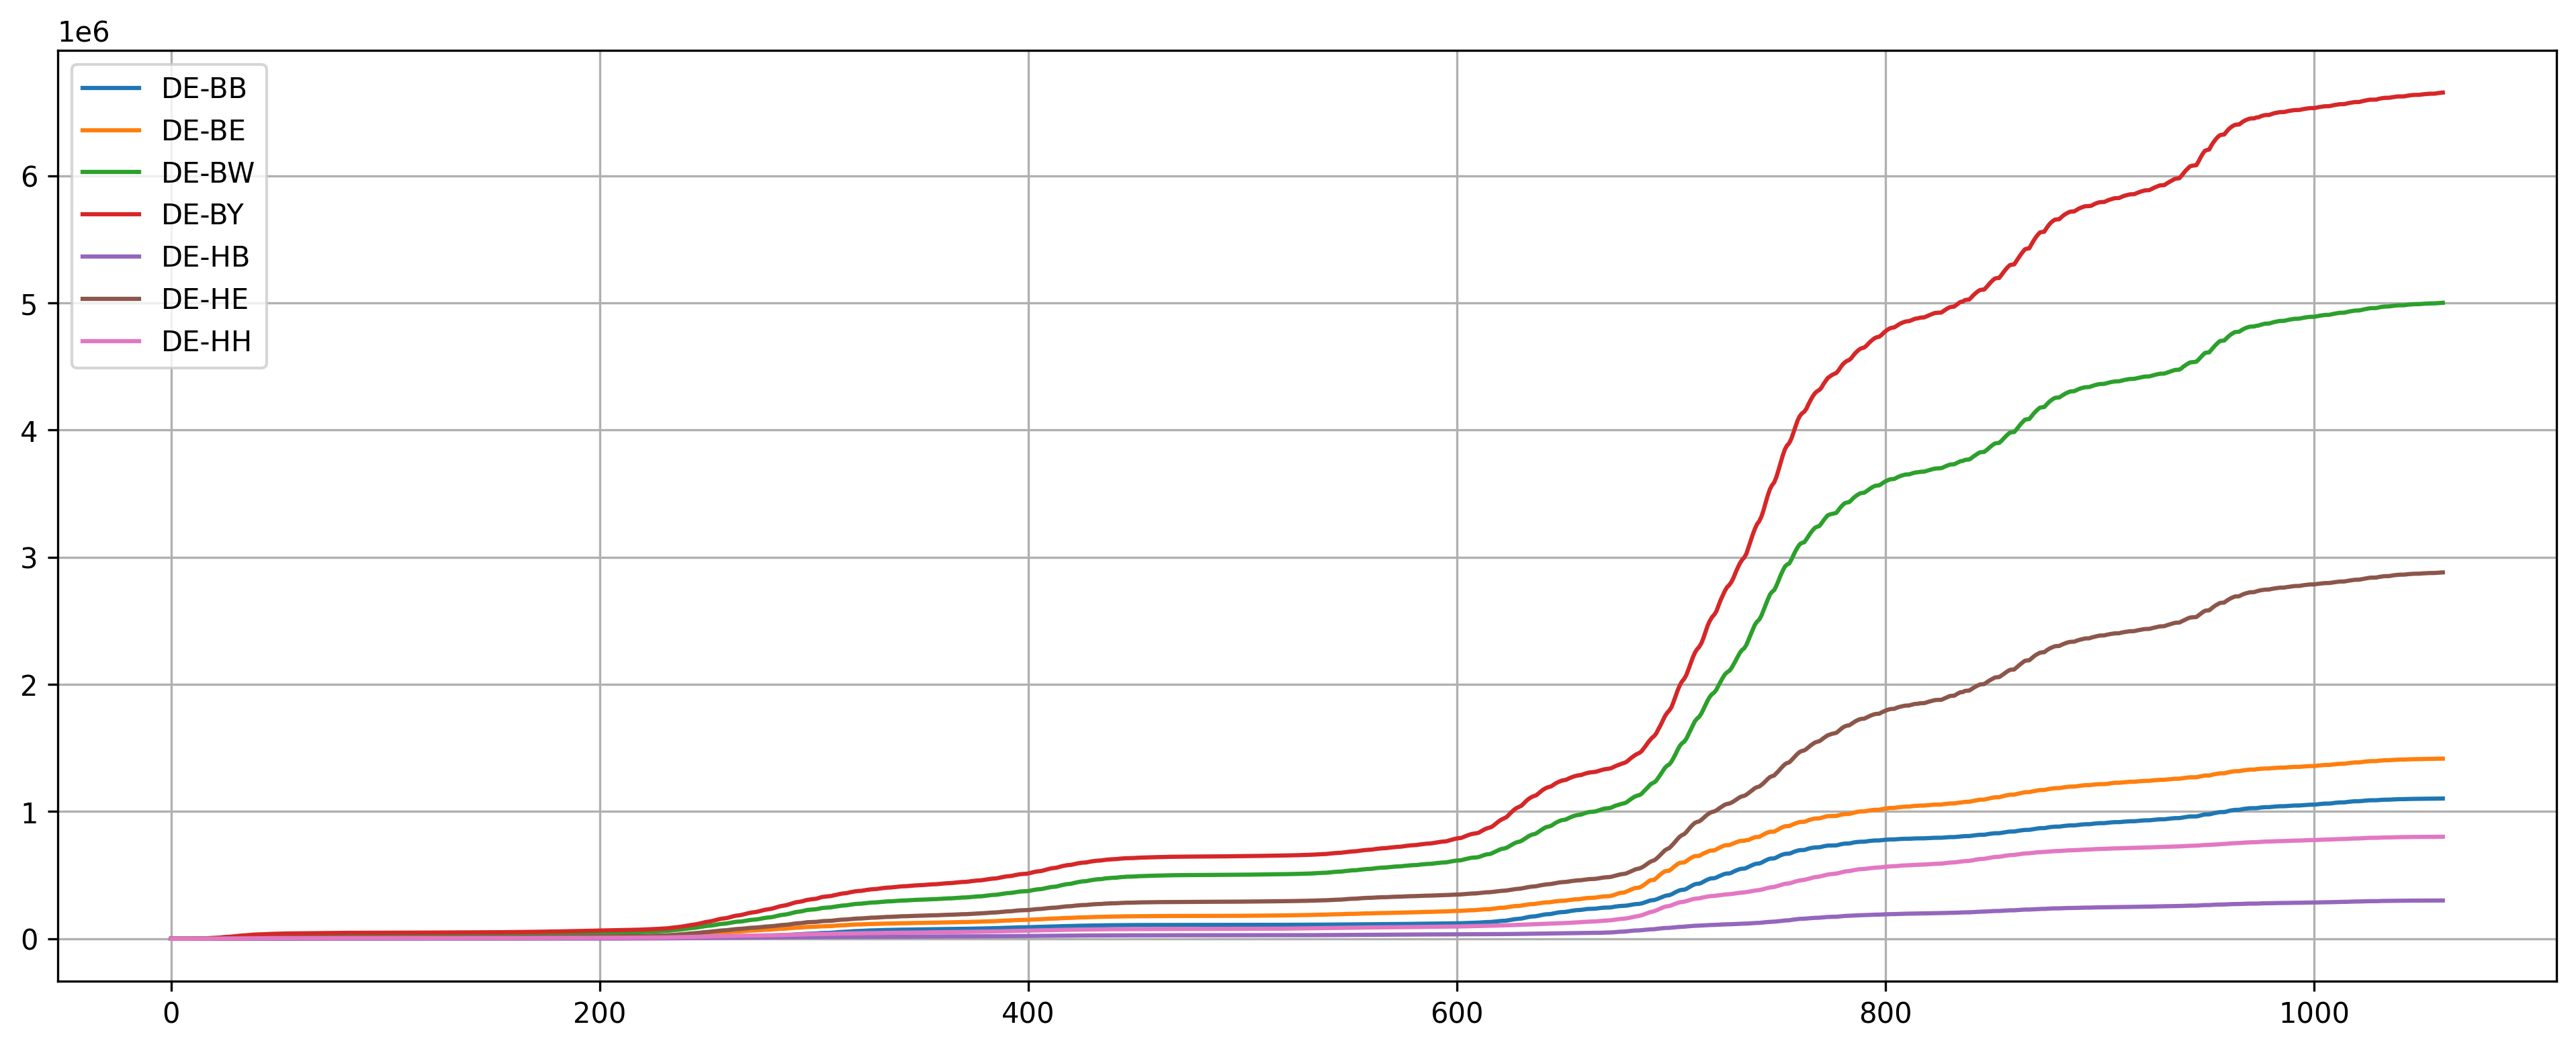
\includegraphics[width=1\textwidth]{includes/figures/graphs/corona_test_cases.png}
    \caption{Infektionszahlen einiger Bundesländer zu Beginn der Pandemie als Testdaten}
    \label{fig:corona_data}
\end{figure}

Etwas komplexer sind die Daten über den Stromverbrauch von unterschiedlichen Verbrauchern über mehrere Tage hinweg, der genutzte Datensatz misst die Werte für verschiedenen Haushalte über etwas mehr als 30 Tage im stündlichen Takt. Sie stammen von \cite{longterm99:online} und hatten leider wenige Information über die Art der Daten.
Hier treten periodische Muster auf, welche aber nicht so einfach zu erlernen sind wie die Sinus Kurven und damit eine größere Herausforderung darstellen.
Auch sind hier Außreißer und andere Abweichungen von der Norm zu erwarten. Die Daten sind in Abbildung \ref{fig:electric_data} zu sehen.

\begin{figure}[ht]
    \centering
    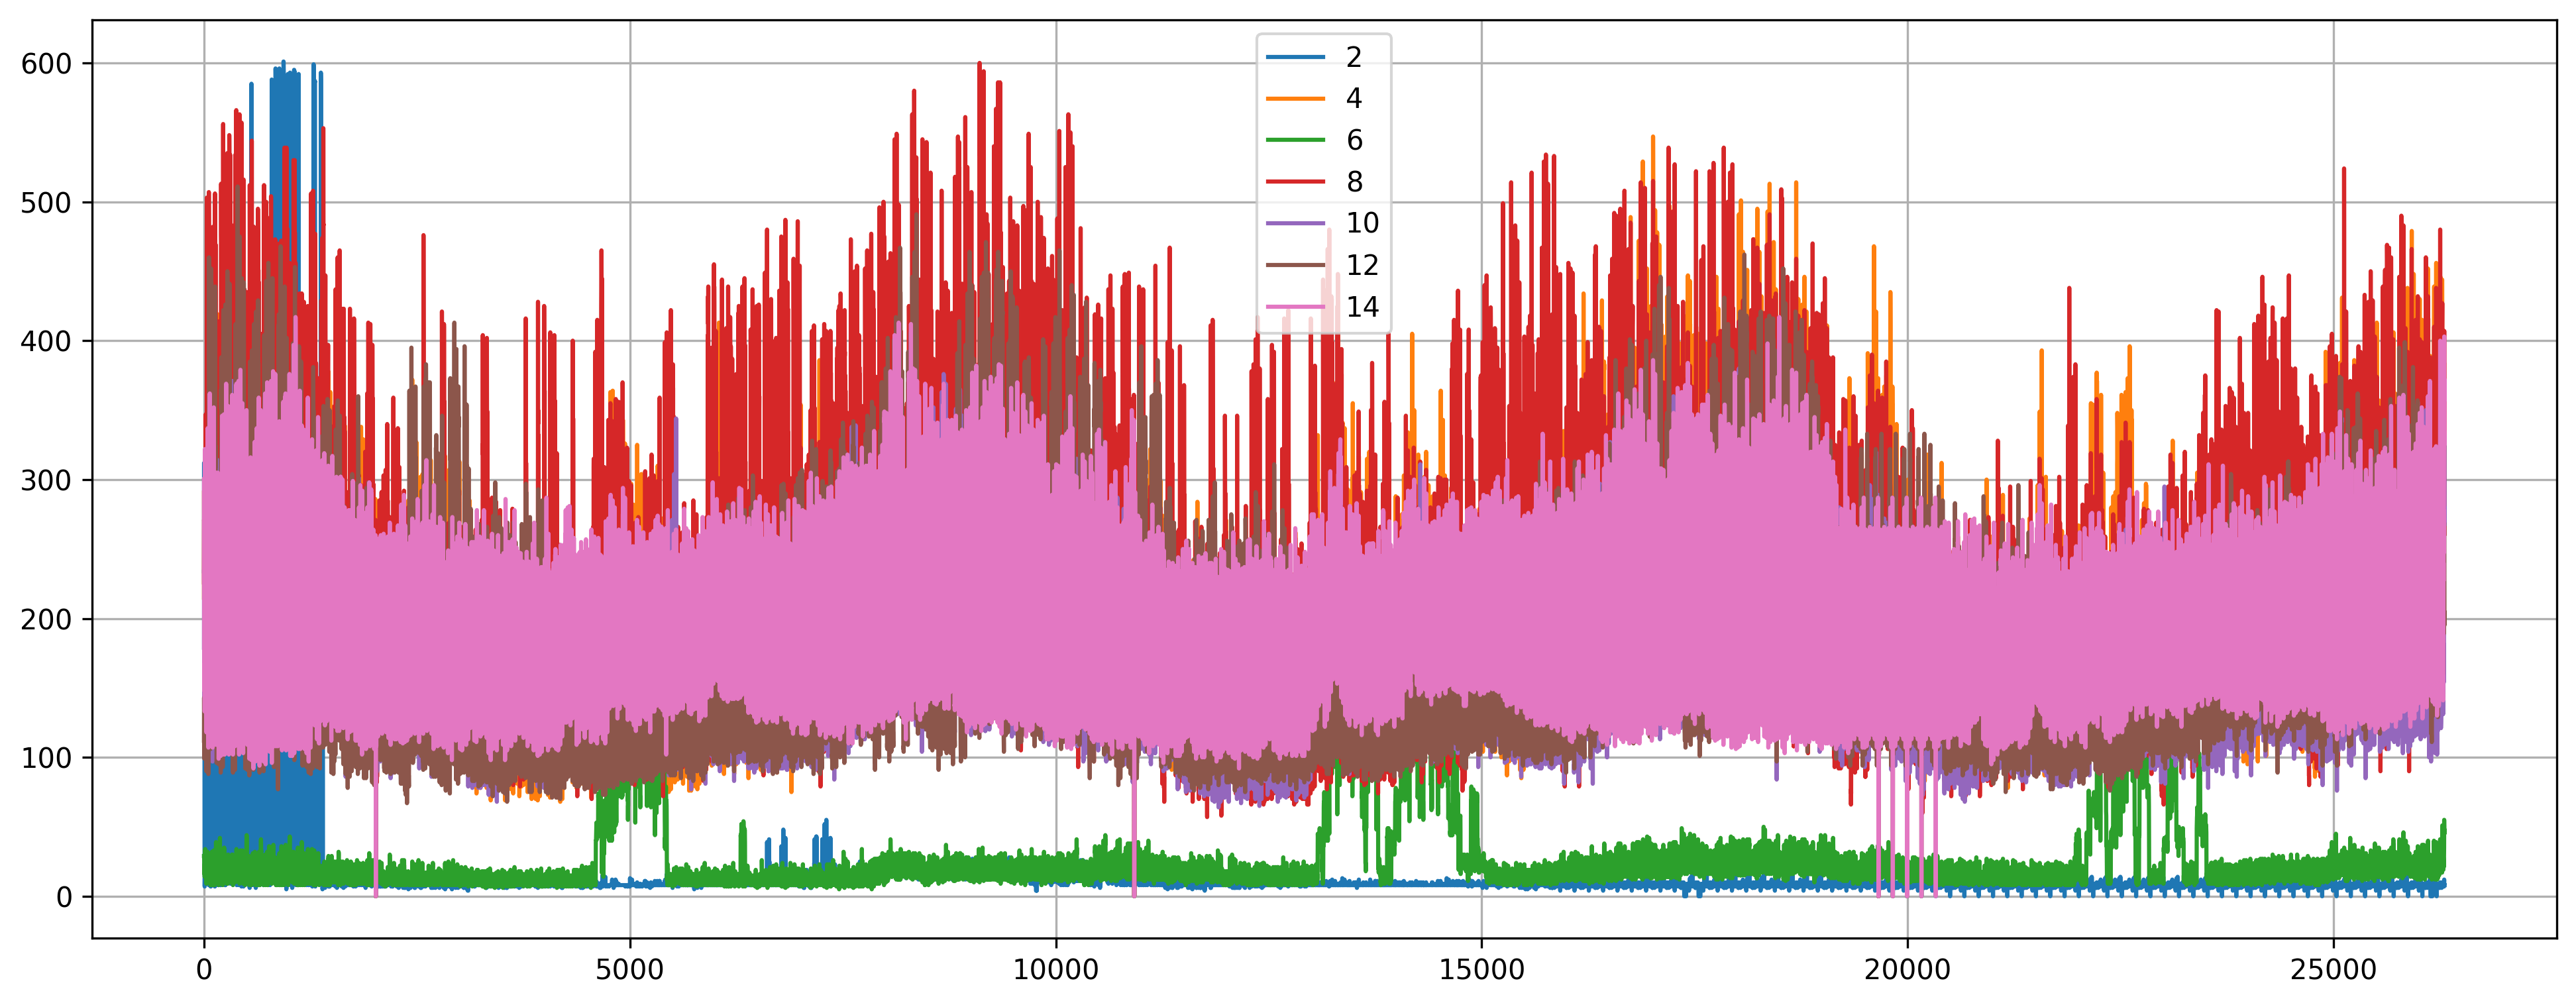
\includegraphics[width=1\textwidth]{includes/figures/graphs/electricity.png}
    \caption{Elektrizitätsverbrauch als Testdaten}
    \label{fig:electric_data}
\end{figure}



Sehr interessant sind auch Aktiendaten. Diese sind sehr komplex, nicht zwangsläufig periodisch und besitzen viele Abweichungen von der Norm. Sie sind deutlich komplexer zu erlernen, da sie keinen direktem Muster folgen.
Die Daten sind in Abbildung \ref{fig:stock_data} zu sehen und wurden über Yahoo Finanzen\footnote{https://de.finance.yahoo.com/} erworben. Da es sich um die selber Aktie und verschieden Werte handelt, wie beispielsweise deren höchsten, niedrigersten oder durschnittlichen Preis, sind die Daten sehr ähnlich, aber nicht identisch.

\begin{figure}[ht]
    \centering
    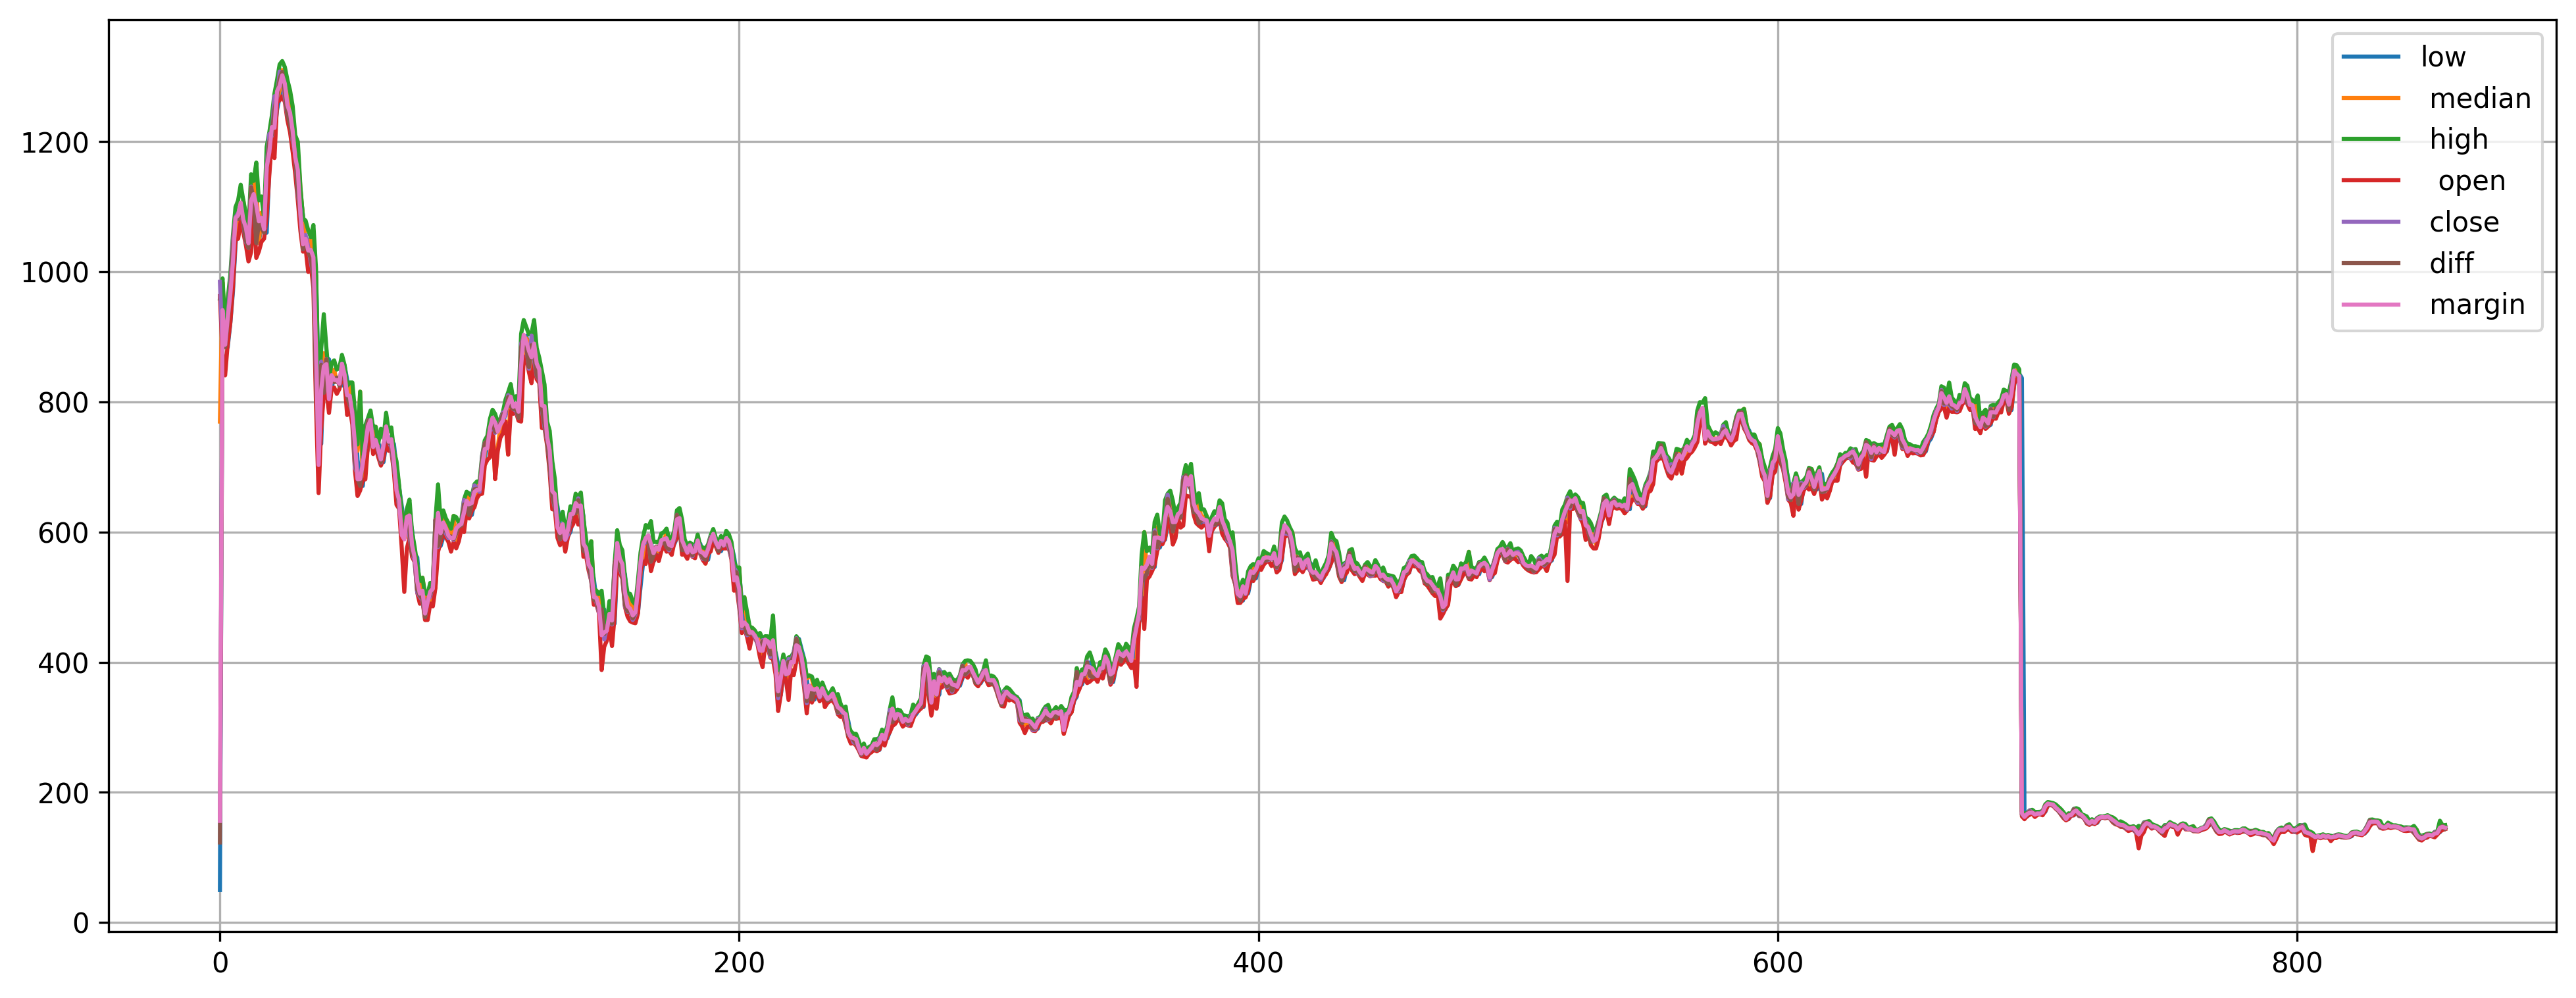
\includegraphics[width=1\textwidth]{includes/figures/graphs/stockdata.png}
    \caption{Aktiendaten als Testdaten}
    \label{fig:stock_data}
\end{figure}



Interesannter weise sind die Wetterdaten über einen gewissen Zeitraum am komplexesten. Diese sind Teilweise periodisch, aber auch nicht immer. 
Dazu kommt der Umstand, dass nicht nur Temperaturen, sondern auch Luftdruck und andere Werte mit aufgenommen wurden. Ein Überblick ist in Abbildung \ref{fig:weather_data} zu sehen. Sie stammen auch von \cite{longterm99:online} und es gibt daher 
auch keine weiteren Informationen über die Daten.

\begin{figure}[ht]
    \centering
    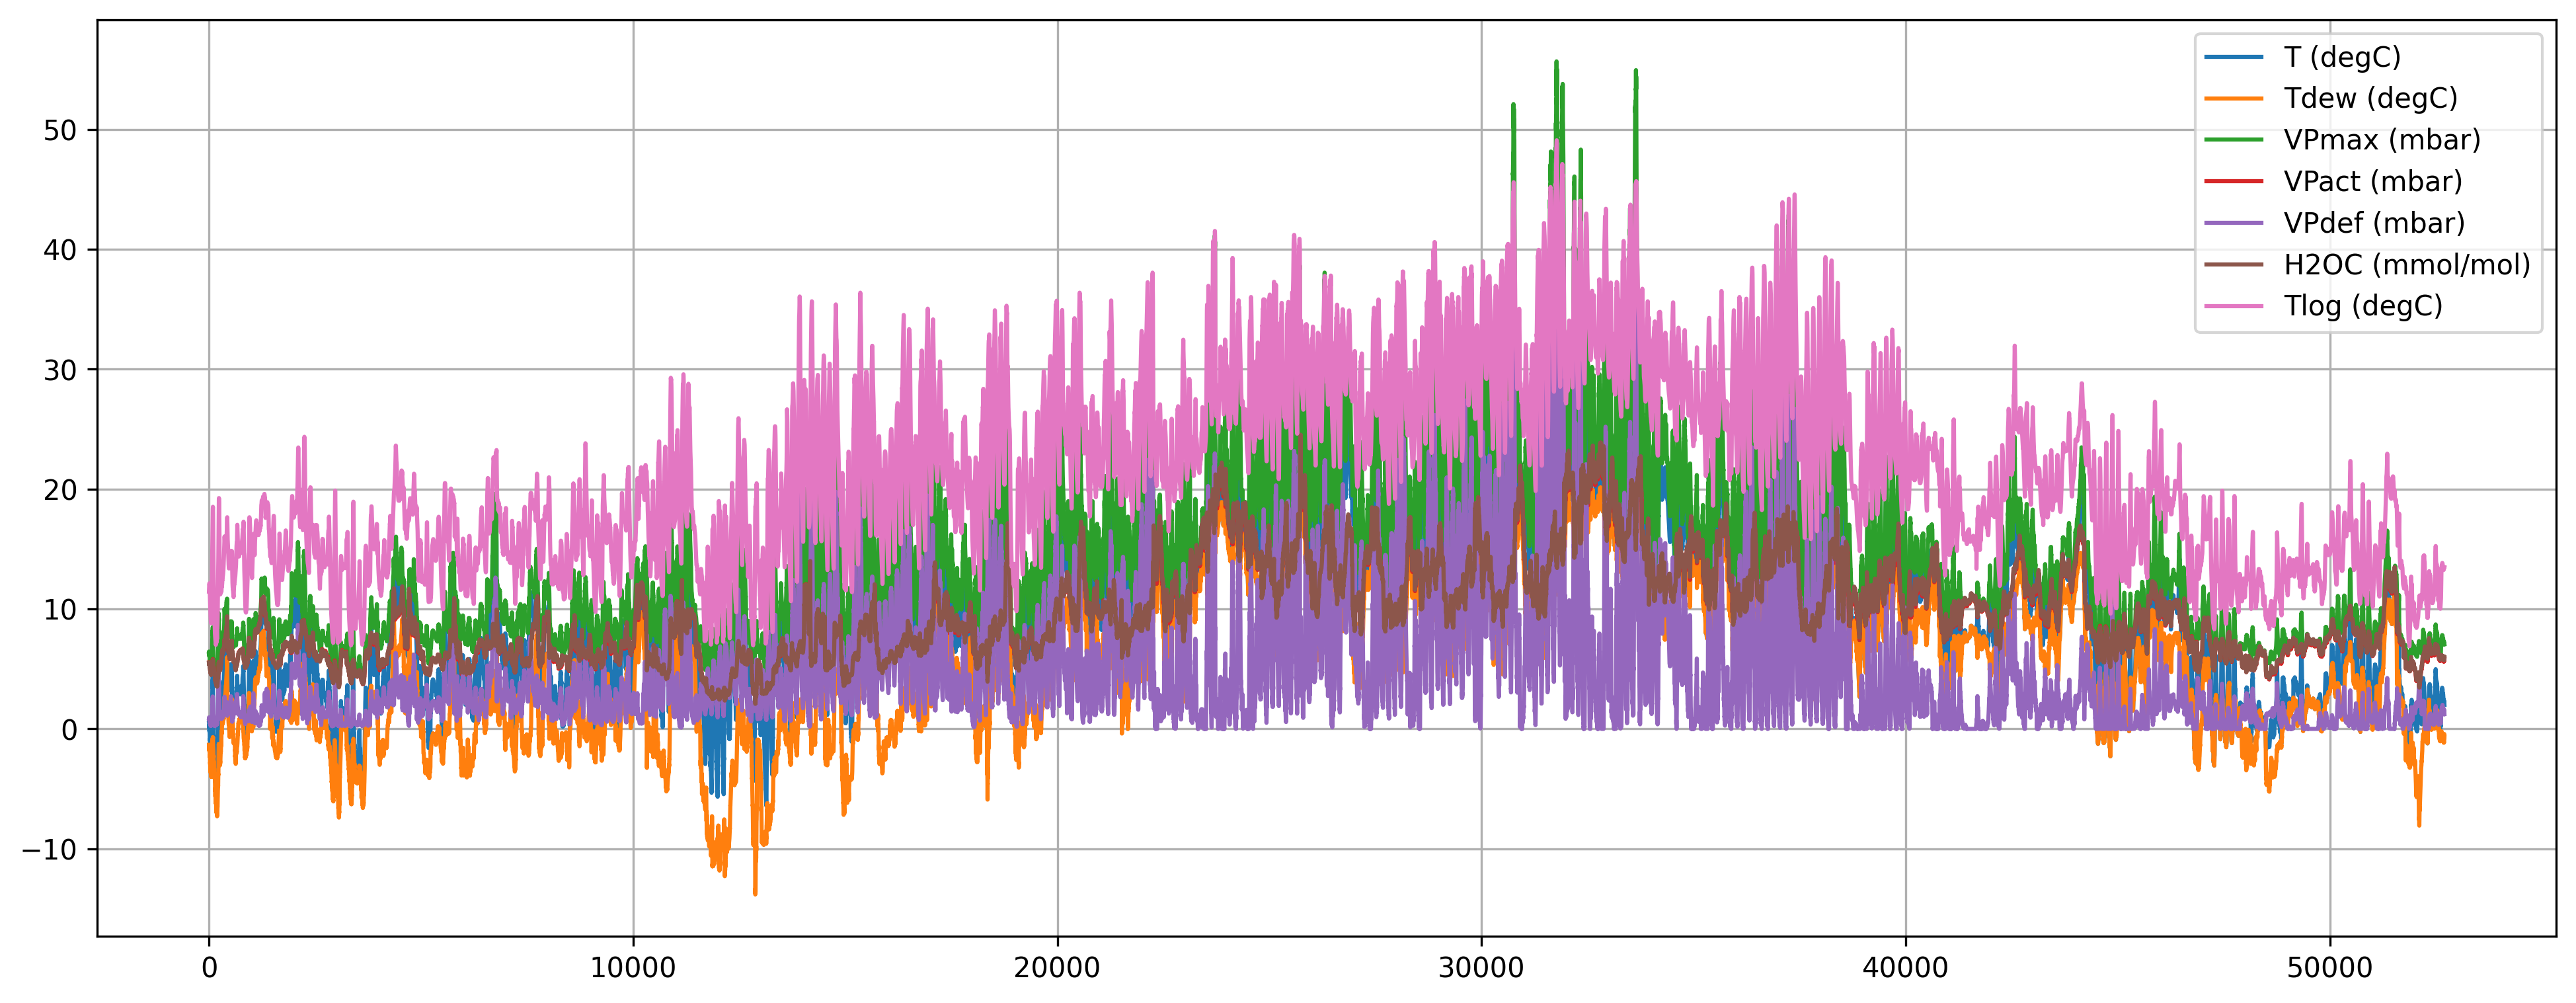
\includegraphics[width=1\textwidth]{includes/figures/graphs/weather.png}
    \caption{Wetterdaten als Testdaten}
    \label{fig:weather_data}
\end{figure}


\section{Vergleich der Algorithmen und Modelle}

\subsection{Performance Metriken der ML Modelle}

Um die Vergleichbarkeit der einzelnen Metriken zu gewährleisten, wurden die realen Daten alle ersteinmal uniformiert. Dies bedeutet, dass die Daten auf einen Wertebereich von 0 bis 1 skaliert wurden und auf die gleiche Anzahl an Elementen je Zeitreihe gebracht wurden.
Somit lässt dich der Vorverarbeitungsschritt entfernen und die Modelle können direkt auf den Daten trainieren.

Grundsätzlich sind die Trainingszeiten der generativen Modelle stark unterschiedlich. Modelle aus der tsgm Bibliothek \cite{nikitin2023tsgm} sind deutlich deutlich langsamer als die nativen keras Modelle, welche selber implementiert wurden.
Da aber die tsgm Modelle bei weitem komplexer sind und bereits nutzbare Ergebnisse mit wenigeren Iterationen liefern, wurde hier die Zahl der Iterationen reduziert, um die Laufzeit zu verkürzen.
Der Test wurde nur mit wenigen Iterationen durchgeführt, da hier am entscheidensten die Menge an Daten zum Training relevant war.
Um die Einflüsse anderer Programme auf dem System zu eliminieren oder wenigstens zu minimieren wurde der Test in einen eigens hierfür erstellten Docker Containern durchgeführt. Dieser Container wurde mit 2 \ac{CPU} Kernen und 8 \ac{GB} \ac{RAM} ausgestattet.

\begin{figure}[ht]
    \centering
    \begin{minipage}{0.6\textwidth}
        \centering
        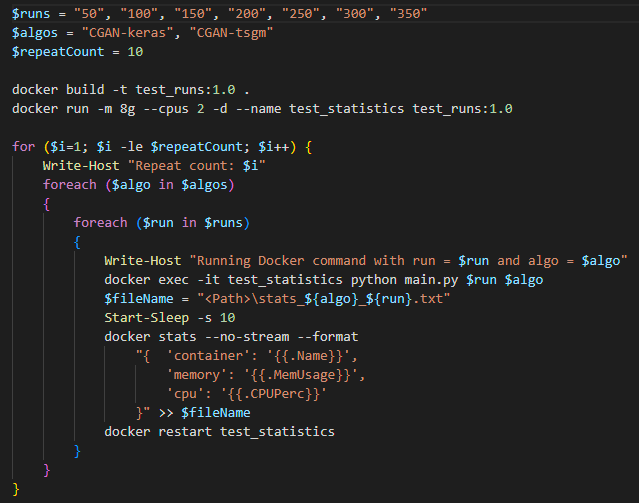
\includegraphics[width=\textwidth]{includes/figures/code/powershell_for_testing.png}
        \caption{PowerShell Script zum Testen der Modelle in einem Docker Container}
        \label{fig:test_run_powershell}
    \end{minipage}\hfill
    \begin{minipage}{0.38\textwidth}
        \centering
        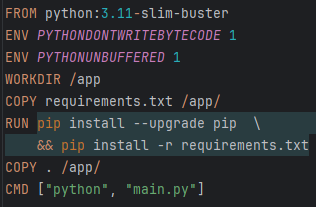
\includegraphics[width=\textwidth]{includes/figures/code/Dockerfile_for_testing.png}
        \caption{Dockerfile zum Erstellen des Docker Containers}
        \label{fig:test_run_dockerfile}
    \end{minipage}
\end{figure}

Da sowohl die tsgm Bibliothek als auch selber eine Implementierung der \ac{CGAN} Architektur erstellt wurde, bat es sich an diese als Vergleich zu nutzen. Wie in Abbildung \ref{fig:test_run_powershell} zu sehen ist, wird der Docker Container über ein Powershell Script gebaut, startet das Python Script, speichert alle notwendigen Metriken und startet den Container neu.
Dies sorgt dafür, dass alle gesammelten Resourcen wieder freigegeben werden und somit ein klares Bild über die realen Anforderungen des Modells entstehen. Damit fremde Einflüssen auf die Messungen minimiert werden, wurde der Test 6 mal wiederholt und der Durschnitt gebildet
Die Ergebnisse sind in Abbildung \ref{fig:compare_run_time_iterations} zu sehen.
Es wir klar, dass die tsgm Implementierung deutlich länger braucht als die des nativen keras Modells.
Dies lässt sich auf mehrere entscheidende Faktoren zurückzuführen. Die tsgm Bibliothek ist noch sehr neu und, zur Zeit der Implementierung, erst in Version 0.0.4. Auch sind die Architektur der Modelle komplexer, da sie mit deutlich mehr Parametern in mehrer Schichten trainieren.


\begin{figure}[ht]
    \centering
    \begin{minipage}{0.5\textwidth}
        \centering
        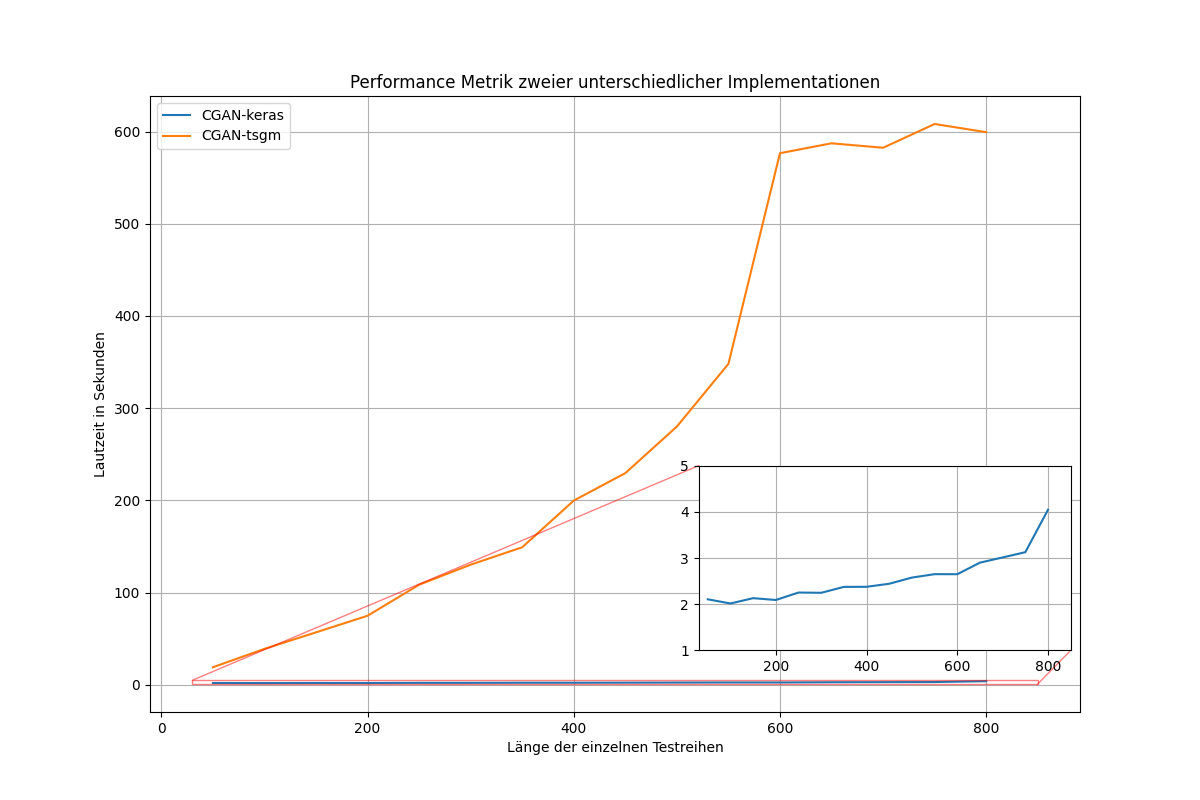
\includegraphics[width=\textwidth]{includes/figures/compare_run_time_iterations.png}
        \caption{Laufzeit des nativen CGAN Modells im Vergleich zur tsgm Implementierung in Abhängigkeit der Länge der Zeitreihen}
        \label{fig:compare_run_time_iterations}
    \end{minipage}\hfill
    \begin{minipage}{0.5\textwidth}
        \centering
        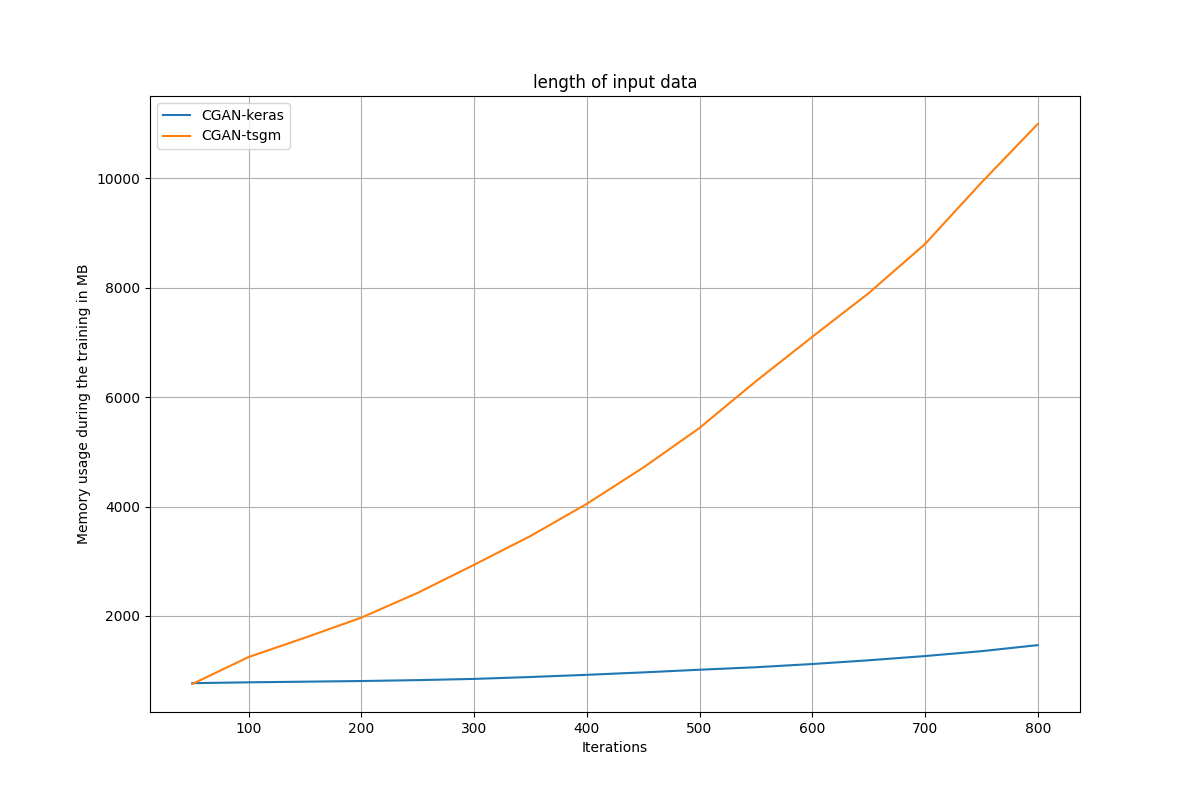
\includegraphics[width=\textwidth]{includes/figures/ram_usage_tsgm_vs_keras.png}
        \caption{RAM Auslastung des nativen CGAN Modells im Vergleich zur tsgm Implementierung in Abhängigkeit der Länge der Zeitreihen}
        \label{fig:compare_ram_usage}
    \end{minipage}
\end{figure}


Dennoch ist der nur sehr geringe Anstieg der Laufzeiten des Keras Modells sehr beeindruckend. Keras hat einen minimalen Anstieg, während der Anstieg der tsgm Modelle linear zur Anzahl der Iterationen ist.
Da der \ac{RAM} Verbrauch der tsgm Modelle sehr hoch war, wurde dieser auch gemessen. Hier ist auch wieder der Docker Container hilfreich, da die Isolation der Container dafür sorgt, dass der Verbrauch nicht durch andere Programme beeinflusst wird.
Wie in Abbildung \ref{fig:compare_ram_usage} zu sehen ist, ist selbst bei kleinen Modellen der \ac{RAM} Verbrauch der tsgm Modelle deutlich höher als der der nativen Modelle. Daher ist besonderst für diese eine vernünftige Vorverarbeitung wichtig,
da sonst weder die Laufzeit noch die Hardware Anforderungen von normalen Computern akzeptabel bzw ausreichen sind.


In Abbildung \ref{fig:train_time_compared} ist noch einmal der Verlauf aller getesteten Modelle zu sehen. Hier ist deutlich zu erkennen, dass die meisten tsgm Modelle deutlich mehr Zeit benötigen als die nativen Modelle.
\begin{figure}[ht]
    \centering
    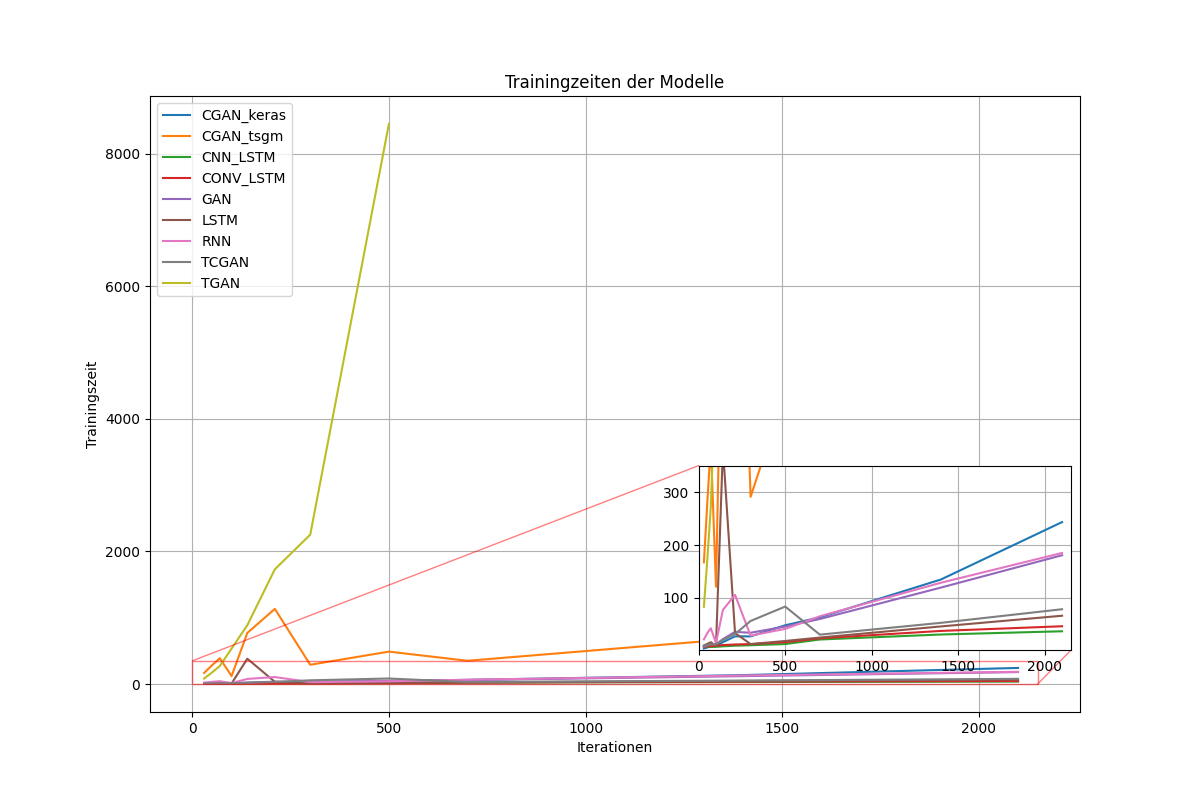
\includegraphics[width=1\textwidth]{includes/figures/graphs/train_time_compared.png}
    \caption{Laufzeit der einzelnen Modelle im Vergleich zur Anzahl der Iterationen}
    \label{fig:train_time_compared}
\end{figure}



\subsection{Performance Metriken der TSA Algorithmen}
Die Trainingszeiten der \ac{TSA} Algorithmen sind deutlich geringer als die der \ac{ML} Modelle, wie in Tabelle \ref{tab:trainingszeiten_tsa} zu sehen ist.
Der Cubic Spline Algorithmus ist hierbei der schnellste, da er nur eine Interpolation durchführt und keine weiteren Berechnungen benötigt.
Schaut man auf die anderen Modelle, so fällt Amira auf, dieser ist weitaus langsamer als die anderen Algorithem.
Dies liegt daran, dass Amira eine sehr komplexe Architektur besitzt und daher deutlich mehr Rechenleistung benötigt.

\begin{table}[ht]
    \centering
    \caption{Trainingszeiten der \ac{TSA} Algorithmen}
    \begin{tabular}{lrr}
        \toprule
        Algorithm & Iteration & Trainingszeit in Sekunden \\
        \midrule
        Amira     & /         & 0.452361                  \\
        Cubic     & /         & 0.004374                  \\
        EMD       & 0         & 0.038583                  \\
        EMD       & 1         & 0.038053                  \\
        EMD       & 2         & 0.040761                  \\
        EMD       & 3         & 0.039456                  \\
        SSA       & 0         & 0.013947                  \\
        SSA       & 1         & 0.014150                  \\
        SSA       & 2         & 0.012575                  \\
        SSA       & 3         & 0.012223                  \\
        \bottomrule
    \end{tabular}
    \label{tab:trainingszeiten_tsa}
\end{table}


\subsection{Auslastung der Hardware in Produktion}
Wie bereits vorher einmal angemerkt, sind die \ac{ML} Modelle deutlich fordernder als es die \ac{TSA} Algorithmen sind.

Um dies aber einmal in Produktion sehen zu können, wurde für die Django \ac{API} ein separater Prometheus Importer für die CPU Auslastung geschrieben.
Dieser sammelt in 2 Sekunden Intervallen die Auslastung der CPU und wird über das \ac{ELK} Stack visualisiert.
Leider konnte dies aber nicht auf gleiche Art und Weise mit der RAM-Auslastung getestet werden, da Python's Speichermanagement und seine Garbage Collection nicht vorhersehbar sind. Trotz separater Reinigung zeigte sich kein wirklicher Anstieg der RAM-Auslastung oder stieg nach Abschluss des Trainingsprozesses sogar noch.

In Abbildung \ref{fig:cpu_usage_in_container}

\begin{figure}[ht]
    \centering
    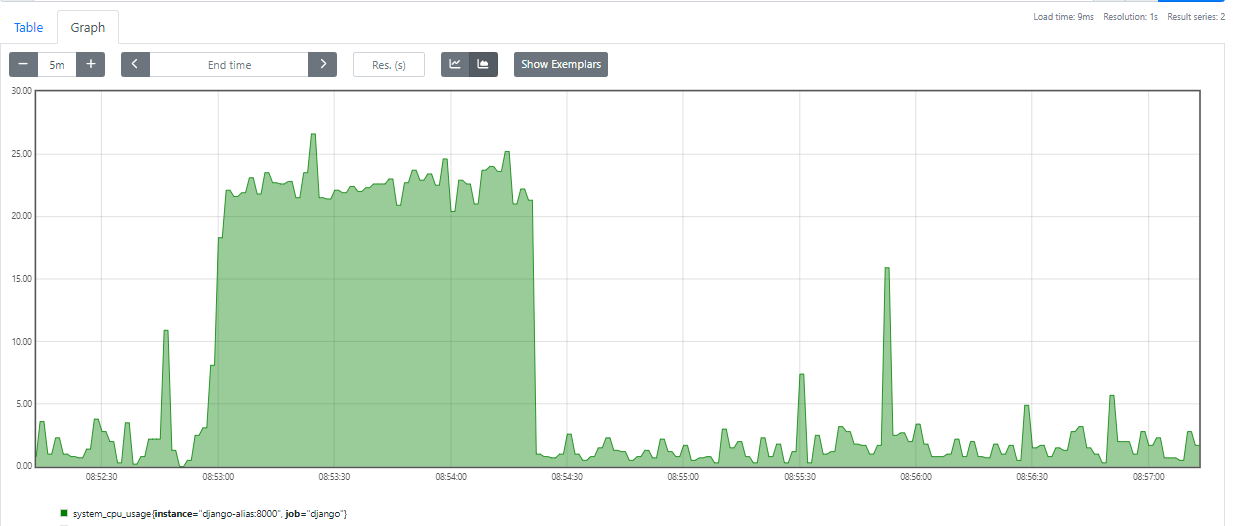
\includegraphics[width=1\textwidth]{includes/figures/tooling/performance.png}
    \caption[\ac{CPU} Auslastung der Django API]{Der erste große Anstieg zeigt die Auslastung während des Trainings eines GAN Modells (Zwischen 08:53 und 08:54), der kurze Anstieg während 08:56 zeigt die CPU Auslastung während der SSA-Algorithmus aufgerufen wurde}
    \label{fig:cpu_usage_in_container}
\end{figure}










\subsection{Ähnlichkeit der Zeitreihen der \ac{ML} Modelle}
\label{sec:similarity_of_time_series}
Um die Ähnlichkeit der Zeitreihen zu bewerten wurden die in Sektion \ref{sec:non_statistical_measures} vorgestellten Metriken genutzt.
Diese Metriken zeigen direkt, dass Beispielsweise die Ähnlichkeit der \ac{ML} Modelle basierend auf Ihrer Architektur sehr unterschiedlich ist.
Rekursive Modelle wie beispielsweise das \ac{LSTM} Modell, zeigen eine sehr viel schnellere Annährung zu den realen Daten als die generativen Modelle.
Da diese aber versuchen eine Funktion zu erlernen, welche die Daten generiert anstatt Muster aus einem Fenster an vorherigen Werten zu lernen und daraus den nächsten Wert zu berechnen, ist dies wenig verwunderlich.
Interessant ist aber, dass über einen Anstieg der Iterationen die Genauigkeit der generativen Modelle zwar tendenziell besser wird, aber von Außreißern unterbrochen wird.
Um dennoch eine vernünftige Vergleichbarkeit zu erziehlen, wurden alle Algorithmen mit der gleichen Anzahl an Iterationen trainiert. Sie wurden in Intervallen von 10, 30, 50, 70, 100, 140, 210, 300, 500 getestet. Die nativen Keras Modelle wurden noch in Intervallen von 700, 1400 und 2100 Iterationen getestet.
Für die tsgm Modelle war dies nur Teilweise noch möglich, da sich die Laufzeit im Extremfall des \ac{TGAN}s schon auf über 1h16min für 500 Iterationen belief. Da hier auch die Trainingszeit je Iteration Anstieg hätte dies, gerade über mehrere Trainingsdatensätze, zu lange gedauert und wäre daher wenig sinnvoll.

Interessante Punkte sind beispielsweise die Laufzeit der Modelle, die Anzahl an Iterationen im Verhähltnis zur Wasserstein Distanz und die Anzahl an Iterationen im Verhähltnis zur Vektor Distanz. Andere interessante Punkte sind beispielsweise das Privatsphäre Maß auch in ein Verhähltnis zur Distanz und zur Laufzeit zu setzten.
Gerade der letzte Punkt sollte interessante Ergebnisse liefern, da die generativen Modelle eine sehr hohe Laufzeit haben und daher auch ein hohes Maß an Privatsphäre bieten sollten, aber die Distanz zum original nicht zu gering sein soll, da es sonst diese nicht gut genug nachbildet.

\subsubsection{Analyse der rekursiven Modelle}
\paragraph{\textbf{RNN}}
Betrachtet man die Grafik des RNN, zeigt sich eine erhebliche Fluktuation, aber im Vergleich zu anderen Modellen weist es einen sehr stabilen Wert auf. Die Wasserstein-Distanz divergiert bei 500 Iterationen,
erreicht aber hier nur einen Wert von 0,124 – eine sehr gute Annäherung. Ähnlich verhält es sich mit der Vektordistanz, die bei nur 0,02 liegt. Beide Werte, auch die sehr niedrige Standardabweichung,
deuten auf eine hohe Übereinstimmung mit den Originaldaten hin, und das fast unmittelbar. Eine recht niedrige \ac{MIA}-Metrik zeigt ebenfalls, dass das Modell die Privatsphäre nicht ausreichend schützt und Rückschlüsse auf Originalmuster zulässt.


\paragraph{\textbf{LSTM}}
Die Daten dieses Modells verhalten sich interessant. Die Wasserstein-Distanz steigt kontinuierlich an, zeigt also eine Entfernung von den Originaldaten, allerdings in einem, verglichen mit anderen Modellen,
langsamen und geringen Rahmen. Die Standardabweichung steigt ähnlich zur Wasserstein-Distanz; gleiches gilt für die \ac{MIA}-Metrik, die leider dennoch sehr gering ist. Die Vektordistanz liegt fast bei 0 und zeigt einen Ausreißer,
der sich schnell wieder einpendelt. Aus den Daten des Mann-Whitney-U-Tests lässt sich ein Trainingseffekt erkennen, aber die P-Werte fallen nie unter die 0,05-Marke.


\begin{figure}[ht]
    \centering
    \begin{minipage}{0.5\textwidth}
        \centering
        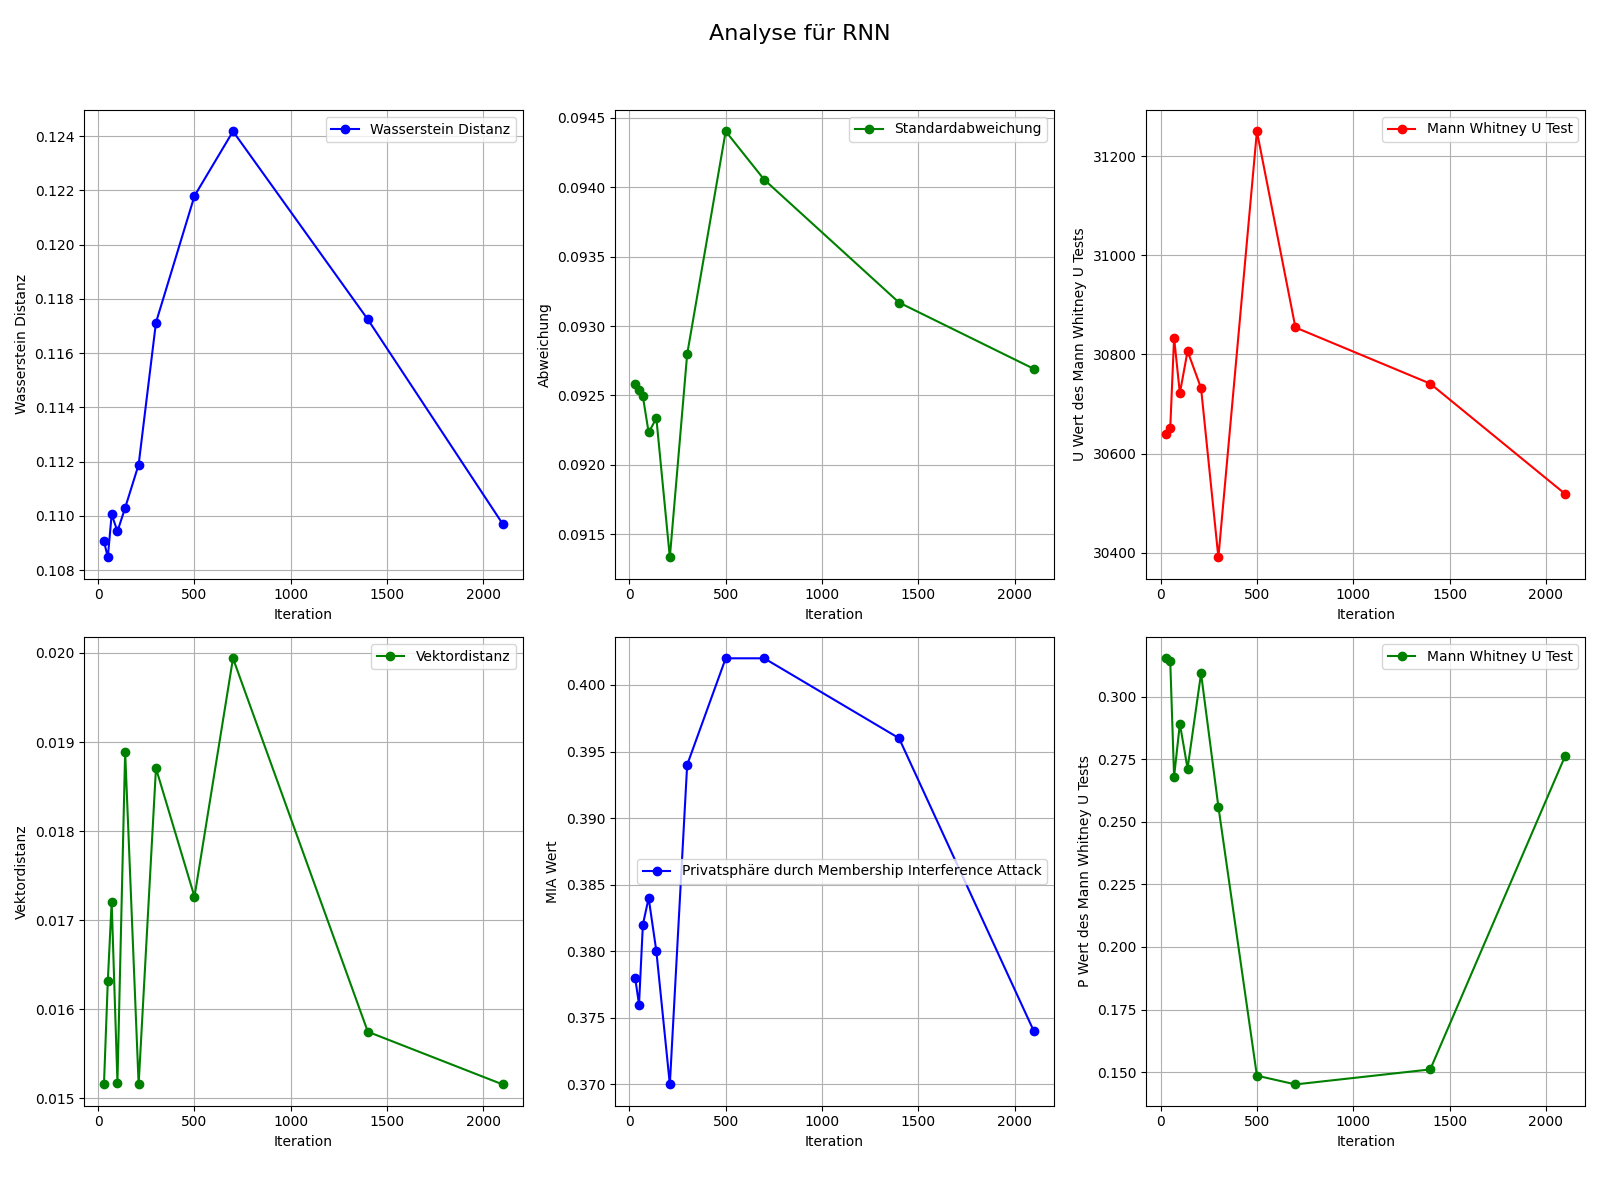
\includegraphics[width=\textwidth]{includes/figures/graphs/RNN_analysis.png}
        \caption{Analyse des RNN Modells}
        \label{fig:graphs_rnn_analysis}
    \end{minipage}\hfill
    \begin{minipage}{0.5\textwidth}
        \centering
        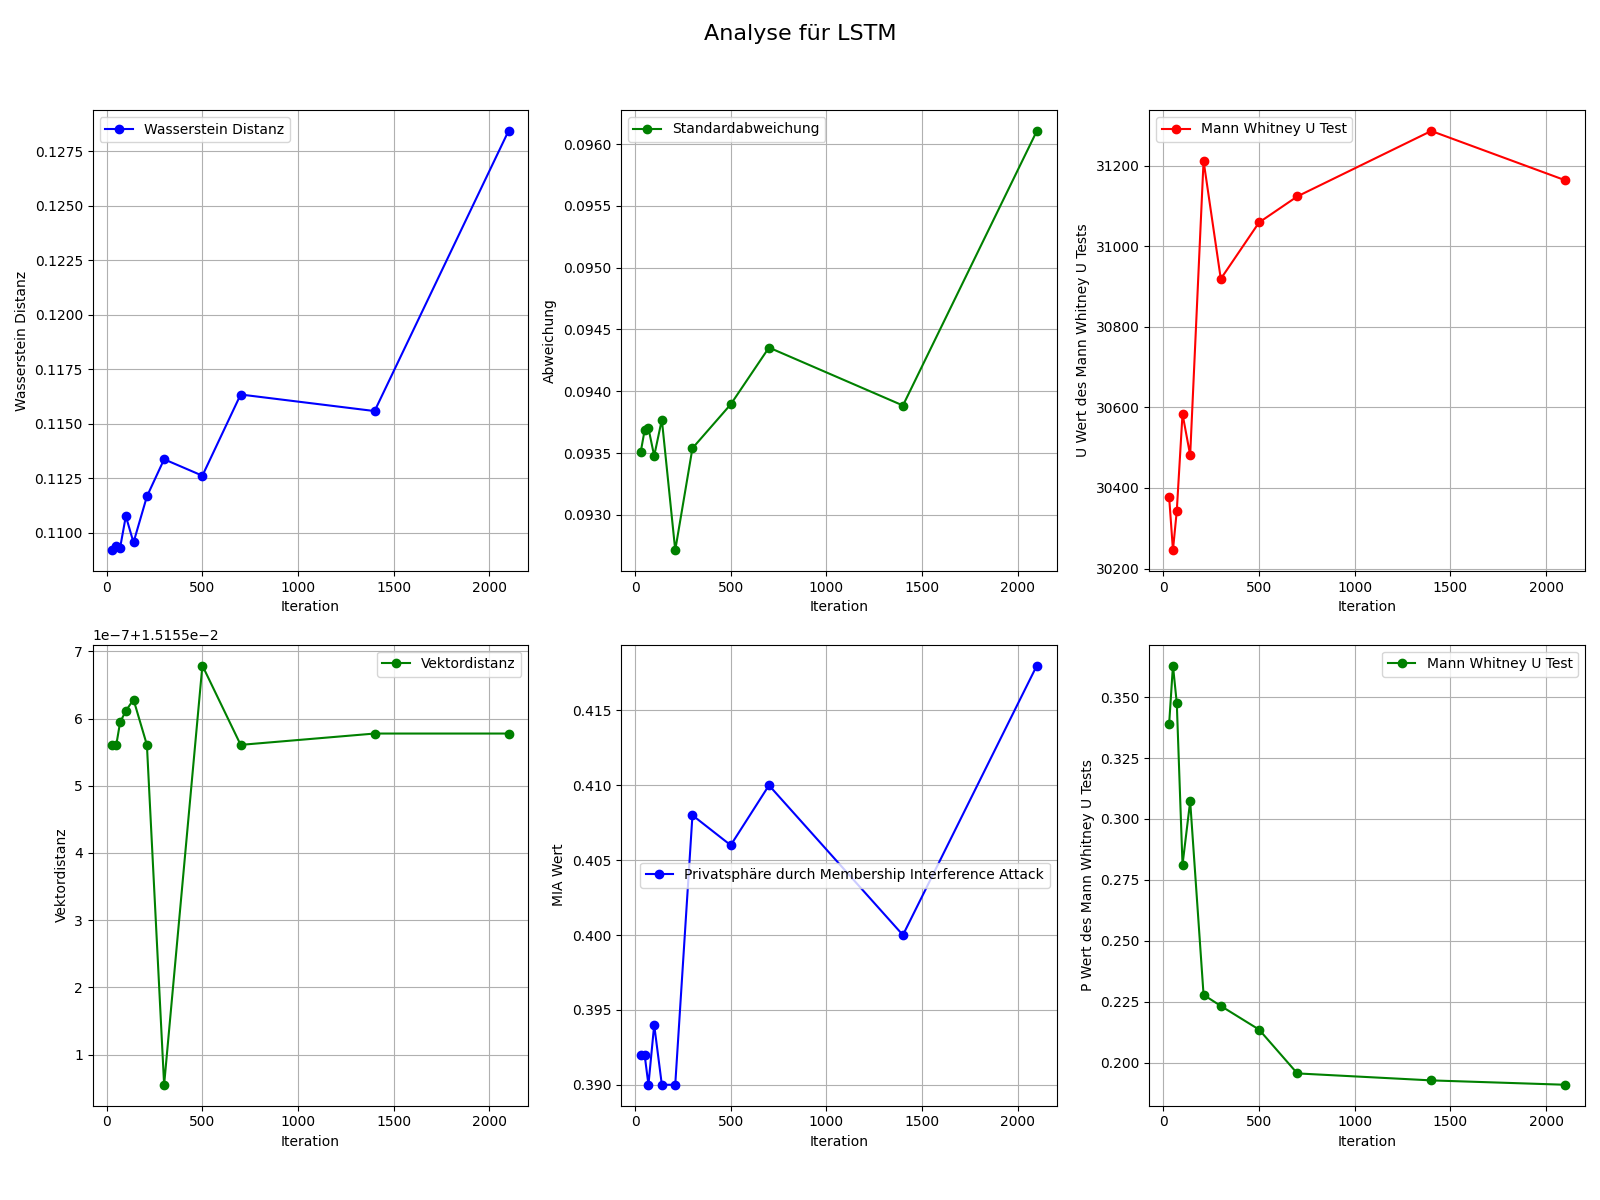
\includegraphics[width=\textwidth]{includes/figures/graphs/LSTM_analysis.png}
        \caption{Analyse des LSTM Modells}
        \label{fig:graphs_lstm_analysis}
    \end{minipage}
\end{figure}




\paragraph{\textbf{Convolutional LSTM}}
Die Wasserstein-Distanz dieses Modells startet sehr hoch, fällt schnell ab und fluktuiert, bevor sie sich bei einem Wert von 0,1 einpendelt. Das Modell kann also sehr schnell die Verteilung der Originaldaten erfassen.
Ähnlich verhält es sich mit der Vektordistanz, die ebenfalls hoch beginnt und sich etwas langsamer einpendelt als die Wasserstein-Distanz. Mit einem Wert von ungefähr 0,45 ist sie aber dennoch akzeptabel.
Die \ac{MIA}-Metrik und die Standardabweichungen folgen einem ähnlichen Verlauf: Sie starten hoch, fallen, fluktuieren und pendeln sich ein. Am Ende erreicht das Modell nur einen Wert von 0,65 in der \ac{MIA},
was recht gut ist. Die Ergebnisse des Mann-Whitney-U-Tests zeigen niedrige P-Werte, die aber nie den Schwellwert von 0,05 erreichen. Das Modell erreicht somit nie eine exakte Annäherung an die Originaldaten,
was durchaus erwünscht sein kann. Der starke Anstieg um Iteration 1400 sollte durch weitere Tests untersucht werden.

\paragraph{\textbf{CNN LSTM}}
Die Wasserstein-Distanz zeigt bei ungefähr 700 Iterationen eine signifikante Spitze. Da der Wert über mehrere Datensätze hinweg berechnet wurde und die Extrema nicht stärker als bei anderen Iterationen abweichen,
scheint das Modell in diesem Bereich zu divergieren. Die Standardabweichung zeigt keine Auffälligkeiten. Die Vektordistanz verhält sich ähnlich wie die Wasserstein-Distanz, nur mit einem niedrigeren Wert, der gegen Ende
der Iterationen wieder ansteigt. Interessant ist der Abfall der \ac{MIA}-Metrik, als die Wasserstein- und Vektordistanz ansteigen, was etwas kontraintuitiv erscheint. Die Werte des Mann-Whitney-U-Tests zeigen ähnliche Muster
und normalisieren sich nach der initialen Trainingsphase.

\begin{figure}[ht]
    \centering
    \begin{minipage}{0.5\textwidth}
        \centering
        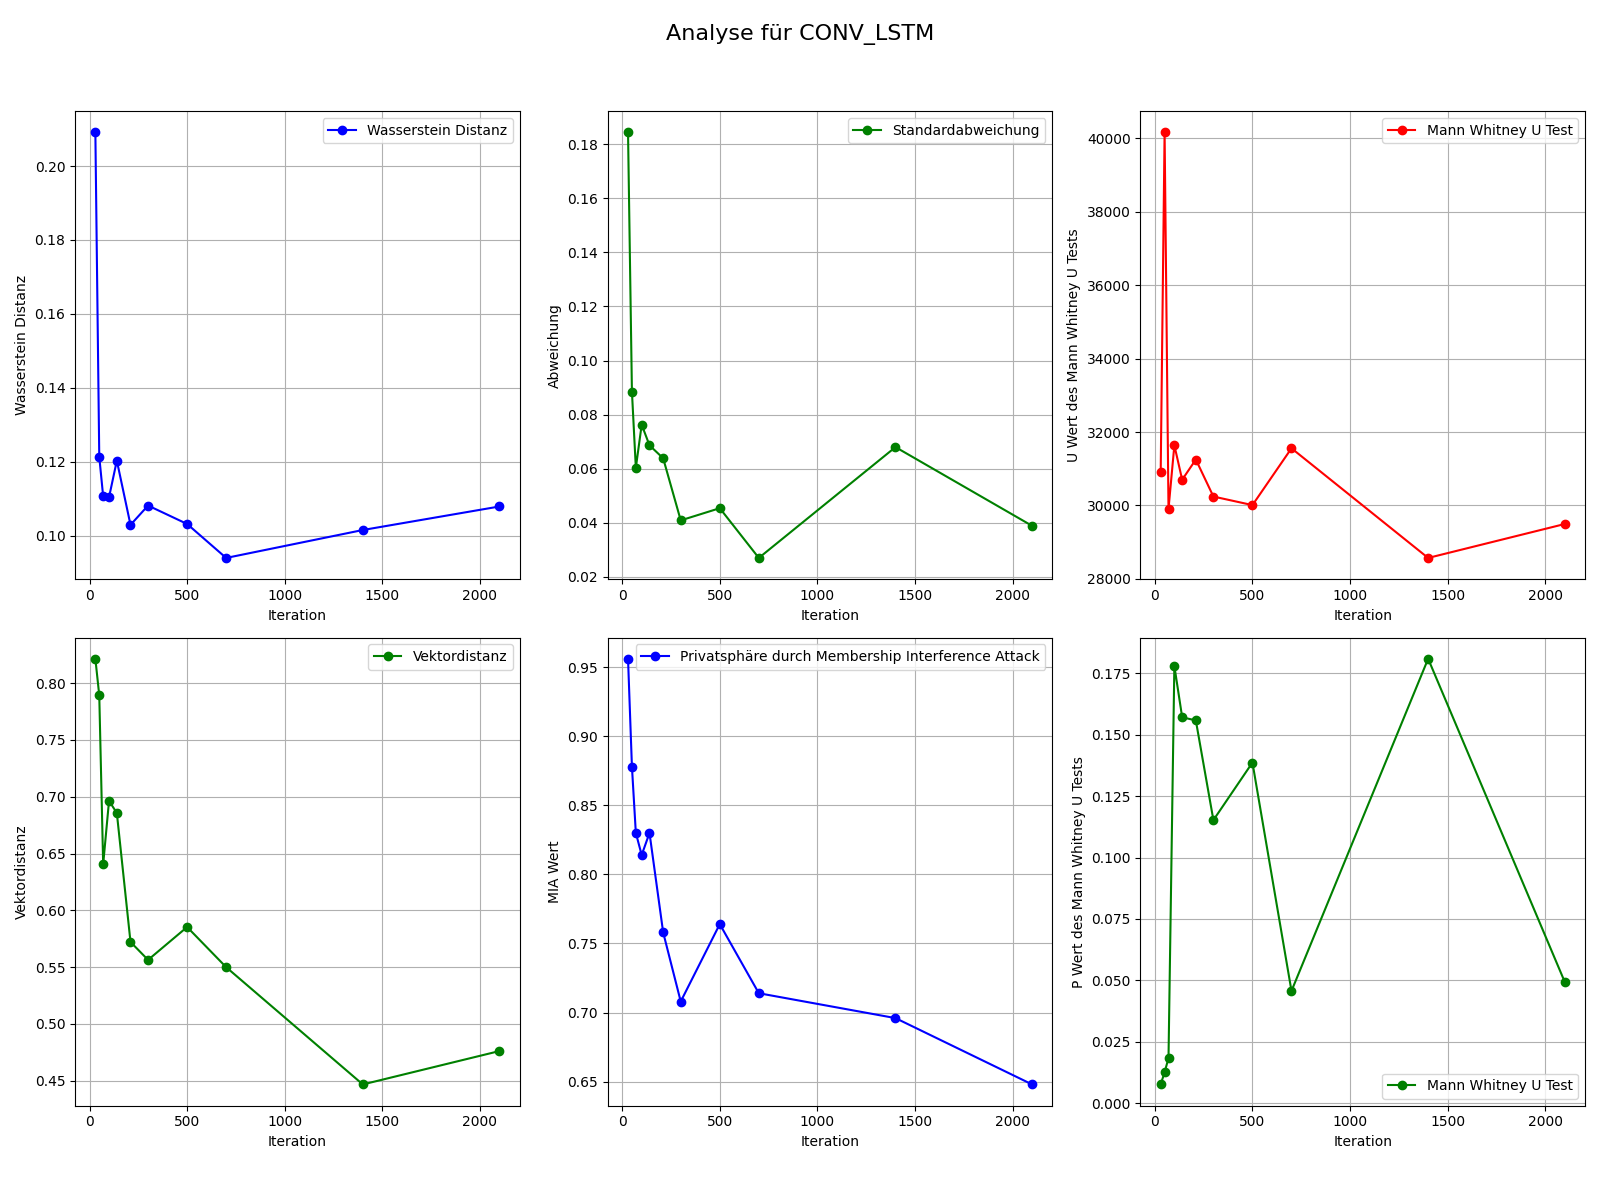
\includegraphics[width=\textwidth]{includes/figures/graphs/CONV_LSTM_analysis.png}
        \caption{Analyse des Convolutional LSTM Modells}
        \label{fig:graphs_conv_analysis}
    \end{minipage}\hfill
    \begin{minipage}{0.5\textwidth}
        \centering
        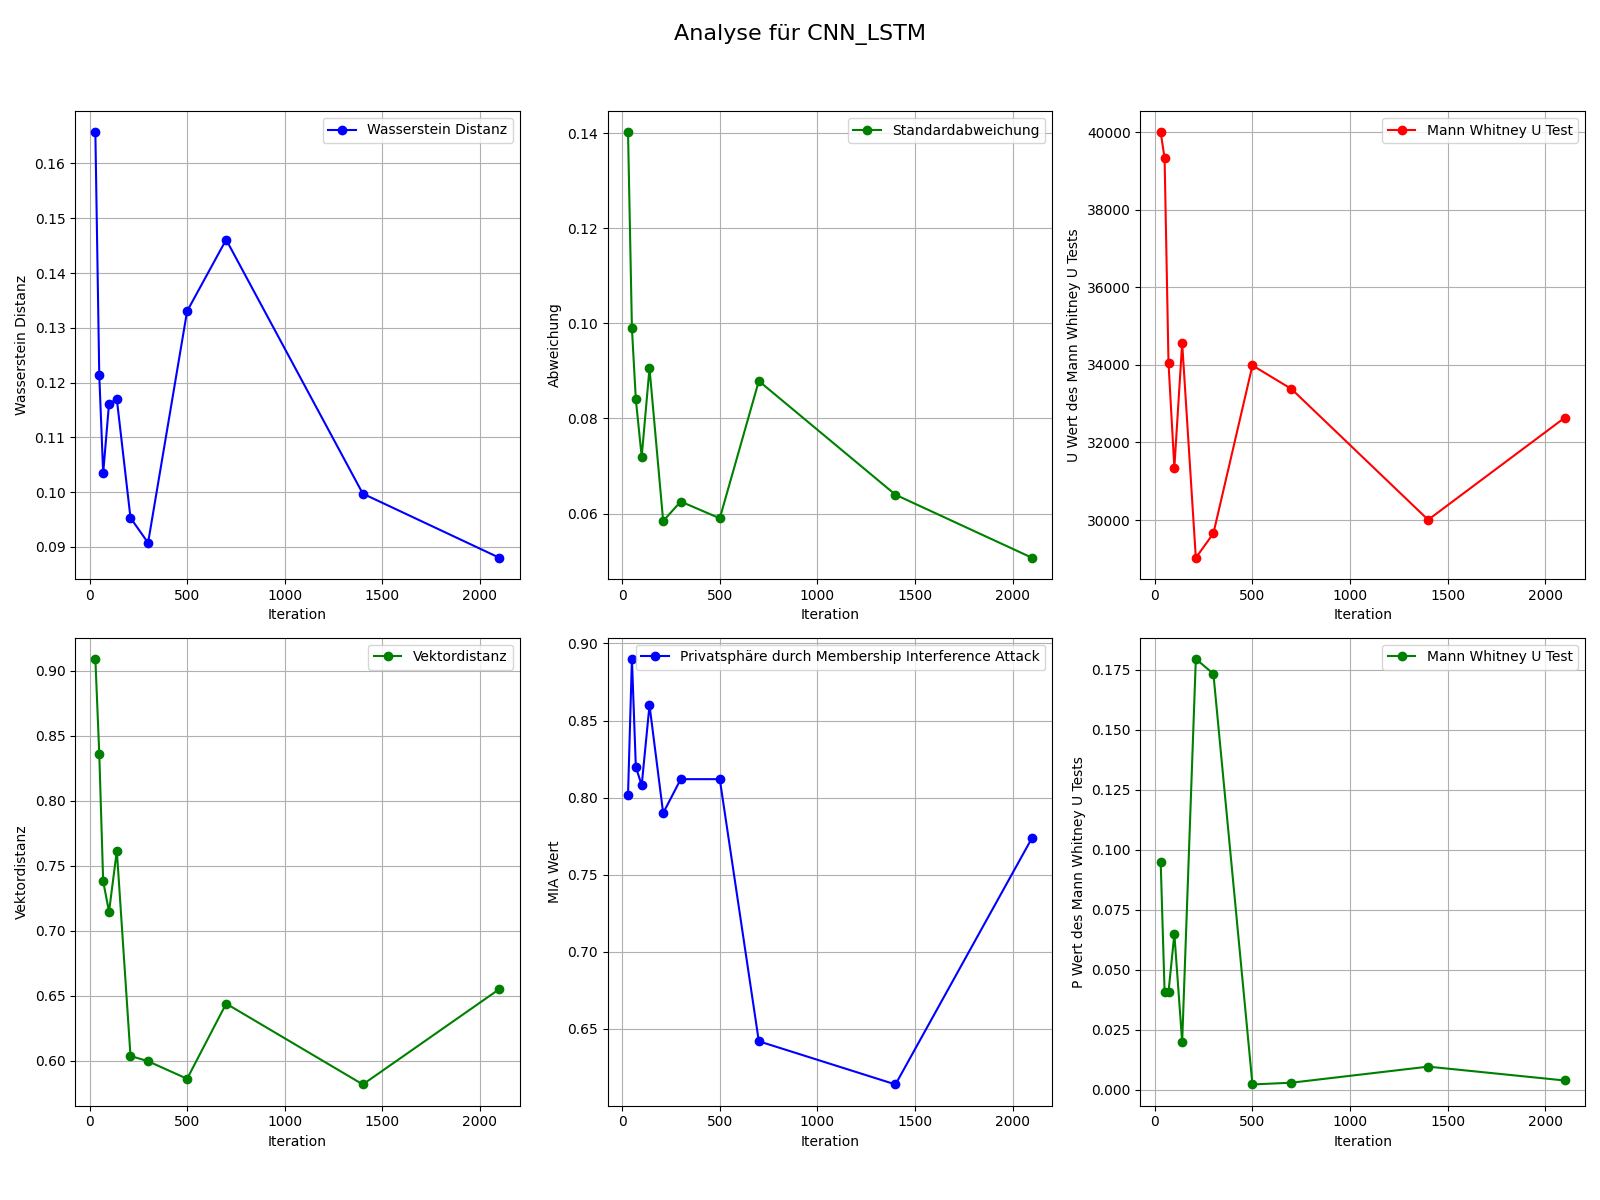
\includegraphics[width=\textwidth]{includes/figures/graphs/CNN_LSTM_analysis.png}
        \caption{Analyse des CNN LSMT Modells}
        \label{fig:graphs_cnn_analysis}
    \end{minipage}
\end{figure}



\subsubsection{Analyse der generativen Modelle}

\paragraph{\textbf{GAN}}
Das GAN zeigte eine signifikante anfängliche Verbesserung und verringerte schnell die Diskrepanz in der Verteilung zwischen generierten und realen Daten, wie die Wasserstein- und Vektordistanz-Metriken anzeigen.
Die Standardabweichung des Modells nimmt ab, was auf eine Verbesserung der Konsistenz der Datengenerierung hindeutet.

Schwankungen in der Mann-Whitney-U-Test-Statistik und ihren P-Werten weisen auf Momente der Divergenz zwischen den synthetischen und realen Datenverteilungen hin, was auf eine potenzielle Überanpassung oder
Instabilität des Modells im Laufe des Trainings schließen lässt. Die \ac{MIA}-Werte deuten auf eine erhöhte Anfälligkeit für Inferenzangriffe hin, sind aber verglichen mit anderen Algorithmen recht gut.

Die anfänglichen und schnellen Erfolge des Modells zeigen einen schnellen Lernprozess, der ab ungefähr 1000 Iterationen stagniert.


\paragraph{\textbf{TGAN}}
Das TGAN zeigte gute Fähigkeiten bei der Annäherung an reale Datenverteilungen, wie die Trends der Wasserstein- und Vektordistanz zeigen. Bereits die ersten Iterationen des Modells zeigen Fortschritte bei der
Generierung von synthetischen Daten. Gleichzeitig zeigte das TGAN Schwankungen in den Datenschutzmetriken, was eine Konsequenz der schnellen Verbesserung der Wasserstein- und Vektordistanzmetriken sein kann.

Die beobachtete Standardabweichung und die Mann-Whitney-U-Test-Statistiken wiesen zudem auf Perioden signifikanter Verbesserung und Stabilität in der Leistung des TGAN hin. Diese Metriken wiesen jedoch auch auf
Fälle hin, in denen die Ergebnisse des Modells von den gewünschten Ergebnissen abwichen, was auf potenzielle Bereiche zur Verfeinerung hindeutet.


\begin{figure}[ht]
    \centering
    \begin{minipage}{0.5\textwidth}
        \centering
        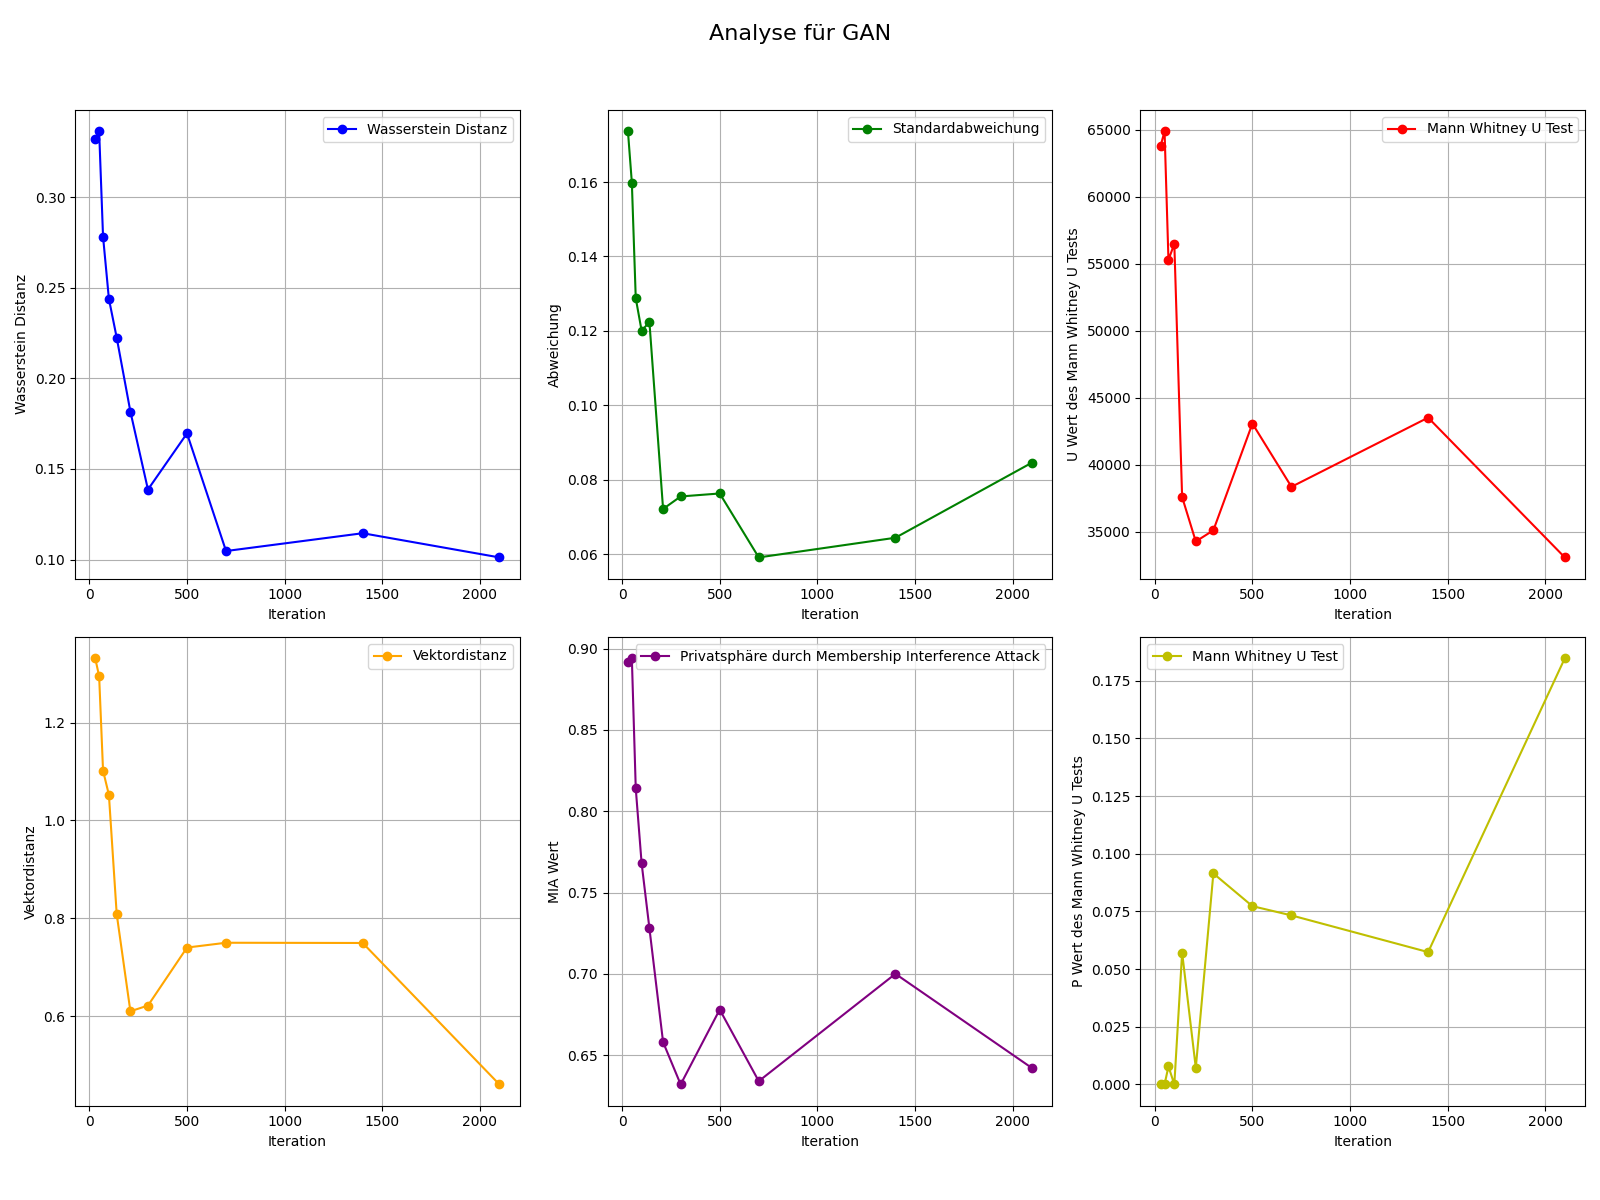
\includegraphics[width=\textwidth]{includes/figures/graphs/GAN_analysis.png}
        \caption{Analyse des GAN Modells}
        \label{fig:graphs_gan_analysis}
    \end{minipage}\hfill
    \begin{minipage}{0.5\textwidth}
        \centering
        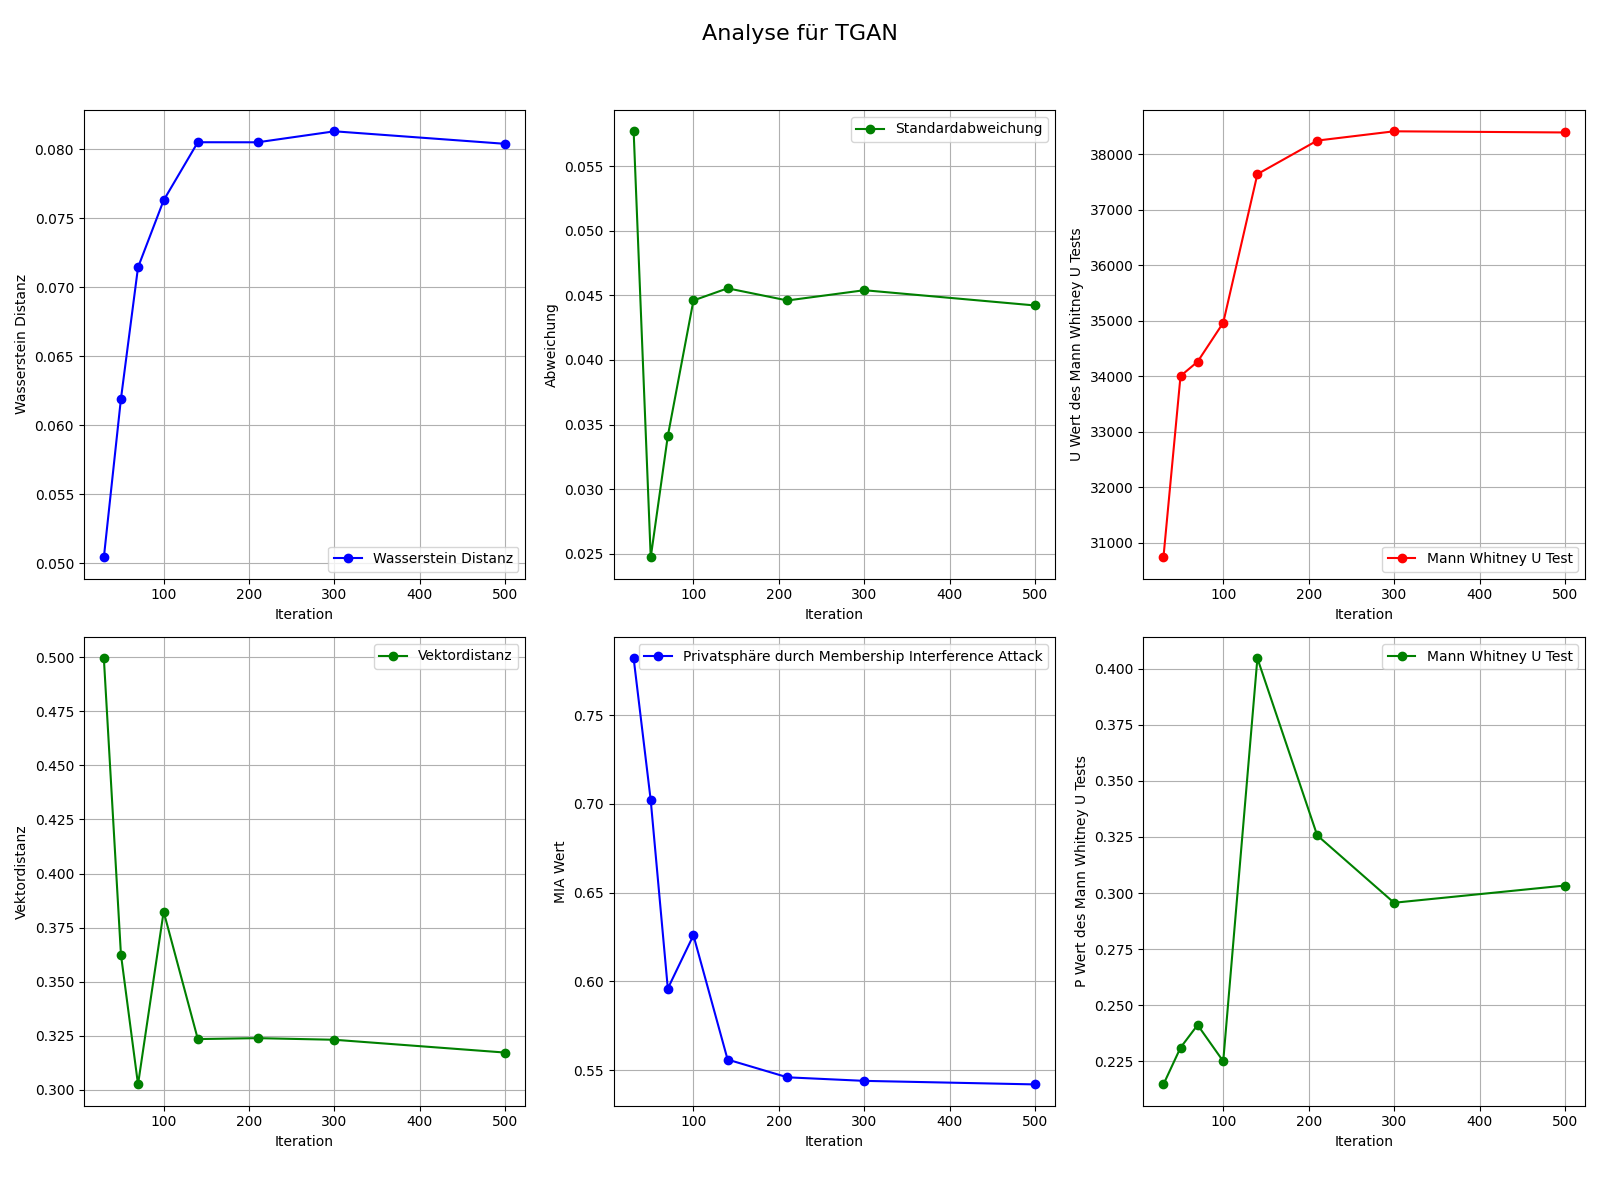
\includegraphics[width=\textwidth]{includes/figures/graphs/TGAN_analysis.png}
        \caption{Analyse des TGAN Modells}
        \label{fig:graphs_tgan_analysis}
    \end{minipage}
\end{figure}


\paragraph{\textbf{TCGAN}}
Während des gesamten Trainingsprozesses zeigte das TCGAN eine gute Verbesserung mit einem abfallenden Lerneffekt, wie die Werte der Standardabweichung, Vektordistanz und Wasserstein-Distanz anzeigen.

Bezüglich der Privatsphäre zeigte das TCGAN eine schlechte Leistung, wie die \ac{MIA}-Metrik zeigt.

Darüber hinaus wiesen die P-Werte des Mann-Whitney-U-Tests auf Momente hin, in denen sich die synthetischen Daten signifikant von den Originaldaten unterschieden, was Fragen hinsichtlich der Fähigkeit des Modells aufwirft,
Daten mit konsistenten statistischen Eigenschaften über Iterationen hinweg zu generieren.
\begin{figure}[ht]
    \centering
    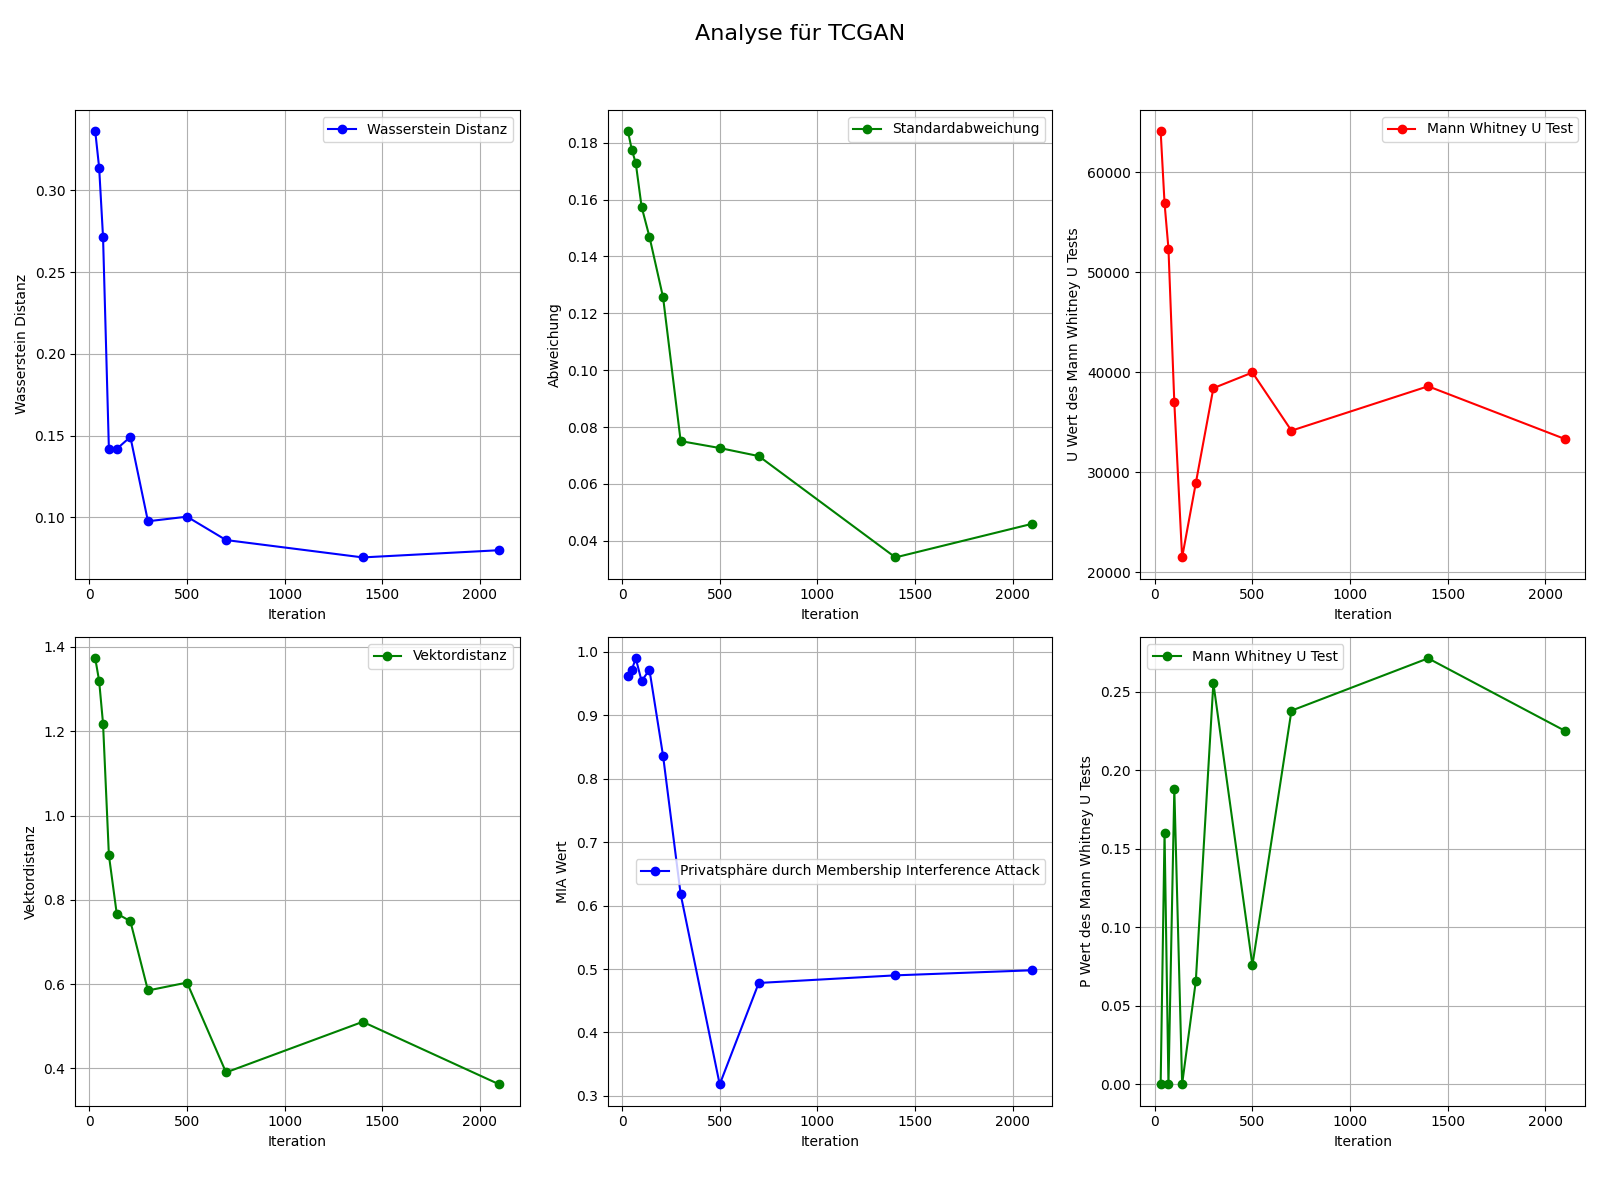
\includegraphics[width=1\textwidth]{includes/figures/graphs/TCGAN_analysis.png}
    \caption{Analyse des TCGAN Modells}
    \label{fig:graphs_tcgan_analysis}
\end{figure}


\paragraph{\textbf{CGAN-keras}}
Die CGAN-Keras zeigten einen sehr guten Start mit einer steilen Verbesserung des Wasserstein-Abstands und einem erstaunlich niedrigen Ausgangswert. Die Vektordistanz zeigt einen ähnlichen Verlauf, nähert sich extrem schnell den Daten an und
entfernt sich dann wieder. Hier ist eine hohe Fluktuation zu beobachten. Trotzdem sind die Standardabweichungen sehr gering und die Privatsphäre-Metriken zeigen einen durchaus guten Wert mit einer steigenden Tendenz.
Die Analyse der Mann-Whitney-U-Test-Statistiken und der P-Werte ergab jedoch Zeiträume, in denen die statistischen Eigenschaften der synthetischen Daten signifikant von denen der realen Daten abwichen, während zu manchen Zeiten der Schwellwert von 0,05 unterschritten wurde.

\paragraph{\textbf{CGAN-tsgm}}
Die CGAN-Variante der tsgm-Bibliothek zeigt ähnlich gute und schnelle Annäherungen und Trainingsfortschritte wie die keras-Variante. Nach einer rapiden Lernphase pendeln sich die Werte ein und zeigen eine gute Annäherung an die Originaldaten,
wie sich anhand der Wasserstein- und Vektordistanz sowie der Standardabweichung ablesen lässt. Leider zieht das gute Erlernen auch Konsequenzen für die Privatsphäre nach sich, da die \ac{MIA}-Metrik einen sehr niedrigen Wert zeigt.


\begin{figure}[ht]
    \centering
    \begin{minipage}{0.5\textwidth}
        \centering
        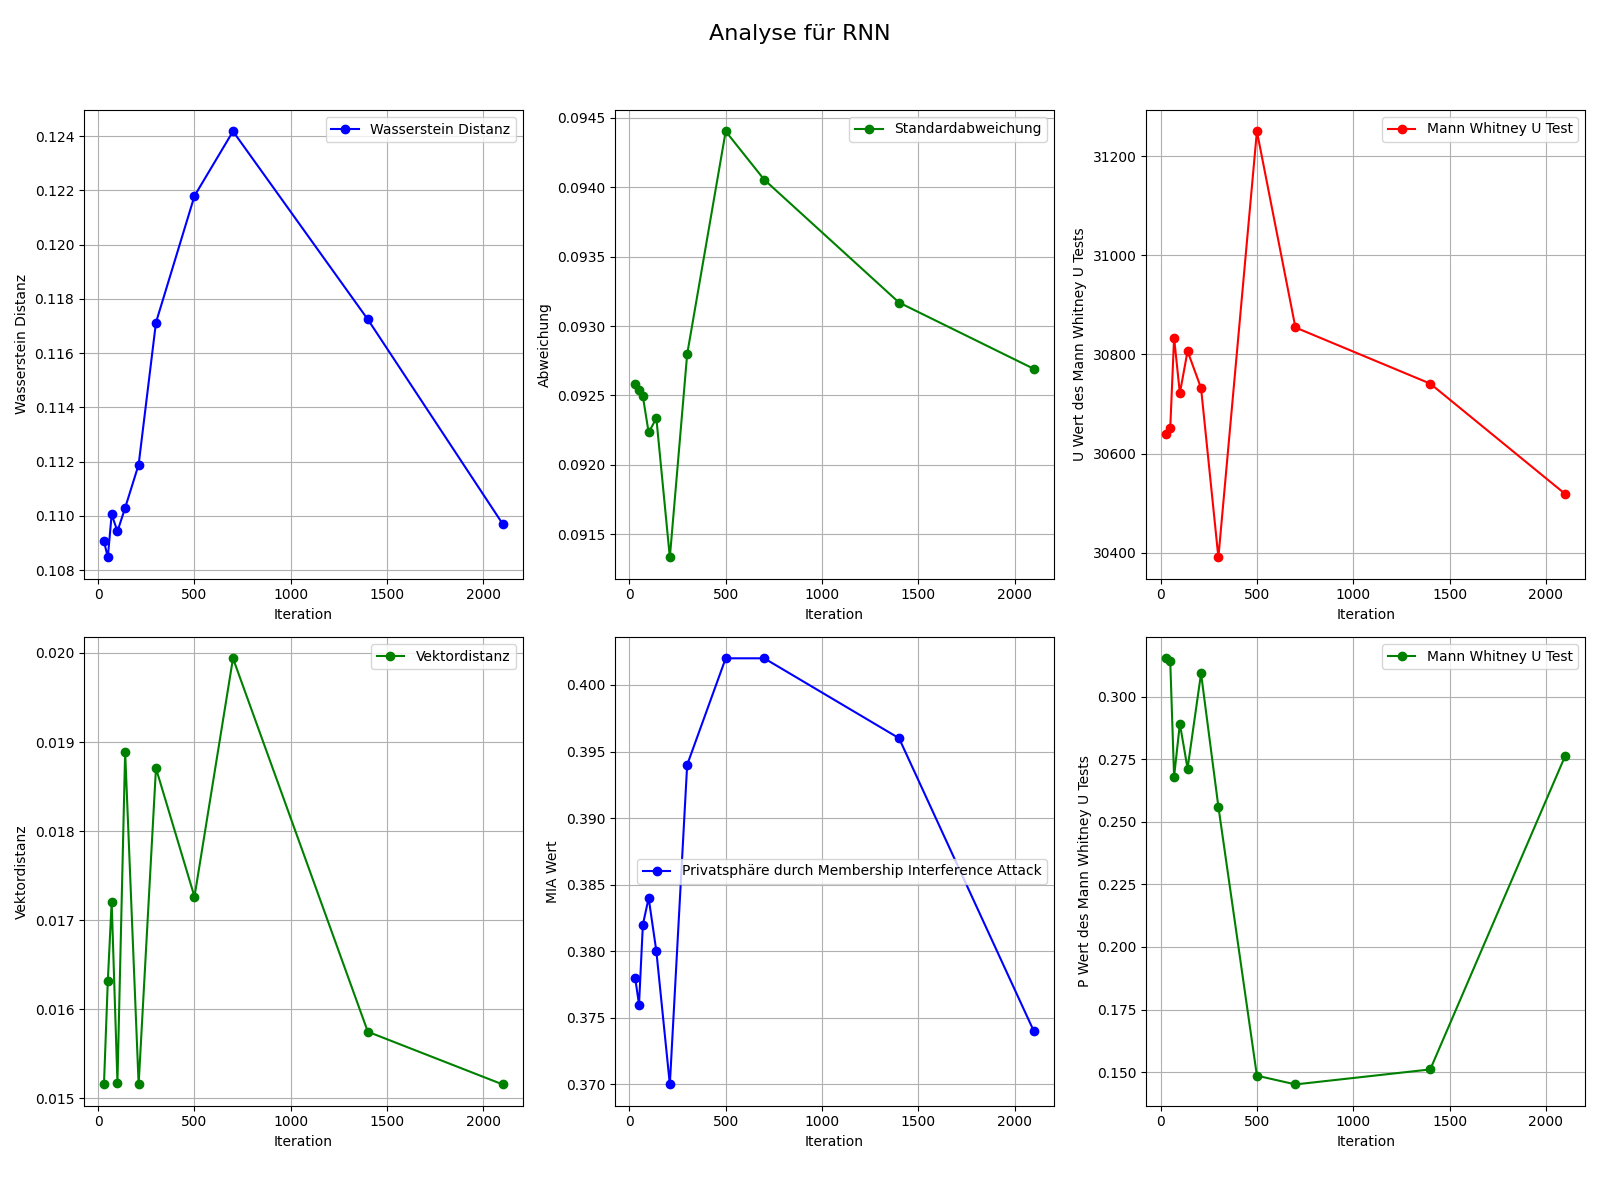
\includegraphics[width=\textwidth]{includes/figures/graphs/RNN_analysis.png}
        \caption{Analyse des CGAN tsgm Modells}
        \label{fig:graphs_cgan_tsgm_analysis}
    \end{minipage}\hfill
    \begin{minipage}{0.5\textwidth}
        \centering
        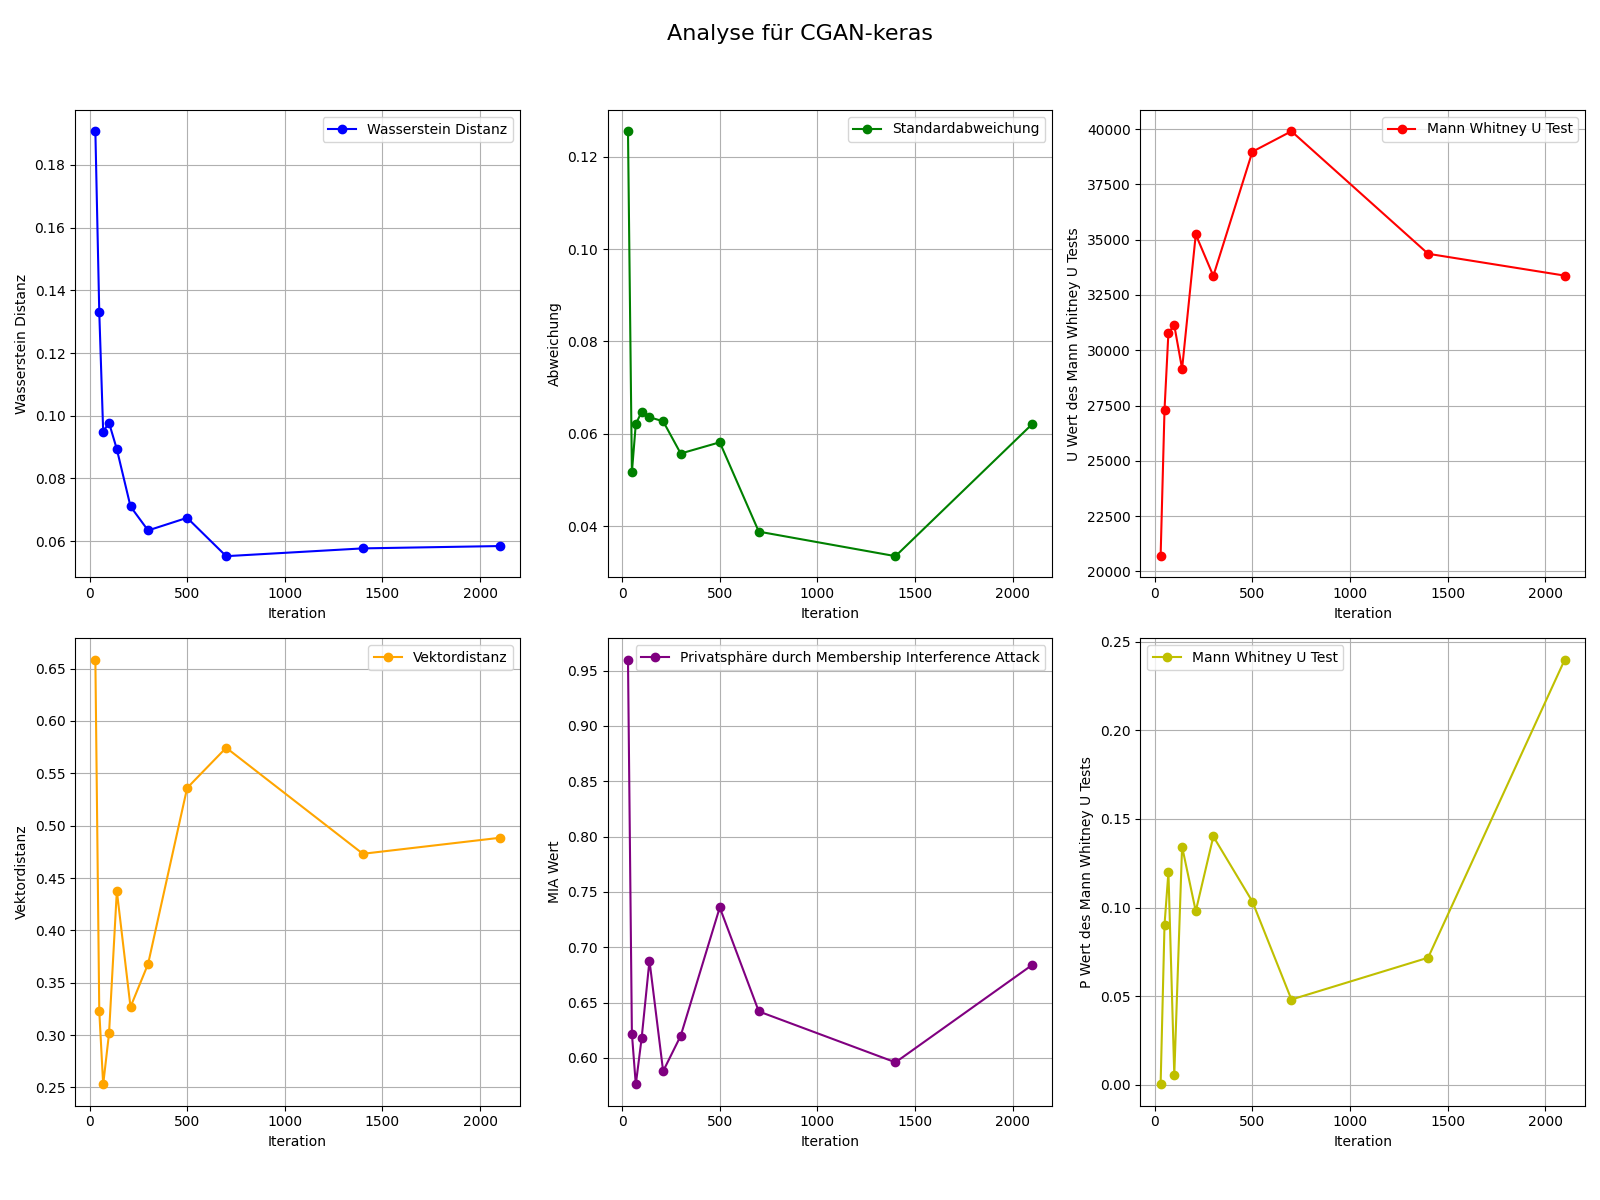
\includegraphics[width=\textwidth]{includes/figures/graphs/CGAN-keras_analysis.png}
        \caption{Analyse des CGAN Keras Modells}
        \label{fig:graphs_cgan_keras_analysis}
    \end{minipage}
\end{figure}




Da in den vorherigen Abschnitten primär die reinen Verteilungen über verschiedene Datensätze gezeigt wurden, ist es auch interessant zu sehen, wie sich die einzelnen Modelle auf die einzelne Datensätze auswirken.
Da die Modelle (mit ausnahme der tsgm Modelle) in der Lage sind spezifisch für die einzelnen Datensätze passende synthetische Varianten zu generieren, lässt sich die jeweilige Iteration eine Histogramms der synthetischen Daten erstellen, in dem sowohl die Verteilung als auch die direkten Werte verglichen werden.

Wie Anhand der in Abbildung \ref{fig:sinus_histogram} und \ref{fig:sinus_histogram_compare} gezeigten Histogramme zu sehen ist, sind die synthetischen Daten sehr gut an die Originaldaten angepasst. Es gibt, auch nach etwa 2100 Iterationen noch unterschiede im CGAN-keras Modell zu sehen, diese sind aber nur minimal, da es aber auch  das Ziel war die synthetischen Daten dem original nur anzunähern, scheint dieses Ergebnis doch durchaus gut.
\begin{figure}[ht]
    \centering
    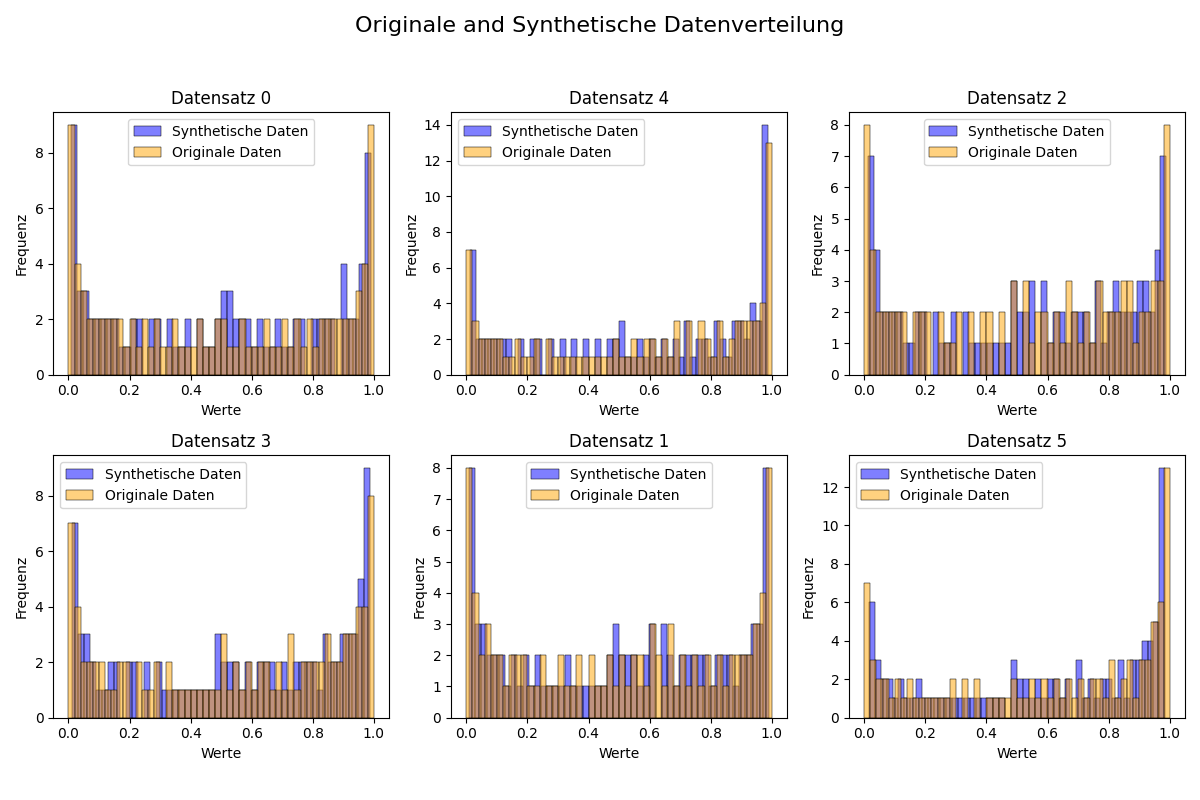
\includegraphics[width=1\textwidth]{includes/figures/graphs/sinus_plot_histogram.png}
    \caption{Verteilungen des jeweiligen einzelnen Trainingsdaten zu ihren synthetischen Varianten}
    \label{fig:sinus_histogram}
\end{figure}


\begin{figure}[ht]
    \centering
    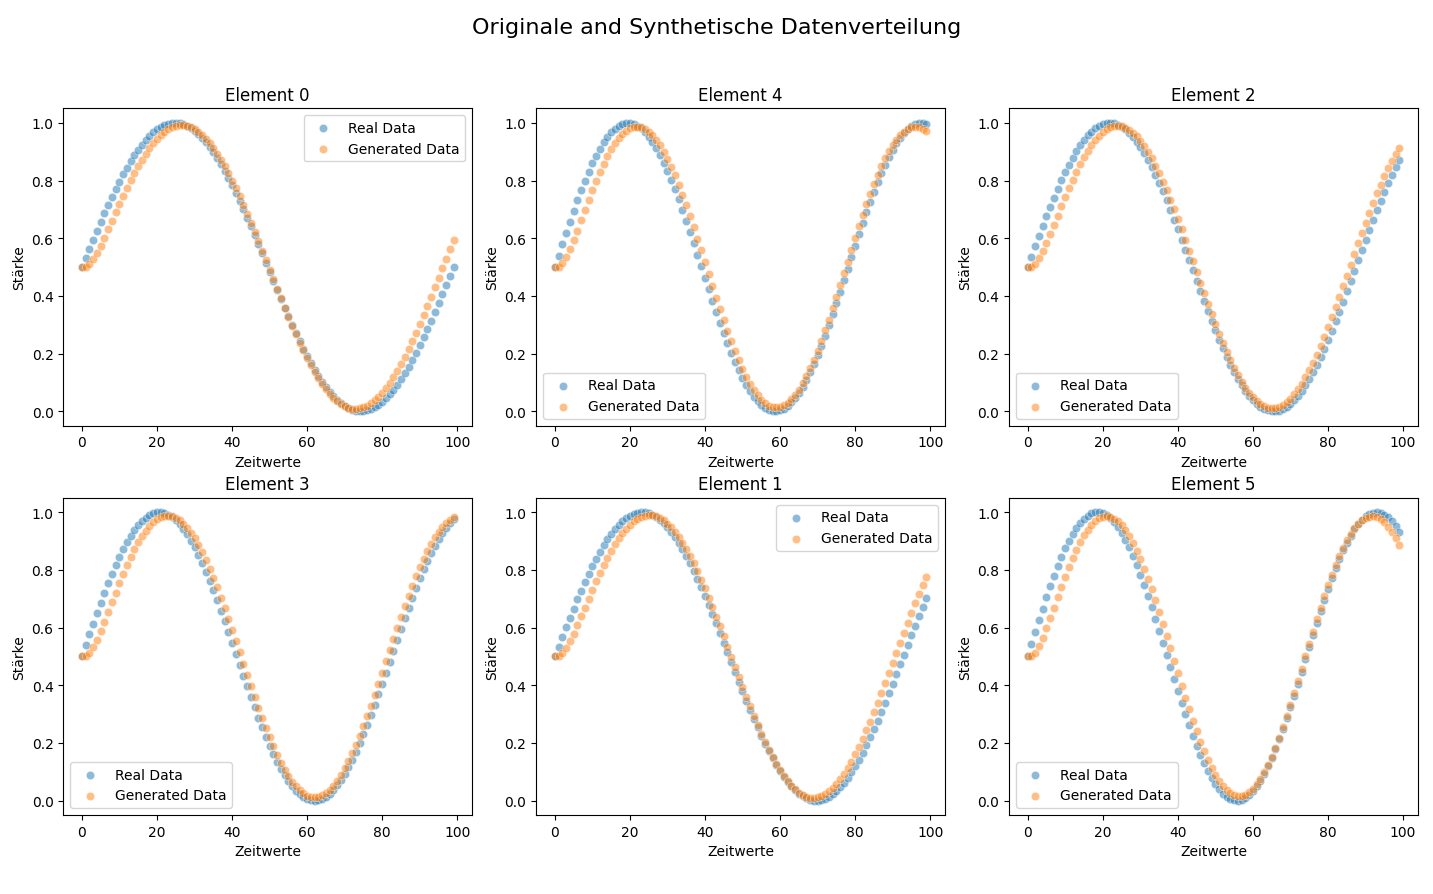
\includegraphics[width=1\textwidth]{includes/figures/graphs/sinus_plot_histgram_compare.png}
    \caption{Vergleich der einzelnen Trainingdaten zu ihren synthetischen Varianten}
    \label{fig:sinus_histogram_compare}
\end{figure}


\subsection{Ähnlichkeit der Zeitreihen der TSA Modelle}
\label{sec:similarity_of_time_series_tsa}
Um einen Vergleich von den \ac{TSA} Algorithmen zu den \ac{ML} Modellen zu ermöglichen, wurden gerade beim \ac{SSA} und \ac{EMD} Algorithmus ein paar Veränderungen vorgenommen.
Da diese ja mit \ac{IMF}s arbeiten, kann die Genauigkeit der Rückgabe über die verschiedenen \ac{IMF}s variieren. Daher wurden die Tests mit steigender Anzahl an \ac{IMF}s durchgeführt.
Bei Modellen wie AMIRA oder Cubic-Spline war dies nicht ganz möglich, weshalb hier die Metriken nicht variieren und sich nur auf das Gesammtergebnis beziehen.


\subsubsection{Analyse von \ac{SSA} und \ac{EMD}}


\begin{figure}[ht]
    \centering
    \begin{minipage}{0.5\textwidth}
        \centering
        \includegraphics[width=\textwidth]{includes/figures/graphs/emd_analysis.png}
        \caption{Analyse des EMD Algorihtmus}
        \label{fig:graphs_emd_analysis}
    \end{minipage}\hfill
    \begin{minipage}{0.5\textwidth}
        \centering
        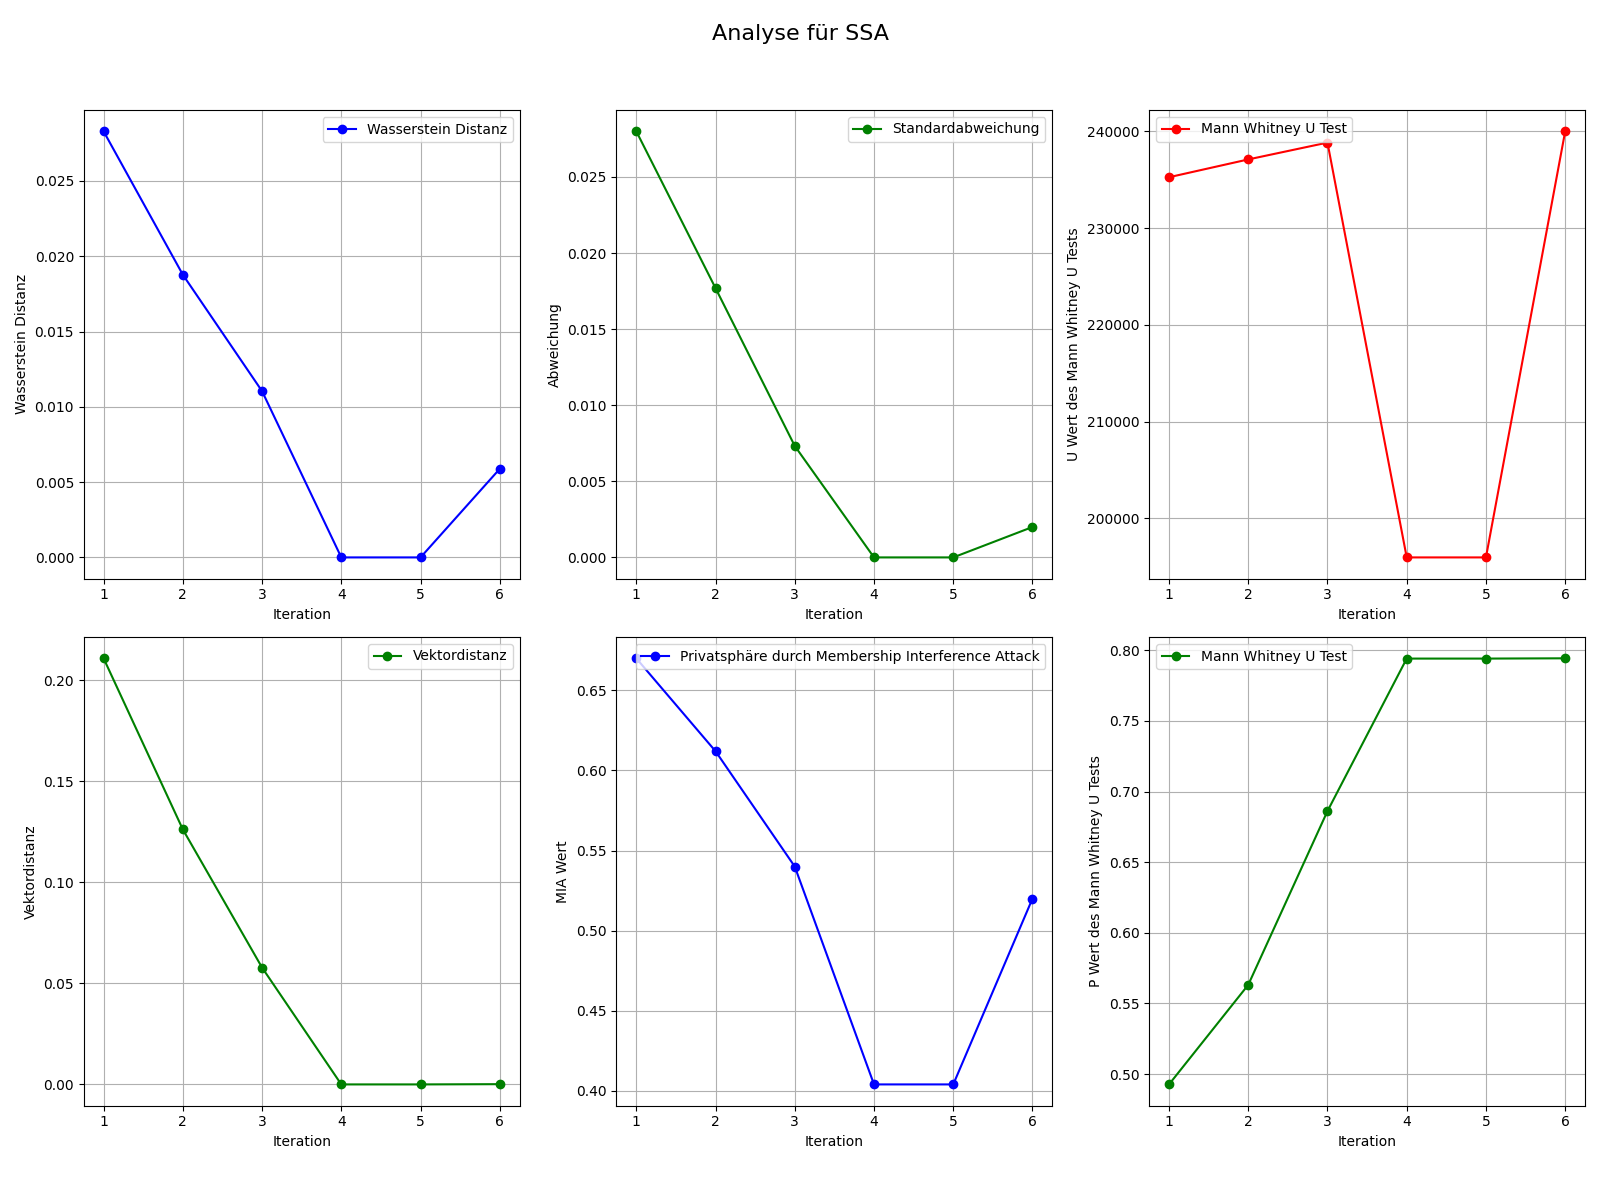
\includegraphics[width=\textwidth]{includes/figures/graphs/SSA_analysis.png}
        \caption{Analyse des SSA Algorihtmus}
        \label{fig:graphs_ssa_analysis}
    \end{minipage}
\end{figure}

\paragraph{\textbf{SSA}}
Der SSA Algorithmus zeigt, wie zu erwarten ist einen enormen Abfall in der Wasserstein Distanz sowie der Vektor Distanz und der Standardabweichung. Dies ist soweit auch verständlich, da hier mehr Informationen aus dem originalen Signal übernommen werden.
Aber der Anstieg am Ende, in der alle \ac{IMF}s genutzt werden ist interessant. Da die \ac{IMF}s aber mit steigender Position die entsprechend Elemente der Reihe aufnehmen, könnte dies im Vergleich zur gesammten analysierten Datenmenge eine Entfernung von der originalen Verteilung mitsich ziehen. Die Vektordistanz ist davon ja nicht betroffen.
Spannend ist die \ac{MIA} Metrik, da diese einen erstaunlichen hohen Wert zeigt, und dies obwohl die Vektordistanz sehr niedrig ist, also eine gute Angleichung andeutet. Schaut man auf die Ergebnisse des Mann Whitney U Tests, so steigen diese an, anstatt abzufallen. Während dies eigentlich eine Entfernung von originalen Daten darstellen sollte, zeigen die anderen Metriken genau das Gegenteil.
Dies müsste genauer untersucht werden.

\paragraph{\textbf{EMD}}
Der EMD Algorithmus zeigt ein sehr ähnliches Bild zu \ac{SSA} Algorithmus und zeigt den Abfall in  Standardabweichung, Wasserstein- und Vektor Distanz mit einem Anstieg, sofern alle \ac{IMF}s einbezogen werden.
Ein gleiches Verhalten zeigt auch die \ac{MIA} Metrik, welche einen sehr hohen Wert zeigt, obwohl die anderen Metriken eine gute Angleichung andeuten.
Hier steigt aber zwischenzeitlich der P-Wert des Mann Whitney U Tests enorm an, fällt aber wieder auf einen normalen Wert und stabilisiert sich hier. Auch dies ist interessant und sollte genauer untersucht werden.


\subsubsection{Analyse von AMIRA und Cubic Spline}
Da beide Modelle nicht auf ähnliche Weise flexibel sind wie die vorherigen Modelle und Algorithmen ist es hier nicht möglich eine Unterscheidung zwischen Iterationen oder \ac{IMF}s zu treffen.
Daher lies sich nur ein Wert jeweil berechnen.
Beide Varianten besitzen einen sehr niedrigen Wert in der Wasserstein- und Vektordistanz sowie in der Standardabweichung, relativ hohe Werte in der \ac{MIA} Metrik und einen recht hohen \textit{p} Wert im Mann Whitney U Test.



\begin{figure}[ht]
    \centering
    \begin{minipage}{0.5\textwidth}
        \centering
        \includegraphics[width=\textwidth]{includes/figures/graphs/corona_histogram_tsa.png}
        \caption{Verteilung der originalen Daten mit den synthetischen Daten des SSA Algorihtmus}
        \label{fig:graphs_ssa_histogram}
    \end{minipage}\hfill
    \begin{minipage}{0.5\textwidth}
        \centering
        \includegraphics[width=\textwidth]{includes/figures/graphs/corona_histogram_tsa_compare.png}
        \caption{Übereinstimmung des SSA Algorihtmus mit den originalen Daten}
        \label{fig:graphs_ssa_histogram_compare}
    \end{minipage}
\end{figure}




\section{Vorhersagefähigkeiten der rekusiven Modelle}
Rekusive Modell haben einen weiteren Vorteil gegenüber den generattiven Modellen. Sie sind in der Lage auch einen die nächsten Werte vorherzusagen, was bei den generativen Modellen nicht möglich ist.
Hiermit bietet sich eine weitere Möglichkeit, neue Daten zu generieren.
Forcasts sind nicht so genau und variieren stark, abhängig von der Art der Daten. Sind die Muster ihnen bekannt, können sie recht gute vorhersagen treffen, bei komplexen Daten wie beispielsweise den Corona-Fallzahlen (Siehe Abbildung \ref{fig:corona_data})
ist dies aber nicht möglich, da sich hier noch kein Muster herausgebildet hat.


\begin{figure}[ht]
    \centering
    \includegraphics[width=1\textwidth]{includes/figures/graphs/forcast.png}
    \caption{Forcast der jeweiligen rekursiven Modelle}
    \label{fig:forcast_recursive_models}
\end{figure}







\section{Zusammenfassung}
Die gesammelten Daten zeigen ein gemischtes Bild. Wird grundsätzlich ein Vergleich zwischen \ac{ML} und \ac{TSA} angestrebt, so gewinnt immer der TSA Algorithmus, sollte es ein wunsch nach Performance und Resourcenverbrauch geben.
Hier können \ac{ML} Algorithmen einfach nicht mithalten.
Schaut man auf die \ac{MIA} Werte, so ist auch hier \ac{TSA} ein wenig dem \ac{ML} Modellen vorraus. Aber dies nur sofern viele Informationen verloren gehen.
GANs und CGANs sind sehr gut im erzeugen synthetischer Daten, neigen aber zu Überanpassungen, welches sie unvorhersehbar macht. Hier lässt aber eine direkte Korrelation zwischen der Komplexität der Daten und den entstehenden Resultaten herausfinden, wie in 
Tabelle \ref{tab:autocorrelation_coefficients} zu sehen ist. Die Sinus Daten trainieren deutlich schneller als die Wetterdaten und erreichen schneller bessere Werte, wie auch an den extern beigefügten Tabellen zu erkennen ist. Aber um eine definitive Aussage zu treffen, müsste man mehrere Datensätze ähnlicher Autokorrelationswerte testen.
Dies macht die gezielte Nutzung dieser Modelle nicht einfach. Um hier ein gewünschtes Ergebnis zu bekommen, muss im Notfall experimentiert werden.


\begin{figure}[ht]
    \centering
    \begin{minipage}{0.499\textwidth}
        \centering
        \includegraphics[width=\textwidth]{includes/figures/graphs/Iteration_attacker.similaritycorona.png}
        \caption{Vektordistanz zwischen den Lösungen und dem synthetischen Daten, Trainingsdaten: corona.csv}
        \label{fig:vect_dist_corona}
    \end{minipage}\hfill
    \begin{minipage}{0.499\textwidth}
        \centering
        \includegraphics[width=\textwidth]{includes/figures/graphs/Iteration_attacker.similaritysinus.png}
        \caption{Vektordistanz zwischen den Lösungen und dem synthetischen Daten, Trainingsdaten: sinus.csv}
        \label{fig:vect_dist_sinus}
    \end{minipage}
\end{figure}

Dennoch zeigt das \ac{CGAN} eine durschnittlich deutlich bessere Performance als das normale GAN Modell.
Dies lässt sich auch an den Clustering Ergebnissen sehen. Diese sind separate im Anhang als 3D html Plots hinterlegt.
Vergleicht man die generativen Modelle mit den rekursiven Modellen, so muss eindeutig gesagt werden, dass diese eine deutlich besser Annäherung an die originalen Daten zeigen. Sie sind dabei auch deutlich schneller, benötigen also weniger Resourcen und sind einfacher zu trainieren.
Leider kommt durch die Annäherung auch eine geringe Privatsphäre, da die \ac{MIA} Metrik einen sehr niedrigen Wert zeigt.
Dann kommt dazu die uneindeutigkeit der Ergebnisse. Steigt die Komplexität, so steigt die Trainignszeit der Daten. Zu langes training kann aber zu Overfitting führen, eine zu kurze Trainingszeit zu einer schlechten Annäherung. Dies gibt dem Nutzer viel Kontrolle, aber dies nur durch ausgedehntes Testing oder einen guten loss Wert.
Hier wäre Erfahrung mit den Modellen aber wichtig.

Vergleicht man diese Werte mit den \ac{TSA} Algorithmen, so wirken diese primär erstmal deutlich attraktiver. Sie sind schneller, brauchen weniger Resourcen und sind auch recht flexibel. Selbst komplexe Zeitreihen können schnell approximiert werden.
Probleme wie Overfitting gibt es nicht. Underfitting lässt sich, jedenfalls beim Vorhandensein von genügend \ac{IMF}s, auch vermeiden, sogar steuern.
In Kombination mit dem Möglichkeiten des Frontends, welches, wie in Abbildung \ref{fig:tsa_trained_configuration} aus Sektion \ref{sec:reactTSA} hier direkt Veränderungen an der Konfiguration zulässt, ist dies ein sehr mächtiges Werkzeug, welches deutlich mehr Kontrolle an den Nutzer abgibt und ihn deutlich schneller zum Ziel führt.
Auch sind Modelle wie Amira, Cubic Spline oder das nicht implementierte Prophet in der Lage größere Datenmengen in kürzester Zeit zu verarbeiten.

Hier ist also eine Abwegung notwendig. Braucht man schnell die Daten, so sollte man auf jeden Fall zu Algorithem aus der Zeitreihenanalyse greifen. Hier erhält man direkt ein Ergebnis und kann dieses bei bedarf anpassen.
Machninelles Lernen wird bei Datenmengen interessant, welche groß und komplex sind, und bei denen meinen einen ungefähren Verlauf benötigt. 
Für komplexer Systeme, welche beispielsweise mit Außreißern klar kommen müssen, sind generative Modelle interessanter als TSA Algorithmen.


% !TeX program = xelatex

\chapter{Nutzerstudie}
\label{cha:Usability_study}

\section{Inhalte der Studie}
\label{sec:study_content}
Um eine Aussage über die Nutzbarkeit der Anwendung zu treffen, wurden zwei Verschiedene Studien durchgeführt.
Die erste Studie nutzt eine Thinking Aloud Technik, bei der die Probanden unter einer vorgegebenen Aufgabenstellung die Anwendung verwenden und dabei ihre Gedanken laut äußern.
Es wird dabei nicht nur die Aufgabe bewertet, sondern auch die wie die Nutzer Anwendung selbst warnehmen, welche Probleme sie haben und wie sie diese lösen und ob sie die Anwendung intuitiv bedienen können.
Dadurch kann im Nachhinein eine Aussage getroffen werden inwieweit die erstellten Konzepte vom Nutzer angenommen werden und ob sie so intuitiv bedienbar sind, wie angenommen.
Gerade im Bezug auf Shneidermans Golden Rules \cite{10.5555/3033040} lässt sich dies bewerten.

Die zweite Studie ist etwas größer angelegt und soll die Anwendung in einem größeren Rahmen bewerten. Hierzu wurden die Nutzer in zwei Gruppen aufgeteilt und bekommen jeweils eine leicht abgewandelte Aufgabe gestellt.
Diese können sie alleine lösen um anschliesend ihre Erfahrungen und Meinungen in einem Fragebogen zu äußern.
Der Fragebogen ist in drei Teile aufgeteilt. Im ersten Abschnitt werden die Nutzer gebeten, die Anwendung zu bewerten und ihre Erfahrungen zu äußern. Dies wird mit Hilfe des System Usability Scale (SUS) Fragebogens \cite{brooke1996sus} durchgeführt. 
Im zweiten Teil wird die mentale Leistung der Nutzer gemessen und dafür der Nasa Task Load Index (NASA-TLX) \cite{HART1988139} verwendet.
Um die in den ersten beiden Teilen in einen Kontext zu setzen, werden im dritten Teil noch einige Fragen zur Person und dem Umgang mit der Anwendung gestellt.

Der NASA-TLX Frageboge existiert seit 1988, ist anerkannt und weit verbreitet. Ziel des Fragebogens ist es zu messen, wie mental Fordernd die Anwendung ist. 
Mithilfe von 6 Fragen wird die mentale Belastung in den 6 folgenden Kategorien bewertet:
\begin{description}
    \item[Geistige Anforderung] Wie geistig anspruchsvoll war die Aufgabe?
    \item[Körperliche Anforderung] Wie körperlich anspruchsvoll war die Aufgabe?
    \item[Zeitliche Anforderung] Wie gehetzt oder eilig war das Tempo der Aufgabe?
    \item[Leistung] Wie erfolgreich waren Sie bei der Erledigung dessen, was von Ihnen verlangt wurde?
    \item[Anstrengung] Wie hart mussten Sie arbeiten, um Ihre Leistung zu erreichen?
    \item[Frustration] Wie unsicher, entmutigt, gereizt, gestresst und genervt waren Sie?
\end{description}

Die Bewertung erfolgt auf einer Skala von 1 bis 10, wobei 0 für sehr geringe Anforderung steht und 10 für sehr hohe Anforderung. Aufsummiert ergibt der finale Wert die mentale Anforderung. Ist der Wert hoch, dann muss der Nutzer sich stark auf die Anwendung konzentrieren. 
Bei einem geringen Wert hat der Nutzer wenig Probleme mit der Anwendung klar zu kommen.

Der System Usability Scale Fragebogen ist ebenfalls sehr weit verbreitet und wird seit 1986 verwendet. Er besteht aus 10 Fragen (Siehe \ref{itm:sus_questions}), die in einer 5-Punkte Likert-Skala bewertet werden. Eine 5 steht dabei für "Stimme voll zu" und eine 1 für "Stimme überhaupt nicht zu". Die Fragen sind im wechsel 
positiv und negativ formuliert, um eine Verzerrung der Ergebnisse zu verhindern. Dies macht die Auswertung ein wenig komplizierter, da die negativ formulierten Fragen umgerechnet werden müssen. Nach einer Normalisierung werden die negativen Werte umgerechnet und danach aufsummiert und mit 2.5 multipliziert.

Die Fragen sind:

\begin{itemize}
\label{itm:sus_questions}
    \item Ich denke, ich würde die Website/die App regelmäßig nutzen.
    \item Die Website/die App scheint mir unnötig kompliziert zu sein.
    \item Ich finde, die Website/die App ist einfach zu bedienen.
    \item Ich denke, ich würde technische Unterstützung benötigen, um die Website/die App nutzen zu können.
    \item Ich denke, dass die verschiedenen Funktionen der Website/des Apps gut integriert sind.
    \item Die Website/die App scheint mir zu inkonsistent.
    \item Ich glaube, dass die meisten Menschen schnell lernen können, wie man die Website/die App benutzt.
    \item Die Website/die App scheint sehr umständlich in der Nutzung zu sein.
    \item Ich fühle mich sehr sicher bei der Nutzung der Website/des Apps
    \item Ich musste viel lernen, um mich mit der Website/dem App zurechtzufinden.
\end{itemize}


\section{Studienablauf}
\label{sec:study_process}
Die für dieses Projekt gewählten Personas sind divers. Sie haben einen gewissen technischen Hintergrund, sind aber keine Experten. 
Dies erlaubt daher auch eine breite Auswahl an Teilnehmern in die Studie einzubeziehen.
Für die Studie wurden 11 Probanden ausgewählt. Die Auswahl erfolgte über persönliche Kontakte, weitere Nutzer haben die Software ausgetested, aber nicht an der Studie teilgenommen.

Schaut man sich die Hintergründe der Probanden an, so fällt auf, dass diese sehr unterschiedlich sind. Die Probanden sind zwischen 24 und 40 Jahre alt, sind in unterschiedlichen, auch nicht technischen Berufen tätig und zeigen eine ziemlich unterschiedliche technische Grundfähigkeit auf.
Es gibt bereits Teilnehmer mit einem geringen Vorwissen im Bereich der Simulationssoftware.

Da es, wie in der im Anhang beigefügten Aufgabenstellung zwei unterschiedliche Aufgaben gibt, wurden die Probanden in zwei Gruppen aufgeteilt, welche aus jeweils 5 Teilnehmern bestanden.
Teilnehmer Nr. 11 hatte beide Aufgaben durchgeführt. 
Mit außnahme einiger weniger Probanden, welche zusätzlich noch eine kurzen Thinking Aloud Technik unterzogen wurden, durften die meisten Probanen sich selber ohne weitere Unterstützung an der Aufgabe versuchen.
Da die Webanwendung auf einem Server läuft, mussten die Probanden nicht extra eine Anwendung installieren, sondern konnten diese direkt über den Browser aufrufen. Aufgabenstellung und Testdaten wurden den Probanden in einer Datei zur Verfügung gestellt.

Teilnehmer der Thinking Aloud Studie bekamen die gleiche Aufgabe gestellt, diese sollten sie aber unter überwachung durchführen und wurden gebeten, ihre Gedanken während der Aufgabenlösung laut auszusprechen. Diese, sowie ihre Interaktionen, wurden alle protokolliert.
Wichtig ist, dass die Probanden dabei nicht beeinflusst wurden und somit die Aufgabe frei und selbstständig lösen mussten.
Die Protokolle erlauben einen Einblick in die Gedanken der Nutzer und erlauben Rückschlüsse darüber, inwieweit der Nutzer die Prozesse und Möglichkeiten der Anwendung realisiert und versteht.



\section{Auswertung der Studie}
\subsection{Ergebnisse der Thinking Aloud Studie}
Die Studie wurde mit fünf Probanden durchgeführt, die aufgefordert wurden, die Aufgaben zu lösen und dabei ihre Gedanken laut auszusprechen, wie bereits in Sektion \ref*{sec:study_content} beschrieben.

Zu Beginn erhielten die Teilnehmer etwas Zeit, um sich mit der Software vertraut zu machen, da sie zuvor noch keine Erfahrungen mit dieser hatten. Dieser Schritt war entscheidend, um ihnen ein grundlegendes 
Verständnis für die Funktionsweise der Software zu vermitteln.

Während der Aufgabenbearbeitung hatten die Teilnehmer im Allgemeinen wenig Schwierigkeiten. Die meisten verstanden die Aufgabenstellung schnell und konnten durch das Durchsuchen der Menüs die benötigten Funktionen finden. 
Oft wichen sie anfangs von der eigentlichen Aufgabe ab und erforschten eigenständig die Möglichkeiten der Software. Positiv hervorgehoben wurden dabei die integrierten Tooltips.

Bei der Definition der Generierung synthetischer Daten kamen die meisten Teilnehmer gut mit dem Dialog zurecht. Der dritte Schritt, die Definition der Datenvorverarbeitung, stellte sich jedoch als verwirrend heraus. 
Die Teilnehmer waren sich über die Bedeutung der einzelnen Optionen und deren Auswirkungen auf die Daten unsicher. Hinzu kam, dass das verwendete Schema zwar eine Beschreibung für alle Optionen bot, die eingesetzte rsjf-Bibliothek jedoch 
keine Erklärungen für die Auswahl der Imputationsalgorithmen bei den Radio Buttons zur Verfügung stellte. Drei der Nutzer entdeckten zudem nicht die Möglichkeit, sich einen Graphen der Daten anzeigen zu lassen, obwohl dieser 
direkt unter der Konfiguration zu finden war. Der Teilnehmer, der den Graphen entdeckte, war sich jedoch nicht bewusst, dass man einzelne Graphen dynamisch ausblenden kann, und konnte daher nur wenig Nutzen aus der Visualisierung ziehen.

Nach dem Absenden der Konfiguration hatten die Teilnehmer wenig Schwierigkeiten, entweder testweise die Graphen zu verschieben und zu speichern oder das Training der Modelle zu starten. Besonders positiv wurde die 
prozentuale Statusanzeige während des Trainings der Modelle aufgenommen. Bei der Erstellung der Projekte hatte ein Teilnehmer bereits an der Nutzerstudie der ursprünglichen Anwendung teilgenommen und verfügte daher über 
einen guten Überblick über die notwendigen Schritte. Die anderen Teilnehmer hatten jedoch Schwierigkeiten, die Unterscheidung zwischen Projekten, Tracks und Datasets zu verstehen. Da diese Struktur jedoch zweckmäßig ist 
und einen bestimmten Nutzen verfolgt, könnten zukünftige Einarbeitungen diese Probleme beheben.

Auffällig war, dass viele Teilnehmer den Informationsbutton nicht näher betrachteten. Dieser bietet eine Visualisierung der Websockets, also der trainierenden Modelle und der gesendeten Projekte. Die Personen, die ihn 
benutzten, waren verwirrt, als sie keine Aktivität sahen, weil gerade nichts trainiert wurde. Hier ist also weitere Arbeit nötig, um die Nutzer besser über die Bedeutung und Funktion dieser Anzeige zu informieren.

\subsection{Auswertung der Fragebögen}
\label{sec:results_of_user_experience}
Die Fragebögen wurden von allen Teilnehmern ausgefüllt, einschließlich jener, die an der Thinking Aloud Technik teilnahmen. Die einzelnen Ergebnisse sind in der Tabelle \ref{tab:probanden} im Anhang dargestellt. 
Generell lässt sich sagen, dass die Nutzer die Anwendung als gut bedienbar empfanden. Die durchschnittlichen Ergebnisse auf der SUS-Skala lagen bei 76.32, was darauf hindeutet, dass die Anwendung als 
benutzerfreundlich wahrgenommen wurde. Mental fühlten sich die Nutzer nicht stark gefordert, was sich in einem durchschnittlichen TLX-Wert von 36.5 widerspiegelt, ein Indikator dafür, dass die Aufgaben ohne große Anstrengungen gelöst werden konnten.

Besonders interessant ist der Vergleich der Ergebnisse der Fragebögen im Zusammenhang mit Alter und technischer Begabung der Teilnehmer (siehe Abbildung \ref{fig:3dplot_tlx_sus}). Hierbei zeigte sich, 
dass Teilnehmer mit geringerer technischer Begabung die Anwendung weniger fordernd fanden, während jene mit durchschnittlicher Begabung dies als anspruchsvoller empfanden. Teilnehmer mit hoher technischer 
Begabung fanden die Aufgaben wiederum leichter. Dies mag zunächst kontraintuitiv erscheinen, aber unter Berücksichtigung der Beobachtungen aus der Thinking Aloud Studie ergibt sich ein schlüssiges Bild: Nutzer mit geringer technischer Begabung gingen erstaunlich schnell durch die Anwendung und klickten die meisten Funktionen direkt an, ohne sich zunächst auf die Aufgabe zu konzentrieren. Bei Nutzern mit durchschnittlichem technischen Verständnis war dies nicht der Fall; sie verhielten sich deutlich zögerlicher.

\begin{figure}[h]
    \centering
    \includegraphics[width=\textwidth]{includes/figures/study/3dplot.png}
    \caption{Grafische Darstellung der Ergebnisse des NASA-TLX und SUS-Fragebogens in Abhängigkeit des Alters und der technischen Begabung}
\label{fig:3dplot_tlx_sus}
\end{figure}

Eine Korrelation des Alters mit dem Testergebnis war nicht erkennbar. Die Altersverteilung war jedoch zu klein, um aussagekräftige Schlussfolgerungen zu ziehen, insbesondere im Hinblick auf die technische 
Begabung. Während sich die technische Begabung bei den Teilnehmern in den mittleren Zwanzigern noch recht gut verteilte, war sie bei den älteren Teilnehmern deutlich höher.

Wie in Abbildung \ref{fig:study_sus} dargestellt, war insbesondere bei Frage 1, \textit{'Ich denke, ich würde die Website/die App regelmäßig nutzen.'}, eine hohe Zustimmung zu verzeichnen. Die Nutzer wurden 
gebeten, sich in die Situation zu versetzen, solch eine Software zu benötigen. Obwohl die meisten Teilnehmer in einer solchen Situation nicht sind, war es notwendig um über den Fragebogen eine valide Aussage zu erhalten.

\begin{figure}[ht]
    \centering
    \begin{minipage}{0.5\textwidth}
        \centering
        \includegraphics[width=\textwidth]{includes/figures/study/tlx.png}
        \caption{Auswertung des NASA-TLX Fragebogens}
        \label{fig:study_tlx}
    \end{minipage}\hfill
    \begin{minipage}{0.5\textwidth}
        \centering
        \includegraphics[width=\textwidth]{includes/figures/study/sus.png}
        \caption{Auswertung des SUS Fragebogens}
        \label{fig:study_sus}
    \end{minipage}
\end{figure}


% !TeX program = xelatex

\chapter{Ausblick}
\label{ch:ausblick}

\section{Einführung neuer Modelle}
In dieser Arbeit lag der Fokus auf rekursiven und generativen Modellen. Variational Autoencoder, die aktuell große Beliebtheit genießen, stellen eine vielversprechende Erweiterung dar. Diese Autoencoder sind besonders effektiv in der 
Generierung synthetischer Daten, da sie fähig sind, aus erlernten Datenmustern realistische und vielfältige Beispiele zu erzeugen. Für Variational Autoencoder wurde in der Testumgebung bereits ein Grundgerüst entwickelt, 
jedoch konnte aufgrund zeitlicher Beschränkungen keine umfassende Bearbeitung zur Erzielung aussagekräftiger Ergebnisse vorgenommen werden. Eine Weiterentwicklung in diesem Bereich könnte daher sehr fruchtbar sein.



\section{Erweiterungsmöglichkeiten innerhalb des \ac{ML} Bereiches}
In der Auswertung wurde viel über die tsgm Modelle geschrieben. Sie produzierten gute Ergebnisse, nur kamen sie mit Hardwareanforderungen und einer nicht direkt lösbaren Speicherinffizienz.
Dies macht sie ungeeignet für den Einsatz in der geschriebenen Django API. Wenn sich dieser Umstand ändert, wäre es möglich die tsgm Modelle in die API zu integrieren.
Hierzu müssten lediglich die Datenbankeinträge dafür erstellt werden. Im Testprojekt sind diese bereits an das in der API genutzte Konzept angepasst worden.
Da die Modelle auch zeitlich nicht mit den doch relativ kurzen Trainingszeiten der nativen Modelle mithalten können, aber bereits mit weniger Iterationen nutzbare Ergebnisse liefern, wäre hierfür auch noch ein Informationskonzept zu erstellen.
Der letzte Punkt betrifft wie Erstellung von Projects. Die tsgm Modelle können zwar ebenso aus der Datenbank geladen werden, bemätogen aber einen anderen Ladeprozess.
Dieser ist weitestgehend integriert, aber kann zeitaufwendig sein. Da lange Prozesse nicht in das REST Prinzip passen, bräuchte es hier eine Websocketschnittstelle, 
die den Ladeprozess überwacht und die fertig generierten Daten an die Spring API sendet. Da diese aber über das Frontend angesprochen wird, muss dieses auch die Websockets integrieren und ist daher auch zu ändern, wodurch eine grundsätzlich kleine Änderung 
der Funktionalitäten eine große Änderung der Gesammtarchitektur nach sich zieht.

Darüber hinaus kann auch mit freieren Parametern experimentiert werden. So kann die Anzahl der Neuronen in den Layern verändert werden, oder die Anzahl der Layer selbst.
Dies bedeutet aber einen enormen Validierungsaufwand, da nicht alle Kobminationen sinnvoll sind oder gar funktionieren. Eine weitere Möglichkeit ist die stärkere Integration von Loss-Funktionen. Diese wird aktuell nur sporadisch genutzt.

Aufgrund von erhobenen Statistiken könnten auch vorschläge erstellt werden. Über ein dynamisches Auswahlverfahren könnten dem Nutzer passende Modelle mit passenden Konfigurationen vorgeschlagen werden, oder das dieser sich um die genauen Parameter zu kümmern hat.
Hierfür kann ein \acf{LLM} genutzt werden, welches in einem Dialog mit dem Nutzer die Parameter erfragt und direkt mit der API kommuniziert. Dies würde die Nutzerfreundlichkeit enorm erhöhen.
Die Grundlagen hierfür sind bereits teilweise gelegt, da es eine umfangreiche OpenAPI Definition gibt, mti welcher LLMs umgehen können.

\section{Erweiterungsmöglichkeiten außerhalb des TSA Bereiches}
Gerade die rekursiven Modelle sind in der Lage eine Forcast zu erstellen. Eine durchaus interessante und praktische Funktion.
Da dies grundsätzlich auch durch \ac{IMF}s möglich ist, wäre eine mögliche Erweiterung hier auch interessant.
Während die Grundlagen hierfür in der Testumgebung bereits geschaffen wurden, waren die Ergebnisse noch nicht zufriedenstellend und wurden daher nicht in die Auswertung mit übernommen.
Dennoch bietet sich hier ein Potzenzial, welches es zu nutzen gilt. Ansätze wie Fouriertransformationen könnten hierbei helfen.
Modelle wie Prophet könnten weitere interessante Ansätze liefern, welche es zu untersuchen gilt.

\section{Erweiterungsmöglichkeiten innerhalb des Frontends}
Obwohl die Studie eine insgesamt gute User Experience des Frontends bestätigt, gibt es Bereiche, die verbessert, vereinfacht oder fehlertoleranter gestaltet werden könnten. 
Der umfangreiche Einsatz von Json Schema bietet zwar flexible Erweiterungsmöglichkeiten für die Funktionalitäten, zeigt jedoch im Bereich der Benutzerunterstützung und Hilfestellungen Grenzen auf.

\section{Testabdeckung}
Eine Erhöhung der Testabdeckung wäre ein wichtiger Schritt zur weiteren Verbesserung der Anwendung. Dazu ist die Integration von Testcontainern notwendig, sowie die Einbindung einer 
gemeinsamen Datenbankinstanz in die Testumgebung, um effektive Unit Tests zu ermöglichen.

Für Component- und Systemtests, die auch das Frontend einbeziehen, wären Tools wie Pact und Playwright geeignet. Pact ermöglicht das Testen der Kommunikation zwischen zwei Systemen, 
indem ein simulierter Pactserver die Anfragen des zu testenden Systems empfängt und entsprechende Antworten liefert. Dieser Prozess kann automatisiert werden. Playwright ist für das Testen des Frontends vorgesehen, wobei ein Browser gestartet wird, der bestimmte Aktionen ausführt und die Ergebnisse überprüft. Diese Tests können direkt in Java integriert und automatisiert ausgeführt werden.

Eine unzureichende Testabdeckung oder das Fehlschlagen von Tests könnte dazu führen, dass die Pipeline automatisch abgebrochen wird, um die Qualität der Anwendung zu gewährleisten.
% !TeX program = xelatex

\chapter{Fazit}
\label{cha:conclusion}

\section{Ergebnisse der Nutzererfahrung}
\label{sec:results_of_user_experience}
Die Nutzererfahrung war der zweite wichtige Punkt innerhalb der Arbeit.
Nutzer müssen ihre Aufgaben möglichst schnell und einfach erledigen können.
Aus der Studie ließ sich ableiten, dass die Nutzer die Aufgaben recht problemlos erledigen konnten, sobald sie verstanden hatten, was zu tun ist.
An diesen Punkt zu gelangen, war jedoch nicht immer einfach. Dies ist zwar nicht verwunderlich, da die Nutzer die Aufgaben zum ersten Mal sahen, aber dennoch ein wichtiger Punkt.

Die Ergebnisse der Evaluation zeigen, dass die Zeitreihenzerlegung in den meisten Fällen bessere Ergebnisse liefert. Dies ist vor allem darauf zurückzuführen, 
dass die Zeitreihenzerlegung die Datenpunkte der Originaldaten nicht verändert, sondern nur deren Anzahl reduziert. Die generativen Modelle hingegen erzeugen neue Datenpunkte, die nicht 
immer den Originaldaten entsprechen. Dies führt zu einer höheren Abweichung der generierten Daten von den Originaldaten.

\section{Auswertung der umgesetzten Anforderungen}
Zu Beginn der Arbeit wurde eine Liste an Anforderungen (siehe \ref{list:requirements}) aufgestellt, welche im Verlauf der Arbeit erfüllt werden sollten. 
Diese Anforderungen werden nun einzeln ausgewertet.

\paragraph*{Vielseitige Datenintegration und Unterstützung mehrerer Datenformate}
Die Software unterstützt Datenformate wie CSV, JSON und NumPy-Arrays, welche einen großen Teil der gängigen Datenformate für Zeitreihen abdecken sollten.
Die Daten können über die Weboberfläche oder über die \ac{REST} \ac{API} importiert werden, beispielsweise über Tools wie curl oder Postman\footnote{Postman ist eine API-Plattform, \url{https://www.postman.com/}}.

\paragraph*{Effiziente Datenübertragung, -validierung und Systemressourcennutzung}
Die Datenübertragung, insbesondere im Frontend, ist zweiteilig aufgebaut. Grundsätzlich können die Daten in einem separaten Bereich hochgeladen und durch die Django-API überprüft werden. 
Die zweite Möglichkeit, Daten hochzuladen, besteht bei der Erstellung von Konfigurationen. Um die Datenübertragung hier möglichst gering zu halten, werden die Daten erst hochgeladen, wenn die Konfiguration vollständig ist. Der Preview ist hiervon ausgenommen.
Um die Anzahl an Datenbankoperationen möglichst gering zu halten und damit die Ressourcenauslastung niedrig, werden hier Daten nur gecacht und nicht persistiert, sofern keine bereits persistenten Daten vorhanden sind.
Das Konzept der Datenvalidierung wurde in Sektion \ref{sec:djangoDataPreprocessing} genauer erläutert.

\paragraph*{Benutzerorientierte Datenauswahl und -vorverarbeitung sowie Verwaltung:}
Um die Datenauswahl für Nutzer flexibel zu gestalten, wurde ein zweischneidiges Konzept implementiert. 
Da gerade bei Zeitreihen die Datenmenge schnell sehr groß werden kann, werden nur die einzelnen Zeitreihen an die Konfiguration angehängt, um ungewollte Daten in einer Konfiguration zu vermeiden.
Um dennoch die Datenauswahl effektiv zu gestalten, sind alle Zeitreihen an ein Dokument gebunden, welches referenziert werden kann und alle Zeitreihen enthält. Dies kann auch in der passenden Übersicht den gewünschten Anforderungen angepasst werden.

Die Vorverarbeitungsschritte werden dem Nutzer über anpassbare und erweiterbare JsonSchemas zur Verfügung gestellt. Diese sind in der Django-API einfach erweiterbar.
Es existieren Imputations- sowie Transformationsalgorithmen, welche die Daten vorverarbeiten können. Der Nutzer hat hier freie Auswahlmöglichkeiten und kann die Transformationsalgorithmen seinen speziellen Anforderungen anpassen.

\paragraph*{Visuelles Feedback, Datenexploration und transparente Ergebnisdarstellung}
Für visuelle Rückmeldungen wurde viel mit Graphen und Diagrammen innerhalb der Weboberfläche gearbeitet. Diese sind teilweise interaktiv und erlauben somit einen tiefen Einblick in die Unterschiede, 
die beispielsweise durch die Datenverarbeitung entstehen.
Für die Fehlerbehandlung wurde eine eigene Komponente dem Frontend hinzugefügt. Die Fehlermeldungen aus den APIs sind standardisiert und auch mit i18n-Keys versehen, wodurch die spezifischen Fehler direkt in der Nutzersprache angezeigt werden können.
Durch die Implementierung von Websockets ist eine direkte Status-/Fortschrittsanzeige möglich, welche den Nutzer über den aktuellen Stand der Verarbeitung informiert.


\paragraph*{Sicherheit, Privatsphäre und sicherer Umgang mit Benutzerdaten}
Die Sicherheit der Anwendung ist mehrschichtig aufgebaut. Ein zentraler Punkt sind die APIs, die sowohl durch JWT-Authentifizierung als auch durch \ac{CSRF}- und \ac{CORS}-Richtlinien geschützt sind. 
Invalide Tokens haben nur Zugriff auf wenige öffentliche Endpunkte.
Die Weboberfläche ist durch Routenschutz abgesichert und lässt nicht eingeloggte Nutzer lediglich auf die Login-Seite. Aktuell ist die Anwendung nur über HTTP erreichbar, jedoch kann Traefik 
problemlos konfiguriert und mit entsprechenden Zertifikaten ausgestattet werden.

Die spezifischen Daten der Nutzer werden in der Datenbank gespeichert, allerdings wurde auf eine zusätzliche Verschlüsselung der einzelnen Datenbankspalten verzichtet. Der Zugriff auf die 
entsprechenden Daten ist über die API nur für berechtigte Nutzer möglich, während die Datenbank selbst durch Docker Compose abgesichert ist und keinen Port nach außen freigibt, also nur innerhalb des Docker-Netzwerks erreichbar ist. Dies sollte ein ausreichendes Sicherheitsniveau für die Nutzerdaten bieten.

\paragraph*{Trainieren der Modelle und Bereitstellung einer Vielzahl von Algorithmen}
Im Frontend werden aktuell vier verschiedene \ac{ML}-Algorithmen zur Datengenerierung angeboten, von denen zwei rekursiv und die anderen beiden generativ sind. Für die Tests wurden fünf 
weitere Modelle geprüft: zwei rekursive und drei generative. Die rekursiven Modelle könnten direkt in die Anwendung integriert werden, während die generativen Modelle aufgrund unzureichender Performance bezüglich der genutzten Hardware nicht Bestandteil der Anwendung sind.

Im Bereich der \ac{TSA} werden \ac{EMD}, \ac{SSA}, Amira und Cubic Spline angeboten. Der Algorithmus Prophet, der in der Testumgebung vorhanden ist, kann jedoch keine synthetischen 
Daten erzeugen und wurde daher nicht in die Anwendung integriert.


\paragraph*{Benutzerschnittstelle, Benutzererfahrung und intuitive Konfiguration der Algorithmen}
Die Auswertung der SUS- und TLX-Studie (siehe \ref{sec:results_of_user_experience}) zeigt positive Ergebnisse. Der SUS-Score von 76.32 wird als \textit{gut} eingestuft und der 
TLX-Score von 36.5 deutet auf eine \textit{geringe mentale Belastung} hin, was insgesamt eine gute Benutzererfahrung widerspiegelt. Die intuitive Konfiguration der Algorithmen wurde durch 
den Einsatz von JsonSchema erreicht. Allerdings könnte, laut der Thinking Aloud Studie, noch Raum für Verbesserungen bestehen.

\paragraph*{Dokumentation, Fehlerbehandlung, Überwachung und Deployment}
In der Implementierungsphase wurde die Dokumentation nicht vollständig abgeschlossen. Für die umfassende Dokumentation, die verschiedene Bereiche umspannt, wurde sich für eine Hugo-Dokumentation 
entschieden. Hugo, ein Static Site Generator, wie in Paragraph \ref{par:hugo} erwähnt, ermöglicht es, komplexe Abhängigkeiten mit Mermaid\footnote{Mermaid ist eine Diagrammsprache, https://mermaid-js.github.io/mermaid/} 
zu visualisieren. Die Dokumentation liegt in Markdown-Dateien vor und wird bei jedem Deployment aktualisiert und integriert. Die OpenAPI Spezifikation wurde für die Dokumentation der 
API-Schnittstellen genutzt, zugänglich im lokalen Deployment. Die Swagger.yaml-Dateien werden im externen Anhang bereitgestellt, ebenso wie eine Postman-Konfiguration.

Der Fehlerbehandlungsprozess könnte noch verbessert werden, da nicht alle Fehlercodes übersetzt sind und einige technische Fehlerbeschreibungen für Nutzer unklar sein könnten. Insbesondere 
die Websocket-Komponenten benötigen eine bessere Fehlerbehandlung.

Das Projekt wird durch Prometheus und Graylog überwacht. Graylog muss initial konfiguriert werden und kommuniziert über das UDP-Protokoll. Sobald eingerichtet, werden Logs angezeigt und können 
gefiltert werden. Prometheus ist bereits konfiguriert und zeigt die relevanten Metriken an. Die Konfigurationen werden im externen Anhang bereitgestellt und sind Teil des Deployment-Projekts.

Das automatische Deployment erfolgt über einen GitLab Runner und eine entsprechende GitLab-CI-Konfiguration, wobei Docker Images erstellt und auf einem lokalen Server bereitgestellt werden.



\section{Ergebnisse der Evaluation}
Aufbauend auf den Ergebnissen aus Kapitel \ref{cha:events_and_evaluation} lässt sich ein Fazit ziehen, das die Ergebnisse zusammenfasst und einen Ausblick auf mögliche weitere Forschungen gibt.
Die Ergebnisse der Evaluation können in verschiedene Punkte gegliedert werden.

\paragraph*{Effizienz}
Effizienz ist grundsätzlich ein wichtiges Thema.
Vergleicht man die beiden Ansätze, so ist die Zeitreihenzerlegung deutlich effizienter als maschinelles Lernen. Dies war jedoch von Anfang an klar. 
Innerhalb der \ac{ML}-Ansätze gibt es aber auch deutliche Unterschiede. Die nativen Keras-Modelle sind bei weitem effizienter als die aus externen Bibliotheken, nutzen jedoch auch deutlich weniger Parameter.
Wie jedoch in Sektion \ref{sec:similarity_of_time_series} dargestellt wurde, bedeutet dies keinesfalls schlechtere Ergebnisse. Benötigt man jedoch Daten, die sehr nah an den Originaldaten liegen, 
so eignen sich rekursive Modelle besonders gut, da sie sehr schnell sind und bereits mit wenigen Iterationen eine gute Nachbildung liefern können.

\paragraph*{Genauigkeit}
Die Genauigkeit der generierten Daten ist ein weiterer wichtiger Punkt.
Ziel war es, synthetische Daten zu schaffen, die das Original abbilden, um einen Mehrwert zu bieten. Ausreißer an den falschen Stellen oder grundsätzlich andere Verläufe 
können beispielsweise zu falschen Schlussfolgerungen führen.
Betrachtet man daher die Ergebnisse der beiden Methoden, so liefert die Zeitreihenzerlegung in den meisten Fällen eine deutlich bessere Annäherung. Generative Modelle fügen der neuen Zeitreihe 
Variabilität hinzu, die stark schwankt und von der Anzahl an Trainingsiterationen und der Korrelation der Originaldaten abhängt.
Rekursive Modelle hingegen liefern eine schnelle Abbildung der Daten, tendieren nicht zum Overfitting und sind in der Lage, auch Prognosen zu treffen.

\paragraph*{Limitationen}
Das Projekt war recht umfangreich. Es wurden insgesamt 4 \ac{TSA}-Algorithmen und 9 \ac{ML}-Modelle getestet, doch bieten sich hier weitere Möglichkeiten. Auch könnte ein gezieltes 
Fine-Tuning der Parameter die Ergebnisse in manchen Bereichen deutlich verbessern.
Sollten die Tests mit viel mehr Daten durchgeführt werden, könnte eventuell auch eine Korrelation zwischen der Komplexität oder Autokorrelation der Daten und ihrer Effizienz und Genauigkeit 
festgestellt werden. In den Tests wurde zwar eine festgestellt, diese kann aber aufgrund der geringen Datenmenge nicht als allgemeingültig angesehen werden.


\subsection{Schlusswort}
Abschließend lässt sich sagen, dass sowohl ML- als auch TSA-Ansätze ihre Vor- und Nachteile haben. Generative Modelle eignen sich am besten für ähnliche Daten, während rekursive Modelle und TSA-Algorithmen 
sich den Originaldaten schnell annähern, aber schneller und ressourceneffizienter sind. Diese Nachteile können durch sorgfältige Auswahl des Algorithmus und geeignete Vorverarbeitungsschritte ausgeglichen werden.


\cleardoublepage
\pagenumbering{roman}

\appendix

%todo: Add appendices

\chapter{Appendix}


\begin{longtable}{rrrrllr}
        \caption{Teilnehmerbewertungen: Der SUS-Score sowie der TLX-Score reichen bis 100. Ein hoher SUS-Score und ein niedriger TLX-Score sind erstrebenswert. Die technische Erfahrung wurde auf einer Skala von 0 (kein technisches Verständnis) bis 9 (sehr gutes technisches Verständnis) bewertet.}\label{tab:probanden} \\
        \toprule
        Alter & technische Begabung & SUS   & TLX   & Vorwissen & Beruf               & Aufgabe                                                                                                                                                                                                                                \\
        \midrule
        \endfirsthead
        \multicolumn{7}{c}%
        {\tablename\ \thetable\ -- \textit{Weitergeführt auf der nächsten Seite}}                                                                                                                                                                                                                                              \\
        \toprule
        Alter & technische Begabung & SUS   & TLX   & Vorwissen & Beruf               & Aufgabe                                                                                                                                                                                                                                \\
        \midrule
        \endhead
        \midrule
        \multicolumn{7}{r}{\textit{Weiterführung der vorherigen Seite}}                                                                                                                                                                                                                                                        \\
        \endfoot
        \bottomrule
        \endlastfoot
        25    & 5                   & 79.16 & 42.59 & 8         & Stylist             & 1                                                                                                                                                                                                                                      \\
        25    & 1                   & 87.50 & 27.77 & keine     & /                   & 2                                                                                                                                                                                                                                      \\
        31    & 5                   & 75.00 & 38.88 & keine     & Elektroniker        & 1                                                                                                                                                                                                                                      \\
        25    & 9                   & 77.08 & 33.33 & keine     & E-Learning Producer & 1                                                                                                                                                                                                                                      \\
        24    & 8                   & 85.41 & 31.48 & ja        & Studium             & 2                                                                                                                                                                                                                                      \\
        34    & 3                   & 77.08 & 44.44 & /         & /                   & 2                                                                                                                                                                                                                                      \\
        24    & 1                   & 75.00 & 27.77 & None      & Wirtschaftsstudent  & 2                                                                                                                                                                                                                                      \\
        24    & 4                   & 75.00 & 37.03 & wenig     & Sachbearbeiter      & 1                                                                                                                                                                                                                                      \\
        40    & 8                   & 89.58 & 42.59 & /         & /                   & /                                                                                                                                                                                                                                      \\
        27    & 2                   & 81.25 & 29.62 & none      & Historian           & 1                                                                                                                                                                                                                                      \\
        26    & 6                   & 37.50 & 46.29 & Simulink  & Student             & 2                                                                                                                                                                                                                                      \\
\end{longtable}





\section{Weitere Tabellen}
Alle weiteren Daten, Tabellen, Grafiken und HTML Plots sind im externen Anhang dieser Arbeit beigefügt. Diese sind zu groß oder unmöglich in dieser Arbeit darzustellen.





\includepdf[pages=-]{pdfs/Aufgabe.pdf}

% List of Abbreviations
%todo: Include your abbreviations into includes/acronyms.tex

\label{study_task_ger}
\chapter*{List of Abbreviations}
\addcontentsline{toc}{chapter}{List of Abbreviations}

% ========================================================================= CALLING
% \ac{abbr.}         % default:	full at first call, short (abbr.) else
% \acs{abbr.}        % short: 	abbr.
% \acf{abbr.}        % full: 	abbreviation (abbr.)
% \acl{abbr.}        % long: 	abbreviation
%
% for plural forms, add a -p: \acp, \acsp, \acfp, \aclp

% ========================================================================= CREATION
% \acro{POSF}{Partly Open Software Family}
% \acroplural{POSF}[POSFs]{Partly Open Software Families}

\begin{acronym}[SEPSEP]
	\acro{TSA}{Time Series Analysis}
	\acro{PCA}{Principal Component Analysis}
	\acro{LFR}{Learning Fair Representations}
	\acro{TSD}{Time Series Decomposition}
	\acro{ML}{Machine Learning}
	\acro{GAN}{Generative Adversarial Network}
	\acro{LSTM}{Long Short-Term Memory}
	\acro{UCD}{User Centered Design}
	\acro{RNN}{Recurrent Neural Network}
	\acro{ANN}{Artificial Neural Network}
	\acro{IMF}{Intrinsic Mode Function}
	\acro{HSA}{Hilbert Spectral Analyse}
	\acro{EMD}{Empirical Mode Decomposition}
	\acro{HHT}{Hilbert-Huang Transform}
	\acro{Extrema Extending Method}{EEM}
	\acro{SSA}{Singular Specturm Analysis}
	\acro{SVD}{Singular Value Decomposition}
	\acro{API}{Application Programmable Interface}
	\acro{MMD}{Maximum Mean Discrepancy}
	\acro{MUI}{Material-UI}
	\acro{SPA}{Single-Page-Applikation}
	\acro{KLD}{Kullback-Leibler Divergenz}
	\acro{t-SNE}{t-Distributed Stochastic Neighbor Embedding}
	\acro{Isomap}{Isometric Mapping}
	\acro{UMAP}{Uniform Manifold Approximation and Projection}
	\acro{GAN}{Generative Adversarial Network}
	\acro{WGAN}{Wasserstein Generative Adversarial Network}
	\acro{TGAN}{Time Series Generative Adversarial Network}
	\acro{TCGAN}{Time Series Convolutional Generative Adversarial Network}
	\acro{CGAN}{Conditional Generative Adversarial Network}
	\acro{RAM}{Random Access Memory}
	\acro{CPU}{Central Processing Unit}
	\acro{GB}{Gigabyte}
	\acro{CICD}{Continuous Integration Continuous Delivery}
	\acro{ACF}{Autokorrelationsfunktion}
	\acro{FFT}{Fast Fourier Transformation}
	\acro{MIA}{Membership Inference Attack}
	\acro{LLM}{Language Level Model}
	\acro{REST}{Representational State Transfer}
	\acro{CSRF}{Cross-Site Request Forgery}
	\acro{CORS}{Cross-Origin Resource Sharing}
	\acro{UI}{User Interface}
	\acro{ELK}{Elasticsearch Logstash Kibana}

\end{acronym}	

%%%%%%%%%%%%%%%%%%%%%%%%%%%%%%%%%%%%%%%%%%%%%%%%%%%%%%%%%%%%%%%%
% THE FOLLOWING WILL GENERATE LISTS AUTOMATICALLY
% DO NOT CHANGE THE CODE BESIDES THE LISTS' ORDER

% List of Definitions
% List of Figures
\listoffigures
% List of Tables
\listoftables
% List of Listings
\renewcommand{\lstlistlistingname}{Codeverzeichnis}
\lstlistoflistings
% List of Formulas
\renewcommand{\listtheoremname}{Liste an Formeln}g
\listoftheorems[ignoreall,show={formula}]
% Bibliography
\printbibliography %\printbibliography[heading=bibintoc] if ToC entry desired

\end{document}
